% ======================================================== 
% DEV1 - Développement I (Algorithmique et langage Java)
% HE2B - ESI
%
% Syllabus
%                                     Marco Codutti
%                                     Pierre Bettens
% ======================================================== 

\documentclass[a4paper,doubleside,11pt]{book}

%=========================
% Les styles
%=========================
% ===============================================================
%       Feuille de style LaTeX pour un syllabus à l'ESI
% ---------------------------------------------------------------
% On suppose qu'on travaille avec la classe book
%                                                   Marco Codutti
% ===============================================================


% ===================================================
%   Style commun à tout type de document
% ===================================================
% ===============================================================
%   Partie commune à tout type de document : 
%		syllabus, td, interro...
% ===============================================================

\usepackage[utf8]{inputenc}     % Source en UTF8, permet les accents
\usepackage[T1]{fontenc}        % Permet les accents dans le PDF
\usepackage[francais]{babel}    % Gestion du français
\usepackage{textcomp}	        % Plein de symboles
\usepackage{lmodern}            % Police de caractères moderne
\usepackage[
	hmargin=3.5cm,
	vmargin=3cm
	]{geometry} 				% Géométrie de la page
\usepackage{caption}
\usepackage{subcaption}


% ===================================================
%   Style des (sub)sections
% ===================================================

% Permet d'avoir les numéros de (sub)sections dans la marge
% Tiré de "Latex Howtos" de Sébastien Combéfis
% -------------------------------------------------------------
\makeatletter
\def\@seccntformat#1{\protect\makebox[0pt][r]{\csname the#1\endcsname\quad}}
\makeatother


% ===================================================
%   Style des paragraphes
% ===================================================

% Enlever l'indentation de chaque première ligne de paragraphe
% + léger espace entre les paragraphes.
% http://www.ctan.org/pkg/parskip
% -------------------------------------------------------------
\usepackage{parskip}
\raggedbottom

% Pour barrer d'une croix tout un block
% \begin{wrong}\begin{LDA}...\end{LDA}\end{wrong}
\usepackage{environ}
\NewEnviron{wrong}{%
%	\begin{tikzpicture}
%		\node (box){\begin{minipage}{\linewidth}\BODY\end{minipage}};
%		\draw[gray] (box.north west) -- (box.south east); % pour un trait en diagonale principale
%		\draw[gray] (box.south west) -- (box.north east); % pour un autre trait en diagonale 
%	\end{tikzpicture}
	\begin{minipage}{\linewidth-2mm}\BODY\end{minipage}
	\hskip-5mm
	
\includegraphics[width=1cm]{icon/dont}
	}
\NewEnviron{correct}{%
%	\begin{tikzpicture}
%		\node (box){\begin{minipage}{\linewidth}\BODY\end{minipage}};
%		\draw[gray] (box.north west) -- (box.south east); % pour un trait en diagonale principale
%		\draw[gray] (box.south west) -- (box.north east); % pour un autre trait en diagonale 
%	\end{tikzpicture}
	\begin{minipage}{\linewidth-2mm}\BODY\end{minipage}
	\hskip-5mm
	%\includegraphics[width=1cm]{icon/do}
	}
	
% ===================================================
%   Paragraphes spéciaux
% ===================================================

%---------------------------------------
% Citation en début de chapitre
%---------------------------------------
\newenvironment{Exergue}{%
	\begin{quote}
	\itshape
	}{
	\end{quote}
	\vskip2\baselineskip
	}

%---------------------------------------
% \begin{Emphase}...\end{Emphase}
% Met en évidence un ou des paragraphes
% début de cadre en gris
%---------------------------------------
\newenvironment{Emphase}%
  {%
	\par\nobreak%
	\bgroup%
		\color{gray}%
		\hskip-0.3cm%
		\rule{4cm}{0.5pt}%
		\hskip-4cm%
		\rule[-2em]{0.5pt}{2em}%
		\vskip-2.5em%
	\egroup%
  }{%
	\par\nobreak%
	\bgroup%
		\color{gray}%
		\vskip-2em%
		\hskip-0.3cm%
		\rule{0.5pt}{2em}%
		\rule{4cm}{0.5pt}%
		\hskip-4cm%
	\egroup%
  }

%---------------------------------------
% Notes
%---------------------------------------
\usepackage{mdframed}
\newenvironment{Note}{}{}
\surroundwithmdframed[
	skipabove=0.5\baselineskip,
	topline=false,
	leftline=true,
	bottomline=false,
	rightline=false,
	innerrightmargin=0pt,
	innerlinewidth=2pt,
	font=\normalsize,
	linecolor=gray,
	fontcolor=black
]{Note}

%---------------------------------------
% Pour mettre une icone en marge
% Utilisation: \marginicon{nomIcone}
% L'icone doit être présente dans le dossier icon
% dans un format reconnu (pas de gif)
%---------------------------------------
\usepackage{marginnote}
\newcommand{\marginicon}[1]{
	\marginnote{\includegraphics[width=25px]{icon/#1}}[8pt]
}

% ===================================================
%   Style des textes
% ===================================================

% Permet d'avoir des couleurs
% xxxnames pour noms prédéfinis
% table pour colorier toute une table
% http://www.ctan.org/pkg/xcolor
% -------------------------------------------------------------
%\usepackage[usenames,dvipsnames,svgnames]{xcolor}
\usepackage[usenames,dvipsnames,svgnames,table]{xcolor}
\usepackage{colortbl}
\usepackage{makecell}
\setlength{\tabcolsep}{10pt} % Default value: 6pt
\renewcommand{\arraystretch}{1.5} % Default value: 1

% Permet de barrer, souligner, ...
% Pour barrer : \sout{texte}
% -------------------------------------------------------------
%\usepackage[normalem]{ulem}

% subscript facile
% -------------------------------------------------------------
%\newcommand\textsubscript[1]{\ensuremath{{}_{\mathrm{#1}}}}
% commenté car le compilateur indique qu'il est déjà défini

% ===================================================
%   Style des listes en tout genre
% ===================================================

% Un grand contrôle sur l'aspect des listes
% -------------------------------------------------------------
\usepackage{enumitem}
\setdescription{font=\sffamily\bfseries, style=nextline, labelsep=*}
\setlist[itemize]{label=$\triangleright$,leftmargin=8mm,itemsep=1mm}
\setlist[enumerate]{itemsep=1mm}


% ===================================================
%   Style des images
% ===================================================

% Gestion des images.
% http://www.ctan.org/pkg/graphicx
% -------------------------------------------------------------
\usepackage{graphicx}

% Modification du style pour les captions des figures
% Permet \captionof si on ne veut pas de figure
% -------------------------------------------------------------
\usepackage[font=scriptsize,labelfont=sc,skip=5pt]{caption}

% Pour des images entourées de textes.
% -----------------------------------
\usepackage{wrapfig}


% ===================================================
%   Style des tableaux
% ===================================================

\usepackage{array}		% Permet d'utiliser 'm' dans tabular
\usepackage{hhline}		% Permet \hhline pour une ligne double ou partielle

% ===================================================
%   Style pour les math
% ===================================================

\usepackage{mathdots}	% Permet d'avoir un \vdots qui respecte la taille demandée
\usepackage{amsfonts}	% Permet d'avoir des symboles en plus comme \checkmark
\usepackage{amsmath} 	% Pour xrightarrow

% ===================================================
%   Style pour les colonnes
% ===================================================

% Permet d'avoir du texte sur plusieurs colonnes à l'intérieur du document.
\usepackage{multicol}


\usepackage{comment}
% ===================================================
%   Éléments remarquables du document
%   sommaire, toc, index...
% ===================================================
\usepackage{minitoc}
\renewcommand{\mtctitle}{Contenu}

% Sommaire
% La toc complète doit aussi être présente
%-------------------------------------------
\usepackage{shorttoc}

% Index
%--------------
\usepackage{makeidx}
\makeindex

% TOC
%--------------
% décaler à droite chap et section dans toc
\usepackage{tocloft}
\addtolength{\cftchapindent}{1cm}
\addtolength{\cftsecindent}{1cm}
\addtolength{\cftsubsecindent}{1cm}



% ===================================================
%   Style des chapitres
% ===================================================

% Pour un plus beau style pour le titre de chapitre
\usepackage[Lenny]{fncychap}

\usepackage{fancyhdr}
\fancypagestyle{plain}{				% Redéfinir le style plain
	\fancyhf{} 						% Enlever tout
	\fancyhead[RO,LE]{\thepage}
	\renewcommand{\headrulewidth}{0pt} % pas de ligne en entête
}


% ===================================================
%    Numérotation des notes de bas de page
% ===================================================
 
\usepackage{chngcntr} % permet de gérer la numérotation des footnote
\counterwithout{footnote}{chapter} % ne pas recommencer la numérotation 
								   % à chq chapitre
\counterwithout*{footnote}{part}   % ne pas recommencer la numérotation 
                                   % à chaque part

% =============================================
%   Permet d'ajouter des exercices numérotés
%
%	\begin{Exercice}{titre}
%		blabla
%	\end{Exercice}
% =============================================

\usepackage{fancybox}
\usepackage{calc}

% Pour un exercice avec numérotation automatique
\newcounter{exercicenum}
\setcounter{exercicenum}{0}			% Si 0 -> 1er exercice = n°1
\newlength{\widthexercice}

\newenvironment{Exercice}[1]%
{%
	\refstepcounter{exercicenum}	% Incrémenter le compteur
	\settowidth{\widthexercice}{\scriptsize Exercice \normalsize\theexercicenum}
	\subsubsection*{%
		\hspace{-\widthexercice} 				% Décaler le numéro à gauche
		\hspace{-0mm}
		\large%
		{%
			\color{MidnightBlue}%
			\sffamily%
			\Ovalbox{\scriptsize Exercice \normalsize\theexercicenum}	% Le numéro
		}%
		\hspace{1pt}
		{\sffamily\bfseries#1}	% Le titre
	}
	\nopagebreak}{%
}{%
}

% ========================================================
%  Permet d'ajouter des graphiques Tikz (flow charts,...)
% ========================================================

% === Pour faire des dessins via TikZ
\usepackage{tikz}
\usetikzlibrary{matrix}
\usetikzlibrary{shapes.geometric,arrows}
\usetikzlibrary{positioning}

% === Synopsis adaptés aux nombres d'entrées et de sorties

\newcommand{\flowalgo}[1]{
	\begin{tikzpicture}
	\sffamily
	\matrix [column sep = 2em] {
		\node[draw, rounded corners, thick] (M) {#1};\\
	};
	\end{tikzpicture}
}

\newcommand{\flowalgor}[2]{
	\begin{tikzpicture}
	\sffamily
	\matrix [column sep = 2em] {
		\node[draw, rounded corners, thick] (M) {#1}; \pgfmatrixnextcell \node (R) {#2}; \\
	};
	\draw[->,thick] (M)  to (R);
	\end{tikzpicture}
}

\newcommand{\flowalgod}[3]{
	\begin{tikzpicture}
		\sffamily
		\matrix [column sep = 2em] {
		 \node (P1) {#1}; \pgfmatrixnextcell \node[draw, rounded corners, thick] (M) {#2}; \pgfmatrixnextcell \node (R) {#3}; \\
		};
		\draw[->,thick] (P1) to (M);
		\draw[->,thick] (M)  to (R);
	\end{tikzpicture}
}

\newcommand{\flowalgodd}[4]{
	\begin{tikzpicture}
		\sffamily
		\matrix [column sep = 2em] {
		 \node (P1) {#1}; \pgfmatrixnextcell \pgfmatrixnextcell \\
		 \pgfmatrixnextcell \node[draw, rounded corners, thick] (M) {#3}; \pgfmatrixnextcell \node (R) {#4}; \\
		 \node (P2) {#2}; \pgfmatrixnextcell \pgfmatrixnextcell \\		          
		};
		\draw[->,thick] (P1) to (M);
		\draw[->,thick] (P2) to (M);
		\draw[->,thick] (M)  to (R);
	\end{tikzpicture}
}

\newcommand{\flowalgoddd}[5]{
	\begin{tikzpicture}
		\sffamily
		\matrix [column sep = 2em] {
		 \node (P1) {#1}; \pgfmatrixnextcell \pgfmatrixnextcell \\
		 \node (P2) {#2}; \pgfmatrixnextcell \node[draw, rounded corners, thick] (M) {#4}; \pgfmatrixnextcell \node (R) {#5}; \\
		 \node (P3) {#3}; \pgfmatrixnextcell \pgfmatrixnextcell \\		          
		};
		\draw[->,thick] (P1) to (M);
		\draw[->,thick] (P2) to (M);
		\draw[->,thick] (P3) to (M);
		\draw[->,thick] (M)  to (R);
	\end{tikzpicture}
}

\newcommand{\flowalgorrr}[5]{
	\begin{tikzpicture}
		\sffamily
		\matrix [column sep = 2em] {
		                  \pgfmatrixnextcell                                               \pgfmatrixnextcell \node (R1) {#3};  \\
		 \node (D1) {#1}; \pgfmatrixnextcell \node[draw, rounded corners, thick] (M) {#2}; \pgfmatrixnextcell \node (R2) {#4}; \\
		                  \pgfmatrixnextcell                                               \pgfmatrixnextcell \node (R3) {#5}; \\		          
		};
		\draw[->,thick] (D1) to (M);
		\draw[->,thick] (M) to (R1);
		\draw[->,thick] (M) to (R2);
		\draw[->,thick] (M) to (R3);
	\end{tikzpicture}
}

\newcommand{\flowalgov}[2]{
	\begin{tikzpicture}
		\sffamily
		\matrix [column sep = 2em] {
		 \node (V) {#1}; \pgfmatrixnextcell \node[draw, rounded corners, thick] (M) {#2}; \\
		};
		\draw[->,thick] (V) to (M);
		\draw[->,thick] (M) to (V);
	\end{tikzpicture}
}

% Code en provenance de 
% https://fr.sharelatex.com/blog/2013/08/29/tikz-series-pt3.html
% 
% Format
% \node (<nom pour plus tard>) [<type et paramètres>] {<Label affiché>}
% 
% Exemple
% \begin{tikzpicture}[node distance=2cm]
% \node (start) [startstop] {Start};
% \node (in1) [io, below of=start] {Input};
% \draw [arrow] (start) -- (in1);
% \node (pro1) [process, below of=in1] {Process 1};
% \draw [arrow] (in1) -- (pro1);
% \node (dec1) [decision, below of=pro1, yshift=-.5cm] {Decision 1};
% \draw [arrow] (pro1) -- (dec1);
% \node (pro2a) [process, below of=dec1, yshift=-0.5cm] {Process 2a};
%%\draw [arrow] (dec1) -- (pro2a);
% \draw [arrow] (dec1) -- node[anchor=east] {yes} (pro2a);
% \node (pro2b) [process, right of=dec1, xshift=2cm] {Process 2b};
%%\draw [arrow] (dec1) -- (pro2b);
% \draw [arrow] (dec1) -- node[anchor=south] {no} (pro2b);
% \draw [arrow] (pro2b) -- (pro1);
% \node (out1) [io, below of=pro2a] {Output};
% \draw [arrow] (pro2a) -- (out1);
% \node (stop) [startstop, below of=out1] {Stop};
% \draw [arrow] (out1) -- (stop);
% \end{tikzpicture}

\usepackage{float}
\newfloat{Organigramme}{tbhp}{loo}
\usepackage{capt-of}
\usepackage{tikz}
\usetikzlibrary{shapes.geometric, arrows, shapes.multipart}

\tikzstyle{startstop} = [
	rectangle, 
	rounded corners, 
	minimum width=3cm, 
	minimum height=1cm,
	text centered, 
	draw=black, 	
	fill=red!30]

\tikzstyle{io} = [
	trapezium, 
	trapezium left angle=70, 
	trapezium right angle=110, 
	minimum width=3cm, 
	minimum height=1cm, 
	text centered, 
	text width=2cm, 
	draw=black, 
	fill=blue!30]

\tikzstyle{process} = [
	rectangle, 
	minimum width=3cm, 
	minimum height=1cm, 
	text centered, 
	text width=3cm, 
	draw=black, 
	fill=orange!30]

\tikzstyle{decision} = [
	diamond, 
	minimum width=3cm, 
	minimum height=1cm, 
	text centered, 
	text width=3cm, 
	draw=black, 
	fill=green!30]

\tikzstyle{subprocess} = [
	rectangle split, 
	rectangle split horizontal, 
	rectangle split parts=3, 
	minimum width=4cm, 
	minimum height=1cm, 
	text centered, 
	draw=black, 
	fill=brown!40]


\tikzstyle{arrow} = [thick,->,>=stealth]




%
% style pour un environnement permettant d'écrire des instructions
% bash et console
%

% ==============================================================
% usage
%
% \begin{term}		
%      ...
% \end{term}
%
% ==============================================================


%\@ifpackageloaded{alltt}{}{\usepackage{alltt}}
\usepackage{alltt}
\newenvironment{term}
{%
	\begin{flushleft}
	\begin{tcolorbox}[
			%blanker,
			%borderline west={3pt}{0pt}{red},
			colback=black!70,
			coltext=white,
			sharp corners,
			top=1em,
			bottom=1em,
			left=1em,
			enhanced,
			title=terminal,
			attach boxed title to bottom right={yshift=4mm, xshift=-7mm},
			coltitle=green,
			boxed title style={colback=black!25},
                 ]
    \begin{alltt}
    \large\$
}{%
	\end{alltt}
	\end{tcolorbox}
	\end{flushleft}
}


%=================================================================
% Adaptation du package algorithmicx pour écrire des algos à l'ESI
% adaptation du style lda pour en faire un style pseudocode. 
%=================================================================

\usepackage{algpseudocode}		% Permet d'écrire des algorithmes
\usepackage[most,listings]{tcolorbox}	% pour des box mieux que fcolorbox

% ==============================================================
% usage
%
% sans numéro de lignes
% \begin{pseudocode}		
%      ...
% \end{pseudocode}
%
% avec numéro de ligneg
% \begin{pseudocode}[1]		
%      ...
% \end{pseudocode}
%
% \pseudocode{...}
% ==============================================================

\usepackage{environ} % Merci à astalavista pour ce truc :)
\NewEnviron{pseudocode}[1][0]{%
	\begin{flushleft}
	\begin{tcolorbox}[
			colback=gray!15,
            colframe=gray,
            leftrule=.6em,
            arc=2mm,
            sharp corners=northwest,
            enhanced,
            title=pseudocode,
    		fonttitle=\itshape,
			attach boxed title to bottom right={yshift=2mm, xshift=-7mm},
                 ]
		\begin{minipage}{0.97\linewidth}
		\begin{sffamily}
		\begin{algorithmic}[#1]
		\small
				\BODY
		\end{algorithmic}
		\end{sffamily}
		\end{minipage}
	\end{tcolorbox}
	\end{flushleft}
}
\newcommand{\pc}{\textsf}


% Pour colorer les numéros de lignes dans les algos
\algrenewcommand{\alglinenumber}[1]
	{\color{orange!85!black}\makebox[7pt]{\footnotesize#1:}\ }

% ==============================================================================
% Le code suivant permet d'avoir des lignes verticales pour délimiter les blocs. 
% cf: http://tex.stackexchange.com/questions/52473/is-it-possible-to-have-connecting-loop-lines-like-algorithm2e-in-algorithmic
% J'ai changé la ligne (plus grosse et grise)
% ==============================================================================

% --- Définitions techniques pour avoir les lignes
\makeatletter
\definecolor{rulecolor}{gray}{2} % This is the vertical rule that is inserted
\def\therule{\makebox[\algorithmicindent][l]{\hspace*{.4em}{\color{rulecolor}\vrule height .75\baselineskip width .2em depth .25\baselineskip}}}%

\newtoks\therules% Contains rules
\therules={}% Start with empty token list
\def\appendto#1#2{\expandafter#1\expandafter{\the#1#2}}% Append to token list
\def\gobblefirst#1{% Remove (first) from token list
  #1\expandafter\expandafter\expandafter{\expandafter\@gobble\the#1}}%
\def\LState{\State\unskip\the\therules}% New line-state
\def\pushindent{\appendto\therules\therule}%
\def\popindent{\gobblefirst\therules}%
\def\printindent{\unskip\the\therules}%
\def\printandpush{\printindent\pushindent}%
\def\popandprint{\popindent\printindent}%


% ==============================================================================
% Modifications de style
% ==============================================================================
\algrenewcommand\textproc{\textit} % Nom de module en italique plutôt qu'en small caps


% ================================================================================
%   Les éléments d'un pseudocode
% ================================================================================

%-----------------------------------------------
% \Algo{nom}{[paramètres]}{[type_retour]}
% 	[\Return valeur]
% \EndAlgo 
%
% paramètres : \Par{noms}{type}[, ...]
% \In, \Out et \InOut
%
% \Entete{nom}{[paramètres]}{[type_retour]}
%-----------------------------------------------
\algblockdefx[ALGO]{Algo}{EndAlgo}[3]%
  {\printandpush\algorithmicalgo\ \textproc{#1}(#2)\ifthenelse{\equal{#3}{}}{}{\Gives\ #3}}
  {\popandprint\algorithmicend\ \\}
\algnewcommand\algorithmicalgo{\textbf{algorithm}}
\algrenewcommand\algorithmicend{\textbf{}}
\newcommand{\Par}[2]{#1 : #2}
\newcommand{\In}{\ensuremath{\downarrow}}
\newcommand{\Out}{\ensuremath{\uparrow}}
\newcommand{\InOut}{\In{}\Out{}}
\newcommand{\Gives}{\ \ensuremath{\rightarrow}{}}
\renewcommand{\Return}{\LState\algorithmicreturn\ }
%\algrenewcommand\algorithmicreturn{\textbf{return}}

\newcommand{\Entete}[3]{\Stmt \algorithmicalgo\ \textproc{#1}(#2)\ifthenelse{\equal{#3}{}}{}{\Gives\ #3}}

%-----------------------------------------------
% déclaration de variables locales / constantes
% \Decl{var}{Type}
% \Const{var}{valeur}
%-----------------------------------------------
\newcommand{\Decl}[2]{\LState #2 #1}
\newcommand{\Const}[2]{\LState\K{constante}\ #1 = #2}

%-----------------------------------------------
% assignation
% \Let var \Gets expr
%-----------------------------------------------
\newcommand{\Let}{\LState}
\newcommand{\Gets}{\ensuremath{=}\ }

%-----------------------------------------------
% Quelques instructions de base
% \Read var
% \Write val
% \Error motif
%-----------------------------------------------
\newcommand{\Open}{\LState\textbf{ouvrir}\ }
\newcommand{\Close}{\LState\textbf{fermer}\ }
\newcommand{\Read}{\LState\textbf{read}\ }
\newcommand{\Readf}{\LState\textbf{lire}\ }
\newcommand{\Write}{\LState\textbf{print}\ }
\newcommand{\Writef}{\LState\textbf{écrire}\ }
\newcommand{\Error}{\LState\textbf{erreur}\ }

%-----------------------------------------------
% Pour un contrôle fin
% \Empty 	pour une ligne vide
% \Stmt		pour un début de commande non prévue
% \K{mot}	pour mettre un mot comme un mot clé
% \Indent	pour indenter ce qui suit
% \Suite	pour une continuation de ligne (2x indenté)
%-----------------------------------------------
\newcommand{\Empty}{\LState}
\newcommand{\Stmt}{\LState}
\newcommand{\K}[1]{\textbf{#1}} % Keyword
\newcommand{\Indent}{\expandafter\hskip\algorithmicindent\relax}
\newcommand{\Suite}{\Stmt\Indent\Indent}

%-----------------------------------------------
% Les commentaires
% \Comment ...		// commentaire
% \LComment ...		// commentaire seule sur 1 ligne
% \RComment ...		// commentaire indenté à droite
%-----------------------------------------------
\algrenewcommand{\algorithmiccomment}[1]{{\small\hskip1em// #1}}
\newcommand{\LComment}{\Empty\hskip-1em\Comment}
\newcommand{\RComment}{\hfill\Comment}

%-----------------------------------------------
% Alternatives
%
% \If{condition}
% \ElsIf{condition}
% \Else
% \EndIf
%
% \Switch{expr}
% \Case{val}
% \EndSwitch
%-----------------------------------------------
\algdef{SE}[IF]{If}{EndIf}[1]
  {\printandpush\algorithmicif\ #1\ \algorithmicthen}
  {\popandprint\algorithmicend\ }%
\algdef{C}[IF]{IF}{ElsIf}[1]
  {\popandprint\pushindent\algorithmicelse\ \algorithmicif\ #1\ \algorithmicthen}%
\algdef{Ce}[ELSE]{IF}{Else}{EndIf}
  {\popandprint\pushindent\algorithmicelse}%
\algdef{SE}[SWITCH]{Switch}{EndSwitch}[1]
  {\printandpush\algorithmicswitch\pushindent\ #1 }
  {\popandprint\algorithmicend\ }%
\algdef{C}[SWITCH]{SWITCH}{Case}[1]
  {\popandprint\pushindent #1:}%

\algrenewcommand\algorithmicif{\textbf{if}}
\algrenewcommand\algorithmicthen{\textbf{then}}
\algrenewcommand\algorithmicelse{\textbf{else}}
\algnewcommand\algorithmicswitch{\textbf{switch}}

%-----------------------------------------------
% Boucles
%
% \While{cond}
% \EndWhile
%
% \For{i}{1}{n}	// ou For[pas]{i}{1}{n}
% \EndFor
%
% \Repeat
% \EndRepat{condition}
%-----------------------------------------------
\algdef{SE}[WHILE]{While}{EndWhile}[1]
  {\printandpush\algorithmicwhile\ #1\ \algorithmicdo}
  {\popandprint\algorithmicend\ \algorithmicwhile}%
\algdef{SE}[FOR]{For}{EndFor}[4][1]
  {\printandpush\algorithmicfor\ #2 \K{de} #3 \K{à} #4\ifthenelse{\equal{#1}{1}}{}{ \K{par} #1}\ \algorithmicdo}
  {\popandprint\algorithmicend\ \algorithmicfor}%
\algdef{SE}[REPEAT]{Repeat}{EndRepeat}
  {\printandpush\algorithmicrepeat}[1]
  {\popandprint\algorithmicwhile\ #1}%

\algrenewcommand\algorithmicwhile{\textbf{tant que}}
\algrenewcommand\algorithmicfor{\textbf{pour}}
\algrenewcommand\algorithmicrepeat{\textbf{faire}}
\algrenewcommand\algorithmicdo{\textbf{faire}}


%-----------------------------------------------
% Structures
% \Struct
% 	\Decl{champ}{type}
% \EndStruct
%-----------------------------------------------
\algdef{SE}[STRUCT]{Struct}{EndStruct}[1]
  {\printandpush\algorithmicstruct\ #1}
  {\popandprint\algorithmicend\ \algorithmicstruct}%

\algnewcommand\algorithmicstruct{\textbf{structure}}

%-----------------------------------------------
% Tableaux
% \Array{n}{T}
%-----------------------------------------------
\newcommand{\Array}[3][0]{%
	tableau~%
	\ifthenelse{\equal{#1}{0}}{de~#2~#3}{[#1~à~#2] de #3}%	
}

%-----------
% Classe
%-----------
\algdef{SE}[CLASS]{Class}{EndClass}[1]
  {\printandpush\algorithmicclass\ #1}
  {\popandprint\algorithmicend\ \algorithmicclass}%
% Bloc customisable
\algdef{SE}[CUSTOM]{Custom}{EndCustom}
  {\printandpush}
  {\popandprint}
% Bloc
%\algdef{SE}[BLOC]{Block}{EndBlock}[1]
%  {\printandpush \algorithmicblock\ #1}
%  {\popandprint \algorithmicend\ \algorithmicblock}
% Module
%\algblockdefx[MODULE]{Module}{EndModule}[3]%
%  {\printandpush\algorithmicprocedure\ \textproc{#1}(#2)\ifthenelse{\equal{#3}{}}{}{\Gives\ #3}}
%  {\popandprint\algorithmicend\ \algorithmicprocedure}
% Méthode
\algblockdefx[METHOD]{Method}{EndMethod}[3]%
  {\printandpush\algorithmicmethod\ \textproc{#1}(#2)\ifthenelse{\equal{#3}{}}{}{\Gives\ #3}}
  {\popandprint\algorithmicend\ \algorithmicmethod}
% Constructeur
\algblockdefx[CONSTR]{Constr}{EndConstr}[2]%
  {\printandpush\algorithmicconstr\ \textproc{#1}(#2)}
  {\popandprint\algorithmicend\ \algorithmicconstr}
% Parties privées/publiques
\algdef{C}[CLASS]{CLASS}{Private}{\popandprint\pushindent\ privé:}%
\algdef{C}[CLASS]{CLASS}{Public}{\popandprint\pushindent\ public:}%
% Signatures de module / méthode / constructeur
\newcommand{\ModuleSign}[3]{\Stmt \algorithmicprocedure\ \textproc{#1}(#2)\ifthenelse{\equal{#3}{}}{}{\Gives\ #3}}
\newcommand{\MethodSign}[3]{\Stmt \algorithmicmethod\ \textproc{#1}(#2)\ifthenelse{\equal{#3}{}}{}{\Gives\ #3}}
\newcommand{\ConstrSign}[2]{\Stmt \algorithmicconstr\ \textproc{#1}(#2)}
\algnewcommand\algorithmicclass{\textbf{classe}}
\algnewcommand\algorithmicmethod{\textbf{méthode}}
\algnewcommand\algorithmicconstr{\textbf{constructeur}}
  
% ==============================================================================
% Ajouts propres pour la francisation des termes prédéfinis + nouveaux termes
% ==============================================================================
%\algnewcommand\algorithmicblock{\textbf{bloc}}
%\algnewcommand\algorithmicbegin{\textbf{début}}
%\algrenewcommand\algorithmicprocedure{\textbf{algorithme}}
%\algrenewcommand\algorithmicfunction{\textbf{algorithme}}

\definecolor{javared}{rgb}{0.6,0,0} % for strings
\definecolor{javagreen}{rgb}{0.25,0.5,0.35} % comments
\definecolor{javapurple}{rgb}{0.5,0,0.35} % keywords
\definecolor{javadocblue}{rgb}{0.25,0.35,0.75} % javadoc
\definecolor{solarizedyellow}{HTML}{b58900}
 
%morecomment=[s][\color{javadocblue}]{/**}{*/},
%numbers=left,
%numberstyle=\tiny\color{black},
%stepnumber=2,
%numbersep=3pt,

%\@ifpackageloaded{monbeaupackage}{}{\usepackage{monbeaupackage}}
\@ifpackageloaded{tcolorbox}{}{\usepackage[most,listings]{tcolorbox}}
\@ifpackageloaded{environ}{}{\usepackage{environ}}
\tcbuselibrary{listingsutf8}

\newtcblisting{java}{
	colback=gray!25,
	colframe=gray!75,
	listing only,
	listing options={
		style=tcblatex,
		language=java,
		tabsize=2,
		keywordstyle=\color{javapurple}\bfseries,
		stringstyle=\color{javared},
		commentstyle=\color{javagreen},
		numbers=left,
		numberstyle=\tiny\color{solarizedyellow},
		stepnumber=3,
		numbersep=4pt,
	},
    sharp corners=northwest,
    leftrule=.6em,
    enhanced,
    title=java,
    coltitle=red,
    fonttitle=\bfseries,
	attach boxed title to bottom right={yshift=5mm, xshift=-7mm},
	boxed title style={colback=white},
}
\newtcbinputlisting{inputjava}[1]{ %% copy pasted from above
	colback=gray!25,
	colframe=gray!75,
	listing only,
        listing file={#1}, %% modified here
	listing options={
		style=tcblatex,
		language=java,
		tabsize=2,
		keywordstyle=\color{javapurple}\bfseries,
		stringstyle=\color{javared},
		commentstyle=\color{javagreen},
		numbers=left,
		numberstyle=\tiny\color{solarizedyellow},
		stepnumber=3,
		numbersep=4pt,
	},
    sharp corners=northwest,
    leftrule=.6em,
    enhanced,
    title=java,
    coltitle=red,
    fonttitle=\bfseries,
	attach boxed title to bottom right={yshift=5mm, xshift=-7mm},
	boxed title style={colback=white},
}



% usage
%
%\begin{grammaire}
%	if ( \grammarrule{Expression} ) \grammarrule{Statement}
%\end{grammaire}
%
% pour les tabulations, utiliser des espaces
%

\newcommand{\grammarrule}[1]{\textrm{\textit{#1}}}

\@ifpackageloaded{alltt}{}{\usepackage{alltt}}
\newenvironment{grammaire}
{%
	\begin{flushleft}
	\begin{tcolorbox}[blanker,
			borderline west={3pt}{0pt}{gray!10},
			top=1em,
			bottom=1em,
			left=1em,
                 ]
	\begin{minipage}{0.97\linewidth}
    \begin{alltt}
    \large
}{%
	\end{alltt}
	\end{minipage}
	\end{tcolorbox}
	\end{flushleft}
}

\definecolor{solarizedyellow}{HTML}{b58900}
\definecolor{javared}{rgb}{0.6,0,0} % for strings
\definecolor{javagreen}{rgb}{0.25,0.5,0.35} % comments
\definecolor{javapurple}{rgb}{0.5,0,0.35} % keywords
\definecolor{javadocblue}{rgb}{0.25,0.35,0.75} % javadoc
 
%\@ifpackageloaded{monbeaupackage}{}{\usepackage{monbeaupackage}}
\@ifpackageloaded{tcolorbox}{}{\usepackage[most,listings]{tcolorbox}}
\@ifpackageloaded{environ}{}{\usepackage{environ}}
\tcbuselibrary{listingsutf8}

\NewEnviron{langagenaturel}[1][0]{%
	\begin{flushleft}
		\begin{tcolorbox}[
			colback=gray!5,
            colframe=gray!95,
            %leftrule=.6em,
            leftrule=0em,
            toprule=0em,
            arc=2mm,
            sharp corners=northwest,
            enhanced,
            title=langage naturel,
    		fonttitle=\itshape,
    		coltitle=javapurple, 
			attach boxed title to bottom right={yshift=2mm, xshift=-7mm},
			boxed title style={colback=white},
        ]
		\begin{minipage}{0.97\linewidth}
		%\begin{slshape}
		\fontfamily{qag}\selectfont
		\small
				\BODY
		%\end{slshape}
		\end{minipage}
		\end{tcolorbox}
	\end{flushleft}
}

\newcommand{\tab}{\hspace*{2em}}



% ========================================================
% Introduit l'environnement Fiche pour des fiches d'algo
% avec numérotation automatique et
% liste des fiches (via \listoffiche)
%
%	\begin{Fiche}{nom fiche}
%		\Section{nom section}
%			...
%		\Section{nom section}
%			...
%	\end{Fiche}
% ========================================================

\newcounter{fichenum}
\setcounter{fichenum}{0}
\newenvironment{Fiche}[1]{%
	\refstepcounter{fichenum}%
	\begin{center}
		\hfill
		\begin{minipage}[t][1.8cm]{8cm}	
		\Large\sffamily
		\color{MidnightBlue}
		\begin{wrapfigure}{L}{1.7cm}
			\vspace{-8mm}
			
\includegraphics[width=1.5cm]{icon/fiche}	
		\end{wrapfigure}
		{\huge \bf\no \thefichenum} \\
		#1
		\end{minipage}
		\hfill
	\end{center}
	\addcontentsline{toc}{section}{#1}
	\addcontentsline{fic}{fiche}
	{\protect\numberline{\thefichenum}#1}
	\vspace{5mm}
	}{%
	}
\newcommand{\Section}[1]{\vspace*{-3mm}\subsubsection*{\Large{\color{MidnightBlue}\hskip-8mm #1}}\vspace*{-1mm}}
\newcommand{\SubSection}[1]{\vspace*{1mm}\subsubsection*{\large{\color{MidnightBlue}\hskip-8mm #1}}\vspace*{-1mm}}
\newcommand{\listfichename}{}
\newlistof{fiche}{fic}{\listfichename}

% ===============================================================
%   Tout ce qui concerne les liens internes et externes
%   (à inclure en dernier sinon hyperref fonctionne mal)
% ===============================================================

% Permet d'avoir des références plus lisibles (\vref{})
% ex: cf. figure 1 page suivante.
% http://www.ctan.org/pkg/varioref
% -------------------------------------------------------------
%\usepackage[french]{varioref}
	

% Hyperliens et URL
% http://www.ctan.org/pkg/hyperref
% -------------------------------------------------------------
\usepackage{url}
\usepackage{hyperref}
\hypersetup{
  colorlinks = true,  % Colored links instead of ugly boxes
  urlcolor   = black,  % Colour for external hyperlinks
  linkcolor  = black   % Colour of internal links
}
\let\oldhref\href
\renewcommand{\href}[2]{\oldhref{#1}{#2}\footnote{\url{#1}}} 


% --- Notes internes
\newenvironment{TODO}%
{\begin{small}\color{purple}TODO :}%
{\end{small}}
% --- Dessiner une perle dans exercice algorithmes en maternelle
\usepackage{tikz}
\newcommand{\perle}[1]{\tikz[baseline=-0.5ex]{\draw[black,fill=#1,radius=6pt](0,0) circle ;}}%



%==============================
% La configuration du document
% (école, UE, AA, profs, année)
%==============================
%========================================
% Constantes de configuration du document
%========================================

%----------------------------------
% Identité de l'école
%----------------------------------
\newcommand{\ecole}{Haute École de Bruxelles-Brabant}
\newcommand{\entite}{École Supérieure d'Informatique}
\newcommand{\entiteadresse}{Rue Royale 67 1000 Bruxelles}
\newcommand{\entitesite}{http://esi-bru.be}
\newcommand{\entitetel}{+32 (0)2 219 15 46}
\newcommand{\entitemail}{esi@he2b.be}
\newcommand{\etude}{Bachelor en Informatique}

% ----------------------------------
% Identité de l'UE
% ----------------------------------
\newcommand{\ue}{DEV 1}

% ----------------------------------
% Identité de l'AA
% ----------------------------------
\renewcommand{\aa}{DEV}
\newcommand{\cours}{Développement I}
\newcommand{\sscours}{(Algorithmique et Java)}

% ----------------------------------
% Éléments temporels : année - prof
% ----------------------------------
\newcommand{\annee}{2018-2019}
\newcommand{\auteur}{
	A.\textsc{Hallal}\\
	C.\textsc{Leignel}\\
	DP.\textsc{Bischop}\\
	J.\textsc{Beleho}\\
	M.\textsc{Codutti}\\
	N.\textsc{Pettiaux}\\
	N.\textsc{Richard}\\
	P.\textsc{Bettens}\\
}
\newcommand{\contact}{esi-dev1-list@he2b.be}
\newcommand{\dateedition}{\today}


%=========================
\begin{document}
%=========================

	% =========================================================
% 1ère page du syllabus
% Utilise des constantes définies dans le fichier de config
% =========================================================

\thispagestyle{empty}

\begin{center}
	\vspace*{3cm}
	{\bf\Huge \cours}\\[1em]
	{\bf\Huge \sscours}\\[1em]
	{\bf\Large \ue ~-~\aa}\\[3em]
	\annee
\end{center}

\begin{flushright}
	\auteur
\end{flushright}


\vfill

\begin{center}
	
\includegraphics[height=8em]{images/esi-logo}\\[1em]
	\ecole\\[.4em]
	\entite\\[.4em]
	\etude\\[.7em]
	\entiteadresse\\ 
	\entitetel\\
	\entitemail
\end{center}

	% =======================================================
% 2ème page du syllabus
% (licence, infos de version)
% Utilise config.tex
% =======================================================

\thispagestyle{empty}

Ce syllabus a été écrit initialement par Stefan Monabaliu pour un cours de
«~Logique et techniques de programmation~». Les grilles de cours ont été revues
notament suite au décret paysage et le cours d'aujourd'hui est un cours de
développement qui s'intitule simplement «~Développement I~».

Ce syllabus a été adapté par Catherine Leruste, Laurent Beeckmans, Marco
Codutti et Pierre Bettens au fil de ses versions. 

\bigskip
\noindent
Document produit avec \LaTeX.
\\Version du \today.

\vfill

\textbf{Crédits}

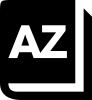
\includegraphics[width=4mm]{icon/definition}
Icône « Book » de 
\href{https://thenounproject.com/dergraph}{Thomas Elbig} de 
\href{https://thenounproject.com}{The noun project}


\includegraphics[width=4mm]{icon/reflexion}
Icône « Thinking » de 
\href{https://thenounproject.com/kukkik_jung/}{Monkik} de 
The noun project

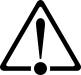
\includegraphics[width=4mm]{icon/attention}
Icône « Attention » de 
\href{https://thenounproject.com/vkvineet}{Vineet Kumar Thakur} de
The noun project


\includegraphics[width=4mm]{icon/fiche}
Icône « Card » de 
\href{https://thenounproject.com/sandorsz}{Alexander Skowalsky} de
The noun project


\includegraphics[width=4mm]{icon/dont}
Icône « Stop » de 
\href{https://thenounproject.com/grega.cresnar}{Gregor Cresnar} de
The noun project


\includegraphics[width=4mm]{icon/java}
Icône « Coffee » de 
\href{https://thenounproject.com/Luis}{Luis Prado} de
The noun project




\vspace{1cm}

\includegraphics[width=25mm]{images/cc-by-sa}

Ce document est mis à disposition selon les termes de la Licence Creative
\\Commons Attribution - Partage dans les Mêmes Conditions 4.0 International.
\\\url{https://creativecommons.org/licenses/by-sa/4.0/deed.fr}

Les autorisations au-delà du champ de cette licence
peuvent être demandées à \texttt{\contact}.


	% =======================================================
% Table des matières
% =======================================================
%\stopcontents[chapters]

\setcounter{tocdepth}{1}
\tableofcontents



	\part{Introduction générale}	
	%----------------------------------------------------------
		% =====================================
\chapter{Résoudre des problèmes}
% =====================================

	\begin{Exergue}
		«~L’algorithmique est le permis de conduire de l’informatique.
		Sans elle, il n’est pas concevable d’exploiter sans risque un ordinateur.~»
		\footnote{[CORMEN e.a., Algorithmique, Paris, Edit. Dunod, 2010, (Cours, 
		exercices et problèmes), p. V] }
	\end{Exergue}

	Ce chapitre a pour but
	de vous faire comprendre ce qu’est une 
	\emph{procédure de résolution de problèmes}.

	\minitoc

	%------------------------------
	\section{La notion de problème}
	%------------------------------
	
		\subsection{Préliminaires~:~utilité de l’ordinateur}
		%---------------------------------------------------
		
			L’ordinateur est une machine. 
			Mais une machine intéressante dans la mesure 
			où elle est destinée d’une part, 
			à nous décharger d’une multitude de tâches peu valorisantes, 
			rébarbatives telles que le travail administratif répétitif, 
			mais surtout parce qu’elle est capable de nous aider, 
			voire nous remplacer, dans des tâches plus ardues 
			qu’il nous serait impossible de résoudre sans son existence 
			(conquête spatiale, prévision météorologique, jeux vidéo\dots).
			
			En première approximation, nous pourrions dire que l’ordinateur est
			destiné à nous remplacer, à faire à notre place (plus rapidement et
			probablement avec moins d’erreurs) un travail nécessaire à la
			résolution de \textbf{problèmes} auxquels nous devons faire face.
			Attention~! Il s’agit bien de résoudre des \textit{problèmes} et non
			des mystères (celui de l’existence, par exemple).  Il faut que la
			question à laquelle nous souhaitons répondre soit \textbf{accessible
			à la raison}.
	
		\subsection{Poser le problème}
		%---------------------------------------------------
		
			Un préalable à l’activité de résolution d’un problème 
			est de bien \textbf{définir} d’abord 
			quel est le problème posé, 
			en quoi il consiste exactement~; 
			par exemple, faire un baba au rhum, 
			réussir une année d’études, 
			résoudre une équation mathématique\dots
			
			Un problème bien posé doit mentionner 
			l’\textbf{objectif à atteindre},
			c’est-à-dire la situation d’arrivée, 
			le but escompté, le résultat attendu. 
			Généralement, tout problème se définit d’abord explicitement
			par ce que l’on souhaite obtenir.
			
			La formulation d’un problème ne serait pas complète 
			sans la connaissance
			\textbf{du cadre dans lequel le problème est posé~:}
			de quoi dispose-t-on, quelles sont les hypothèses de base, 
			quelle est la situation de départ~? 
			Faire un baba au rhum est un problème tout à fait différent 
			s’il faut le faire en plein désert 
			ou dans une cuisine super équipée~! 
			D’ailleurs, dans certains cas, 
			la première phase de la résolution d’un problème 
			consiste à identifier et mettre à sa disposition 
			les éléments nécessaires à sa résolution~:~
			dans notre exemple, 
			ce serait se procurer les ingrédients 
			et les ustensiles de cuisine.
		
			Un problème ne sera véritablement bien spécifié 
			que s’il s’inscrit dans le schéma suivant~:
			
			% Voir si j’en fais un environnement.
			\begin{center}
			\begin{Ovalbox}
				{\textbf{étant donné} [la situation de départ] 
				\textbf{on demande} [l’objectif]}
			\end{Ovalbox}
			\end{center}
		
			Parfois, la première étape dans la résolution d’un problème 
			est de préciser ce problème à partir d’un énoncé flou~:~
			il ne s’agit pas nécessairement d’un travail facile~!
	
			\begin{Emphase}
				\paragraph{Exercice} Un problème flou.\\
				Soit le problème suivant~:~
				«~Calculer la moyenne de nombres entiers.~».\\
				Ce problème est-il bien posé~?\\
				Expliquez pourquoi cet énoncé n'est pas bon. \\
				Proposez un énoncé qui soit acceptable.
			\end{Emphase}
			
			Une fois le problème correctement posé, 
			on passe à la recherche et à la description 
			d’une \textbf{méthode/procédure de résolution}, 
			afin de savoir comment faire 
			pour atteindre l’objectif demandé 
			à partir de ce qui est donné. 
			Le \textbf{nom} donné à une méthode de résolution 
			varie en fonction du cadre dans lequel se pose le problème~:~
			\textit{façon de procéder, mode d’emploi, marche à suivre, 
			guide, patron, modèle, recette de cuisine, 
			méthode ou plan de travail, algorithme mathématique, 
			programme, directives d’utilisation\dots}
	
	%--------------------------------
	\section{Procédure de résolution}
	%--------------------------------
	
		Une \textbf{procédure de résolution} est une description 
		en termes compréhensibles par l’exécutant 
		de la \textbf{marche à suivre} 
		pour résoudre un problème donné.
		
		On trouve beaucoup d’exemples dans la vie courante~:
		recette de cuisine, mode d’emploi d’un GSM, 
		description d’un itinéraire, 
		plan de montage d’un jeu de construction, etc. 
		Il est clair qu’il y a une infinité de rédactions possibles 
		de ces différentes marches à suivre. 
		Certaines pourraient être plus précises que d’autres,
		d’autres par contre pourraient s’avérer exagérément explicatives.		

		Des différents exemples de procédures de résolution 
		se dégagent les caractéristiques suivantes~:	
		\begin{itemize}
		\item 
			toutes ont un \textbf{nom}
		\item 
			elles s’expriment dans un \textbf{langage}
			(français, anglais, dessins\dots)
		\item 
			l’ensemble de la procédure consiste 
			en une \textbf{série chronologique}
			d’instructions ou de phrases (parfois numérotées)
		\item 
			une instruction se caractérise par un ordre, 
			une action à accomplir,
			une \textbf{opération} à exécuter 
			sur les \textbf{données} du problème
		\item 
			certaines phrases justifient ou expliquent ce qui se passe~:~
			ce sont des \textbf{commentaires}.
		\end{itemize}
	
		On pourra donc définir, en première approximation, 
		une procédure de résolution comme un texte, 
		écrit dans un certain langage, 
		qui décrit une suite d’actions à exécuter dans un ordre précis, 
		ces actions opérant sur des objets issus des données du problème.
		
		Traduite en termes informatiques, une telle procédure d'exécutions d'actions
		dans un contexte précis, sera appelée un \textbf{algorithme}. Nous y reviendrons
		et le définirons tout à fait précisément plus loin, dans notre contexte.
	
		\subsection{Chronologie des opérations}
		%--------------------------------------
		
			Pour ce qui concerne l’ordinateur, 
			le travail d’exécution d’une marche à suivre 
			est impérativement \textbf{séquentiel}. 
			C’est-à-dire que les instructions d’une procédure de résolution 
			sont exécutées \textbf{une et une seule fois} 
			dans l’ordre où elles apparaissent.
			Cependant certains artifices d’écriture 
			permettent de \textbf{répéter} l’exécution d’opérations 
			ou de la \textbf{conditionner}
			(c’est-à-dire de choisir si l’exécution aura lieu ou non 
			en fonction de la réalisation d’une condition).
	
		\subsection{Les opérations élémentaires}
		%---------------------------------------
		
			Dans la description d’une marche à suivre, 
			la plupart des opérations sont introduites par un \textbf{verbe}
			(\textit{remplir}, \textit{verser, prendre, peler}, etc.). 
			L’exécutant ne pourra exécuter une action que s’il la comprend~:
			cette action doit, pour lui, être une action élémentaire, 
			une action qu’il peut réaliser 
			sans qu’on ne doive lui donner des explications complémentaires. 
			Ce genre d’opération élémentaire est appelée \textbf{primitive}.
			
			Ce concept est évidemment relatif 
			à ce qu’un exécutant est capable de réaliser. 
			Cette capacité, il la possède d’abord 
			parce qu’il est \textbf{construit} d’une certaine façon 
			(capacité innée). 
			Ensuite parce que, par construction aussi, 
			il est doté d’une faculté d’\textbf{apprentissage} 
			lui permettant d’assimiler, petit à petit, 
			des procédures non élémentaires qu’il exécute souvent. 
			Une opération non élémentaire 
			pourra devenir une primitive un peu plus tard.
			
		\subsection{Les opérations bien définies}
		%----------------------------------------
		
			Il arrive de trouver dans certaines marches à suivre 
			des opérations qui peuvent dépendre d’une certaine manière 
			de l’appréciation de l’exécutant. 
			Par exemple, dans une recette de cuisine nous pourrions lire~:~
			\textit{ajouter} \textbf{\textit{un peu}} 
			\textit{de vinaigre, saler et poivrer} 
			\textbf{\textit{à volonté}}, \textit{laisser cuire une} 
			\textbf{\textit{bonne}}
			\textit{ heure dans un four}
			\textbf{\textit{bien}} \textit{chaud, etc.}
			
			Des instructions floues de ce genre 
			sont dangereuses à faire figurer dans une bonne marche à suivre 
			car elles font appel à une appréciation arbitraire de l’exécutant. 
			Le résultat obtenu risque d’être imprévisible 
			d’une exécution à l’autre. 
			De plus, les termes du type \textit{environ, beaucoup, pas trop} 
			et \textit{à peu près} sont intraduisibles 
			et proscrites au niveau d’un langage informatique~!%
			\footnote{%
				Toute personne intéressée découvrira 
				dans la littérature spécialisée 
				que même les procédures de génération de nombres aléatoires
				sont elles aussi issues d’algorithmes mathématiques 
				tout à fait déterministes.
			}
			
			Une \textbf{opération bien définie} 
			est donc une opération débarrassée
			de tout vocabulaire flou 
			et dont le résultat est \textbf{entièrement prévisible}. 
			Des versions «~bien définies~» des exemples ci-dessus
			pourraient être~:~
			\textit{ajouter 2~cl de vinaigre, ajouter 5~g de sel
			et 1~g de poivre, 
			laisser cuire 65~minutes dans un four chauffé à 220\degre{}C, etc.}
	
			Afin de mettre en évidence la difficulté d’écrire une marche
			à suivre claire et non ambigüe, l’expérience suivante a été menée et
			vous pouvez la reproduire.
	
			\begin{Emphase}
				\paragraph{Expérience.} Le dessin.
				
				Cette expérience s’effectue en groupe.
				Le but est de faire un dessin 
				et de permettre à une autre personne, 
				qui ne l’a pas vu, 
				de le reproduire fidèlement, 
				au travers d’une «~marche à suivre~».
	
				\begin{enumerate}
				\item
					Chaque personne prend une feuille de papier et 
					y dessine quelque chose en quelques traits précis. 
					Le dessin ne doit pas être trop compliqué~; 
					on ne teste pas ici vos talents de dessinateur~! 
					(ça peut être une maison, une voiture\dots)
				\item
					Sur une \textbf{autre} feuille de papier, 
					chacun rédige des instructions permettant de 
					reproduire fidèlement son propre dessin. 
					Attention~! Il est important de ne
					\textbf{jamais faire référence à la signification du dessin}. 
					Ainsi, on peut écrire~:~«~dessine un rond~» 
					mais certainement pas~:~«~dessine une roue~».
				\item
					Chacun cache à présent son propre dessin et échange 
					sa feuille d’instructions avec celle de quelqu’un d’autre.
				\item
					Chacun s’efforce ensuite 
					de reproduire le dessin d’un autre 
					en suivant \textbf{scrupuleusement} 
					les instructions indiquées sur la feuille reçue en échange, 
					\textbf{sans tenter d’initiative} 
					(par exemple en croyant avoir compris ce
					qu’il faut dessiner).
				\item
					Nous examinerons enfin les différences 
					entre l’original et la reproduction 
					et nous tenterons de comprendre 
					pourquoi elles se sont produites 
					(par imprécision des instructions 
					ou par mauvaise interprétation de celles-ci 
					par le dessinateur\dots)
				\end{enumerate}
			\end{Emphase}
	
			\marginicon{reflexion}
			Quelles réflexions cette expérience vous inspire-t-elle~?
			Quelle analogie voyez-vous 
			avec une marche à suivre donnée à un ordinateur~?
	
			Dans cette expérience, 
			nous imposons que la «~marche à suivre~» 
			ne mentionne aucun mot expliquant le sens du dessin 
			(mettre «~rond~» et pas «~roue~» par exemple). 
			Pourquoi, à votre avis, avons-nous imposé cette contrainte~?
	
		\subsection{Opérations soumises à une condition}
		%-----------------------------------------------
		
			En français, 
			l’utilisation de conjonctions ou locutions conjonctives 
			du type \textit{si}, \textit{selon que}, \textit{au cas où}\dots{}
			présuppose la possibilité 
			de ne pas exécuter certaines opérations 
			en fonction de certains événements. 
			D’une fois à l’autre, 
			certaines de ses parties seront ou non exécutées.
			
			\textbf{Exemple~:}~
			Si la viande est surgelée, 
			la décongeler à l’aide du four à micro-ondes.
	
		\subsection{Opérations à répéter}
		%--------------------------------
		
			De la même manière, 
			il est possible d’exprimer en français une exécution
			répétitive d’opérations en utilisant les mots \textit{tous},
			\textit{chaque}, \textit{tant que}, \textit{jusqu’à ce que},
			\textit{chaque fois que}, \textit{aussi longtemps que}, 
			\textit{faire x fois}\dots 
			
			Dans certains cas, 
			le nombre de répétitions est connu à l’avance
			(\textit{répéter 10 fois}) 
			ou déterminé par une durée 
			(\textit{faire cuire pendant 30 minutes}) 
			et dans d’autres cas il est inconnu.
			Dans ce cas, la fin de la période de répétition 
			d’un bloc d’opérations dépend alors 
			de la réalisation d’une condition 
			(\textit{lancer le dé jusqu’à ce qu’il tombe sur 6}, 
			\textit{faire chauffer jusqu’à évaporation complète}\dots). 
			
			En informatique, lorsqu'il y a répétition organisée, on parle de 
			\textbf{boucle}. On en retrouve beaucoup, sous différentes formes,
			dans les codes informatiques.
			
			L'exemple ci-dessous permet d'illustrer le danger de boucle infinie,
			due à une mauvaise formulation de la condition d’arrêt.  Si l'on
			demande de \textit{lancer le dé — de 6 faces — jusqu’à ce que la
			valeur obtenue soit 7}, une personne dotée d’intelligence comprend
			que la condition est impossible à réaliser, mais un robot appliquant
			cette directive à la lettre lancera le dé perpétuellement.
	
		\subsection{À propos des données}
		%--------------------------------
		
			Les types d’objets figurant 
			dans les diverses procédures de résolution
			sont fonction du cadre 
			dans lequel s’inscrivent ces procédures, 
			du domaine d’application de ces marches à suivre. 
			Par exemple, pour une recette de cuisine, 
			ce sont les ingrédients. 
			Pour un jeu de construction ce sont les briques.
			
			L’ordinateur, quant à lui, manipule principalement
			des données numériques et textuelles. 
			Nous verrons plus tard 
			comment on peut combiner ces données élémentaires 
			pour obtenir des données plus complexes.
	
	%-------------------
	\section{Ressources}
	%-------------------
	
		Pour prolonger votre réflexion sur le concept d’algorithme
		nous vous proposons quelques ressources en ligne~:
		\begin{itemize}
		\item
			\href{https://www.youtube.com/watch?v=hG9Jty7P6Es}
			{Les Sépas 18 - Les algorithmes}
		\item
			\href{https://www.youtube.com/watch?v=deI0GV5sWTY}
			{Les Sépas 11 - Un bug}
		\item
			\href{https://pixees.fr/?p=446}
			{Le crépier psycho-rigide comme algorithme}
		\item
			\href{https://pixees.fr/?p=450}
			{Le baseball multicouleur comme algorithme}
		\item
			\href{https://pixees.fr/?p=443}
			{Le jeu de Nim comme algorithme}
		\end{itemize}
		

		% ========================================================================
\chapter{Les algorithmes et les programmes}
\label{algoprog}
% ========================================================================

	Notre but étant de faire de l’informatique, 
	il convient de restreindre notre étude 
	à des notions plus précises, plus spécialisées, 
	gravitant autour de la notion de 
	\textit{traitement automatique de l’information}.
	Voyons ce que cela signifie.

	\minitoc

	%----------------------------------
	\section{Algorithmes et programmes}
	%----------------------------------
	
		Décrivons la différence entre un algorithme et un programme
		et comment un ordinateur peut exécuter un programme.
	
		\subsection{Algorithme}
		%----------------------
		
			Un algorithme appartient au vaste ensemble 
			des \textit{marches à suivre}.
	
			\marginicon{definition}\index{algorithme}
			\textbf{Algorithme}~:~
			Procédure de résolution d’un problème 
			contenant des opérations bien définies 
			portant sur des informations, 
			s’exprimant dans une séquence définie sans ambigüité, 
			destinée à être traduite dans un langage de programmation.
		
			Comme toute marche à suivre, un algorithme doit s’exprimer dans un
			certain langage~—~ à priori le langage naturel~—~ mais il
			y a d’autres possibilités~:~ ordinogramme, arbre programmatique,
			pseudo-code…

			L'algorithme est destiné à être compris par une personne et à être
			traduit — ce qui n'est pas immédiat — en un programme. 

			\textbf{Exemple simple}

			\begin{Emphase}
				\paragraph{} Calculer la circonférence d'un cercle.
			\end{Emphase}

			Un algorithme en \textbf{langage naturel} pourrait être: en
			connaissant le rayon, le calcul de la circonférence se fait grâce
			à  $$p = 2\pi r$$

			En utilisant un \textbf{organigramme} l'algorithme peut se décrire
			comme suit (et nous y reviendrons plus longuement plus tard):

			\begin{center}
			\begin{tikzpicture}[node distance=2cm]
			\node (start) [startstop] {Circonférence d'un cercle en connaissant 
				$r$};
			\node (pro1) [process, below of=start] {$p = 2\pi r$};
			\draw [arrow] (start) -- (pro1);
			\node (stop) [startstop, below of=pro1] {Stop};
			\draw [arrow] (pro1) -- (stop);
			\end{tikzpicture}
			\captionof{Organigramme}{Illustration d'un organigramme}
			\end{center}

			En \textbf{pseudo-code} cette fois, l'algorithme aurait l'allure
			suivante:
			
			\begin{pseudocode}
				\Algo{circleCircumference}{\Par{radius}{real}}{real}
					\Return 2 $\pi$ ~radius
				\EndAlgo
			\end{pseudocode}
			
			
	
		\subsection{Programme}
		%---------------------
		
			\marginicon{definition}\index{programme}
			Un \textbf{programme} n’est rien d’autre 
			que la représentation d’un algorithme 
			dans un langage plus technique compris par un ordinateur 
			(par exemple~:~Assembleur, Cobol, Java, C++\dots). 
			Ce type de langage est appelé 
			\textbf{langage de programmation}.
			
			Écrire un programme correct suppose donc 
			la parfaite connaissance du langage de programmation 
			et de sa \textbf{syntaxe}, 
			qui est en quelque sorte la grammaire du langage. 
			Mais ce n’est pas suffisant~! 
			Puisque le programme est la représentation d’un algorithme, 
			il faut que celui-ci soit correct pour que le programme le soit. 
			Un programme correct résulte donc d’une démarche logique correcte 
			(algorithme correct) 
			et de la connaissance de la syntaxe d’un langage de programmation.
			La syntaxe d'un langage est — très — précise. 
			
			\textbf{%
			Il est donc indispensable d’élaborer des algorithmes corrects 
			avant d’espérer concevoir des programmes corrects.
			}

			\textbf{Un exemple simple (suite)}

			En Java, le programme aurait l'allure suivante mais ne serait pas
			utilisable en l'état. Il lui manque une méthode principale. Nous
			y reviendrons: 

			\begin{java}
public class CircleCircumference{
	public static double circleCircumference(double radius){
		return 2 * Math.PI * radius;
	}
}
			\end{java}

	
		\subsection{Les constituants principaux de l’ordinateur}
		%-------------------------------------------------------
		
			Les constituants d’un ordinateur 
			se divisent en \textbf{hardware} (matériel) 
			et \textbf{software d’exploitation} (logiciel).
			
			Le \textbf{hardware} est constitué 
			de l’ordinateur proprement dit 
			et regroupe les entités suivantes~:
	
			\begin{itemize}
			\item
				\textbf{l’organe de contrôle~:}~
				c’est le cerveau de l’ordinateur. 
				Il est l’organisateur, 
				le contrôleur suprême de l’ensemble. 
				Il assume l’enchainement des opérations élémentaires. 
				Il s’occupe également d’organiser l’exécution effective
				de ces opérations élémentaires reprises dans les programmes.
			\item
				\textbf{l’organe de calcul~:}~
				c’est le calculateur 
				où ont lieu les opérations arithmétiques ou logiques. 
				Avec l’organe de contrôle, 
				il constitue le \textbf{processeur} 
				ou \textbf{unité centrale}.
			\item
				\textbf{la mémoire centrale~:}~
				dispositif permettant de mémoriser,
				pendant le temps nécessaire à l’exécution, 
				les programmes et certaines données pour ces programmes.
			\item
				\textbf{les unités d’échange avec l’extérieur~:} 
				dispositifs permettant à l’ordinateur de recevoir 
				des informations de l’extérieur 
				(unités de lecture telles que clavier, souris, écran tactile\dots) 
				ou de communiquer des informations vers l’extérieur 
				(unités d’écriture telles que écran, imprimantes, signaux sonores\dots).
			\item
				\textbf{les unités de conservation à long terme~:}~
				ce sont les mémoires auxiliaires 
				(disques durs, CD ou DVD de données, clés USB\dots) 
				sur lesquelles sont conservées les procédures (programmes) 
				ou les informations résidentes dont le volume 
				ou la fréquence d’utilisation ne justifient pas 
				la conservation permanente en mémoire centrale.
			\end{itemize}
			
			Le \textbf{software d’exploitation} 
			est l’ensemble des procédures (programmes) 
			s’occupant de la gestion du fonctionnement 
			d’un système informatique 
			et de la gestion de l’ensemble des ressources de ce système 
			(le matériel –~les programmes~– les données). 
			Il contient notamment des logiciels de traduction 
			permettant d’obtenir un programme écrit en langage machine 
			(langage technique qui est le seul que l’ordinateur 
			peut comprendre directement, c’est-à-dire exécuter) 
			à partir d’un programme écrit en langage de programmation 
			plus ou moins «~évolué~» 
			(c’est-à-dire plus ou moins proche du langage naturel).
	
		\subsection{Exécution d’un programme}
		%------------------------------------
		
			Isolons (en les simplifiant) deux constituants essentiels de
			l’ordinateur afin de comprendre ce qu'il se passe quand un
			ordinateur exécute un programme.  D’une part, la mémoire contient le
			programme et les données manipulées par ce programme.  D’autre part,
			le processeur va «~exécuter~» ce programme.
	
			\begin{tabular}{m{0.46\linewidth}m{0.46\linewidth}}
				\begin{center}
				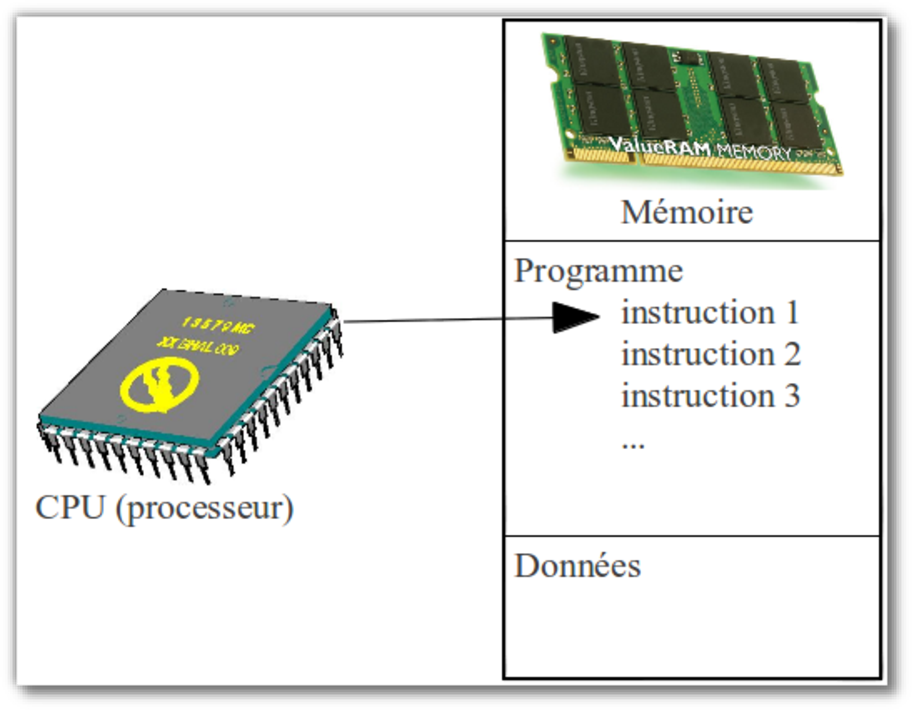
\includegraphics[width=0.45\textwidth]{images/intro-schema-ordi}
				\end{center}
			&
				\textbf{Comment fonctionne le processeur~?}
		
				De façon très simplifiée, les étapes suivantes ont lieu~:
		
				\medskip
				\begin{flushleft}
				\begin{enumerate}
				\item Le processeur lit l’instruction courante.
				\item Il exécute cette instruction. Cela peut amener à manipuler les données.
				\item L’instruction suivante devient l’instruction courante.
				\item On revient au point 1.
				\end{enumerate}
				\end{flushleft}
			\\
			\end{tabular}
	
			\textbf{%
			Nous voyons bien qu’il s’agit d’un travail automatique 
			ne laissant aucune place à l’initiative~!
			}
	
	%------------------------------------------------
	\section{Les phases d’élaboration d’un programme}
	%------------------------------------------------
	
		Voyons pour résumer un schéma \textbf{simplifié} des différentes phases
		nécessaires au développement d'un programme.
	
		\begin{tabular}{m{0.20\linewidth}m{0.75\linewidth}}
		{\sffamily
		\begin{tikzpicture}
			\matrix [row sep = 2em] {
			 \node[draw, rounded corners, thick] (P1) {Analyse}; \\
			 \node[draw, rounded corners, thick] (P2) {Algorithmes}; \\
			 \node[draw, rounded corners, thick] (P3) {Programmation}; \\
			 \node[draw, rounded corners, thick] (P4) {Tests}; \\
			 \node[draw, rounded corners, thick] (P5) {Livraison}; \\
			};
			\draw[->, thick] (P1) to (P2);
			\draw[->, thick] (P2) to (P3);
			\draw[->, thick] (P3) to (P4);
			\draw[->, thick] (P4) to (P5);
		\end{tikzpicture}
		}
		&
		\begin{itemize}
		\item 
			Lors de \textbf{l’analyse}, 
			le problème doit être compris et clairement précisé. 
			Vous aborderez cette phase dans le cours d’analyse.
		\item
			Une fois le problème analysé, 
			et avant de passer à la phase de programmation, 
			il faut réfléchir à l’\textbf{algorithme} 
			qui va permettre de résoudre le problème. 
		\item
			On peut alors \textbf{programmer} cet algorithme 
			dans le langage de programmation choisi~;~Java, 
			Cobol, Assembleur, Python \dots
		\item
			Vient ensuite la phase de \textbf{tests} 
			qui ne manquera pas de montrer qu’il subsiste des problèmes 
			qu’il faut encore corriger. 
			(Vous aurez maintes fois l’occasion 
			de vous en rendre compte lors des séances de laboratoire)
		\item
			Le produit sans bug (connu) peut être \textbf{mis en application}
			ou \textbf{livré} à la personne 
			qui vous en a passé la commande.
		\end{itemize}
		\\
		\end{tabular}
		
		Notons que ce processus n’est pas linéaire. À chaque phase, on pourra
		détecter des erreurs, imprécisions ou oublis des phases précédentes et
		revenir en arrière. Un problème peut être amélioré, complexifié, modifié
		ou étendu. 

		Par exemple~: Imaginons que je veuille préparer un repas pour mes
		invités et invitées. Je désire leur proposer une lasagne et décide de
		suivre une recette. À la dernière minute, j'apprend que l'une des
		personne invitée est allergique au lait. Plusieurs choix s'offrent à moi~: 

		\begin{itemize}
			\item je modifie ma recette et remplace le lait par du lait de soja;
			\item je change de plat;
			\item je le notifie qu'il ou elle n'est plus le bienvenu·e ou qu'il 
				recevra une tartine.
		\end{itemize}

	
		\textbf{Pourquoi passer par la phase «~algorithmique~» 
			et ne pas directement passer à la programmation~?}
		
		Voilà une question que vous ne manquerez pas de vous poser 
		pendant votre apprentissage cette année. 
		Apportons quelques éléments de réflexion.
	
		\begin{itemize}
		\item
			Passer par une phase «~algorithmique~» 
			permet de séparer deux difficultés~:~
			quelle est la marche à suivre~? 
			Et comment l’exprimer dans le langage de programmation choisi~? 
			Le langage que nous allons utiliser en algorithmique 
			est plus souple et plus général que le langage Java
			par exemple (où il faut être précis au «~;~» près).
		\item
			De plus, un algorithme écrit facilite le dialogue 
			dans une équipe de développement. 
			«~J’ai écrit un algorithme 
			pour résoudre le problème qui nous occupe. 
			Qu’en pensez-vous~? Pensez-vous qu’il est correct~?
			Avez-vous une meilleure idée~?~». 
			L’algorithme est plus adapté à la communication car plus lisible.
		\item
			Enfin, si l’algorithme est écrit, 
			il pourra facilement être traduit
			dans n’importe quel langage de programmation. 
			La traduction d’un langage de programmation à un autre
			est un peu moins facile 
			à cause des particularités propres à chaque langage.
		\end{itemize}
	
		Bien sûr, cela n’a de sens que si le problème présente
		une réelle difficulté algorithmique. 
		Certains problèmes (en pratique, certaines parties de problèmes) 
		sont suffisamment simples pour être directement programmés. 
		Mais qu’est-ce qu’un problème simple~? 
		Cela va évidemment changer tout au long de votre apprentissage. 
		Un problème qui vous paraitra difficile en début d’année 
		vous paraitra (enfin, il faut l’espérer~!) 
		une évidence en fin d’année.
	
	%-------------------
	\section{Conclusion}
	%-------------------
	
		L’informatisation de problèmes 
		est un processus essentiellement dynamique, 
		contenant des allées et venues constantes 
		entre les différentes étapes. 
		Codifier un algorithme dans un langage de programmation quelconque 
		n’est certainement pas la phase la plus difficile de ce processus. 
		Par contre, élaborer une démarche logique de résolution 
		d’un problème est probablement plus complexe.
		
		Le but de ce premier cours de \textbf{développement} est de mêler 
		l'apprentissage des algorithmes et du langage Java comme premier 
		langage. 
		
		Nous tenterons~:
	
		\begin{itemize}

		\item
			de définir une bonne démarche d’élaboration d’algorithmes
			(apprentissage de la \textbf{logique} de programmation)~;
		\item
			comprendre et apprendre les algorithmes classiques 
			qui ont fait leurs preuves.
			Pouvoir les utiliser en les adaptant 
			pour résoudre nos problèmes concrets.
		\item
			traduire ces algorithmes en langage Java et les « faire tourner »,
			c'est-à-dire les implémenter sur une machine~; éditer le code, le
			compiler, l'exécuter…
		
		\end{itemize}
	
		Le tout devrait avoir pour résultat l’élaboration 
		de \textit{bons programmes}, 
		c’est-à-dire \textit{des programmes dont il est facile de
		se persuader qu’ils sont corrects} et des programmes dont la
		maintenance est la plus aisée possible. 
		Dans ce sens, ce cours est bien un premier cours de développement.
		
		Les matières non traitées dans cette première approche du développement 
		le seront, d'abord dans le cours de Développement II (DEV2) et ensuite,
		Développement III, IV… en fonction du cursus. 

	%-------------------
	\section{Ressources}
	%-------------------
	
		Pour prolonger votre réflexion 
		sur les notions vues dans ce chapitre, 
		nous vous proposons quelques ressources en ligne~:
		\begin{itemize}
		\item
			C'est pas sorcier~! 
			\href{https://www.youtube.com/watch?v=c96KP5jZVYk}
			{Ordinateur, tout un programme}
		\end{itemize}


	\part{Les bases de l'algorithmique et de la programmation}
	%----------------------------------------------------------
		%==============================
\chapter{Spécifier le problème}
%==============================

	Comme nous l’avons dit, 
	un problème ne sera véritablement bien spécifié 
	que s’il s’inscrit dans le schéma suivant~:
		
	\medskip
	\begin{center}
	\begin{Ovalbox}
		{\textbf{étant donné} [les données] 
		\textbf{on demande} [résultat]}
	\end{Ovalbox}
	\end{center}
	\medskip
	
	La première étape dans la résolution d’un problème est de
	préciser ce problème à partir de l’énoncé,
	c-à-d de déterminer et préciser les données et le résultat.
	
	\minitoc

	%----------------------------------------------
	\section{Déterminer les données et le résultat}
	%----------------------------------------------
	
		La toute première étape est de parvenir à extraire
		d’un énoncé de problème, quelles sont les données
		et quel est le résultat attendu%
		\footnote{%
			Plaçons-nous pour le moment dans le cadre
			de problèmes où il y a exactement un résultat.%
		}. Dans la suite, nous utiliserons un exemple très simple afin 
		d'illustrer les concepts qui nous intéressent. 
	
		\clearpage
		\vspace{1cm}
	
		\begin{Emphase}
			\paragraph{Exemple.}
			Soit l’énoncé suivant~:
			\og
				Calculer la surface d’un rectangle 
				à partir de sa longueur et sa largeur
			\fg.
			
			Quelles sont les données~? Il y en a deux~:	
			\begin{itemize}
				\item la longueur du rectangle~;
				\item sa largeur.
			\end{itemize}
		
			Quel est le résultat attendu~? la surface du rectangle.
		\end{Emphase}
		
	%----------------------------------------------
	\section{Les noms}\index{noms}
	%----------------------------------------------
	
		Pour identifier clairement chaque \textbf{donnée}
		et pouvoir y faire référence dans le futur algorithme
		et dans le programme
		nous devons lui attribuer un \textbf{nom}%		
		\footnote{%
				Dans ces notes, nous nous efforcerons de choisir des noms en 
				anglais,
				mais vous pouvez très bien choisir
				des noms français si vous ne vous sentez pas encore suffisamment 
				à l'aise avec l'anglais.
		}.
		Il est important de bien choisir les noms. 
		Le but est de trouver un nom qui soit suffisamment court,
		tout en restant explicite et ne prêtant pas à confusion.
		
	
		\begin{Emphase}
			\paragraph{Exemple.}	
			Quel nom choisir pour la longueur d’un rectangle~?
	
			On peut envisager les noms suivants~:
			\begin{itemize}
			\item
				\pc{length} est probablement le plus approprié.
			\item
				\pc{rectangleLength} peut se justifier
				pour éviter toute ambigüité avec une autre longueur.
			\item
				\pc{len} peut être admis
				si le contexte permet de comprendre immédiatement
				l’abréviation.
			\item
				\pc{l} est à proscrire car pas assez explicite.
			\item
				\pc{theLengthOfMyRectangle} est inutilement long. 
			\item
				\pc{foo} (truc en anglais) ou \pc{tmp} ne sont pas de bons choix
				car ils n’ont aucun lien avec la donnée.
			\end{itemize}
		\end{Emphase}

		Les noms donnés à chaque donnée seront directement associés à une 
		\textbf{variable} lorsque l'algorithme sera traduit en un programme dans 
		un langage de programmation. 
		
		\marginicon{definition}\index{variable} \textbf{Variable}~:~ Emplacement
		mémoire nommé pouvant contenir une valeur. Cette valeur peut être
		remplacée par une autre — elle est variable — au fil de l'exécution du
		programme. 
		
		Nous allons également donner un \textbf{nom à l’algorithme}
		de résolution du problème.
		Cela permettra d’y faire référence dans les explications
		mais également de l’utiliser dans d’autres algorithmes.
		Généralement, un nom d’algorithme est~:
		\begin{itemize}
		\item soit un verbe indiquant ce que fait l’algorithme~;
		\item soit un nom indiquant le résultat fourni.	
		\end{itemize}
	
		\clearpage
		\begin{Emphase}
			\paragraph{Exemple.}	
			Quel nom choisir pour l’algorithme 
			qui calcule la surface d’un rectangle~?
	
			On peut envisager 
			le verbe \pc{computeRectangleArea}
			ou le nom \pc{rectangleArea} (notre préféré).
			On pourrait aussi simplifier en \pc{area}
			s’il est évident que le problème traite des rectangles.
		\end{Emphase}
	
		Les noms donnés aux algorithmes deviendront généralement les noms des
		programmes lorsque ces algorithmes seront implémentés. 

		Notons que les langages de programmation imposent certaines limitations
		(parfois différentes d’un langage à l’autre) ce qui peut nécessiter une
		modification du nom lors de la traduction de l’algorithme en un
		programme. À chaque langage de programmation sont également associées
		des \textbf{conventions d'écriture} que les développeurs respectent.
		Bien que nous y reviendrons plus en détail dans la section
		\ref{lisibilite}, notons déjà que la simple convention de nom de méthode
		change d'un langage à l'autre. 
		
		Par exemple pour \textit{rectangle area}, nous utiliserons
		\pc{rectangleArea} en langage Java mais \pc{rectangle\_area} en langage
		C, C++ et Python. 

	%----------------------------------------------
	\section{Les types}\index{types}
	%----------------------------------------------
		
		Nous allons également attribuer un \textbf{type} à chaque donnée ainsi
		qu’au résultat.  Le \textbf{type} décrit la nature de son contenu,
		quelles valeurs elle peut prendre.
		
		Certains langages imposent et vérifient le type de chaque variable tandis
		que d'autres non. En Java, chaque variable et chaque donnée ont un type. 
		
		Dans un premier temps, nous utiliserons ces \textbf{types}
		\footnote{Écrire ces différents types en français n'est pas une 
		faute. Dans ces notes nous utiliserons l'anglais}~:
		
		\begin{center}
			\begin{tabular}[t]{|p{1.4cm}|p{8cm}|}
				\hline
				\rowcolor{black!40}
				\color{white}\bf\large Type & \\
				\hline
				\pc{int} & pour les nombres entiers\\
				\pc{double} & pour les nombres réels\\
				\pc{String}
						\footnote{Notez la majuscule, indispensable en Java} 
						& \makecell[tl]{
							pour les chaines de caractères, les textes\\
							par exemple~:\\
							\hspace{1cm}\pc{"Bonjour"},\\
							\hspace{1cm}\pc{"Bonjour le monde !"},\\
							\hspace{1cm}\pc{"a"}, \pc{""}\dots
						}
					\\
				\pc{boolean} & quand la valeur 
			ne peut être que \pc{true} (vrai) ou \pc{false} (faux)\\
			\hline
			\end{tabular}
		\end{center}


		\clearpage
		\begin{Emphase}
			\paragraph{Exemples.}	
			\begin{itemize}
			\item Pour la longueur, la largeur et la surface d’un rectangle, 
				on prendra un réel (le type \pc{double}).
			\item Pour le nom d’une personne, on choisira une chaine de caractère
				(le type \pc{String}).
			\item Pour l’âge d’une personne, un entier est indiqué (\pc{int}).
			\item Pour décrire si un étudiant est doubleur ou pas, un booléen 
				(\pc{boolean}) est adapté.
			\item Pour représenter un mois, on préférera souvent un entier
				donnant le numéro du mois (par ex: 3 pour le mois de mars)
				plutôt qu’une chaine (par ex: "mars")
				car les manipulations, les calculs seront plus simples.
			\end{itemize}
		\end{Emphase}
	
		\subsection{Il n’y a pas d’unité}
		%-----------------------------------------
	
			Un type numérique indique que les valeurs possibles seront
			des nombres. Il n’y a là aucune notion d’unité.
			Ainsi, la longueur d’un rectangle, un réel, 
			peut valoir $2.5$ mais certainement pas $2.5$\,$cm$.
			Si cette unité a de l’importance,
			il faut la spécifier dans le nom de la donnée ou en commentaire.
			
			\begin{Emphase}
				\paragraph{Exemple.}
				Faut-il préciser les unités 
				pour les dimensions d’un rectangle~?
				
				Si la longueur d’un rectangle vaut $6$, 
				on ne peut pas dire s’il s’agit de centimètres, 
				de mètres ou encore de kilomètres.
				Pour notre problème de calcul de la surface,
				ce n’est pas important~;
				la surface n’aura pas d’unité non plus.

				Notre seule contrainte est que la longueur et la largeur soient
				exprimées dans la même unité.
				
				Si, par contre, 
				il est important de préciser que la longueur
				est donnée en centimètres,
				on pourrait l’expliciter en la nommant
				\pc{lengthCm}.	
			\end{Emphase}
	
		\subsection{Préciser les valeurs possibles}
		%-----------------------------------------
		
			Nous aurions pu introduire un seul type numérique
			mais nous avons choisi de distinguer les entiers et les réels.
			Pourquoi~?
			Préciser qu’une donnée ne peut prendre que des valeurs entières
			(par exemple dans le cas d’un numéro de mois)
			aide le lecteur à mieux la comprendre.
			Nous allons aussi pouvoir définir des opérations propres aux entiers
			(le reste d’une division par exemple).
			Enfin, pour des raisons techniques,
			beaucoup de langages font cette distinction.
			
			Même ainsi, le type choisi n’est pas toujours assez précis.
			Souvent, la donnée ne pourra prendre que certaines valeurs.
			
			\clearpage
			\begin{Emphase}
				\paragraph{Exemples.}	
				\begin{itemize} 
				\item Un âge est un entier qui ne peut pas être négatif.
				\item Un mois est un entier compris entre 1 et 12.
				\end{itemize}
			\end{Emphase}
			
			Ces précisions pourront être données en commentaire
			pour aider à mieux comprendre le problème et sa solution.
	
		\subsection{Le type des données complexes}
		%-----------------------------------------
		
			Parfois, aucun des types disponibles ne permet de représenter 
			la donnée.
			Il faut alors la décomposer.
			
			\begin{Emphase}
				\paragraph{Exemple.}	
				Quel type choisir 
				pour la date de naissance d’une personne~?
				
				On pourrait la représenter dans une chaine 
				(par ex: "17/3/1985")
				mais cela rendrait difficile le traitement, les calculs
				(par exemple, déterminer le numéro du mois).
				Le mieux est sans doute de la décomposer en trois parties~: 
				le jour, le mois et l’année, tous des entiers.
			\end{Emphase}
			
			Plus tard, vous verrez qu’il est possible de définir de nouveaux
			types de données grâce aux \emph{structures} pour les algorithmes et
			aux \emph{classes} pour les langages orientés objets tels que Java. 
			
			Il sera alors possible de définir et utiliser un type \pc{Date}
			et il ne sera plus nécessaire de décomposer une date en trois
			morceaux bien que le type sera bien entendu composé de trois valeurs.

	
		\subsection{Exercice}
		%----------------------------------------------
		
			Quel(s) type(s) de données utiliseriez-vous pour représenter~:
			\begin{itemize}
				\item le prix d’un produit en grande surface~;
				\item la taille de l’écran de votre ordinateur~;
				\item votre nom~;
				\item votre adresse~;
				\item le pourcentage de remise proposé pour un produit~;
				\item une date du calendrier~;
				\item un moment dans la journée~?
			\end{itemize}
			
	%----------------------------------------------
	\section{Résumés}
	%----------------------------------------------
	
		Toutes les informations déjà collectées sur le problème
		peuvent être résumées. 
		
		\subsection{Résumé graphique}
		
		Représentation graphique du problème.
	
		\begin{Emphase}
			\paragraph{Exemple.}
			Pour le problème, de la surface du rectangle, 
			on fera le schéma suivant~:
			
			\center\flowalgodd{longueur (réel positif)}
			{largeur (réel positif)}{surfaceRectangle}{réel}	
		\end{Emphase}

		\subsection{Résumé textuel}

		Résumé textuel du problème, indiquant clairement les données et les 
		résultats recherchés. 

		\begin{Emphase}
			\paragraph{Exemple.}
			\begin{tabular}[t]{|>{\columncolor{black!40}}r|l|}
				\hline
				\textbf{Données} & \makecell[tl]{
					longueur (un réel positif)\\
					largeur (un réel positif)
				}\\
				\hline
				\textbf{Résultat} & la surface du rectangle\\
				\hline
			\end{tabular}
		\end{Emphase}
		
	%----------------------------------------------
	\section{Exemples numériques}
	%----------------------------------------------
	
		Une dernière étape pour vérifier que le problème
		est bien compris est de donner quelques exemples numériques.
		Il est possible de les spécifier en français, 
		via un graphique ou via une notation compacte.

		\begin{Emphase}
			\paragraph{Exemples.}
			Voici différentes façons de présenter des exemples numériques
			pour le problème de calcul de la surface d’un rectangle~:
			\begin{itemize}
			\item En français~: 
				si la longueur du rectangle vaut 3 et sa largeur vaut 2, 
				alors sa surface vaut 6.			
			\item Via un schéma~:	
				\begin{center}
					\flowalgodd{length (3)}{width (2)}{rectangleArea}{6}
				\end{center}
			\item En notation compacte~:
				\pc{rectangleArea(3, 2)} donne/vaut $6$.
			\end{itemize}
		\end{Emphase}
	

		%========================================================
\chapter{Premiers algorithmes}
\label{premalgos}
%==========================================================

	Dans le chapitre précédent, vous avez appris à analyser un problème et
	à clairement le spécifier.  Il est temps d’écrire des solutions.  Pour cela,
	nous allons devoir trouver comment passer des données au résultat et
	l’exprimer dans un langage compris de tous.
	
	En fonction de la difficulté du problème et de notre sensibilité, nous
	pouvons représenter un algorithme de plusieurs manières; en langage naturel
	(en français ou en 	anglais), en pseudocode ou avec un organigramme\ldots
	Dans ce chapitre, nous présenterons les algorithmes en langage naturel, en
	pseudocode, avec un organigramme et en langage Java. 

	Dans la suite du cours, nous nous contenterons de les écrire en langage Java. 

	\newpage
	\minitoc
	\newpage
	
	%================================================
	\section{Exercice résolu~: un problème simple}
	\label{exerciceresolu}
	%================================================
	
		%===================================
		\subsection{Trouver l’algorithme}
		%=================================

			Illustrons notre propos sur l’exemple qui a servi de fil conducteur
			tout au long du chapitre précédent.  Rappelons l’énoncé et l’analyse
			qui en a été faite.
			
			\begin{Emphase}
				\paragraph{Problème.}
				Calculer la surface d’un rectangle 
				à partir de sa longueur et sa largeur.
			
				\paragraph{Analyse.} 
				Nous sommes arrivés à la spécification suivante~:
				\begin{center}
				\flowalgodd{longueur (réel positif)}
				{largeur (réel positif)}{surfaceRectangle}{réel}
				\end{center}

				ou encore~:
			
				\begin{center}
				\begin{tabular}[t]{|>{\columncolor{black!40}}r|l|}
				\hline
				\textbf{Données} & \makecell[tl]{
					longueur (un réel positif)\\
					largeur (un réel positif)
				}\\
				\hline
				\textbf{Résultat} & la surface du rectangle\\
				\hline
				\end{tabular}
				\end{center}
				
				\textbf{Exemples.} % paragraph casse la mise en page
			
				La surface du rectangle 3,2 vaut 6. La surface du rectangle 3.5,
				1 vaut 3.5. 

				ou 

				\begin{multicols}{2}
					\begin{itemize}
					\item \pc{rectangleArea(3,2)} donne $6$~;
					\item \pc{rectangleArea(3.5,1)} donne $3.5$.		
					\end{itemize}
				\end{multicols}

				ou

				\begin{center}
					\begin{tabular}[t]{|l|c|c|}
						\hline						
						\cellcolor{black!40}\textbf{Données}&&\\
						\hline
						L	&	3	& 3.5\\
						l	&   2	& 1\\
						\hline
						\cellcolor{black!40}\textbf{Résultat}& 6 & 3.5\\
						\hline
					\end{tabular}
				\end{center}
			\end{Emphase}
			
			Les exemples sont essentiels. Ce sont eux qui vont nous permettre de
			tester notre algorithme. Notre programme. 

			\paragraph{Comment résoudre ce problème~?} 
			La toute première étape est de comprendre 
			le lien entre les données et le résultat. 
			Ici, le lien est la formule du calcul d'une surface.  
			
			\[
				\textrm{surface} = \textrm{longueur} * \textrm{largeur}
			\]

			La surface s’obtient donc en multipliant la longueur par la largeur%
			\footnote{%
				Trouver la bonne formule n’est pas toujours facile.
				Dans votre vie professionnelle, 
				vous devrez parfois écrire un algorithme
				pour un domaine que vous connaissez peu,
				voire pas du tout.
				Il vous faudra alors chercher de l’aide,
				demander à des experts du domaine.
				Dans ce cours,
				nous nous concentrons sur des problèmes simples.
			}.
		
		%===================================
		\subsection{Vérifier l’algorithme}
		\index{vérifier un algorithme}
		%=================================
	
			Une étape importante, après l'écriture d'un algorithme est la
			vérification de sa validité. Il est important d'exécuter
			l’algorithme avec des exemples numériques et vérifier que chaque 
			réponse fournie est correcte.

			Pour tester un algorithme il faut — même si ça parait étrange
			— \textbf{éteindre son cerveau}.  Il faut agir comme une machine et
			exécuter \textbf{ce qui est écrit} pas ce que l'on voulait écrire ou
			ce que l'on pensait avoir écrit ou encore ce qu’il est censé faire.
			Cela demande un peu de pratique.

			\paragraph{Exemple.} 
			Vérifions notre solution 
			pour le calcul de la surface du rectangle
			en reprenant les exemples choisis.
			
			\begin{center}
			\begin{tabular}{|c|cccc|c|}
			\hline
			\rowcolor{black!40}
			test \no & longueur & largeur & réponse attendue 
				& réponse fournie & {} \\
			\hline 
			1 & 3   & 2 & 6   & 6   & {\color{ForestGreen}$\checkmark$} \\\hline
			2 & 3.5 & 1 & 3.5 & 3.5 & {\color{ForestGreen}$\checkmark$} \\\hline
			\end{tabular}
			\end{center}				
		


		%===================================
		\subsection{Écrire l’algorithme}
		%=================================

		\subsubsection{Langage naturel}

			En \textbf{langage naturel}, une solution aurait simplement cette 
			allure~:

			\begin{langagenaturel}
				La surface s'obtient grâce à la formule~:
				\[
					surface = longueur * largeur
				\]
			\end{langagenaturel}

		\subsubsection{Organigramme}

			Un \textbf{organigramme} d'une solution aura cette allure~:

			\begin{center}
			\begin{tikzpicture}[node distance=2cm]
			\node (start) [startstop] {Aire d'un rectangle};
			\node (in1) [io, below of=start] {
				\pc{length}\\
				\pc{width}
			}; 
			\draw [arrow] (start) -- (in1);
			\node (pro1) [process, below of=in1] {
				\pc{rectangleArea = length * width}
			};
			\draw [arrow] (in1) -- (pro1);
			\node (stop) [startstop, below of=pro1] {Fin};
			\draw [arrow] (pro1) -- (stop);
			\end{tikzpicture}
			\captionof{Organigramme}{Solution de \pc{rectangleArea}}
			\end{center}
			
		\subsubsection{Pseudocode}
			
			Un \textbf{pseudocode} d'une solution s’écrit :
			
			\begin{pseudocode}
				\Algo{rectangleArea}{\Par{length, width}{reals}}{real}
					\Return length * width
				\EndAlgo
			\end{pseudocode}
		
			Le mot \pc{\algorithmicalgo} et l'\textbf{indentation} — soulignée
			par une ligne verticale — permettent de délimiter l’algorithme.  La
			première ligne est appelée \textbf{l’entête}\index{entête} de
			l’algorithme.  On y retrouve :

			\begin{itemize}
				\item 
					le nom de l’algorithme,
				\item 
					une déclaration des données, 
					qu’on appellera ici les \textbf{paramètres}, 
				\item 
					le type du résultat.
			\end{itemize}
		
			Les paramètres recevront des valeurs concrètes
			au \textbf{début} de l’exécution de l’algorithme. 
		
			L’instruction \pc{\algorithmicreturn}\index{return}
			permet d’indiquer la valeur du résultat, 
			ce que l’algorithme \emph{retourne}.
			Si on spécifie une formule, un calcul,
			c’est le \textbf{résultat} (on dit l’\emph{évaluation}) 
			de ce calcul qui est retourné et \textbf{pas la formule}.
		
			Pour indiquer le calcul à faire, écrivez-le, naturellement comme
			vous le feriez en mathématique.  
	
			Pour demander l'\textbf{exécution} d'un algorithme (on dit aussi
			\emph{appeler}) il suffit d’indiquer son nom et les valeurs
			concrètes à donner aux paramètres.  Ainsi,
			\pc{rectangleArea(6,3)} fait appel à l’algorithme correspondant
			pour calculer la surface d’un rectangle dont la longueur est $6$ et
			la largeur est $3$.

			Dans ces notes, nous utiliserons «~\pc{$\rightarrow$}~» pour montrer
			ce que retourne l'algorithme mais «~\pc{:}~» ou un simple
			«~\pc{\large\textvisiblespace}~»\footnote{Ce symbole signifie: «~ici
			se trouve un espace~»} font l'affaire.

		\subsubsection{Java}
		\index{implémenter un algorithme}

			Une solution en Java s'écrit~:

			\begin{java}
public class RectangleArea{
	public static double rectangleArea(double length, double width){
		return length * width;
	}
}			
			\end{java}

			Telle quelle la solution n'est pas fonctionnelle en ce sens que 
			l'éxécution du programme ne montrera aucun résultat à l'écran. 
			
			Le \textbf{point d'entrée}\index{point d'entrée} d'un programme en
			Java est la méthode \textbf{\texttt{main}}. Cette méthode est la
			première qui sera exécutée. Elle est obligatoire si l'on veut pouvoir
			exécuter le programme. 

			Au minimum, si l'on veut calculer et afficher l'aire d'un rectangle
			de longueur 3 et de largeur 2, il faudrait plutôt écrire~:

			\begin{java}
public class RectangleArea{
	public static double rectangleArea(double length, double width){
		return length * width;
	}

	public static void main(String[] args){
		System.out.println(rectangleArea(3,2));
	}
}
			\end{java}

		%===================================
		\subsection{Remarques}
		%=================================
		%
			\marginicon{attention}
			\textbf{Attention} : 
	
			Écrire une solution complète d'un exercice c'est~:
			\begin{itemize}
				\item spécifier le problème~;
				\item fournir des exemples, les tests~;
				\item construire son algorithme~;
				\item tester le programme et constater qu'il fournit bien les 
					résultats attendus
			\end{itemize}


		\clearpage
		%-------------------------------------------
		\section{Résolution d'un second problème simple}
		\label{prem-ex-simple}
		%-------------------------------------------

			\marginicon{fiche}	
			
			Vous pouvez vous baser sur la fiche \vref{fiche:calcul-simple} qui
			résume la résolution du calcul de la surface d’un rectangle, depuis
			l’analyse de l’énoncé jusqu’à l’algorithme et à sa vérification.
	
			\begin{Emphase}
				
				\paragraph{Problème.}
				Calculer la somme de deux nombres donnés.

				\paragraph{Analyse.}
				\begin{center}
					\flowalgodd{nombre1 (réel)}{nombre2 (réel)}{somme}{réel}
				\end{center}

				ou~:

				\begin{center}
				\begin{tabular}[t]{|>{\columncolor{black!40}}r|l|}
				\hline
				\textbf{Données} & \makecell[tl]{
					nombre 1 (un nombre réel quelconque)\\
					nombre 2 (un autre nombre réel)
				}\\
				\hline
				\textbf{Résultat} & la somme des deux nombres\\
				\hline
				\end{tabular}
				\end{center}
			
				\paragraph{Exemples}

				Les exemples qui deviendront les tests~:

				\begin{center}
				\begin{tabular}{|c|cccc|}
				\hline
				\rowcolor{black!40}
				test \no & nombre1 & nombre2 & réponse attendue 
				  & réponse fournie \\
				\hline 
				1 & 3    & 2   & 5   & 5   
					 \\\hline
				2 & -3   & 2   & -1  & -1  
					 \\\hline
				3 & 3    & 2.5 & 5.5 & 5.5 
					 \\\hline
				4 & -2.5 & 2.5 & 0   & 0   
					\\\hline
				\end{tabular}
				\end{center}

				\paragraph{Algorithme}

				L’algorithme s’écrit simplement en langage naturel :

				\begin{langagenaturel}
					somme = n1 + n2
				\end{langagenaturel}

				La traduction en un programme Java est très semblable au 
				premier exemple. 

				\begin{java}
public class Addition{
	public static double add(double number1, double number2){
		return number1 + number2;
	}
}			
				\end{java}

				
				\paragraph{Tester le programme}
				
				Il est aussi assez facile de vérifier qu’il fournit
				bien les bonnes réponses pour les exemples choisis.				


				\begin{center}
				\begin{tabular}{|c|cccc|c|}
				\hline
				\rowcolor{black!40}
				test \no & nombre1 & nombre2 & réponse attendue 
				  & réponse fournie & {} \\
				\hline 
				1 & 3    & 2   & 5   & 5   
					& {\color{ForestGreen}$\checkmark$} \\\hline
				2 & -3   & 2   & -1  & -1  
					& {\color{ForestGreen}$\checkmark$} \\\hline
				3 & 3    & 2.5 & 5.5 & 5.5 
					& {\color{ForestGreen}$\checkmark$} \\\hline
				4 & -2.5 & 2.5 & 0   & 0   
					& {\color{ForestGreen}$\checkmark$} \\\hline
				\end{tabular}
				\end{center}				

			\end{Emphase}
		
	
	
	
	%=========================================================================
	\section{Décomposer les calculs; variables et assignation}
	%=========================================================================
	
		Pour pouvoir décomposer un calcul un peu long en plusieurs étapes
		nous devons introduire deux nouvelles notions :
		les \emph{variables locales} et \emph{l’assignation}.

		Par exemple le calcul d'un prix TTC (toutes taxes comprises) d'un
		ensemble de produits dont on connait la quantité et le prix unitaire
		hors taxe, peut se décomposer en le calcul du prix unitaire TTC et,
		ensuite, en le calcul du prix total. 

		%-----------------------------------------
		\subsection{Les variables}\index{variable}
		%-----------------------------------------
	
			\marginicon{definition} 
			Une \textbf{variable}\index{variable} est une zone mémoire munie
			d'un nom et qui contiendra une valeur d’un type donné.  Cette valeur
			\emph{peut} évoluer au fil de l'avancement de l'algorithme ou du
			programme.  Elle sert à retenir des étapes intermédiaires de
			calculs.

			Les variables peuvent être \textbf{locales} ou \textbf{globales}.

			\begin{itemize}
				
				\item Une \textbf{variable locale}\index{variable locale} n'est
					connue et utilisable qu'au sein de l'algorithme où elle est
					déclarée. 
					
					\index{scope}\index{portée}
					En Java, une variable locale n'est connue que dans le
					\emph{bloc} d'instructions dans lequel elle est déclarée.
					C'est sa portée, son \textit{scope}.
					Un bloc d'instructions \index{bloc} est un ensemble
					d'instructions délimitées par une paire d'accolades. 

				\item Une \textbf{variable globale}\index{variable globale} est 
					connue dans tous les algorithmes d'un même problème. 

					En Java, une variable globale est connue de toutes les
					classes et les méthodes d'un même projet. Nous y reviendrons. 

			\end{itemize}
				
			Dans nos algorithmes et dans nos programmes nos variables  seront
			toujours locales. 

			Pour être utilisable, une variable doit être \emph{déclarée} au
			début de l’algorithme. La \textbf{déclaration}\index{déclaration}
			d’une variable est l’instruction qui définit son nom et son type.
			On pourrait écrire~:

			\begin{langagenaturel}
				Longueur et largeur seront les noms de deux 
				objets destinés à recevoir
				
				Les longueur et largeur du rectangle, 
				c’est-à-dire des nombres à valeurs réelles.
				
			\end{langagenaturel}
	
			Nous pouvons abréger -- et passer à l'anglais -- en~:

			\begin{langagenaturel}
				réels length, width
			\end{langagenaturel}
	
			Certains langages de programmation imposent que les variables soient 
			déclarées — c'est le cas de Java — et le vérifient tandis que d'autres 
			permettent d'utiliser des variables sans les déclarer. 
			
			Dans ce premier cours de développement, nous déclarerons toujours nos
			variables avant de les utiliser. Principalement dans un soucis de
			lisibilité et également car ceci évite des erreurs lors de
			l'élaboration des algorithmes et des programmes.  

			En langage Java, cela donne~:

			\begin{java}
double length, width;
			\end{java}

			Par convention, Java privilégie une déclaration par ligne, comme 
			ceci~:
			
			\begin{java}
double length;
double width;
			\end{java}
			
			Pour choisir le nom d’une variable, les règles sont les mêmes que
			pour les données d’un problème.


			\pagebreak
		%-----------------------------------------
		\subsection{L’assignation}\index{assignation}
		%--------------------------------------------
	
			\marginicon{definition}
			L’\textbf{assignation}\index{assignation}
			(on dit aussi \emph{affectation interne}\index{affectation interne})
			est une instruction qui donne une valeur 
			à une variable ou la modifie.
	
			Cette instruction est probablement la plus importante
			car c’est ce qui permet de retenir les résultats 
			de calculs intermédiaires.

			Pour cette assignation, nous pourrions utiliser une flèche
			$\leftarrow$ ou le symbole d'égalité $=$. Dans ces notes nous
			utiliserons le symbole d'égalité $=$.

			\begin{langagenaturel}
				variableName = expression
			\end{langagenaturel}

			En Java, nous utiliserons exactement le même symbole $=$~:

			\begin{java}
variableName = <une expression>				
			\end{java}

			Bien que nous utilisions le symbole de l'égalité mathématique, 
			l'assignation n'a pas le même sens. 

			\begin{itemize}
				\item l'égalité mathématique définit que deux choses sont égales 
					et le resteront~;
				\item l'assignation assigne une valeur -- le membre de droite -- 
					à la variable se trouvant à gauche à un moment $t$.
			\end{itemize}
				
			\marginicon{definition}
			Une \textbf{expression}\index{expression} est un calcul faisant
			intervenir des variables, des valeurs explicites et des opérateurs
			(comme +, -, <\dots).  Une expression a une \textbf{valeur}.
					
			\paragraph{Exemples.}
			%------------------------------------------------
				
				Quelques assignations correctes en algorithmique~:
				
				\begin{langagenaturel}
					 denRes = den1 * den2\\
					 count = count + 1\\
					 average = (number1 + number2) / 2\\
					 isALowerthanB = a < b \\
					 aString = "hello"\\
				\end{langagenaturel}

				Et ces même exemples — corrects — en Java~:

				\begin{java}
denRes = den1 * den2;
count = count + 1;
average = (number1 + number2) /2;
isALowerthanB = a < b;
aString = "hello";
				\end{java}
				
			\paragraph{Remarques}
			%------------------------
			
				\begin{itemize}
				\item 
					\textbf{Une assignation n’est ni une égalité, 
					ni une définition}.
					
					Ainsi, l’assignation \pc{cpt \Gets cpt + 1} ne veut pas dire
					que $\textrm{cpt}$ et $\textrm{cpt} + 1$ sont égaux, ce qui
					est mathématiquement faux mais que la \emph{nouvelle} valeur
					de \pc{cpt} doit être calculée en ajoutant 1 à sa valeur
					actuelle.  
					
					Ce calcul doit être effectué au moment de l'exécution
					de cette instruction. 
				
				\item 
					Seules les variables déclarées peuvent être affectées.
				\item 
					Toutes les variables apparaissant dans une expression
					doivent avoir été affectées préalablement. 
					Le contraire provoquerait une erreur,
					un arrêt de l’algorithme ou du programme.
				\item 
					La valeur affectée à une variable 
					doit être compatible avec son type.
					Pas question de mettre une chaine dans une variable
					booléenne.
				\item 
					Certaines personnes utilisent \textbf{$\leftarrow$} comme 
					symbole d'assignation pour les algorithmes. C'est très bien 
					aussi. 

					Nous utiliserons dans ce cours le symbole $=$ afin d'être plus
					proche du langage Java. 
				\end{itemize}
				
				\subsection{Tracer un algorithme}\label{tracer}
		%--------------------------------
		
			Pour vérifier qu’un algorithme est correct, le développeur ou la
			développeuse sera souvent amenée\footnote{Je m'autorise un accord de
			proximité.} à le tracer\index{tracer}.

			\textbf{Tracer} un algorithme ou un programme consiste à suivre
			l’évolution des variables à chaque étape ou à chaque instruction
			et à vérifier qu’elles contiennent bien à tout moment la valeur
			attendue.

			Dans le cadre de nos algorithmes, ce traçage se fait sur papier
			comme dans les exemples ci-dessous. Par contre dans la panoplie des
			outils de développement liés à un langage de programmation apparait
			toujours un débogueur. Un débogueur\index{débogueur} est un outil
			aidant le ou la développeur·se à trouver ses erreurs. La première
			manière de faire étant de tracer son code. Il est donc tout à fait
			possible d'exécuter un programme instruction par instruction et de
			voir le contenu des variables à chaque étape. Nous ne pouvons que
			vous encourager à le faire. 
			
			\paragraph{Exemple.} Traçons des extraits d’algorithmes.
			
			\begin{minipage}{4cm}
				\begin{java}
int a, b et c;
a = 12;
b = 5;
c = a - b;
a = a + c;
b = a;
				\end{java}
			\end{minipage}
			\quad%
			\begin{minipage}{6cm}
			\begin{tabular}{|>{\centering\arraybackslash}m{1cm}
				|*{3}{>{\centering\arraybackslash}m{2cm}}|}
				\hline
				\rowcolor{black!20}
				\verb_#_ & {a} & {b} & {c}\\
				\hline
				1 & {indéfini}             & {indéfini}             & {indéfini}             \\
				2 & {12}                   & {\color{gray}$\mid$}   & {\color{gray}$\mid$}   \\
				3 & {\color{gray}$\mid$}   & {5}                    & {\color{gray}$\mid$}   \\
				4 & {\color{gray}$\mid$}   & {\color{gray}$\mid$}   & {7}                    \\
				5 & {19}                   & {\color{gray}$\mid$}   & {\color{gray}$\mid$}   \\
				6 & {\color{gray}$\mid$}   & {19}                   & {\color{gray}$\mid$}   \\
				\hline
			\end{tabular}
			\end{minipage}

			\bigskip
			\begin{minipage}{4cm}
				\begin{java}
int a, b, c;
a = 12;
c = a - b;
d = c - 2;
			\end{java}
			\end{minipage}
			\quad%
			\begin{minipage}{6cm}
			\begin{tabular}{|>{\centering\arraybackslash}m{1cm}
				|*{3}{>{\centering\arraybackslash}m{2cm}}|}
				\hline
				\rowcolor{black!20}
				\verb_#_ & {a} & {b} & {c}\\
				\hline
				1 & {indéfini}             & {indéfini}             & {indéfini}             \\
				2 & {12}                   & {\color{gray}$\mid$}   & {\color{gray}$\mid$}   \\
				3 & {\color{gray}$\mid$}   & {\color{gray}$\mid$}   & ???                    \\
				4 & {\color{gray}$\mid$}   & {\color{gray}$\mid$}   & ???                    \\
				\hline
			\end{tabular}
			\end{minipage}
			
			\pc{c} ne peut pas être calculé car \pc{b} n’a pas été initialisé;
			quant à \pc{d}, il n’est même pas déclaré~!


		%---------------------------------------------
		\subsection{Exercice résolu~: durée du trajet}
		%---------------------------------------------
					
			Savoir, face à un cas concret, s’il est préférable 
			de décomposer le calcul ou pas, n’est pas toujours évident.	
			La section \vref{lisibilite}
			sur la lisibilité vous apportera des arguments
			qui permettront de trancher.

			L'exercice suivant est suffisamment complexe pour mériter une 
			décomposition du calcul. 

			\begin{Emphase}
				\paragraph{Exercice~: Durée du trajet}
				\label{algo:durée}
				Étant donné la vitesse moyenne non nulle en \textbf{m/s} d’un
				véhicule et la distance parcourue en \textbf{km} par ce
				véhicule, calculer la durée en secondes du trajet de ce
				véhicule.
			\end{Emphase}

			Nous vous proposons de rédiger une solution complète.
			
			Vous pouvez vérifier ensuite sur la fiche \vref{fiche:calcul-complexe}
			qui présente une solution.
				

	%=============================================
	\section{Quelques difficultés liées au calcul}
	%=============================================
	
		Vous êtes habitués à effectuer des calculs.  L’expérience nous montre
		toutefois que certains calculs posent des difficultés.  Soit parce
		que ce sont des opérations peu utilisées, soit parce qu'elles ne sont habituellement pas sous la forme de calculs.  Citons~:

		\begin{itemize}
		\item
			assigner des valeurs booléennes 
			en fonction de comparaisons~;
		\item
			manipuler les opérateurs logiques~;
		\item
			utiliser la division entière et le reste.
		\end{itemize}
		
		Parfois, le problème se situe au niveau de la compréhension du
		vocabulaire.  Examinons ces situations une à une en fournissant des
		exemples et des exercices pour que cela devienne naturel.

		%------------------------------------------------------------------------
		\subsection{Un peu de vocabulaire}
		%------------------------------------------------------------------------

			Quelques notions~: Qu’est-ce qu'un
			opérateur~? Un opérande~?  Rappelons et fixons ces notions.
			
			\marginicon{definition}
			\begin{description}
			\item[expression]\index{expression}
				Une expression indique un calcul à effectuer
				(par exemple~: (a + b) * c).
				Une fois le calcul effectué
				(on dit qu’on \emph{évalue} l’expression), 
				on obtient une valeur, d’un certain type.
				Une expression est composée d’opérandes et d’opérateurs,
				elle a une valeur et un type.
			\item[opérateur]\index{opérateur}
				Un opérateur est ce qui désigne une opération.
				Exemple~: \Verb_+_ désigne l’addition.
			\item[opérande]\index{opérande}
				Un opérande est ce sur quoi porte l’opération.
				Exemple~: dans l’expression \Verb_a+b_, 
				\Verb_a_ et \Verb_b_ sont les opérandes.
				Un opérande peut être une sous-expression.
				Exemple~: dans l’expression \Verb_(a+b) * c_, 
				\Verb_(a+b)_ est l’opérande 
				de gauche de l’opérateur \Verb_*_ et \Verb_c_ l'opérande de 
				droite.
			\item[unaire, binaire, ternaire]\index{unaire}\index{binaire}\index{ternaire}
				Un opérateur qui agit sur deux opérandes (le plus fréquent)
				est qualifié de binaire. 
				On rencontre aussi des opérateurs unaires (ex: le \Verb_-_ 
				dans l’expression \Verb_-a_).
				En Java, vous rencontrerez aussi un opérateur ternaire (3 opérandes)
				mais ils sont plus rares.
			\item[littéral]\index{littéral}
				Un littéral est une valeur notée explicitement 
				(comme \Verb_12_, \Verb_34.4_, \Verb_"bonjour"_)
			\item[priorité]\index{priorité}

				Les opérateurs sont classés par priorité.  Cela permet de savoir
				dans quel ordre les exécuter.  Par exemple, la multiplication
				est prioritaire par rapport à l'addition.  C’est pourquoi
				l'expression \Verb_a + b * c_ est équivalente à 
				\Verb_a + (b * c)_ et pas à \Verb_(a + b) * c_.  
				Les parenthèses permettent
				de modifier ou de souligner la priorité.  
		
		\end{description}
			
			\begin{Emphase}
				\paragraph{Exercice~: analyse d’expression}
				
				Voici une série d’expressions. Nous vous proposons d’identifier
				tous les opérateurs et leurs opérandes, d’indiquer si les
				opérateurs sont unaires ou binaires et d’identifier les
				littéraux.  
				
				Nous vous proposons aussi de fournir une version de
				l’expression avec le moins de parenthèses possibles et une autre
				avec un maximum de parenthèses (tout en respectant le sens de
				l’expression bien sûr et sans mettre de parenthèses redondantes).
				
				\begin{itemize}
				\item \Verb_a+1_
				\item \Verb_(a+b)*12-4*(-a-b)_ 
				\item \Verb_a+(b*12)-4*-a_ 
				\end{itemize}
			\end{Emphase}
		

		%------------------------------------------------------------------------
		\subsection{Les comparaisons et les assignations de variables booléennes}
		%------------------------------------------------------------------------
		\index{comparaisons}
		
			$3+1$ est un calcul dont le résultat est $4$, un entier. C'est sans
			doute évident.
			
			$1<3$ est aussi un calcul dont le résultat est un \emph{booléen},
			vrai en l’occurrence.  Ce résultat peut être assigné à une variable
			booléenne.			

			\textbf{Exemples.}
			Voici quelques assignations correctes~:
			
			\begin{java}
boolean positive, 
	adult, 
	successful, 
	perfect;
positive = nb > 0;
adult = age >= 21;
successful = code >= 10;
perfect = errors == 0;
			\end{java}

			\paragraph{Remarque}

			Pour tester l'égalité, nous utilisons le symbole $==$ afin de le 
			différencier du symbole $=$ qui est le symbole de d'assignation. 
		
			\begin{Emphase}
				\paragraph{Exercices~: écrire des expressions booléennes}
				Pour chacune des phrases suivantes,
				écrivez l’assignation qui lui correspond.
				\begin{itemize}
				\item 
					La variable booléenne \pc{négatif}
					doit indiquer si le nombre \pc{montant} est négatif.
				\item
					Un groupe est complet s’il contient exactement 20 personnes.
				\item
					Un algorithme est considéré comme long si le nombre de lignes
					dépasse 20.
				\item 
					Un étudiant a \emph{la plus grande distinction} si sa cote est
					de 18/20 ou plus.
				\end{itemize}
			\end{Emphase}

		%------------------------------------------------------------------------
		\subsection{Les opérations logiques}
		%------------------------------------------------------------------------
		\index{opérateurs logiques}
		\index{NON}\index{ET}\index{OU}
		\index{AND}\index{OR}
	
			Les opérateurs logiques agissent sur des expressions booléennes 
			(variables ou expressions à valeurs booléennes) 
			pour donner un résultat du même type.
	
			\begin{center}
			\begin{tabular}{m{15mm}|m{3cm}|m{8cm}}
			\hline
			\rowcolor{black!20}
			opérateur & nom & description \\
			\hline
			\raggedleft \pc{NON} & négation & vrai devient faux et inversement\\
			\raggedleft \pc{AND} & conjonction logique 
				& vrai si les 2 conditions sont vraies\\
			\raggedleft \pc{OR} & disjonction logique 
				& vrai si au moins une des 2 conditions est vraie\\
			\hline
			\end{tabular}
			\end{center}
			\medskip
			
			\paragraph{Remarque}
			Nous utilisons \pc{AND} et \pc{OR} mais nous acceptons et comprenons 
			\pc{ET} et \pc{OU}. 

			Ce tableau se résume en \emph{tables de vérité}
			\index{tables de vérité} comme suit~:

			
			\begin{center}
			\begin{tabular}{|ccc|}
				\hline
				\rowcolor{black!20}
				a & b & a AND b   \\
				\hline
				true & true & true \\\hline
				true & false & false \\\hline
				false & true & false \\\hline
				false & false & false \\\hline				
			\end{tabular}
			\qquad
			\begin{tabular}{|ccc|}
				\hline
				\rowcolor{black!20}
				a & b  & a OR b \\
				\hline
				true & true & true \\\hline
				true & false & true \\\hline
				false & true & true \\\hline
				false & false & false \\\hline				
			\end{tabular}
			\qquad
			\begin{tabular}{|cc|}
				\hline
				\rowcolor{black!20}
				a & NON a \\
				\hline
				true & false \\\hline
				false & true \\\hline
			\end{tabular}
			\end{center}

			Ces opérateurs peuvent intervenir dans des expressions booléennes.

			\textbf{Exemples}
			
			\begin{small}
			\begin{multicols}{2}
				\begin{itemize}
					\item \pc{tarifPlein \Gets 18$\le$âge ET âge$<$60}
					\item \pc{distinction \Gets 14$\le$cote ET cote<16}
					\item \pc{nbA3chiffres \Gets 100$\le$nb ET nb$\le$999}
					\item \pc{tarifRéduit \Gets NON tarifPlein}
					\item \pc{tarifRéduit \Gets NON (18$\le$âge ET âge$<$60)}
					\item \pc{tarifRéduit \Gets âge$<$18 OU 60$\le$âge}
				\end{itemize}
			\end{multicols}
			\end{small}

			En Java, le \pc{AND} (ET) s'écrit \pc{\&\&}
			\footnote{\pc{\&} est le caractère \textit{ampersand} (esperluette 
			en français)}
			et le \pc{OR} (OU), \pc{||}
			\footnote{\pc{|} est le caractère \textit{pipe} (barre verticale 
			en français)}.

	
			Écrire des calculs utilisant ces opérateurs n’est pas facile
			car le français nous induit souvent en erreur
			en nous poussant à utiliser un ET pour un OU et inversement
			ou bien à utiliser des raccourcis d’écriture ambigus%
			\footnote{%
				Vous noterez que le nombre de "et" et de "ou"
				dans cette phrase ne facilite pas sa compréhension~;)%
			}. 
			
			Par exemple, ne pas écrire~: 
			\pc{tarifRéduit \Gets âge$<$18 OU $\ge$60}
	
			\paragraph{Loi de De Morgan.}\index{Morgan}
				Cette loi s'énonce: 
				\begin{quote}
					{\LARGE «}
					La négation d'une conjonction (\pc{AND}) de deux
					propositions est la disjonction (\pc{OR}) des deux
					négations. De même, la négation d'une disjonction de deux
					propositions est la conjonction des deux négations.~{\LARGE »}
				\end{quote}

				… et s'écrit plus simplement~:
				\[
					\mathrm{NON}\ (a\ \mathrm{AND}\ b) \Leftrightarrow \mathrm{NON}\ a\ \mathrm{OR}\ \mathrm{NON}\ b
				\]
				\[
					\mathrm{NON}\ (a\ \mathrm{OR}\ b) \Leftrightarrow \mathrm{NON}\ a\ \mathrm{AND}\ \mathrm{NON}\ b
				\]
				
				Par exemple, ces trois propositions sont équivalentes~: 
				
				\begin{center}	
					\large
				\pc{tarifRéduit \Gets NON (18$\le$âge AND âge$<$60)}\\
				\medskip
				\pc{tarifRéduit \Gets (NON 18$\le$âge) OR (NON âge$<$60)}\\
				\medskip
				\pc{tarifRéduit \Gets âge$<$18 OR 60$\le$âge}\\
				\end{center}
	
			\paragraph{Priorités et parenthèses.}
			\index{priorité}

				L'opérateur \pc{NON} est prioritaire sur les opérateurs \pc{AND}
				et \pc{OR}.

				L'opérateur \pc{AND} est prioritaire sur le \pc{OR}.
				
				Ainsi l’expression~: \pc{NON a OR b AND c}
				doit se comprendre~: \pc{(NON a) OR (b AND c)}.
				Il est toujours possible d'ajouter des parenthèse pour aider 
				à la compréhension. 

				\paragraph{Évaluation paresseuse} 
				\index{court-circuit}\label{court-circuit}
			
				L'évaluation paresseuse (\textit{lazy evaluation}) ou évaluation
				court-circuitée est une évaluation qui s'arrête dès que le 
				résultat est connu. 
			
				Les opérateurs AND et OR sont des opérateurs court-circuités.
				En particulier, si la première partie d’un AND est fausse, il
				n'est pas nécessaire de regarder le deuxième opérande; le
				résultat sera faux. De même si la première partie d'un OR est
				vraie; le résultat sera vrai quelle que soit la valeur de la
				deuxième partie. 

				Cette manière de fonctionner permet de gagner du temps dans
				l'évaluation et permet aussi d'éviter des erreurs. Ceci est vrai
				dans les algorithmes et — surtout — dans beaucoup de langages 
				de programmation. Java utilise cette évaluation paresseuse.  
				 
				\textbf{Exemples.}

				\begin{java}
boolean ok;

// Génère une erreur si b est nul
ok = 1/b < 0.1;

// Si b est nul, provoque une erreur et un arrêt
ok = 1/b < 0.1 && b != 0;

// YES ! C'est dans le bon ordre si b est nul, 
// la condition est fausse et
// ok reçoit false
ok = b != 0 && 1/b < 0.1;
				\end{java}

				Cette propriété sera abondamment utilisée dans le parcours
				de tableaux par exemple. 

				
				\begin{Emphase}
				\paragraph{Exercice: simplifier des expressions booléennes}

				Voici quelques assignations correctes du point de vue de la
				syntaxe mais contenant des lourdeurs d’écriture.  Trouvez des
				expressions plus simples qui auront un effet équivalent.
				
				\begin{itemize}
					\item \pc{beautifulBoolean \Gets adulte == vrai}
					\item \pc{beautifulBoolean \Gets adulte == faux}
					\item \pc{beautifulBoolean \Gets etudiant == vrai 
						AND jeune == faux}
					\item \pc{beautifulBoolean \Gets NON (adulte == vrai) 
						AND NON (adulte == faux)}
					\item \pc{nbA3chiffres \Gets NON (nb$<$100 OR nb$\ge$1000)}
				\end{itemize}		
			\end{Emphase}
		
			\begin{Emphase}
				\paragraph{Exercice: expressions logiques}
				Pour chacune des phrases suivantes,
				écrivez l’assignation qui lui correspond.
				\begin{itemize}
				\item J’irai au cinéma si le film me plait et que 
					j’ai 20\texteuro{} en poche.
				\item Je n’irai pas au cinéma si je n’ai pas 
					20\texteuro{} en poche.
				\item Je brosserai le premier cours de la journée 
					s’il commence à 8h et aussi si je n’ai pas dormi mes 8h.
				\end{itemize}
			\end{Emphase}
			
		%-------------------------------------------
		\subsection{La division entière et le reste}
		%-------------------------------------------
		\index{DIV}\index{MOD}
		\index{division entière}
		\index{modulo}
		
			\marginicon{definition}
			La \textbf{division entière} consiste à effectuer une division
			en ne gardant que la partie entière du résultat.
			Le \textbf{reste} de la division entière de a par b
			est ce qui n’a pas été repris dans la division… ce qu'il reste. 
			
			Lorsque l'on fait une division entière, le
			\textbf{dividende} \pc{D} est divisé par le \textbf{diviseur} \pc{d}
			pour donner un \textbf{quotient} \pc{q} et, éventuellement, un
			\textbf{reste} \pc{r}.

			\[
				D = d * q + r 
			\]\[
				\frac{D}{d} = q 
			\]
			\begin{flushright}
				et, éventuellement un reste  $r$				
			\end{flushright}
				
			La division entière est souvent notée \pc{DIV} et le
			reste \pc{MOD}. 
			
			\begin{itemize}
				\item $a$ \pc{DIV} $b$ est le quotient de la division et
				\item $a$ \pc{MOD} $b$ — nous dirons \textit{a modulo b} — 
					est le reste de cette division.  
			\end{itemize}

			En Java, la division se note $/$ et le reste $\%$.
			
			Par exemple, imaginons qu’une classe comprenne 14 étudiants et
			étudiantes qu’il faut réunir par 3 dans le cadre d’un travail de
			groupe.  Il est possible de former 4 groupes mais il restera
			2 étudiants et étudiantes ne pouvant former un groupe complet.
			C’est le reste de la division de 14 par 3.
			
			\textbf{Exemples}~:	
			
			\begin{minipage}{9cm}
			\begin{multicols}{2}
			\begin{itemize}
				\item 7 DIV 2 vaut 3
				\item 8 DIV 2 vaut 4
				\item 6 DIV 6 vaut 1
				\item 6 DIV 7 vaut 0
				\item 7 MOD 2 vaut 1
				\item 8 MOD 2 vaut 0
				\item 6 MOD 6 vaut 0
				\item 6 MOD 7 vaut 6
			\end{itemize}
			\end{multicols}
			\end{minipage}

			
			
		\subsubsection{Utilité - Tester la divisibilité}
		%-------------------------------------
		
			Les deux opérateurs \pc{MOD} et \pc{DIV}, respectivement \pc{/} et
			\pc{\%}, permettent, par exemple, de tester si un nombre est un
			multiple d’un autre.

			Si l'on veut savoir si un nombre est \textbf{pair}
			— pour rappel, un nombre pair est un multiple de 2 — il suffit 
			de vérifier que le reste de la division par 2 est nul.
			
			\[
			\textrm{nb pair} 
				\quad\equiv\quad \textrm{nb divisible par 2} 
				\quad\equiv\quad \textrm{nb MOD 2 = 0} 
			\]
			
			En supposant que \pc{isEven} (\textit{even} pour pair et \textit{odd}
			pour impair) est une varibale booléenne, nous pourrions donc
			écrire~: \pc{isEven \Gets nb MOD 2 == 0}.

			Et, en langage java~:

			\begin{java}
boolean isEven;
isEven = nb % 2 == 0;
			\end{java}

		\subsubsection{Utilité - Extraire les chiffres d’un nombre}
		%------------------------------------------------
		
			Faisons une petite expérience numérique.
			\begin{center}
			\begin{tabular}{|l|r|}\hline
				\rowcolor{black!20}
				calcul & résultat \\
				\hline
				65536 MOD 10 & 6 \\  
				65536 MOD 100 & 36 \\  
				65536 MOD 1000 & 536 \\  
				65536 MOD 10000 & 5536 \\ 
				\hline 
			\end{tabular}
			\qquad
			\begin{tabular}{|l|l|}\hline
				\rowcolor{black!20}
				calcul & résultat \\
				\hline
				65536 DIV 10 & 6553 \\  
				65536 DIV 100 & 655 \\  
				65536 DIV 1000 & 65 \\  
				65536 DIV 10000 & 6 \\ 
				\hline 
			\end{tabular}
			\end{center}
		
			Nous voyons que les divisions entières (\pc{DIV}) et les restes
			(\pc{MOD}) avec des puissances de 10 permettent de conserver les
			chiffres de droite (division entière, MOD) ou d'enlever les chiffres
			de droite (DIV).  Combinés, ils permettent d’extraire n’importe quel
			chiffre d’un nombre.
			
			\textbf{Exemple}~: (65536 DIV 100) MOD 10 = 5… qui est le chiffre des
			centaines. 


		
		%---------------------
		\subsection{Le hasard et les nombres aléatoires}
		\label{hasard}\index{hasard}\index{aléatoire}
		%---------------------
			
			Il existe de nombreuses applications qui font intervenir le hasard.
		
			Par exemple dans les jeux où il est nécessaire de mélanger des
			cartes, lancer des dés, faire apparaitre des ennemis de façon
			aléatoire\dots
			
			Le vrai hasard n’existe pas en informatique
			puisqu’il s’agit de suivre des étapes précises
			dans un ordre fixé et que la machine est déterministe. 
			Pourtant, on peut concevoir des algorithmes et des programmes 
			qui \emph{simulent} le hasard%
			\footnote{%
				Pour être précis, nous devrions dire pseudo-hasard
				ou algorithmes et programmes pseudo-aléatoires.
			}.
			À partir d’un nombre donné%
			\footnote{%
				Ce nombre peut être fixé ou généré à partir
				de l’environnement 
				(par exemple, l’horloge interne).
			}
			(appelé \emph{graine} ou \emph{seed} en anglais)
			ils fournissent une suite de nombres qui \emph{ont l’air}
			aléatoires.			

			Concevoir de tels algorithmes est très compliqué et dépasse
			largement le cadre de ce cours.  Heureusement, la plupart des
			langages informatiques proposent de base une façon d'obtenir un tel
			nombre aléatoire.

			En Java, il suffit d'écrire
			\footnote{Nous verrons plus tard qu'il existe une autre manière 
				de faire en utilisant la classe \pc{Random}}

			\begin{java}
double number = Math.random();				
			\end{java}

			pour obtenir un nombre (pseudo-)aléatoire compris entre 0 et 1 
			strictement. C'est-à-dire strictement plus petit que 1. 

			Dans nos algorithmes, nous pouvons toujours supposer qu'il existe un
			tel algorithme sans devoir l'écrire. 

			\begin{center}
				\flowalgor{random}{réel (entre 0 inclus et 1 exclu)}
			\end{center}
			
			À partir de cet algorithme et de cette méthode découlent ces deux
			autres «~algorithmes~»:

			\begin{itemize}
				\item un entier entre 0 inclus et n exclu

					\begin{langagenaturel}
						(la partie entière de) random() * n
					\end{langagenaturel}

				\item un entier entre min et max inclus

					\begin{langagenaturel}
						(la partie entière de) min + random() * (max-min+1)
					\end{langagenaturel}
			
			\end{itemize}

			En langage Java, il existe une méthode \verb_Math.random()_ comme
			nous l'avons dit mais également une autre manière de faire en
			utilisant la classe \textbf{Random} comme ceci\footnote{Le code
			n'est pas fonctionnel en l'état. Il manque un \textit{import}.
			Nous y reviendrons}~: 

			\begin{java}
Random R = new Random();

// Une valeur entière comprise entre 0 et 13 strictement
int value = R.nextInt(13);

// Une valeur entière comprise entre 10 et 20 strictement
int value2 = 10 + R.nextInt(10);

// Une valeur pseudo-réelle entre 0 et 1 strictement
double value3 = R.nextDouble();
			\end{java}
			

	%======================================================================
	\section{Des algorithmes et des programmes de qualité}
	%======================================================================
	
		Dans la section précédente,
		nous avons vu qu’il est possible de décomposer un calcul en étapes.
		Mais quand faut-il le faire~?	
		Ou, pour poser la question autrement~:
		
			\begin{quote}
				\textbf{Puisqu’il existe plusieurs algorithmes 
				qui résolvent un problème, lequel préférer~? Quelle traduction 
				dans un langage de programmation (Java) privilégier~?}
			\end{quote}
		
		Répondre à cette question, c’est se demander ce qui fait la qualité d’un
		algorithme ou d’un programme informatique.  Quels sont les critères qui
		permettent de juger~?
		
		C’est un vaste sujet mais nous voudrions aborder les principaux.

		La connaissance de l'algorithmique permet d'écrire des algorithmes de 
		qualité. La connaissance d'un langage — qui est une autre compétence —
		permet d'écrire des programmes de qualité. Les qualités de l'un n'étant 
		pas nécessairement celles de l'autre. 
		
		%------------------------------------------
		\subsection{L’efficacité}\index{efficacité}
		%------------------------------------------
			
			L’\textbf{efficacité}
			\footnote{%
				À ne pas confondre avec \emph{l’efficience}
				qui indique qu’il est économe en ressources.
			}
			désigne le fait que l’algorithme (le programme) résout%
			bien le problème donné.
			C’est un minimum~!
		
		%-------------------------------------------
		\subsection{La lisibilité}\index{lisibilité}
		%-------------------------------------------
		
			La \textbf{lisibilité} indique si une personne qui lit l’algorithme
			ou le programme peut facilement percevoir comment il fonctionne.
			C’est crucial car un algorithme ou un programme est \textbf{souvent
			lu} par de nombreuses personnes~:
			
			\begin{itemize}
			\item
				celles qui doivent se convaincre de sa validité
				avant de passer à la programmation~;
			\item
				celles qui doivent trouver les causes
				d’une erreur lorsque celle-ci a été rencontrée%
				\footnote{%
					On parle du processus de \emph{déverminage}
					(ou \emph{debugging} en anglais).%
				}~;
			\item
				celles qui doivent faire évoluer l’algorithme
				ou le programme suite à une modification
				du problème~;
			\item
				et, accessoirement, celles qui doivent le coter~;)
			\end{itemize}
			
			C’est un critère \textbf{très important} qu’il ne faut surtout pas
			sous-évaluer.  Vous en ferez d’ailleurs l’amère expérience~: si vous
			négligez la lisibilité de votre algorithme ou de votre programme,
			vous-même ne le comprendrez plus quand vous le relirez quelque temps
			plus tard~!
			
			Comparer la lisibilité de deux algorithmes ou de deux programmes
			n’est pas une tâche évidente car c’est une notion subjective.  Il
			faut se demander quelle version va être le plus facilement comprise
			par la majorité des lecteurs. La section \vref{lisibilite}
			explique ce qui peut être fait pour rendre ses algorithmes plus
			lisibles. À ces recommandations s'ajouteront les \textbf{conventions
			d'écriture} propres à chaque langage qu'il faudra aussi respecter. 
				
		%---------------------------------------	
		\subsection{La rapidité}\index{rapidité}
	    %---------------------------------------
	    
			%{\Huge\bf TODO}
			
			La \textbf{rapidité} indique si l’algorithme ou le programme permet
			d’arriver plus ou moins vite au résultat.
			
			C’est un critère qui est souvent sur-évalué, 
			essentiellement pour deux raisons.
			\begin{itemize}
				\item 
					Il est trompeur. 
					On peut croire une version plus rapide alors qu’il n’en est rien.
					Par exemple, on peut se dire que décomposer un calcul
					ralentit un programme puisqu’il doit gérer des variables
					intermédiaires.
					Ce n’est pas forcément le cas.
					Les compilateurs modernes sont capables
					de nombreuses prouesses pour optimiser le code
					et fournir un résultat aussi rapide
					qu’avec un calcul non décomposé.
				\item
					L’expérience montre que la recherche de rapidité
					mène souvent à des algorithmes moins lisibles.
					Or la lisibilité doit être privilégiée à la rapidité
					car sinon il sera impossible de corriger et/ou
					de faire évoluer l’algorithme.
			\end{itemize}
		
			Ce critère est un cas particulier de l’\emph{efficience} qui traite
			de la gestion économe des ressources.  Nous reparlerons de rapidité
			dans le chapitre consacré à la \emph{complexité} des algorithmes.

			Le langage Java est réputé lent. C'est une affirmation péremptoire
			et peut-être périmée. Bien sûr, comme le \textit{bytecode} est
			interprèté (ces notions sont expliquées dans la section 
			\ref{compilation-interprètation} 
			p.~\pageref{compilation-interprètation})
			, il est nécessaire de charger la machine virtuelle. La
			gestion de la mémoire prise en charge par le langage a aussi un
			certain cout. Hormis ces deux aspects, la rapidité d'un programme
			dépend surtout de la qualité du code… et donc du développeur.  

			L'important, dans ce premier cours de développement est d'écrire des 
			programmes lisibles et  respectant les conventions d'écriture. 
			
		%---------------------	
		\subsection{La taille}
		%---------------------
		
			Nous voyons parfois des étudiants et des étudiantes contentes
			d’avoir pu écrire un algorithme en moins de lignes.  Ce critère n’a
			\textbf{aucune importance}~; un algorithme plus court n’est pas
			nécessairement plus rapide ni plus lisible.

			Lors de la traduction en langage Java, certaines formes d'écriture
			— plus courtes — seront privilégiées. Nous y reviendrons et -- au fur
			et à mesure de l'apprentissage -- elles deviendront vite évidentes.
		
		%----------------------		
		\subsection{Conclusion}
		%----------------------		
			
			Tous ces critères n’ont pas le même poids.  Le point le plus
			important est bien sûr d’écrire des algorithmes et des programmes
			corrects mais ne vous arrêtez pas là~!  Demandez-vous s’il n’est pas
			possible de le retravailler pour améliorer sa lisibilité%
			\footnote{%
				On appelle \emph{refactorisation} l’opération qui consiste
				à modifier un algorithme ou un code sans changer ce qu’il fait
				dans le but, notamment, de le rendre plus lisible.
			}.
		
	%============================================
	\section{Améliorer la lisibilité}
	\label{lisibilite}\index{lisibilité}
	%============================================
		
		Comme nous venons de le voir, la lisibilité est une qualité essentielle
		que doivent avoir nos algorithmes et nos programmes.  Qu’est ce qui
		permet d’améliorer la lisibilité d’un algorithme~?

		\subsection{Mise en page des algorithmes et des programmes} 
		
			Il y a d’abord la \textbf{mise en page} qui aide le lecteur à avoir
			une meilleure vue d’ensemble de l’algorithme, à en repérer
			rapidement la structure générale.  Ainsi, dans ce syllabus~:

			\begin{itemize}
			\item 
				les mots imposés ou, tout au moins importants, 
				\index{mots-clés}
				sont mis en évidence (en gras%
				\footnote{%
					Difficile de mettre en gras avec un bic.
					Dans une version écrite vous pouvez~:
					souligner ou surligner le mot, l’écrire en majuscule
					ou le mettre en couleur.%
				})~;
			\item
				une seule instruction se trouve par ligne~;
			\item
				les instructions à l’intérieur de l’algorithme sont 
				\emph{indentées}\index{indentation}
				(décalées vers la droite).
				On indentera également les instructions
				à l’intérieur des choix et des boucles~;
			\item

				Le début et la fin de quelque chose — un bloc — sont marqués 
				par des accolades ({}) ou une ligne. 
			\end{itemize}
			
			\textbf{Exemples}

			On n'écrira pas~:

			\marginicon{dont}
			\begin{java}
public static double travelTime(double speedMS, double distanceKm) {
double distanceM;
distance M = 1000 * distanceKM;
return distanceM / speedMS;
}
			\end{java}

			ni~:
			
			\marginicon{dont}
			\begin{java}
public static double travelTime(double speedMS, double distanceKm) {
	double distanceM;
		distance M = 1000 * distanceKM; return distanceM / speedMS; }
			\end{java}

			mais plutôt~:

			\begin{java}
public static double travelTime(double speedMS, double distanceKm) {
	double distanceM;
	distance M = 1000 * distanceKM;
	return distanceM / speedMS;
}
			\end{java}

			\medskip
	
			Plus spécifiquement pour les programmes, l'utilisation d'un éditeur 
			de code% 
			\footnote{%
				Un éditeur de code est un programme aidant à l'édition de code
				qu'il ne faut pas confondre avec un éditeur de texte. Des
				éditeurs de codes connus; \textit{gVim}, \textit{Notepad++}
			} ou d'un IDE (Environnement de Développement Intégré)%
			\footnote{
				Des IDE connus; \textit{Netbeans}, \textit{Eclipse}…
			}
			aide à l'écriture de programmes lisibles et respectant les
			conventions. 
		
			\begin{itemize}
				\item Le code est indenté comme les algorithmes.
				\item Une seule instruction par ligne.
				\item La longueur des lignes n'excède pas 80 caractères%
					\footnote{
						Ce n'est pas la largeur de l'écran qui détermine la 
						longueur des lignes. La limite à 80 caractères permet 
						un code plus lisible. Elle permet aussi de pouvoir lire
						plus vite le code en limitant le mouvement des yeux de 
						gauche à droite. 
					}.
				\item S'il est nécessaire de couper une ligne trop longue, 
					celle-ci est coupée avant un opérateur ou après une virgule.
			\end{itemize}

			\begin{java}
public static boolean iDoNothing(double beautifulDouble, 
		int firstInteger, boolean isItReallyTrue){
	double notSoBeautiful = beautifulDouble * firstInteger; 
	return notSoBeautiful > 100 && notSoBeautiful < 10000
		|| isItReallyTrue;
}
			\end{java}


		\subsection{Choix des noms}
			
			Il y a, ensuite, l’écriture des instructions elles-mêmes.
			Ainsi~:
			\begin{itemize}
			\item
				Il faut choisir soigneusement les noms 
				(d’algorithmes, de paramètres, de variables\dots)
			\item
				Il faut décomposer (ou au contraire fusionner)
				des calculs pour arriver au résultat jugé
				le plus lisible.
			\item 
				Il est également possible d'introduire des commentaires et/ou
				des constantes. Deux concepts que nous allons développer 
				maintenant.
			\end{itemize}
			
				
		%------------------------------------------------
		\subsection{Les commentaires}\index{commentaires}
		\label{section:commentaires}
		%------------------------------------------------
	
			\marginicon{definition}
			\textbf{Commenter} un algorithme
			signifie lui ajouter du texte explicatif
			destiné au \textbf{lecteur} pour l’aider à mieux
			comprendre le fonctionnement de l’algorithme.
			Un commentaire n’est pas utilisé par celui qui exécute
			l’algorithme; il ne modifie pas ce que l’algorithme fait.
			
			Habituellement, on distingue deux sortes de commentaires~:
			\begin{itemize}
			\item
				Ceux placés \textbf{au-dessus} de l’algorithme ou du programme
				qui expliquent \textbf{ce qu'il fait} 
				et dans quelles \textbf{conditions} il fonctionne
				(les contraintes sur les paramètres).
				\par C'est la documentation \textbf{documentation}.
			\item
				Ceux placés \textbf{dans} l’algorithme ou le programme
				qui expliquent \textbf{comment} il le fait.
			\end{itemize}
			
			Commenter correctement un programme est une tâche qui n’est pas
			évidente et qu’il faut travailler.  Il faut arriver à apporter au
			lecteur une information \textbf{utile} qui n’apparait pas
			directement dans le code.  Par exemple, il est contre-productif de
			répéter ce que l’instruction dit déjà. Il faut supposer que le 
			lecteur connait le langage et l'algorithmique.   

			Dans nos algorithmes, les commentaires commencent par \pc{//}. 

			En langage Java, il y a trois manières de commenter~:

			\begin{enumerate}
				\item \pc{//} en début de ligne;
				\item le commentaire sur plusieurs lignes en commençant par 
					\pc{/*} et en le terminant par \pc{*/};
					
					\pc{/* <commentaire> */} 

				\item le commentaire sur plusieurs lignes en commençant par 
					\pc{/**} et en le terminant par \pc{*/}. Dans ce cas, 
					c'est un commentaire destiné à la documentation 
					\textit{javadoc}. Nous y reviendrons (dans la section
					\ref{chap:javadoc} p.\pageref{chap:javadoc}). 
					\index{javadoc}
			\end{enumerate}
			
			Voici quelques mauvais 	commentaires
			

			\marginicon{dont}
				\begin{java}
double length 		// La longeur est un réel
/* La somme est initialisée à 0. 
   Ce sera toujours le cas. */
int sum = 0;
				\end{java}
		
				\paragraph{Remarque}

				Un excès de commentaires peut être le révélateur des problèmes
				de lisibilité du code lui-même.  Par exemple, un choix judicieux
				de noms de variables peut s’avérer bien plus efficace que des
				commentaires.  Ainsi, écrire~:

				\begin{langagenaturel}
					newCapital = oldCapital * ( 1 + rate / 100 )
				\end{langagenaturel}

	
				sans commentaires est bien préférable aux lignes suivantes~:
	
				\begin{wrong}
					\begin{langagenaturel}
						c1 = c0 * ( 1 + r/100)
						
						Calcul du nouveau capital en appliqant le taux
					\end{langagenaturel}
				\end{wrong}

			\bigskip
			Pour résumer~:
			\begin{quote}
				\bfseries
				N’hésitez pas à documenter votre programme 
				pour expliquer ce qu’il fait
				et à le retravailler pour que tout
				commentaire à l’intérieur de l’algorithme
				devienne superflu.
			\end{quote}

			\paragraph{Exemples.}
			Voici comment on pourrait documenter un de nos algorithmes.

			\begin{java}
/* 
 * Calcule la surface d'un rectangle dont on donne la largeur et 
 * la longueur.
 * 
 * Les données ne sont pas négatives.
 */
public static double rectangleArea (double length, double width){
	return length * width;
}
			\end{java}
			
		%--------------------------------------------
		\subsection{Constantes}\index{constantes}
		%--------------------------------------------
	
			Une \textbf{constante} est une information pour laquelle nom, type
			et valeur sont figés. 

			L'usage est d'écrire les constantes en majuscules. 
			
			L’utilisation de constantes dans vos algorithmes présente
			les avantages suivants~:
			\begin{itemize}
			\item
				une meilleure lisibilité du code,
				pour autant que vous lui trouviez un nom explicite~;
			\item
				une plus grande facilité pour modifier le code
				si la constante vient à changer 
				(modification légale du seuil de réussite par exemple).
			\end{itemize}
			
			\textbf{Exemples}
			
			\begin{java}
public static final double PI = 3.1415;
public static final int PASS_LEVEL = 10;
public static final String ESI = "École supérieure d'Informatique";
			\end{java}

			\paragraph{Remarque}

			En Java, définir une constante $\pi$ est un mauvais choix. Cette 
			constante existe déjà. Elle est accessible directement 
			par \pc{Math.PI}.

		
			\begin{Emphase}
				\paragraph{Exercice}
				Utiliser une constante.
				Trouvez un algorithme que vous avez écrit
				où l’utilisation de constante
				pourrait améliorer la lisibilité de votre solution.
			\end{Emphase}
			
	%=====================================
	\section{Appel d'algorithme, appel de méthode}
	%=====================================
	
		Reprenons l’algorithme \pc{rectangleArea} qui nous a souvent servi
		d’exemple.  Il permet de calculer la surface d’un rectangle dont on
		connait la longueur et la largeur.  Mais d’où viennent les données~?  Et
		que faire du résultat~?
		
		Tout d’abord, un algorithme ou un programme peut utiliser 
		(on dit \textbf{appeler}\index{appel}) un autre algorithme ou programme.
	
		Cet autre algorithme doit exister \emph{quelque part}~: sur la même
		page, une autre page, un autre document, peu importe.
		
		En Java, la contrainte est un peu plus forte.  Les programmes sont
		généralement écrits dans plusieurs fichiers qui doivent «~se
		retrouver~»… mais dans un premier temps, nous nous contenterons d'un
		seul.  Ce fichier représentera une \emph{classe}\index{classe}. 

		\begin{itemize}
			\item Les instructions qui définissent une classe sont:
				\begin{java}
public class MyClass{
	// statements
}
				\end{java}
			\item La classe \pc{MyClass} doit se trouver dans le fichier 
				\texttt{MyClass.java}\footnote{Cette contrainte peut être 
					relâchée à partir de JDK11. Voir 
					\url{http://namok.be/blog/?post/2019/04/06/JDK10-11-12}}
		\end{itemize}

		Pour pouvoir appeler une méthode en Java qui se trouve dans la même 
		classe, il suffit d'écrire~:
		
		\begin{java}
area = rectangleArea(122, 3.78);			
		\end{java}
		
		L’appel d’une méthode est considéré comme une expression, un calcul qui,
		comme toute expression, possède une valeur (la valeur retournée) et un
		type. Elle peut intervenir dans un calcul plus grand, être assignée
		à une variable\dots
	
	%=====================================
	\section{Interagir avec l'utilisateur}
	%=====================================
		%-----------------------------------------
		\subsection{Afficher un résultat}\index{afficher}
		%-----------------------------------------
		
			Un programme concret (en Java par exemple) qui permet de calculer
			des surfaces de rectangles devra communiquer le résultat
			à l’utilisateur du programme.  Nous allons renseigner un affichage
			par la commande \pc{\K{print}}.  Ce qui donne~:
			
			\begin{langagenaturel}
				print 2\\
				print rectangleArea(122, 3.78)\\

				afficher 3
			\end{langagenaturel}

			En langage naturel, nous pouvons choisir d'écrire afficher, print,
			écrire à l'écran… Dans ces notes, nous écrirons \pc{\K{print}}.
	
			L’instruction \pc{\K{print}} signifie que l’algorithme doit, à cet
			endroit communiquer une information à l’utilisateur.
			La façon dont il va communiquer cette information (à l’écran dans
			une application texte, via une application graphique, sur un cadran
			de calculatrice ou de montre, sur une feuille de papier imprimée,
			via un synthétiseur vocal\dots) ne nous intéresse pas ici.

			En langage Java, un affichage sur la \emph{sortie standard}, la 
			console ou encore dans le terminal se fait comme suit~:

			\begin{java}
System.out.println(rectangleArea(122, 3.78);				
			\end{java}

			Les lettres \textit{ln} qui suivent le mot \textit{print} signifient
			\textit{new line} et indiquent un passage à la ligne après
			l'affichage. Il existe aussi une instruction \pc{print} sans les
			lettres \textit{ln}… qui ne passe pas à la ligne. 
		
			Avec un organigramme, les affichages et les demandes peuvent 
			se faire à l'aide d'un parallélogramme.  

			\begin{center}
				\begin{tikzpicture}[node distance=2cm]
				\node (io) [io, text width=6cm] 
					{Afficher rectangleArea(122, 3.78)};
				\end{tikzpicture}
			\end{center}
	
		%-----------------------------------------
		\subsection{Demander des valeurs}
		\index{demander}\index{read}
		%-----------------------------------------
	
			Il serait maintenant intéressant de demander à l’utilisateur ce que
			valent la longueur et la largeur.  C’est le but de la commande
			\pc{\K{read}}. 

			\begin{langagenaturel}
				read length \\
				read width\\
				print rectangleArea(length, width)\\

				demander la valeur de length
			\end{langagenaturel}

			En langage naturel, nous pouvons choisir d'écrire lire, read,
			demander la valeur de… Dans ces notes, nous écrirons \pc{\K{read}}.
	
			L’instruction \pc{\K{read}} signifie que l’utilisateur va, à cet
			endroit de l’algorithme, être sollicité pour donner une valeur qui
			sera affectée à une variable.  À nouveau, la façon dont il va
			indiquer cette valeur (au clavier dans une application texte, via un
			champ de saisie ou une liste déroulante dans une application
			graphique, via une interface tactile, via des boutons physiques, via
			la reconnaissance vocale\dots) ne nous intéresse pas ici.

			En langage Java, trois instructions seront nécessaires pour 
			pouvoir faire une lecture au clavier pour un programme s'exécutant
			dans la console%
			\footnote{Pour une application graphique, c'est encore un 
			peu plus compliqué.}.

			\begin{java}
import java.util.Scanner;
// ...
Scanner keyboard = new Scanner(System.in);
// ...
double length = keyboard.nextDouble();
			\end{java}
	
		%-----------------------------------------
		\subsection{Préférer les paramètres}
		%-----------------------------------------
			
			Un algorithme avec paramètres est toujours plus intéressant qu’un
			algorithme qui demande les données et affiche le résultat car il
			peut être utilisé (appelé) dans un autre algorithme pour résoudre
			une partie du problème. C'est exactement pareil pour un programme;
			on privilégiera des méthodes recevant des valeurs en arguments que 
			des méthodes qui demandent les données à l'utilisateur. Cette demande
			sera faites à un autre moment. 

			L'exemple du rectangle pourrait s'écrire de manière un peu plus 
			complète comme suit~:

			\begin{java}
import java.util.Scanner;
				
public class AreaTest {
	/* 
	 * Calcule la surface d'un rectangle dont on donne la largeur et 
	 * la longueur.
	 * 
	 * Les données ne sont pas négatives.
	 */
	public static double rectangleArea(double length, double width){
		return length * width;
	}

	public static void main(String[] args){
		double length;
		double width;
		Scanner keyboard = new Scanner(System.in);

		System.out.println("Entre la longueur: ");
		length = keyboard.nextDouble();
		System.out.println("Entre la largeur: ");
		width = keyboard.nextDouble();

		System.out.println("Surface: " + rectangleArea(length, width));
	}
}

			\end{java}

		%===========================================
\chapter{Premiers programmes}
%===========================================

La traduction d'un algorithme en un programme est une première étape de
développement. La réalisation — c'est-à-dire l'exécution du programme sur une
machine — est une seconde étape très importante. Que faut-il faire en plus de la
traduction de l'algorithme pour que le programme fonctionne sur un ordinateur ? 

\minitoc

%
%
%
%
\section{Introduction}

Il existe beaucoup de langages de programmation. Ces langages peuvent être
rassemblés par classes de langages en fonction de leurs spécificités. Une classe
de langages est adaptée à une classe de problèmes. Les langages — comme les 
problèmes — évoluent au fur et à mesure du temps. 

\begin{description}
	\item[langage machine]
		le langage machine est le langage de plus bas niveau. Il est exécutable 
		par la machine et incompréhensible par l'humain sans effort;
	
	\item[langage assembleur]
		là où tout est représenté par des nombres en langage machine, le langage
		assembleur propose une première couche d'abstraction~: les instructions
		sont des mots~: \pc{MOV}, \pc{JMP}… 
	
	\item[langage de haut niveau]
		
		les langages de haut niveau sont destinés aux développeurs, le niveau
		d'abtraction est grand. Ils proposent des instructions, des variables,
		des structures de contrôle… tout ça sera traduit pour être compris par
		la machine. 
		
		Par exemple, \textit{Fortran, COBOL,Pascal, C…}
	
	\item[langage orienté objets]

		là où les langages de haut niveau étaient plus orientés sur les problèmes
		à résoudre 
		
		— Que faut-il faire~? 
		
		les langages orienté objets s'intéressent d'abord aux données 
		
		— Quelles sont les données que nous avons et que devons nous fournir~? 
		
		C'est sans doute la classe de langages la plus répandue. 
		
		Par exemple, {\it C++, Java, C\#, Python, Go, Ruby, VB.NET, Vala,}
		\textit{Objective C, Eiffel, Ada, PHP, Smalltalk, Scala… }

	\item[langage fonctionnel]

		là où les langages orienté objets s'intéressent aux changements d'état 
		des objets lorsqu'ils évoluent au fur et à mesure du programme, la 
		programmation fonctionnelle consiste à exprimer le problème à résoudre en 
		terme de fonctions (mathématiques). C'est une autre façon de programmer. 
		Si elle est peu répandue, elle n'est pourtant pas récente.

		Par exemple, \textit{Lisp, Common Lisp, Haskell, Scala…}

\end{description}

Dans ce cours, nous nous intéressons au langage orienté objets, Java.

La langage Java est un langage strict. Il impose, par exemple, que l'on déclare
les variables que l'on utilise et il vérifie que les données assignées aux
variables soient du «~bon~» type. Il possède un \textit{garbage collector}
(ramasse-miettes en français\footnote{Vous noterez la traduction.}) qui gère la
mémoire à la place du développeur. Ces aspects facilitent l'acquisition de bonnes
pratiques de développement. 

C'est également un langage très présent dans l'industrie. Il est donc bien
adapté pour des étudiants entamant un \textit{bachelor} professionnalisant.

Certaines personnes lui reprocheront sa lenteur et sa syntaxe qui peut paraitre 
lourde au premier abord tandis que d'autres rétorqueront que la lenteur n'est due
qu'à la mauvaise qualité du code.

Vous aurez tout le loisir de vous faire votre propre idée. 

%
%
\subsection{Compilation - interprètation}

L'ordinateur ne comprenant que le langage machine, toutes les instructions
devront, à un moment ou à un autre, être traduite en langage machine. Pour
certains langages, la traduction se fait une fois pour toutes. Ils sont
compilés. Pour d'autres la traduction se fait au \textit{fil de l'eau}, pendant
l'exécution. Ils sont interprétés. 


\index{compilation}
\marginicon{definition}
\textbf{Définition} 

Un langage est \textbf{compilé} (voir fig. \ref{compilé}) si le code source est
traduit d'une traite. Un nouveau fichier contenant le code exécutable est créé. 

Ces langages nécessitent un \textbf{compilateur}. 

\begin{figure}[h]
\begin{center}
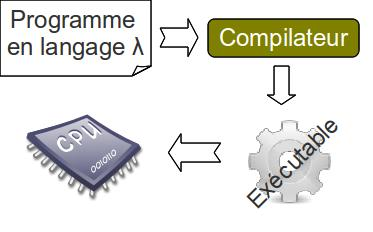
\includegraphics[width=9cm]{images/java-jvm-compil}
\caption{Langage compilé}
\label{compilé}
\end{center}
\end{figure}

%\pagebreak[4]
\index{interprètation}
\marginicon{definition}
\textbf{Définition}

Un langage est \textbf{interprèté} (voir fig. \ref{interprété}) si le code
source est traduit instruction par instruction. Aucun nouveau fichier n'est créé
et les instructions sont traduites à chaque exécution du programme. 

Ces langages nécessitent un \textbf{interprèteur}\footnote{Certaines personnes 
préfèrent parler d'un interprète mais le terme prête à confusion.}.

\begin{figure}[h]
\begin{center}
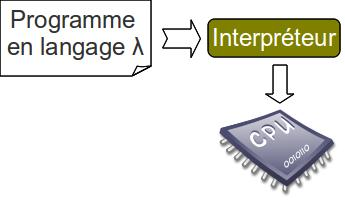
\includegraphics[width=7cm]{images/java-jvm-interp}
\caption{Langage interprété}
\label{interprété}
\end{center}
\end{figure}

Les deux approches ont leurs avantages et leurs inconvénients. 

\begin{itemize}
	
	\item Dès lors qu'une machine possède l'interprèteur, le développeur peut
		diffuser son code et le code pourra être exécuté sur la machine\ldots
		quel que soit son OS (\textit{operating system}, système d'exploitation). 

		Le programme fonctionnera sans modification supplémentaire sur une 
		machine MS Windows, Linux ou Mac OS. 

	\item Avec une approche «~interprétée~», pour diffuser un programme, il faut 
		diffuser le code source. S'il s'agit d'un langage compilé, il est possible
		de ne distribuer que le binaire / exécutable.

		Par contre, il existe des «~\textit{décompilateurs}~» qui peuvent
		reconstruire le code source à partir du binaire / exécutable.

	\item La phase de compilation permet de détecter beaucoup de (petites)
		erreurs avant d'exécuter le programme.

	\item L'exécution du binaire / exécutable est plus rapide que
		l'interprétation du code source. 

\end{itemize}

\marginicon{definition}
Java a une approche mixte, il est compilé et ensuite interprèté. Le code source
est compilé et produit un \textit{bytecode} sauvegardé dans un nouveau fichier.
Le \textit{bytecode} est ensuite interprété par une machine virtuelle, la
\textit{jvm} \index{jvm} (\textit{Java Virtual Machine}). 

\bigskip
\begin{figure}[h]
\begin{center}
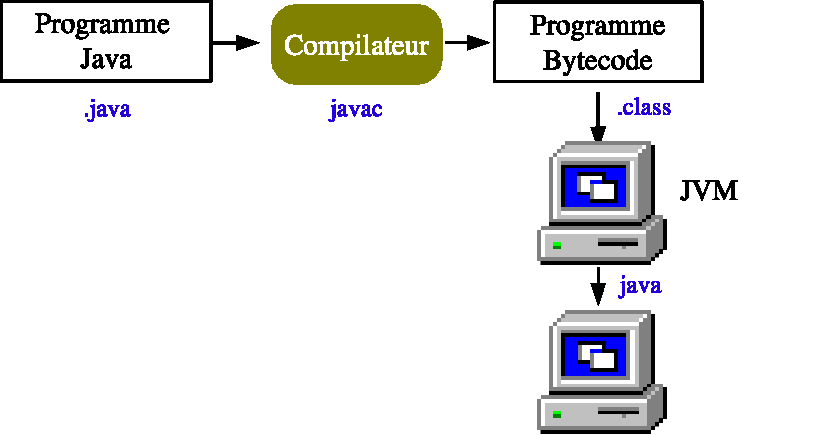
\includegraphics[width=14cm]{images/java-jvm-jvm2}

\caption{Java est compilé et ensuite interprété}
\label{jvm}
\end{center}
\end{figure}

Le \textbf{code source} du programme est écrit dans un fichier texte dont
l'extension sera \texttt{.java}. C'est le fichier que manipule le développeur.
Le code source est la suite l'instructions java. 

À l'aide du \textbf{compilateur} — le programme \texttt{javac} — le fichier est
compilé. Un nouveau fichier ayant comme extension \texttt{.class}, est créé
contenant le \textit{bytecode}.  Ce fichier est destiné à la machine virtuelle.
Voici l'instruction pour compiler le programme.

\begin{term}
	javac MyProgram.java
\end{term}

C'est la machine virtuelle — le programme \texttt{java} — qui est l'interprèteur 
du bytecode. C'est ce programme qui permet d'exécuter le… programme. 

\begin{term}
	java MyProgram
\end{term}

\paragraph{Remarques} Notez que \texttt{javac} prend le nom d'un fichier en
paramètre (avec son extension) alors que \texttt{java} prend le nom d'un
programme — nous dirons une classe bientôt — en paramètre (sans extension donc). 

 


%
%
%
%
\section{Environnement de développement}

\index{environnement}
L'environnement de développement représente l'ensemble des outils nécessaires au
développement, à l'écriture des programmes. 

\subsection{La base}

Il est évidemment nécessaire d'avoir un \textbf{ordinateur} et de le connaitre 
un tant soit peu. Voici quelques compétences nécessaires~:

\begin{itemize}
	\item manipuler des fichiers~: les déplacer, les trouver, les renommer…
	\item ouvrir un terminal;
	\item connaitre son clavier et particulièrement où se trouvent les caractères
		spéciaux. Par exemple~: \verb|{}[];<>"'|;

\end{itemize}

Par contre, que l'OS utilisé soit MS Windows, linux ou Mac OS importe peu pour 
l'apprentissage de l'algorithmique et du développement en Java. 

\subsection{Écrire le code}

\index{ide}
Pour \textbf{écrire le code}, deux approches sont possibles~: l'utilisation 
d'un éditeur de code ou d'un IDE (EDI, Environnement de Développement Intégré).

\begin{enumerate}
	\item \textbf{éditeur de code}

		Un éditeur de code est un éditeur de texte — à ne pas confondre avec un
		traitement de texte — augmenté c'est-à-dire offrant des fonctionnalités
		supplémentaires. Citons par exemple~:

		\begin{itemize}

			\item la coloration syntaxique. Le programme reconnait les mots clés
				du langage, les structures et les écrit en couleur pour
				accroitre la lisibilité du code;

			\item l'indentation automatique et la réindentation du code;

			\item une certaine autocomplétion pour les mots connus du langage 
				et les variables.

		\end{itemize}

		Exemples d'éditeurs de code toutes plateformes, licences et prix
		confondus~: {\itshape (g)Vim, Notepad++, Atom, SublimeText…}
	
		Exemples d'éditeurs de texte inutile pour le développement~: {\itshape
		nano, Notepad, Mousepad}.


	\item \textbf{IDE}

		Un environnement de développement intégré est un programme servant à 
		écrire les programmes. En plus d'un éditeur de code, un IDE compile 
		en arrière plan, a un débogueur, organise les fichiers, crée des fichiers
		(en partie) pré-complétés sur base de \textit{templates}…

		Exemples d'IDE~: {\itshape Netbeans, Eclipse… }

\end{enumerate}

Connaitre et utiliser correctement un éditeur de code et un IDE sont deux
compétences essentielles d'un bon développeur.

\subsection{Exécuter le programme}

Quand le code est écrit, il faut le compiler puis l'exécuter. Les deux
programmes, \texttt{javac} et \texttt{java}, font partie d'un ensemble de
programmes fournis avec le langage Java. Cet ensemble de programmes nécessaires
au développement en Java s'appelle \textbf{JDK}~:\textit{Java Development Kit}
\index{JDK}

Il en existe deux~:

\begin{enumerate}
	
	\item Java est — actuellement — la propriété d'Oracle et c'est Oracle qui
		fournit le JDK officiel. 

		\href{http://www.oracle.com/technetwork/java/javase/downloads}
		{Télécharger Java chez Oracle}

	\item OpenJDK est une alternative libre au JDK officiel Java.

		\href{http://openjdk.java.net/}{Télécharger OpenJDK}

\end{enumerate}


\paragraph {Remarque} Il ne faut pas confondre JDK et JRE\index{JRE}. Un JRE
pour \textit{Java Runtime Environment}, est l'ensemble de programmes — il y en
a moins — nécessaires à l'\textbf{exécution} de programmes Java. Dans ces
programmes se trouve une machine virtuelle java (\textit{JVM}) pour
l'interprètation des programmes java. 

Vous avez probablement déjà un — voire plusieurs — JRE sur votre machine. 


\subsection{Hello world}

Une fois les armes fourbies, il est temps d'écrire son premier programme. Et,
selon la tradition, nous allons écrire un programme qui affiche \textit{Hello
world}.

Un programme Java s'écrit dans une \textbf{classe}. Cette classe porte un nom et
ce nom doit être le même que celui du fichier qui la contient. Nous allons
appeler notre première classe \texttt{Hello}. 

Grâce à mon éditeur de code, je crée le fichier \texttt{Hello.java}
\footnote{%
	Si vous êtes un utilisateur MS Windows, désactivez la propriété
	«\textit{Hide extension for know files types}». Si vous ne le faites pas,
	vous allez — probablement — voir \texttt{Hello.java} alors que le fichier
	que vous créez est \texttt{Hello.java.txt}.
}qui contient~:

\begin{java}
public class Hello{
	public static void main (String[] args) { 
		System.out.println("Hello word");
	}
}
\end{java}

Je compile ma classe~:

\begin{term}
	javac Hello.java
\end{term}

Un fichier \texttt{Hello.class} apparait dans mon répertoire courant. C'est le 
\textit{bytecode} de ma classe. J'exécute ma classe~:

\begin{term}
	java Hello
\end{term}

… et je vois apparaitre dans mon terminal les mots \textbf{Hello world}. 





\section{La grammaire du langage}

Un langage de programmation, dès lors qu'il est compilé et exécuté par une
machine, répond à des règles très strictes. En tout cas, ces règles doivent être
non ambigües. 

Cet ensemble de règles est appelé la \textbf{grammaire du
langage}\index{grammaire} et se trouve dans \textit{The Java Language
Specification}, un ouvrage reprenant toute la spécification du langage Java.
Nous allons y faire référence régulièrement dans ces notes. 

\index{jls}\textbf{JLS} 
\href{https://docs.oracle.com/javase/specs/}
{Télécharger \textit{The Java Language Specification}}

Les \textbf{symboles terminaux} de la grammaire, ceux que l'on peut retrouver en
l'état dans le code sont écrit en police à chasse fixe \texttt{comme ça}. Les
\textbf{règles de production}, qui sont définies ailleurs dans la grammaire, sont
écrites en italiques \textit{comme ça}. 

Dans ces notes, nous utiliserons une \textbf{grammaire simplifiée} par soucis de
simplification pour une première approche du développement sans jamais le
préciser. Celles et ceux qui veulent aller plus loin sont invités  à faire
référence à JLS pour la grammaire complète.

Nous avons dit que le type entier en Java était \pc{int} et que les nombres
réels étaient déclarés grâce au mot clé \pc{double}. Si nous avions voulu
utiliser la grammaire (simplifiée) nous aurions pu écrire~:

\begin{grammaire}
	\grammarrule{NumericType:}
	    \grammarrule{IntegralType}
	    \grammarrule{FloatingPointType}
	
	\grammarrule{IntegralType:}
	    int
	
	\grammarrule{FloatingPointType:}
	    double
\end{grammaire}

Ce qui signifie qu'il existe deux sortes de types numériques~: les nombres
entiers et les nombres à virgule flottante. Pour les nombres entiers, il s'agit
du type \pc{int}. C'est un symbole terminal qui peut se retrouver tel quel dans
un code. Pour les nombres réels — nous avions dit \textit{pseudo-réels} — ou «~à
virgule flottante~», il s'agit du type \pc{double}.

Nous sommes incomplets à ce stade. Les personnes curieuses peuvent aller voir la grammaire complète de ces règles dans \href{https://docs.oracle.com/javase/specs/jls/se10/jls10.pdf}{JLS10} p. 42.


		%===========================================
\chapter{Une question de choix}
%===========================================

	Les \textbf{alternatives}\index{alternatives} permettent de n’exécuter des
	instructions que si une certaine \emph{condition} est vérifiée.  
	Par exemple, si le filtre à café est vide, le remplir. Dans la vie, nous 
	testons notre environnement, dans nos algorithmes
	et dans nos programmes, nous allons tester les données.
	
	Les algorithmes et les programmes vus jusqu’à présent ne proposent qu’un
	seul \og{}chemin\fg{}, une seule \og{}histoire\fg{}.  À chaque exécution de
	l’algorithme, les mêmes instructions s’exécutent dans le même ordres.  Les
	alternatives permettent de créer des histoires différentes, d’adapter les
	instructions aux valeurs concrètes des données.  

	\minitoc 

%===========================================
\section{Le si (\textit{if-then})}
\index{si}\index{if}
%===========================================
		
	Il existe des situations où des instructions ne doivent pas toujours être
	exécutées et un test va nous permettre de le savoir.
	
	\begin{langagenaturel}
		si une certaine condition est vraie alors\\
		\tab exécuter une ou plusieurs actions\\
		fin si\\
		continuer l'algorithme
	\end{langagenaturel}

	Dans la grammaire du langage Java, cette instruction s'écrit~:
	
	\begin{grammaire}
		\grammarrule{IfThenStatement:}
		    if ( \grammarrule{Expression} )
 		        \grammarrule{Statement}
	\end{grammaire}

	\begin{enumerate}
		\item \grammarrule{Expression} représente une expression booléenne. 
			c'est-à-dire ayant comme valeur \pc{true} ou \pc{false}.
		\item \grammarrule{Statement} représente une instruction ou un 
			\textbf{bloc} d'instructions. En langage Java, un bloc 
			\index{bloc} d'instructions est toujours délimités par une paire 
			d'accolades. 
	\end{enumerate}

	\marginicon{attention}
	\textbf{Remarque}

	Attention, un \og{}si\fg{} n’est pas une règle que l’ordinateur doit
	apprendre et exécuter à chaque fois que l’occasion se présente.  La
	condition n’est testée que lorsqu’on arrive à cet endroit de l’algorithme.
	
	\textbf{Exemple}

	Supposons que la variable \pc{nb} contienne un nombre positif ou négatif.
	Et supposons que l’on veuille le rendre positif. Il faudra tester son signe
	et, s’il est négatif, l'inverster.  Par contre, s’il est positif, il n’y
	a rien à faire.  
	
	Voici comment écrire un algorithme sous différentes formes~:
		
	\begin{langagenaturel}
		si nb < 0 alors\\
			\tab nb = -nb\\
		fin si
	\end{langagenaturel}
	
	ou
	
	\begin{langagenaturel}
		if (nb < 0)\\
			\tab nb = -nb\\
	\end{langagenaturel}
	
	Un organigramme aurait cette forme~:

	\begin{center}
		\begin{tikzpicture}[node distance = 2cm, auto]
			\node (start) [startstop] {Start};
			\node (dec1) [decision, below of=start, yshift=-1cm] {nb < 0};
			\draw [arrow] (start) -- (dec1);
			\node (proc1) [process, below of=dec1, yshift=-2cm] {nb = -nb};
			\node (stop) [startstop, below of=proc1] {End};
			\draw [arrow] (dec1) -- node[anchor=south, xshift=-5mm] {true} (proc1);
			\draw [arrow] (dec1) .. controls (4.5,-6) 
				.. node[anchor=east] {false} (stop);
			\draw [arrow] (proc1) -- (stop);
		\end{tikzpicture}	
	\end{center}
	
	En langage Java, le \emph{si} s'écrit comme suit~:

	\begin{java}
if (nb < 0)
	nb = -nb;
	\end{java}

	Pour s'éviter des erreurs, nous utiliserons toujours le bloc d'instructions.
	Nous conseillons de faire de même et nous écrirons~:

	\begin{java}
if (nb < 0){
	nb = -nb;
}
	\end{java}


	Traçons l'algorithme dans deux cas différents pour bien illustrer 
	son déroulement.
	
	\begin{center}
	\begin{tabular}{|>{\centering\arraybackslash}m{1cm}
					|*{2}{>{\centering\arraybackslash}m{1cm}}|}
		\hline
		\rowcolor{black!40}
			\verb_#_  & nb & test \\			
		\hline
			  & -3                   & {}   \\
			1 & {\color{gray}$\mid$} & vrai \\
			2 & 3                    & {}   \\
		\hline
	\end{tabular}
	\qquad
	\begin{tabular}{|>{\centering\arraybackslash}m{1cm}
					|*{2}{>{\centering\arraybackslash}m{1cm}}|}
		\hline
		\rowcolor{black!40}
			\verb_#_  & nb & test \\			
		\hline
			  & 3                    & {}   \\
			1 & {\color{gray}$\mid$} & faux \\
		\hline
	\end{tabular}
	\end{center}
	
	\begin{Emphase}
		\paragraph{Exercice de compréhension}
		Tracez  l'algorithme écrit en langage Java avec les valeurs fournies 
		et donnez la valeur de retour.
		
		\begin{java}
public static int exercice(int a, int b){
	int c;
	c = 2 * a;
	if (c > b){
		c = c-b;
	}
	return c;
}
		\end{java}
		
		\begin{multicols}{2}
		\begin{itemize}
		\item \pc{exercice(2, 5)} = \_\_\_
		\item \pc{exercice(4, 1)} = \_\_\_
		\end{itemize}
		\end{multicols}	
	\end{Emphase}


	\pagebreak[4]
%===============================
\section{Le si-sinon (\textit{if-then-else})}
\index{if-else}\index{si-sinon}
%===============================
	
	La construction \pc{si-sinon} permet d’exécuter certaines instructions ou
	d’autres en fonction d’un test.  
	
	\begin{langagenaturel}
		si une certaine condition est vraie alors\\
			\tab exécuter une ou plusieurs actions\\
		sinon (la condition est alors fausse)\\
			\tab exécuter d'autres actions\\
		fin si\\
		continuer l'algorithme 
	\end{langagenaturel}

	Dans la grammaire du langage Java, cette instruction s'écrit~:

	\begin{grammaire}
		\grammarrule{IfThenElseStatement:}
		    if ( \grammarrule{Expression} )
		        \grammarrule{Statement}
		    else
		        \grammarrule{Statement}
	\end{grammaire}

	\textbf{Exemple}

	Pour illustrer cette instruction, nous allons écrire un algorithme qui 
	recherche le maximum de deux nombres. 
	
	Pour déterminer le maximum de deux nombres, c’est-à-dire la plus grande
	des deux valeurs, il y aura deux chemins possibles.  Le maximum devra
	prendre la valeur du premier nombre ou du second selon que le premier est
	plus grand que le second ou pas.

	Voici comment écrire cet algorithme sous différentes formes~:

	\begin{langagenaturel}
		if (nb1 > nb2)\\
			\tab max = nb1\\
		else\\
			\tab max = nb2\\
	\end{langagenaturel}

	Un organigramme aurait cette forme~:
	
	\begin{center}
		\begin{tikzpicture}[node distance = 2cm, auto]
			\node (start) [startstop] {Start};
			\node (dec1) [decision, below of=start, yshift=-1cm] {nb1 > nb2};
			\draw [arrow] (start) -- (dec1);
			\node (proc1) [process, below of=dec1, yshift=-2cm, xshift=-2cm] 
				{max = nb1};
			\node (proc2) [process, below of=dec1, yshift=-2cm, xshift=2cm] 
				{max = nb2};
			\node (stop) [startstop, below of=dec1, yshift=-5cm] {End};
			\draw [arrow] (dec1) -- node[anchor=west, xshift=-10mm] {true} (proc1);
			\draw [arrow] (dec1) -- node[anchor=east, xshift=-1mm] {false} (proc2);
			\draw [arrow] (proc1) -- (stop);
			\draw [arrow] (proc2) -- (stop);
		\end{tikzpicture}	
	\end{center}
	
	En supposant les variables déclarées, le \textit{si-alors}, s'écrit comme
	suit en langage Java~:

	\begin{java}
if (nb1 > nb2){		
	max = nb1;
} else {
	max = nb2;
}
	\end{java}

	Traçons l'algorithme dans différentes situations.
	
	\begin{center}
	\begin{tabular}{|>{\centering\arraybackslash}m{6mm}
					|*{4}{>{\centering\arraybackslash}m{1cm}}|}
		\hline
		\rowcolor{gray!40}
			\verb_#_  & nb1 & nb2 & max & test \\			
		\hline
			  & 3 & 2 & indéfini & {} \\
			1 & {\color{gray}$\mid$} & {\color{gray}$\mid$} & indéfini & vrai \\
			2 & {\color{gray}$\mid$} & {\color{gray}$\mid$} & 3        & {} \\
		\hline
	\end{tabular}
	\end{center}

	\begin{center}
	\begin{tabular}{|>{\centering\arraybackslash}m{6mm}
					|*{4}{>{\centering\arraybackslash}m{1cm}}|}
		\hline
		\rowcolor{gray!40}
			\verb_#_  & nb1 & nb2 & max & test \\			
		\hline
			  & 4 & 42 & indéfini & {} \\
			1 & {\color{gray}$\mid$} & {\color{gray}$\mid$} & indéfini & faux \\
			4 & {\color{gray}$\mid$} & {\color{gray}$\mid$} & 42        & {} \\
		\hline
	\end{tabular}
	\end{center}
	
	Le cas où les deux nombres sont égaux est également géré.
	
	\begin{center}
	\begin{tabular}{|>{\centering\arraybackslash}m{1cm}
					|*{4}{>{\centering\arraybackslash}m{1cm}}|}
		\hline
		\rowcolor{gray!40}
			\verb_#_  & nb1 & nb2 & max & test \\			
		\hline
			  & 4 & 4 & indéfini & {} \\
			1 & {\color{gray}$\mid$} & {\color{gray}$\mid$} & indéfini & faux \\
			4 & {\color{gray}$\mid$} & {\color{gray}$\mid$} & 4        & {} \\
		\hline
	\end{tabular}
	\end{center}
	
	\begin{Emphase}
		\paragraph{Exercice de compréhension}

		Tracez ces algorithmes ou programmes avec les valeurs fournies et donnez
		la valeur de retour.
	

		\begin{java}
public static int exercice(int a, int b){
	int c;
	if (a > b){
		c = a/b;
	} else {
		c = b%a;
	}
}
		\end{java}
	
		\begin{multicols}{2}
		\begin{itemize}
		\item \pc{exercice(2, 3)} = \_\_\_
		\item \pc{exercice(4, 1)} = \_\_\_
		\end{itemize}
		\end{multicols}
	

		\begin{java}
public static int exercice(int x1, int x2){
	boolean ok;
	ok = x1 > x2;
	if (ok){
		ok = ok && x1 == 4;
	} else {
		ok = ok || x2 == 3;
	}
	return x1 + x2;
}
		\end{java}
		
		\medskip
		\begin{multicols}{2}
		\begin{itemize}
		\item \pc{exercice(2, 3)} = \_\_\_
		\item \pc{exercice(4, 1)} = \_\_\_	
		\end{itemize}
		\end{multicols}	
		
	\end{Emphase}	
	
	\clearpage

%============================
\section{Le si-sinon-si}
\index{si-sinon-si}
%============================

	Avec cette construction, il est possible d'indiquer à un endroit de
	l’algorithme plus de deux chemins possibles et dès lors que la première
	condition est fausse, tester une condition supplémentaire à chaque étape. 
	
	\begin{langagenaturel}
		si une certaine condition est vraie alors\\
			\tab exécuter une ou plusieurs actions\\
		sinon si une autre condition est vraie alors\\
			\tab exécuter d'autres actions\\
		sinon \\
			\tab exécuter encore d'autres actions\\
		fin si\\
		continuer l'algorithme
	\end{langagenaturel}

	Dans la grammaire du langage Java, il n'y a pas d'instruction
	supplémentaire. Un \textit{si-sinon-si} n'étant que des \textit{si-sinon}
	imbriqués un peu comme suit~:

	\begin{grammaire}
	    if ( \grammarrule{Expression} )
	        \grammarrule{Statement}
	    else
	        if ( \grammarrule{Expression} )
	            \grammarrule{Statement}
	        else
	            \grammarrule{Statement}
	\end{grammaire}
	
	…qui seront généralement indentés comme suit~:
	
	\begin{grammaire}
	    if ( \grammarrule{Expression} )
	        \grammarrule{Statement}
	    else if ( \grammarrule{Expression} )
	        \grammarrule{Statement}
	    else
	       	\grammarrule{Statement}
	\end{grammaire}
	
	… mais voyons cela sur un exmeple. 

	\textbf{Exemple}
	
	Supposons que l'on veuille mettre dans la chaine \pc{signe} la valeur
	\pc{"positif"}, \pc{"négatif"} ou \pc{"nul"} selon qu’un nombre donné est
	positif, négatif ou nul.

	Voici comment écrire cet algorithme sous différents formats~:

	\begin{langagenaturel}
		if (nb > 0)\\
			\tab signe = "positif"\\
		else if (nb == 0)\\
			\tab signe = "nul"\\
		else\\
			\tab signe = "négatif"
	\end{langagenaturel}

	Un organigramme aurait cette allure~:
	
	\begin{center}
		\begin{tikzpicture}[node distance = 2cm, auto]
			\node (start) [startstop] {Start};
			\node (dec1) [decision, below of=start, yshift=-.5cm, 
				text width=.5cm] {};
			\draw [arrow] (start) -- (dec1);
			\node (proc1) [process, below of=dec1, yshift=-2cm, xshift=-4cm] 
				{s = "positif"};
			\node (proc2) [process, below of=dec1, yshift=-2cm] 
				{s = "nul"};
			\node (proc3) [process, below of=dec1, yshift=-2cm, xshift=4cm] 
				{s = "négatif"};
			\node (stop) [startstop, below of=dec1, yshift=-5cm] {End};
			\draw [arrow] (dec1) -- 
				node[anchor=west, xshift=-17mm] {nb>0} (proc1);
			\draw [arrow] (dec1) -- 
				node[anchor=east, xshift=-1mm] {nb == 0} (proc2);
			\draw [arrow] (dec1) -- 
				node[anchor=east, xshift=-1mm] {nb<0} (proc3);
			\draw [arrow] (proc1) -- (stop);
			\draw [arrow] (proc2) -- (stop);
			\draw [arrow] (proc3) -- (stop);
		\end{tikzpicture}	
	\end{center}
	
	Comme dit plus haut, en langage Java, il n'y a pas de structure particulière
	pour ce test. Le \pc{if-then-else} fait bien l'affaire. Seule l'indentation
	change un peu pour plus de lisibilité. Ce test peut donc s'écrire — en
	supposant toujours que les variables sont déclarées — comme ceci~:

	\begin{java}
if (nb > 0){
	s = "positif";
} else if (nb == 0) {
	s = "nul";
} else {
	s = "négatif";
}
	\end{java}

	Traçons l'algorithme dans différentes situations. 
	
	\begin{center}
	\begin{tabular}{|*{2}{>{\centering\arraybackslash}m{4mm}}
					 *{2}{>{\centering\arraybackslash}m{9mm}}|}
		\hline
		\rowcolor{black!40}
			\verb_#_  & nb & signe & test \\			
		\hline
			  & 2                    & indéfini             & {}   \\
			1 & {\color{gray}$\mid$} & {\color{gray}$\mid$} & vrai \\
			2 & {\color{gray}$\mid$} & "positif"            & {}   \\
		\hline
	\end{tabular}
	\end{center}
	
	\begin{center}
	\begin{tabular}{|*{2}{>{\centering\arraybackslash}m{4mm}}
					 *{2}{>{\centering\arraybackslash}m{9mm}}|}
		\hline
		\rowcolor{black!40}
			\verb_#_  & nb & signe & test \\			
		\hline
			  & 0                    & indéfini             & {}   \\
			1 & {\color{gray}$\mid$} & {\color{gray}$\mid$} & faux \\
			3 & {\color{gray}$\mid$} & {\color{gray}$\mid$} & vrai \\
			4 & {\color{gray}$\mid$} & "nul"                & {}   \\
		\hline
	\end{tabular}
	\quad
	\begin{tabular}{|*{2}{>{\centering\arraybackslash}m{4mm}}
					 *{2}{>{\centering\arraybackslash}m{9mm}}|}
		\hline
		\rowcolor{black!40}
			\verb_#_  & nb & signe & test \\			
		\hline
			  & -5                   & indéfini             & {}   \\
			1 & {\color{gray}$\mid$} & {\color{gray}$\mid$} & faux \\
			3 & {\color{gray}$\mid$} & {\color{gray}$\mid$} & faux \\
			6 & {\color{gray}$\mid$} & "négatif"            & {}   \\
		\hline
	\end{tabular}
	\end{center}
	

	\paragraph{Remarques.}
	\begin{itemize}
	\item
		Pour le dernier cas, on se contente
		d’un \pc{\K{sinon}} sans indiquer la condition~;
		ce serait inutile, elle serait toujours vraie.
	\item
		Le \pc{\K{si}} et le \pc{\K{si-sinon}} 
		peuvent être vus comme des cas particuliers du 
		\pc{\K{si-sinon-si}}.
	\item
		On pourrait écrire la même chose 
		avec des \pc{\K{si-sinon}} imbriqués
		mais le \pc{\K{si-sinon-si}} est plus lisible.
	\item Lorsqu’une condition est testée, on sait que toutes celles au-dessus se
		sont avérées fausses.  Cela permet parfois de simplifier la condition.

		\textbf{Exemple.}
		Supposons que le prix unitaire d’un produit (\pc{prixUnitaire})
		dépende de la quantité achetée (\pc{quantité}). 
		En dessous de 10 unités, on le paie 10\texteuro{} l’unité.
		De 10 à 99 unités, on le paie 8\texteuro{} l’unité.
		À partir de 100 unités, on paie 6\texteuro{} l’unité.

		\begin{java}
if (quantité < 10){
	prixUnitaire = 10;
} else if (quantité < 100) {
	// On sait que la quantité est plus grande
	// ou égale à 10. Inutile de tester. 
	prixUnitaire = 8;
} else {
	prixUnitaire = 6;
}
		\end{java}
		
	\end{itemize}


%==========================================
\section{Expression booléenne}
\index{expression booléenne}
\label{expression booléenne}
%==========================================

Nous avons dit que dans un test, l'\textit{expression} était une expression
booléenne et nous avons vu quelques opérateurs intervenant dans ces
expressions.  Revenons plus en détail sur ce concept. 

\marginicon{definition}
\textbf{Definition.} Une expression booléenne est une expression — c'est-à-dire
le résultat d'un calcul — dont la valeur est booléenne~: \pc{true} ou
\pc{false}. 

Une telle expression se compose grâce~: 

\begin{enumerate}
	\index{opérateurs relationnels}
	\item aux opérateurs relationnels (\textit{relational operator} ou 
		\textit{comparators}\index{comparators});
		
		Un opérateur relationnel est un opérateur dont la valeur
		est booléenne et les opérandes numériques. 

		\begin{grammaire}
			\grammarrule{RelationalOperator:}
			    \grammarrule{(one of)}
			    < > <= >=
		\end{grammaire}
		
	\index{opérateurs d'égalité}
	\item aux opérateurs d'égalité (\textit{equality operators});

		Un opérateur d'égalité est un opérateur dont la valeur
		est booléenne et les opérandes de même type (à conversion près). 

		\begin{grammaire}
			\grammarrule{EqualityOperator:}
			    \grammarrule{(one of)}
			    == != 
		\end{grammaire}

	\index{opérateurs logiques}
	\item au complément logique (\textit{logical complement operator}) et 
		aux opérateurs conditionnels 
		(\textit{conditionals operators}\index{conditionals operators});

		Le complément logique et les opérateurs conditionnels sont des
		opérateurs dont la valeur est booléenne et le ou les opérandes également
		booléens. 

		Le \pc{\&\&} est prioritaire sur le \pc{||}.

		\begin{grammaire}
			\grammarrule{LogicalComplementOperator:}
			    !
			\grammarrule{ConditionalOperator:}
			    \grammarrule{(one of)}
			     || &&
		\end{grammaire}
\end{enumerate}



%==========================================
\section{Le selon-que (\textit{switch})}
\index{selon-que}\index{switch}
%==========================================

	Cette nouvelle instruction permet d’écrire plus lisiblement \emph{certains}
	\pc{\K{si-sinon-si}}, plus précisément quand le choix d’une branche dépend
	de la valeur précise d’une variable (ou d’une expression).

	\begin{langagenaturel}
		selon que la variable vale~:\\
			\tab — une valeur~:\\
				\tab\tab exécuter une ou plusieurs actions\\
			\tab — une autre valeur~:\\
				\tab\tab exécuter d'autres actions\\
			\tab — encore une autre valeur~:\\
				\tab\tab exécuter d'autres actions\\
			\tab — et une dernière valeur~:\\
				\tab\tab exécuter d'autres actions\\
		fin selon que 
	\end{langagenaturel}

	Dans la grammaire  du langage Java, cette instruction, \textit{switch}, 
	s'écrit (grammaire simplifiée)~:

	\begin{grammaire}
		\grammarrule{SwitchStatement:}
		    switch ( \grammarrule{Expression} ) \grammarrule{SwitchBlock}

		\grammarrule{SwitchBlock:}
		    \grammarrule{SwitchLabels Statement}

		\grammarrule{SwitchLabel:}
		    case \grammarrule{ConstantExpression}:
		    default:
	\end{grammaire}
	
	\begin{itemize}
		\item l'expression ne peut pas être de n'importe quel type. À ce stade, 
			elle peut être, un entier ou une chaine et nous rencontrerons 
			d'autres types plus tard~;
		\item \textit{Statement} peut être une instuction ou plusieurs~;
		\item \textit{SwitchLabels} (avec un \textit{s}) ce sont plusieurs 
			«~\texttt{case}~»~;
		\item le \textit{switch} en java peut être vu comme un «~\textit{saut}
			au bon label~». Dès lors que l'instruction a trouvé le bon
			\textit{case}, l'éxécution des instructions continue. Il faut
			explicitement demander de sortir du \textit{switch} en utilisant
			l'instruction \textbf{\pc{break}}\index{break}~.
	\end{itemize}

	… mais voyons ça sur un exemple. 	

	\textbf{Exemple.}
	
	Imaginons qu’une variable (\pc{dayNumber}) contienne un numéro de jour de la
	semaine et qu’on veuille mettre dans une variable (\pc{dayName}) le nom du
	jour correspondant ("lundi" pour 1, "mardi" pour 2\dots)
	
	Une solution avec un \pc{\K{si-sinon-si}} est possible 
	mais le \pc{\K{selon-que}} (\textit{switch}) est plus lisible dans ce cas.

	Voyons comment écrire un algorithme sous différentes formes~:

	\begin{langagenaturel}
		switch ( dayNumber )\\
			\tab — 1~:\\
				\tab\tab dayName = "lundi"\\
			\tab — 2~:\\
				\tab\tab dayName = "mardi"\\
			\tab — 3~:\\
				\tab\tab dayName = "mercredi"\\
			\tab — 4~:\\
				\tab\tab dayName = "jeudi"\\
			\tab — 5~:\\
				\tab\tab dayName = "vendredi"\\
			\tab — 6~:\\
				\tab\tab dayName = "samedi"\\
			\tab — 7~:\\
				\tab\tab dayName = "dimanche"
	\end{langagenaturel}

	En langage Java~:

	\begin{java}
switch (dayNumber) {
	case 1: 
		dayName = "lundi"; 
		break;
	case 2: 
		dayName = "mardi"; 
		break;
	case 3: 
		dayName = "mercredi"; 
		break;
	case 4: 
		dayName = "jeudi"; 
		break;
	case 5: 
		dayName = "vendredi"; 
		break;
	case 6: 
		dayName = "samedi"; 
		break;
	case 7: 
		dayName = "dimanche";
}
	\end{java}
		
	\paragraph{Remarques.}
	\begin{itemize}
	\item
		Il peut y avoir plusieurs valeurs pour un cas donné.
	\item
		Il peut y avoir un cas par défaut, \pc{default}
		qui sera exécuté si la valeur n’est pas reprise par ailleurs.
	\end{itemize}
	
	
	

		%===========================================
%\chapter{Décomposer le problème}
\chapter{Module et références}
\index{décomposer le code}
\index{primitif}\index{reference}
%===========================================

\minitoc

%===================
\section{Décomposer le problème}
%===================

	Jusqu’à présent, les problèmes que nous avons abordés étaient relativement
	petits.  Nous avons pu les résoudre avec un algorithme d’un seul tenant.
	
	Dans la réalité, les problèmes sont plus conséquents et il devient
	nécessaire de les décomposer en sous-problèmes.  On parle d’une
	\emph{approche modulaire}.  Les avantages d’une telle décomposition sont
	multiples.
	
	\begin{itemize}
	\item
		\textbf{Cela permet de libérer l’esprit.}
		L’esprit humain ne peut pas traiter trop d’informations à la fois
		(\emph{surcharge cognitive}).
		Lorsqu’un sous-problème est résolu,
		il peut se libérer l’esprit et attaquer un autre sous-problème.
	\item
		\textbf{On peut réutiliser ce qui a été fait.}
		Si un même sous-problème apparait plusieurs fois
		dans un problème ou à travers plusieurs problèmes,
		il est plus efficace de le résoudre une fois et
		de réutiliser la solution.
	\item
		\textbf{On accroit la lisibilité.} Si,  un algorithme, appelle un autre
		algorithme pour résoudre un sous-problème, le lecteur ou la lectrice
		verra un nom d’algorithme qui peut être plus parlant que les
		instructions qui se cachent derrière, même s’il y en a peu.  Par
		exemple, \pc{dizaine(nb)} est plus parlant que \pc{nb MOD 100 DIV 10}
		pour calculer le nombre de dizaines d’un nombre.
	
\end{itemize}

	Parmis les autres avantages, que vous pourrez moins percevoir en début
	d’apprentissage, citons la possibilité de répartir le travail dans une
	équipe.
	
	Un algorithme qui résout une partie de problème
	est parfois appelé \textbf{fonction}\index{fonction}, 
	\textbf{procédure}\index{procédure}, 
	\textbf{méthode}\index{méthode} ou encore
	\textbf{module}\index{module}
	en fonction du langage et du contexte.
	Il y a quelques nuances mais elles importent peu ici.
	
%===================
\section{Exemple}
%===================

	Illustrons l’approche modulaire sur le calcul du maximum de 3 nombres.

	\begin{center}
	\flowalgoddd{a (réel)}{b (réel)}{c (réel)}{max3}{réel}
	\end{center}
	
	Commençons par écrire la solution du problème plus simple~:~
	le maximum de 2 nombres.

	\begin{minipage}{6cm}
		\flowalgodd{a (réel)}{b (réel)}{max2}{réel}
	\end{minipage}
	\quad
	\begin{minipage}{7cm}
		\begin{java}
public static double max2(double a, double b){
	double max;
	if (a > b){
		max = a;
	} else {
		max = b;
	}
	return max;
}
		\end{java}
	\end{minipage}
	
	Pour le maximum de 3 nombres, il existe plusieurs approches.  Voyons
	celle-ci~:

	\begin{enumerate}
		\item  Calculer le maximum des deux premiers nombres, soit \pc{maxab}
		\item  Calculer le maximum de \pc{maxab} et du troisième nombre, ce qui donne le résultat.
	\end{enumerate}

	\clearpage
	Elle s'illustre comme suit~:
	
	\begin{center}
	\begin{tikzpicture}[auto]
		\sffamily
		\node (a) at (0,4) {a (réel)};
		\node (b) at (0,2) {b (réel)};
		\node (c) at (0,0) {c (réel)};
		\node[draw,rounded corners] (max2a) at (2,3) {max2};
		\node[draw,rounded corners] (max2b) at (4,2) {max2};
		\node (r) at (6,2) {réel};
		\draw[rounded corners] (1,0) rectangle (5,4) node[above] {max3};
		\draw[->,thick] (a) to (max2a);
		\draw[->,thick] (b) to (max2a);
		\draw[->,thick] (c) to (max2b);
		\draw[->,thick] (max2a) to (max2b);
		\draw[->,thick] (max2b) to (r);
	\end{tikzpicture}	
	\end{center}
	
	Sur base de cette idée, 
	on voit que calculer le maximum de trois nombres
	peut se faire en calculant deux fois le maximum de deux nombres.
	On ne va évidemment pas \emph{recopier}%
	\footnote{
		Cette approche serait fastidieuse,
		engendrerait de nombreuses erreurs lors du recopiage
		et serait difficile à lire. Même le copier/coller n'est pas une bonne 
		solution. Il diminue la lisibilité et rend la refactorisation et 
		l'évolution des alogorithmes et des programmes plus compliquées.
	} dans notre solution
	ce qu’on a écrit pour le maximum de deux nombres~;
	on va plutôt y faire référence, 
	c’est-à-dire appeler l’algorithme \pc{max2}. 
	Ce qui donne~:

	\begin{java}
public static double max3(double a, double b, double c){
	double maxab, max;
	maxab = max2(a, b);
	max = max2(maxab, c);
	return max;
}
	\end{java}

	qui peut se simplifier en~:
	
	\begin{java}
public static double max3(double a, double b, double c){
	return max2(max2(a, b), c);
}
	\end{java}

%===================
\section{Paramètres et valeur de retour}
\index{paramètres}\label{paramètres}
%=======================

	Jusqu’à présent, nous avons considéré que les paramètres d’un algorithme
	(ou \emph{module}\index{module}) correspondent à ses données et que le
	résultat, unique, est retourné.

	Il s’agit d’une situation fréquente mais pas obligatoire que nous pouvons
	généraliser.  De manière générale nous pouvons concevoir trois sortes de
	paramètres. Nous verrons ensuite ce qu'il en est en langage Java. 

	%==================================
	\subsection{Le paramètre en entrée}
	\label{param.entrée}
	%==================================

		Le paramètre en \textbf{entrée} est ce que nous connaissons déjà.  Il
		correspond à une donnée de l’algorithme.  Une valeur va lui être
		attribuée en début d’algorithme et elle ne sera pas modifiée.  On pourrait
		faire suivre le nom du paramètre d’une flèche vers le bas (\In) pour
		rappeler son rôle mais ce n'est pas obligatoire lorsqu'il n'y a pas
		d'ambiguïté.
		
		Lors de l’appel, c'est une \textbf{valeur} qui est fournie ou, plus
		généralement une expression dont la valeur sera donnée au paramètre.
		Voici un cas général de paramètre en entrée.
		
		\begin{minipage}{4cm}
			\begin{pseudocode}
				\LComment {Code}
				\LComment {appelant}
				\Stmt myAlgo(expr)
				\Empty
			\end{pseudocode}
		\end{minipage}
		\quad
		\begin{minipage}{8cm}
			\begin{pseudocode}
				\LComment {Code appelé}
				\Algo{myAlgo}{\Par{par\In}{integer}}{}
				\Stmt \dots
				\EndAlgo 
			\end{pseudocode}
		\end{minipage}
		
		C’est comme si l’algorithme \pc{myAlgo} commençait par l’affectation
		\pc{par \Gets expr}.
		
		\textbf{Exemple.} 
		Reprenons l’exemple de \pc{max3}
		en ajoutant un petit test.

		\begin{pseudocode}[1]
			\Algo{test}{}{} \RComment {Code appelant}
				\Decl {max}{real}
				\Let max \Gets max3(3, 2, 5)
				\Write max
			\EndAlgo
			\Empty
			\Algo{max3}{\Par{a\In, b\In, c\In}{reals}}{real}
				\RComment {Code appelé}
				\Decl{maxab, max}{reals}
				\Let maxab \Gets max2(a,b)
				\Let max \Gets max2(maxab,c)
				\Return max
			\EndAlgo
		\end{pseudocode}

		Traçons son exécution.
		
		\begin{tabular}{|>{\centering\arraybackslash}m{1.1cm}
						|>{\centering\arraybackslash}m{13mm}
						|*{5}{>{\centering\arraybackslash}m{13mm}}|}
			\hline
			\rowcolor{black!50}
			  & \pc{test} & \multicolumn{5}{c|}{\pc{max3}} \\
			\hline
			\rowcolor{black!30}
			\# & max  & {a} & {b} & {c} & {maxab} & {max}\\
			\hline
			2    & indéfini             &                      &                      &                      &                      &          \\
			3,7  & {\color{gray}$\mid$} & 3                    & 2                    & 5                    &                      &          \\
			8    & {\color{gray}$\mid$} & {\color{gray}$\mid$} & {\color{gray}$\mid$} & {\color{gray}$\mid$} & indéfini             & indéfini \\
			9    & {\color{gray}$\mid$} & {\color{gray}$\mid$} & {\color{gray}$\mid$} & {\color{gray}$\mid$} & 3                    & indéfini \\
			10   & {\color{gray}$\mid$} & {\color{gray}$\mid$} & {\color{gray}$\mid$} & {\color{gray}$\mid$} & {\color{gray}$\mid$} & 5        \\
			11,3 & 5                    &                      &                      &                      &                      &          \\
			\hline
		\end{tabular}
		
		\paragraph{Notez bien~:} Dans cet exemple, on trouve deux fois la
		variable \pc{max}.  Il s’agit bien de deux variables
		\textbf{différentes}~; l’une est définie et connue dans \pc{test}~;
		l’autre l’est dans \pc{max3}.
		
%	%==================================
%	\subsection{Le paramètre en sortie}
%	%==================================
%
%		Le paramètre en \textbf{sortie} correspond à un résultat de
%		l’algorithme.  Avec la notation que nous utilisons, un algorithme ne
%		peut retourner qu’une seule valeur ce qui est parfois une contrainte
%		trop forte.  Les paramètres en sortie vont permettre à l’algorithme de
%		fournir plusieurs réponses.  On fera suivre le nom du paramètre d’une
%		flèche vers le haut (\Out) pour rappeler son rôle.  Un tel paramètre
%		n’aura pas de valeur au début de l’algorithme mais s’en verra attribuer
%		une par l’algorithme.
%		
%		Lors de l’appel, on fournit une \textbf{variable}
%		qui recevra la valeur finale du paramètre.
%		Voici un cas général de paramètre en sortie.
%		
%		\begin{minipage}{4cm}
%			\begin{pc}
%				\LComment {Code appelant}
%				\Stmt myAlgo(variable)
%				\Empty
%			\end{pc}
%		\end{minipage}
%		\quad
%		\begin{minipage}{8cm}
%			\begin{pc}
%				\LComment {Code appelé}
%				\Entete{myAlgo}{\Par{par\Out}{entier}}{}
%				\Stmt \dots
%			\end{pc}
%		\end{minipage}
%
%		Il n’y a \textbf{pas de \pc{\algorithmicreturn}}
%		puisque les résultats sont en paramètres de sortie et pas comme
%		valeur \emph{retournée}.
%		C’est comme si,
%		à la fin de l’algorithme appelé,
%		on avait l’assignation~:
%		\pc{variable \Gets par}.
%		
%		\paragraph{Exemple.}
%		On peut envisager un algorithme
%		qui reçoit une durée exprimée en seconde
%		et fournisse trois paramètres en sortie
%		correspondant à cette même durée exprimée en heures, minutes et secondes.
%		En voici le schéma et la solution~:
%		\begin{center}
%		\flowalgorrr{totalSec (entier)}{versHMS}{heuresÉcoulées (entier)}{minutesÉcoulées (entier)}{secondesÉcoulées (entier)}
%		\end{center}
%			
%		Voici une solution et un appel possible.
%		\begin{pc}[1]
%			\Algo{versHMS}{\Par{totalSec\In, heuresÉcoulées\Out, minutesÉcoulées\Out, secondesÉcoulées\Out}{\\\hfill entiers}}{}
%				\Let heuresÉcoulées \Gets totalSec DIV (60*60)
%				\Let minutesÉcoulées \Gets totalSec MOD (60*60) DIV 60				
%				\Let secondesÉcoulées \Gets totalSec MOD 60
%			\EndAlgo
%			\Empty
%			\Algo{test}{}{}
%				\Decl{heure,minute,seconde}{entiers}
%				\Stmt versHMS(65536, heure, minute, seconde)
%				\Write heure, minute, seconde
%			\EndAlgo
%		\end{pc}
%		
%		Traçons-le.
%
%		\begin{small}
%		\begin{tabular}{|>{\centering\arraybackslash}m{7mm}
%						|*{3}{>{\centering\arraybackslash}m{9mm}}
%						|>{\centering\arraybackslash}m{10mm}
%						 *{3}{>{\centering\arraybackslash}m{19mm}}
%						|}
%			\hline
%			  & \multicolumn{3}{c|}{\pc{test}} & \multicolumn{4}{c|}{\pc{versHMS}} \\
%			\hline
%			\# & {\scriptsize heure} & {\scriptsize minute} & {\scriptsize seconde} & {\scriptsize totalSec} & {\scriptsize heuresEcoulées} & {\scriptsize minutesEcoulées} & {\scriptsize secondesEcoulées}\\
%			\hline
%			9     & indéfini & indéfini & indéfini & {} & {} & {} & {} \\
%			10, 1 & {\color{gray}$\mid$} & {\color{gray}$\mid$} & {\color{gray}$\mid$} & 65536 & indéfini & indéfini & indéfini \\
%			3     & {\color{gray}$\mid$} & {\color{gray}$\mid$} & {\color{gray}$\mid$} & {\color{gray}$\mid$} & 18 & {\color{gray}$\mid$} & {\color{gray}$\mid$} \\
%			4     & {\color{gray}$\mid$} & {\color{gray}$\mid$} & {\color{gray}$\mid$} & {\color{gray}$\mid$} & {\color{gray}$\mid$} & 12 & {\color{gray}$\mid$} \\
%			5     & {\color{gray}$\mid$} & {\color{gray}$\mid$} & {\color{gray}$\mid$} & {\color{gray}$\mid$} & {\color{gray}$\mid$} & {\color{gray}$\mid$} & 16 \\
%			6, 10 & 18 & 12 & 16 &  &  &  &  \\
%			\hline
%		\end{tabular}
%		\end{small}
%				
	%==================================
	\subsection{Le paramètre en entrée-sortie}
	%==================================

		Le paramètre en \textbf{entrée-sortie} est un paramètre tel que:
		\begin{itemize}
			\item l'algorithme reçoit une valeur en entrée;
			\item le paramètre peut être modifié.
		\end{itemize}

		Cela signifie que l’algorithme a pour but de modifier le paramètre.  Un
		tel paramètre parrait être suivi d’une double flèche (\InOut).
	
		C'est une \textbf{une variable} qui doit être passée en paramètre.  Sa
		valeur est donnée au paramètre au début de l’algorithme.  À la fin de
		l’algorithme, la variable reçoit la valeur du paramètre.  Voici un cas
		général de paramètre en sortie.
		
		\begin{minipage}{4cm}
			\begin{pseudocode}
				\LComment {Code}
				\LComment {appelant}
				\Stmt myAlgo(variable)
				\Empty
			\end{pseudocode}
		\end{minipage}
		\quad
		\begin{minipage}{8cm}
			\begin{pseudocode}
				\LComment {Code appelé}
				\Algo{myAlgo}{\Par{par\In\Out}{entier}}{}
				\Stmt \dots
				\EndAlgo 
			\end{pseudocode}
		\end{minipage}

		C’est comme si, dans le code appelé, il y avait une première ligne pour
		donner sa valeur au paramètre (\pc{par \Gets variable}) et une dernière
		ligne pour effectuer l’assignation opposée (\pc{variable \Gets par}). Il
		n’y a pas de \pc{\algorithmicreturn}.
				
		\paragraph{Exemple.}

		Nous avons vu un algorithme qui retourne la valeur absolue d’un nombre.
		Nous pourrions imaginer une variante qui \textbf{modifie} le nombre reçu.
		En voici le schéma et la solution avec un appel possible~:

		\begin{minipage}{.3\linewidth}		
			\begin{center}
			\flowalgov{nb (réel)}{valAbsolue}
			\end{center}
		\end{minipage}
		\quad
		\begin{minipage}{.6\linewidth}		
			\begin{pseudocode}[1]
				\Algo{valAbsolue}{\Par{nb\In\Out}{réel}}{}
					\If{nb<0}
						\Let nb \Gets -nb
					\EndIf
				\EndAlgo
				\Empty
				\Algo{test}{}{}
				\Decl{température}{réel}
				\Let température \Gets -12.5
				\Stmt valAbsolue(température)
				\Write température
				\EndAlgo
			\end{pseudocode}
		\end{minipage}
		
		Traçons-le.
		
		\begin{tabular}{|>{\centering\arraybackslash}m{1cm}
						|>{\centering\arraybackslash}m{20mm}
						|*{2}{>{\centering\arraybackslash}m{20mm}}|}
			\hline
			\rowcolor{black!50}
			  & \pc{test} & \multicolumn{2}{c|}{\pc{valAbsolue}} \\
			\hline
			\rowcolor{black!30}
			\# & température  & nb & test \\
			\hline
			8     & indéfini &  & \\
			9     & -12.5    &  & \\
			10, 1 & {\color{gray}$\mid$} & -12.5 & \\
			2     & {\color{gray}$\mid$} & {\color{gray}$\mid$} & vrai \\
			3     & {\color{gray}$\mid$} & 12.5 & \\
			5, 10 & 12.5 &  & \\
			\hline
		\end{tabular}

		\paragraph{Remarque} Nous verrons dans la section
		\vref{primitif-reference} que le langage Java ne permet pas de traduire
		ces algorithmes en l'état. 
		
	%==================================
	\subsection{La valeur de retour}
	%==================================

	La valeur de retour correspond au résultat de l'algorithme. 

		\begin{minipage}{6cm}
			\begin{pseudocode}
				\LComment {Code}
				\LComment {appelant}
				\Decl{var}{integer}
				\Stmt var \Gets myAlgo()
				\Stmt myAlgo()
			\end{pseudocode}
		\end{minipage}
		\quad
		\begin{minipage}{8cm}
			\begin{pseudocode}
				\LComment {Code appelé}
				\Algo{myAlgo}{}{integer}
				\Stmt \dots
				\EndAlgo 
			\end{pseudocode}
		\end{minipage}
	
		\paragraph{Remarques} 
		\begin{itemize}
			
			\item Cette valeur de retour est optionnelle, un algorithme peut ne
				rien retourner.  Un algorithme qui ne \textbf{retourne} rien
				(pas de \Gives) n’a pas de valeur~; il ne peut pas apparaitre
				dans une expression ou être assigné à une variable.  

			\item Le fait que la valeur de retour soit unique peut sembler
				rédhibitoire et c'est vrai. Ceci dit nous verrons qu'il existe
				plusieurs méthodes pour s'en sortir.
		
		\end{itemize}
		



%===================================================
\section{Type primitif et type référence}
	\index{type primitif}
	\index{type référence}
	\index{types numériques}
	\label{primitif-reference}
%===================================================

	Dans nos algorithmes nous traitons avec des paramètres en entrée, en
	entrée/sortie et des valeurs de retour, qu'en est-il dans les langages de
	programmation ? 

	\begin{itemize}
		\item Tous acceptent d'avoir une valeur de retour unique.
		\item Tous acceptent des paramètres en entrée. 
		\item Certains et sous certaines conditions acceptent des paramètres en 
			entrée/sortie.
	\end{itemize}

	Intéressons à la différence entre \textbf{type primitif} et \textbf{type
	référence}.

	\pagebreak
	\subsection{Type primitif}

	\index{variable}
	\label{variable}
	\marginicon{definition} 
	\textbf{Définition~:} 
	Une variable de type primitif est une variable qui contient directement la
	valeur qui lui est assignée.  Cette variable a une taille fixe qui dépend de
	son type. L'emplacement mémoire qui lui est attribué se trouve sur la pile
	(\textit{stack}
	\footnote{%	
		Lorsqu'un programme s'exécute, le système lui attribue plusieurs
		emplacements mémoire~:un contenant les instructions et deux qui
		contiendront les variables du programme. La pile (\textit{stack}) et le
		tas (\textit{heap}).  
	}).
	
	\index{int}
	Par exemple, une variable de type \pc{int} a une taille de
	4~\textit{bytes} (32~bits). Toujours.
	
	\begin{wrapfigure}{r}{.2\linewidth}
		\begin{tikzpicture}
			\draw (0,0) rectangle (.7,.7);
			\draw (0,.7) node[above left]{\Large \texttt{i}};
			\draw (.35,.35) node{\Large 7};
		\end{tikzpicture}
	\end{wrapfigure}

	Une variable \texttt{i} de type primitif et contenant la valeur 7 peut se
	représenter comme ci-contre. 

	Le langage Java accepte d'autres types primitifs, le détail se trouve dans le
	complément de la section \vref{chap:types}.
		

	\subsection{Type référence}
	\label{section:typereference}
	
	\marginicon{definition} 
	\textbf{Définition~:} 
	Une variable de type référence est une variable qui ne contient pas
	directement la valeur qui lui est assignée. Elle contient une adresse
	mémoire désignant l'endroit où est — ou sera — stockée la valeur.
	L'emplacement mémoire attribué à la variable se trouve sur la pile et a la
	même taille pour toutes les variables de type référence tandis que
	l'emplacement mémoire qui contiendra effectivement la valeur sera attribué
	sur le tas (\textit{heap}).


	\begin{wrapfigure}{r}{.3\linewidth}
		\begin{center}
		\begin{tikzpicture}
			\node[draw, minimum width=.5cm, 
				minimum height=.5cm,label={above:\texttt{s}}] (ref) {};
    		\node[draw, below of=ref, right] (string) at (0,0) {Hello};
    		\draw[->] (ref.center) -- (string);
		\end{tikzpicture}
		\end{center}
	\end{wrapfigure}
	
	\pc{String} est un type référence. 

	Une variable \texttt{s} de type référence et contenant la valeur "Hello" 
	peut se représenter comme ci-contre. 

	La même variable \pc{s} peut recevoir une autre valeur, par exemple beaucoup
	plus grande \pc{I would just like to say hello}. 

	\begin{java}
		String s = "Hello";
		s = "I would just like to say hello";
	\end{java}
		
	\begin{center}
		\begin{tikzpicture}
			\node[draw, minimum width=.5cm, 
				minimum height=.5cm,label={above:\texttt{s}}] (ref) {};
    		\node[draw, below of=ref, right] (string) at (0,0) {I would just like to say hello}; 
    		\draw[->] (ref.center) -- (string);
			
			%\node[draw] (ref) (0,0) rectangle (1,1);
			%\draw (0,.7) node[above of=ref, yshift=-.6cm]{\Large \texttt{s}};
			%\node[draw, below of=ref, right] (string) at (0,0) 
			%\draw[->] (ref) -- (string);
		\end{tikzpicture}
	\end{center}
	
	\paragraph{Remarque.} Même si nous ne connaissons actuellement qu'un seul
	type référence, ce seront les types les plus répandus. 
	
	
	Le langage Java accepte d'autres types références, le détail se trouve dans
	le complément de la section \vref{chap:types}. Les tableaux sont aussi des
	types références comme nous le verrons plus tard dans la section
	\vref{chap:tableaux}.
	
	
	
	\subsection{Les paramètres en Java}
	\index{paramètres Java}

	Dans nos algorithmes nous avons~: une valeur de retour, des paramètres en
	entrée et des paramètres en entrée/sortie. L'ensemble étant optionnel. Qu'en
	est-il pour le langage Java ? 

	Tout comme en algorithmique, les méthodes Java permettent de retourner une
	valeur grâce au \pc{return} \textit{Expression} de fin de méthode. Une
	méthode peut ne rien retourner. Dans ce cas, il suffit de fermer l'accolade
	ouverte en début de méthode.

	Les paramètres en Java se passent \textbf{par valeur}. En ce sens, c'est
	équivalent aux paramètres en entrée. 

	Traduisons l'exemple de la section \ref{param.entrée}
	(p.\pageref{param.entrée}) en Java. Les valeurs 3, 2 et 5 sont passées en
	argument à la méthode \pc{max3}. Les variables \pc{a}, \pc{b} et \pc{c},
	locales à la méthode \pc{max3}, reçoivent les trois valeurs. 

	\begin{java}
public class Test{
	public static void main(String[] args){
		double max;
		max = max3(3,2,5);
		System.out.println("Maximum: " + max);
	}

	public double max2(double a, double b){
		// …
	}

	public double max3(double a, double b, double c){
		double maxab;
		double max;
		maxab = max2(a,b);
		max = max2(maxab, c);
		return max;
	}
}
	\end{java}

	Il n'y a pas de paramètre en entrée/sortie en Java puisque tous les passages
	de paramètres se font par valeur. Si le paramètre est de type référence, la
	valeur que reçoit la méthode est la valeur de la référence. Même s'il n'est
	pas possible de modifier le paramètre reçu, il sera possible de modifier
	l'objet ou le tableau \textbf{référencé} par la valeur reçue en paramètre.
	En ce sens, c'est un peu un passage de paramètre en entrée/sortie. 

	
	\paragraph{Remarque}
	\marginicon{definition}
	\index{paramètres formels}
	\index{paramètres effectifs}
	Les paramètres déclarés dans l’entête d’un algorithme sont appelés
	\textbf{paramètres formels}.  Les paramètres donnés à l’appel de
	l’algorithme sont appelés \textbf{paramètres effectifs}. 
	
	


		% ============================
\chapter{Un travail répétitif}
\label{chap:bcl}
% ============================

	Les ordinateurs révèlent tout leur potentiel dans leur capacité à répéter
	inlassablement les mêmes tâches.  Vous avez pu appréhender les boucles si
	vous avez utilisé \textit{studio.code.org} comme proposé dans la section
	\ref{codestudio} «~Ressources~» (cfr. p\,\pageref{codestudio})

	\marginicon{attention}
	\textbf{Conseil pédagogique.} 
	D’expérience, nous savons que ce chapitre est difficile à appréhender et
	qu'au fil des pages, la matière se complexifie.  C'est en restant assidus et
	aussidues~; en faisant les exercices et en demandant un retour sur ses
	solutions aux enseignants et enseignantes que l'on met toutes les chances de
	son côté. Si l'on se sent perdu, il ne faut pas hésiter à demander de
	l'aide. 

	\minitoc

% =======================================
\section{La notion de travail répétitif}
% =======================================

	Lorsque l'on veut (faire) effectuer un travail répétitif, 
	il faut indiquer deux choses~:
	\begin{itemize}
	\item le travail à répéter~;
	\item quand s’arrêter ou quand continuer ou encore,  combien de fois faire 
		le travail.
	\end{itemize}

	Examinons quelques exemples pour fixer notre propos.

	\paragraph{Exemple 1.} 
	Pour traiter des dossiers, nous pouvons dire 
	«~tant qu’il reste un dossier à traiter, le traiter~» 
	ou encore 
	«~traiter un dossier puis passer au suivant jusqu’à ce qu’il n’en 
	reste plus à traiter~».
	\begin{itemize}
	\item La tâche à répéter est~: «~traiter un dossier~».
	\item Quand continuer~: «~s’il reste encore un dossier à traiter~».
	\end{itemize}
	Nous aurions pu dire de manière semblable~:
	\begin{itemize}
	\item La tâche à répéter est~: «~traiter un dossier~».
	\item Quand s'arrêter~: «~dès qu'il n'y a plus de dossier à traiter~».
	\end{itemize}

	\paragraph{Exemple 2.}
	Pour calculer la cote finale de tous les étudiants et toutes les étudiantes,
	nous dirions quelque chose du genre 
	«~Pour tout étudiant, calculer sa cote~».
	\begin{itemize}
	\item 
		La tâche à répéter est~: «~calculer la cote d’un·e étudiant·e~».
	\item
		Combien de fois faire le travail~: «~autant qu'il y a d'étudiant·es~»

		Il faut le faire pour tous les étudiants et les étudiantes. Nous
		pourrions être plus précis et dire qu'il faut commencer au premier,
		passer à chaque fois au suivant et s'arrêter lorsque c'est terminé avec
		le dernier. 
	
\end{itemize}

	\paragraph{Exemple 3.}
	Pour afficher tous les nombres de 1 à 100, nous dirions~:
	«~Pour tous les nombres de 1 à 100, afficher le nombre~».
	\begin{itemize}
	\item
		La tâche à répéter est~: «~afficher un nombre~».
	\item 
		Nous indiquons qu'il faut le faire pour tous les nombres de 1 à 100. Il
		faut commencer à 1, passer au suivant et s'arrêter après avoir afficher
		100.
\end{itemize}
		
% ===================================================
\section{Une même instruction, des effets différents}
% ===================================================

	Comprenez bien que c’est toujours la même tâche qui est exécutée mais pas
	avec le même effet à chaque fois.  Ainsi, c'est un dossier qui est traité
	mais à chaque fois un différent~; c'est un nombre qui est affiché mais
	à chaque fois un différent. 
	
	Par exemple, la tâche à répéter pour afficher des nombres ne peut pas être
	\pc{\K{afficher} 1} ni \pc{\K{afficher} 2} ni\dots{} Par contre, on pourra
	utiliser l’instruction \pc{\K{afficher} nb} si on s’arrange pour que la
	variable \pc{nb} s’adapte à chaque passage dans la boucle.

	\begin{quote}
		\bfseries
		De façon générale,
		pour obtenir un travail répétitif,
		il faut trouver une formulation de la tâche
		qui va produire un effet différent à chaque fois.
	\end{quote}
	
	\subsection{Exemple - Afficher les nombres de 1 à 5}
	%===================================================
	
		Si nous voulions un algorithme qui affiche les nombres de 1 à 5
		sans utiliser de boucle, nous pourrions écrire~:

		\begin{langagenaturel}
			print 1\\
			print 2\\
			print 3\\
			print 4\\
			print 5
		\end{langagenaturel}
		
		Ces cinq instructions sont proches mais pas tout-à-fait identiques. 
		En l’état, nous ne pouvons pas encore en faire une boucle%
		\footnote{%
			Vous vous dites peut-être que ce code est simple~;
			inutile d’en faire une boucle.
			Ce n’est qu’un exemple.
			Que feriez-vous s’il faillait afficher les nombres
			de 1 à 1000~?
		}~;
		il va falloir ruser.
		Nous pouvons obtenir le même résultat avec l’algorithme suivant~:

		\begin{minipage}{5cm}
			\begin{langagenaturel}
				nb = 1\\
				print nb\\
				nb = 2\\
				print nb\\
				nb = 3\\
				print nb\\
				nb = 4\\
				print nb\\
				nb = 5\\
				print nb\\
			\end{langagenaturel}
		\end{minipage}
		\quad ou encore \quad
		\begin{minipage}{5cm}
			\begin{langagenaturel}
				nb = 1\\
				print nb\\
				nb = nb + 1\\
				print nb\\
				nb = nb + 1\\
				print nb\\
				nb = nb + 1\\
				print nb\\
				nb = nb + 1\\
				print nb\\
			\end{langagenaturel}
		\end{minipage}
		
		Il est plus compliqué, mais cette fois les lignes 2 et 3 se répètent
		exactement.  D’ailleurs, la dernière ligne ne sert à rien d’autre qu’à
		obtenir cinq copies identiques.  Le travail à répéter est donc~:

		\begin{langagenaturel}
			print nb\\
			nb = nb + 1
		\end{langagenaturel}

		Cette tâche doit être effectuée cinq fois dans notre exemple.
		Il existe plusieurs structures répétitives
		qui vont se distinguer par la façon dont on va
		contrôler le nombre de répétitions.
		Voyons-les une à une%
		\footnote{%
			Nous ne verrons pas de structure de type
			\pc{répéter 5 fois\dots}
			Elle est simple à comprendre
			mais pas souvent adaptée au problème à résoudre.
		}.

\clearpage
%========================
\section{Le «~tant que~» (\textit{while})}
\index{tant que}\index{while}\index{boucles}
%========================
	
	Le «~\textbf{tant que}~» est une structure qui demande à l’exécutant de
	répéter une tâche (une ou plusieurs instructions) tant qu’une condition
	donnée est vraie.
	
	\begin{langagenaturel}
		tant que une certaine condition est vraie, répeter\\
			\tab une ou plusieurs actions\\
		fin tant que\\
		continuer l'algorithme 
	\end{langagenaturel}

	À la fin de chaque exécution des actions, la condition est retestée. Tant
	qu'elle est vraie les actions sont exécutées à nouveau. 

	Dans la grammaire du langage, cette instruction s'écrit~:
	
	\begin{grammaire}
		while ( \grammarrule{Expression} )
		    \grammarrule{Statement}
	\end{grammaire}
	
	\textit{Expression} est une expression booléenne comme nous l'avons vu (cf.
	section \ref{expression booléenne} p.~\pageref{expression booléenne}) et
	\textit{Statement} peut être une seule instruction ou un bloc
	d'instructions délimitées par des accolades.
	
	\begin{minipage}{7cm}
	L’organigramme ci-contre décrit  le déroulement de cette structure.  On
	remarquera que si la condition est fausse dès le début, la tâche n’est
	jamais exécutée.
	\end{minipage}
	\quad
	\begin{minipage}{7cm}
		\begin{tikzpicture}[node distance = 1.5cm, auto]
			\node[startstop] (start) {Start};
			\node[decision, below of=start, yshift=-1.3cm, text width=2cm]%
				(if1) {Condition true ?};
			\draw[arrow] (start) -- (if1);
			\node[process, below of=if1, yshift=-1.3cm] (pro1) {Instructions};
			\draw[arrow] (if1) -- node[anchor=south, left] {yes} (pro1);
			\draw[arrow] (pro1.west) 
				.. controls(-3,-3) 
				.. (if1);
			\node[startstop, below of=pro1, yshift=-1cm] (stop) {End};
			\draw[arrow] (if1.east) 
				.. controls(4,-4.5) 
				.. node[anchor=east] {no} (stop);
		\end{tikzpicture}	
	\end{minipage}

	
	\textbf{Remarques}

	Comme pour la structure \pc{if}, la \pc{condition} est une expression
	à valeur booléenne.  
	
	Dans ce type de structure, il faut qu’il y ait dans la
	séquence d’instructions du \pc{while} c'est-à-dire le bloc indenté au moins
	une instruction qui modifie une des composantes de la condition de telle
	manière qu’elle puisse devenir \textbf{fausse} à un moment donné. Dans le
	cas contraire, la condition reste indéfiniment vraie et la boucle va tourner
	sans fin, c’est ce qu’on appelle une \textbf{boucle infinie}.
	



	\subsection{Exemple - Afficher les nombres de 1 à 5}
	%===================================================

		Reprenons notre exemple d’affichage des nombres de 1 à 5.
		Pour rappel, la tâche à répéter est~:

		\begin{langagenaturel}
			print nb\\
			nb = nb + 1
		\end{langagenaturel}

		La condition va se baser sur la valeur de \pc{nb}.
		On continue tant que le nombre n’a pas dépassé 5.
		Ce qui donne (en n’oubliant pas l’initialisation de \pc{nb})~:

		\begin{minipage}{7cm}
			\begin{java}
public static void count5(){
	int nb = 1;
	while (nb <= 5){
		System.out.println(nb);
		nb = nb + 1;
	}
	System.out.println(
		"nb vaut: " + nb);
}				
			\end{java}
		\end{minipage}
		\quad
		\begin{minipage}{7cm}
			\begin{tabular}{|>{\centering\arraybackslash}m{6mm}
						|*{3}{>{\centering\arraybackslash}m{1.2cm}}|}
				\hline
				\rowcolor{black!40}
					\verb_#_  & nb & condition & affichage \\			
				\hline
					2 & indéfini & {} & {} \\
					3 & 1                    & {}   & {} \\
					4 & {\color{gray}$\mid$} & vrai & {} \\
					5 & {\color{gray}$\mid$} &      & 1  \\
					6 & 2                    & {}   & {} \\
					4 & {\color{gray}$\mid$} & vrai & {} \\
					5 & {\color{gray}$\mid$} &      & 2  \\
					6 & 3                    & {}   & {} \\
					4 & {\color{gray}$\mid$} & vrai & {} \\
					5 & {\color{gray}$\mid$} &      & 3  \\
					6 & 4                    & {}   & {} \\
					4 & {\color{gray}$\mid$} & vrai & {} \\
					5 & {\color{gray}$\mid$} &      & 4  \\
					6 & 5                    & {}   & {} \\
					4 & {\color{gray}$\mid$} & vrai & {} \\
					5 & {\color{gray}$\mid$} &      & 5  \\
					6 & 6                    & {}   & {} \\
					4 & {\color{gray}$\mid$} & faux & {} \\
					8 & {\color{gray}$\mid$} & {}   & {nb vaut 6} \\
				\hline
			\end{tabular}
		\end{minipage}

	\subsection{Exemple - Généralisation à n nombres}
	%===================================================

		Généraliser l'algorithme pour qu'il reçoive le nombre
		d'itérations en paramètres se fait simplement comme suit:
		
		\begin{java}
public static void count(int n){
	int i = 1;
	while (i <= n){
		System.out.println(i);
		i = i + 1;
	}
	System.out.println(
		"i vaut: " + i);
}				
	\end{java}


%====================
	\section{Le «~pour~» (\textit{for})}
	\index{pour}\index{for}
%====================
	
	Cette structure va plutôt indiquer \textbf{combien de fois} la tâche doit
	être répétée.  Cela se fait au travers d’une \textbf{variable de contrôle}
	dont la valeur va évoluer à partir d’une valeur de départ jusqu’à une valeur
	finale.

	\begin{langagenaturel}
		pour une variable allant d'une valeur de départ à une valeur finale\\
		\tab exécuter une ou plusieurs actions\\
		fin pour \\
		continuer l'algorithme 
	\end{langagenaturel}

	Ou, en étant un peu plus précis et en précisant un pas différent de 1~:

	\begin{langagenaturel}
		pour variable = début jusqu'à fin par pas\\
		\tab exécuter une ou plusieurs actions\\
		fin pour \\
		continuer l'algorithme 
	\end{langagenaturel}


	\begin{minipage}{7cm}
		\vspace*{5cm}

		Dans ce type de structure, \pc{début}, \pc{fin} et \pc{pas} peuvent
		être des constantes, des variables ou des expressions entières. 
		
		\vspace*{1cm}
		
		La boucle s’arrête lorsque la variable dépasse la valeur de \pc{fin}. 
		
		\vspace*{1cm}
		
		L'organigramme ci-contre illustre le fonctionnement d'une boucle
		\pc{for}. 
		
		\vspace*{5cm}
	\end{minipage}
	\quad
	\begin{minipage}{7cm}
		\vspace{-1cm}
		\begin{tikzpicture}[node distance = 1.5cm, auto]
			\node[startstop] (start) {Start};
			\node[process, below of=start] (pro0) {variable = début};
			\node[decision, below of=pro0, yshift=-1.3cm, text width=2cm]%
				(if1) {variable $\le$ fin ?};
			\draw[arrow] (start) -- (pro0);
			\draw[arrow] (pro0) -- (if1);
			\node[process, below of=if1, yshift=-1.3cm] (pro1) {Instructions};
			\draw[arrow] (if1) -- node[anchor=south, left] {yes} (pro1);
			\node[process, below of=pro1] (pro2) {variable = variable + pas};
			\draw[arrow] (pro2.west) 
				.. controls(-3,-3) 
				.. (if1);
			\draw[arrow] (pro1) -- (pro2);
			\node[startstop, below of=pro2, yshift=-1cm] (stop) {End};
			\draw[arrow] (if1.east) 
				.. controls(5.5,-5.5) 
				.. node[anchor=east] {no} (stop);
		\end{tikzpicture}	
		\vspace{-4cm}
	\end{minipage}


	Dans la grammaire du langage Java, l'instruction \pc{for} est
	un peu plus large que de dire qu'une variable parcourt les valeurs allant de \pc{début} à \pc{fin}. Voici sa grammaire (simplifiée).

	\begin{grammaire}
		\grammarrule{ForStatement:}
		    for ( \grammarrule{ForInit}; \grammarrule{Expression}; \grammarrule{ForUpdate} )
		        \grammarrule{Statement}
	\end{grammaire}

	\begin{description}
		\item[ForInit] initialise la variable;
			
			Par exemple \pc{variable = début}.\\
			Il sera nécessaire de la déclarer.

		\item[Expression] est la condition de fin;

		\item[ForUpdate] est l'incrément, le passage à l'itération suivante;

			Par exemple \pc{variable = variable + pas}
	\end{description}
	
	Une utilisation simple et fréquente du \pc{pour} a cette forme~:
	
	\begin{java}
for (int i = début; i < fin; i = i + pas){
	// statement
}
	\end{java}
	
	Nous verrons plus loin des exemples plus généraux du \pc{for} et nous
	verrons également qu'il existe également un \textit{enhanced for} — appelé
	\textit{foreach} — permettant une écriture très simple pour le parcours de
	certaines collections. 



	\subsection{Exemples}
	%===================================================

		Reprenons notre exemple d’affichage des nombres de 1 à 5.  Voici la
		solution avec un \pc{\algorithmicfor} et le traçage correspondant.

		\begin{minipage}{80mm}
			\begin{java}
public static void countTo5(){
	for (int nb=1; nb <= 5; nb = nb+1){
		System.out.println(i);
	}
	System.out.println("nb n'existe plus");
}
			\end{java}
		\end{minipage}
		\qquad
		\begin{minipage}{45mm}
			\begin{tabular}{|>{\centering\arraybackslash}m{3mm}
						|>{\centering\arraybackslash}m{3mm}
						>{\centering\arraybackslash}m{6mm}
						>{\centering\arraybackslash}m{12mm}|}
				\hline
					\verb_#_  & nb & cond. & affichage \\			
				\hline
					3 & 1                    & vrai 		& {} \\
					4 & {\color{gray}$\mid$} &      		& 1  \\
					3 & 2                    & vrai 		& {} \\
					4 & {\color{gray}$\mid$} &      		& 2  \\
					3 & 3                    & vrai 		& {} \\
					4 & {\color{gray}$\mid$} &      		& 3  \\
					3 & 4                    & vrai 		& {} \\
					4 & {\color{gray}$\mid$} &      		& 4  \\
					3 & 5                    & vrai 		& {} \\
					4 & {\color{gray}$\mid$} &      		& 5  \\
					3 & 6                    & faux 		& {} \\
					6 & \verb_#_             & \verb_#_	& {nb n’existe plus} \\
				\hline
			\end{tabular}
		\end{minipage}

		Pour généraliser à $n$ nombres, nous pouvons écrire~:
		

		\begin{java}
public static void countToN(int n){
	for (int i = 1; i <= n; i = i + 1){
		System.out.println(i);
	}
}
		\end{java}

		\paragraph{Remarques} 
		\begin{itemize}
			
			\item En langage Java, l'indice de la boucle est souvent noté
				\pc{i}. 

			\item Lorsqu'il n'est pas explicitement demandé le contraire,
				l'indice d'une boucle commence à 0.  
		
\end{itemize}



	\subsection{Un pas négatif}
	%===================================================

		Le pas est parfois négatif, dans le cas d’un compte à rebours, par
		exemple.  Dans ce cas, la boucle s’arrête lorsque la variable prend une
		valeur plus petite que la valeur de \pc{fin} et il faut faire attention
		à bien formuler la condition.
		
		\textbf{Exemple}~: Compte à rebours à partir de n.

		\begin{java}
public static void countTo1(int n){
	for (int i = n; i > 0; i = i - 1){
		System.out.print(i);
	}
	System.out.println("Go !");
}
\end{java}

	\subsection{Remarques}
	%===================================================

	\begin{enumerate}
	
		\item Il faut veiller à la cohérence de cette structure. 
		
			Nous pouvons considérer pour nos algorithmes qu’au cas (à éviter) où
			\pc{début} est strictement supérieur à \pc{fin} et le \pc{pas} est
			positif, la séquence d’instructions n’est jamais exécutée (mais ce
			n’est pas le cas dans tous les langages de programmation~!). Idem si
			\pc{début} est strictement inférieur à \pc{fin} mais avec un
			\pc{pas} négatif.


			\marginicon{attention}
		\item Il est important de ne pas modifier les variables de contrôle
			\pc{début}, \pc{fin} ou \pc{pas} ni de modifier la \pc{variable} au
			sein de la boucle pour garder une boucle lisible.

	\end{enumerate}

		
	
		
	
	\subsection{Exemple -- Afficher uniquement les nombres pairs}
	%===========================================================

		Cette fois-ci, nous allons écrire une boucle affichant uniquement 
		les nombres \textbf{pairs} jusqu’à la limite $n$.
		
		\textbf{Exemple~:}
		Les nombres pairs de $1$ à $10$ sont~: $2$, $4$, $6$, $8$, $10$.
		
		Notez que $n$ peut être impair. 
		Si $n$ vaut $11$, l’affichage est le même que pour $10$.
		Avec un «~pour~», une solution est~:


		\begin{java}
public static void printEven(int n){
	for (int i=2; i <= n; i = i + 2){
		System.out.println(i);
	}
}
		\end{java}



		
		
		
\pagebreak[4]
%===================================
\section{«~faire~–~tant que~»}
\index{do-while}
%===================================

	À l'inverse du «~tant~que~-~faire~» qui peut ne pas exécuter la séquence
	d'instructions si le test est faux dès le départ, il existe une structure
	qui exécutera au moins une fois la séquence d'instructions avant de tester
	la condition. Cette instruction peut-être~:

	\begin{itemize}
		\item «~faire~-~jusqu'à~ce~que~» ou ;
		\item «~faire~-~tant~que~».
	\end{itemize}
	
	Cette structure est très proche du «tant~que~-~faire~» à ceci près que le
	test est fait à la fin et pas au début.
 
	\begin{langagenaturel}
		faire\\
			\tab une ou plusieurs actions\\
		jusqu'à ce qu'une certaine condition soit vraie\\
		continuer l'algorithme 
	\end{langagenaturel}
	
	ou
	
	\begin{langagenaturel}
		faire\\
			\tab une ou plusieurs actions\\
		tant que une certaine condition est vraie\\
		continuer l'algorithme 
	\end{langagenaturel}
	
	En Java, c'est le second choix qui est retenu

	\begin{grammaire}
	    \grammarrule{DoStatement:}
	    do 
	        \grammarrule{Statement}
	    while ( \grammarrule{Expression} );
	\end{grammaire}


	\begin{minipage}[]{7cm}
	
		\vspace{2cm}
		Comme avec le tant-que, il faut que la séquence d’instructions comprise
		entre \pc{\K{faire}} et \pc{\K{tant que}} contienne au moins une
		instruction qui modifie la condition de telle manière qu’elle puisse
		devenir \textbf{vraie} à un moment donné pour arrêter l’itération.  Le
		schéma ci-contre décrit le déroulement de cette boucle. 
		\vspace{2cm}
		
	\end{minipage}
	\quad
	\begin{minipage}[]{7cm}
		\begin{tikzpicture}[node distance = 1.5cm, auto]
			\node[startstop] (start) {Start};
			\node[process, below of=start] (pro0) {instructions};
			\node[decision, below of=pro0, yshift=-1.3cm, text width=2cm]%
				(if1) {condition vraie ?};
			\draw[arrow] (start) -- (pro0);
			\draw[arrow] (pro0) -- (if1);
			\draw[arrow] (if1.east) 
				.. controls(5,-4)
				.. node[anchor=east] {yes} (pro0.east);
			\node[startstop, below of=if1, yshift=-1.6cm] (stop) {End};
			\draw[arrow] (if1) -- node[anchor=north, left, yshift=-0cm] {no} (stop);
		\end{tikzpicture}	
		\vspace{-2cm}
	\end{minipage}





	\subsection{Exemple}
	%===================================================

		Reprenons notre exemple d’affichage des nombres de 1 à 5.
		Voici la solution et le traçage correspondant.

		\begin{minipage}{6.8cm}
			\begin{java}
public static void count5(){
	int nb = 1;
	do {
		System.out.println(nb);
		nb = nb + 1;
	} while (nb <= 5);
	System.out.println("nb vaut " + nb);
}
			\end{java}
		\end{minipage}
		\quad
		\begin{minipage}{7.2cm}
			\begin{tabular}{|>{\centering\arraybackslash}m{3mm}
						|>{\centering\arraybackslash}m{.8cm}
						>{\centering\arraybackslash}m{1.6cm}
						>{\centering\arraybackslash}m{1.2cm}|}
				\hline
				\rowcolor{black!40}
					\verb_#_  & nb & condition & affichage \\			
				\hline
					2 & indéfini & {} & {} \\
					3 & 1                    & {}   & {} \\
					5 & {\color{gray}$\mid$} &      & 1  \\
					6 & 2                    & {}   & {} \\
					7 & {\color{gray}$\mid$} & vrai & {} \\
					5 & {\color{gray}$\mid$} &      & 2  \\
					6 & 3                    & {}   & {} \\
					7 & {\color{gray}$\mid$} & vrai & {} \\
					5 & {\color{gray}$\mid$} &      & 3  \\
					6 & 4                    & {}   & {} \\
					7 & {\color{gray}$\mid$} & vrai & {} \\
					5 & {\color{gray}$\mid$} &      & 4  \\
					6 & 5                    & {}   & {} \\
					7 & {\color{gray}$\mid$} & vrai & {} \\
					5 & {\color{gray}$\mid$} &      & 5  \\
					6 & 6                    & {}   & {} \\
					7 & {\color{gray}$\mid$} & faux & {} \\
					8 & {\color{gray}$\mid$} & {}   & {nb vaut 6} \\
				\hline
			\end{tabular}
		\end{minipage}

		\paragraph{Exercice} Tracer l'algorithme si l'instruction 2 est \pc{int
		nb = 10;}. 

%======================================
\section{Quel type de boucle choisir~?}
%======================================

	En pratique, il est possible d’utiliser systématiquement la boucle \pc{tant
	que} qui peut s’adapter à toutes les situations.  
	
	Cependant, il est plus clair d’utiliser la boucle \pc{pour} dans les cas où
	le nombre d’itérations est fixé et connu à l’avance. Par là, nous voulons
	dire que le nombre d’itérations est déterminé au début de la boucle.  
	
	La boucle \pc{faire-tant que} convient quant à elle dans les cas où le
	contenu de la boucle doit être parcouru au moins une fois, alors que dans
	\pc{tant que}, le nombre de parcours peut être nul si la condition initiale
	est fausse.  
	
	La figure fig.\ref{fig:boucle-choix} ci-dessous propose un récapitulatif.

	\begin{center}
		\begin{figure}[h]
			\centering
			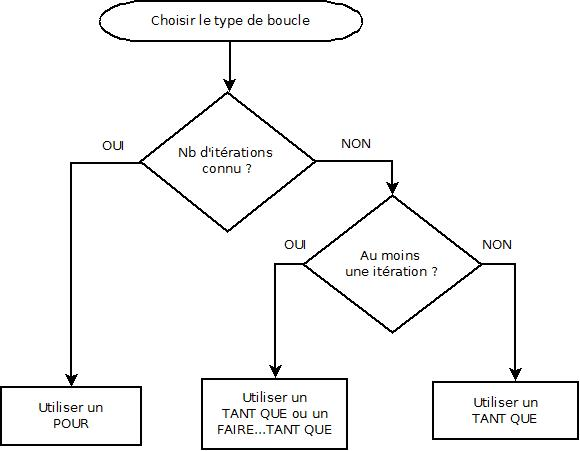
\includegraphics[width=.8\textwidth]{images/boucle-choixtype}
			\caption{Récapitulatif, choix d'une structure répétitive}
			\label{fig:boucle-choix}
		\end{figure}
	\end{center}




% ================================
\section{Exercices résolus}
% ================================

\subsection{Saisie des données par l'utilisateur}

	Il existe des problèmes où l’algorithme doit demander une série de valeurs
	à l’utilisateur pour pouvoir les traiter.  Par exemple, les sommer, en faire
	la moyenne, calculer la plus grande\dots
	
	Dans ce genre de problème, l'algorithme ou le programme stocke chaque valeur
	donnée par l’utilisateur dans une seule et même variable et la traite avant
	de passer à la suivante.  Prenons un exemple concret pour mieux comprendre.

	\begin{quote}
	Écrire un algorithme et un programme qui calcule et retourne 
	la somme d’une série de nombres donnés par l’utilisateur. 
	\end{quote}

	Il faut d’abord se demander comment l’utilisateur va pouvoir indiquer
	combien de nombres il faut additionner ou quand est-ce que le dernier nombre
	à additionner a été entré.  Voyons quelques possibilités.
	

	\subsubsection{Variante 1~: le nombre de valeurs est connu} 
	%-------------------------------------------------------	
	
		L’utilisateur indique le nombre de termes au départ.
		Ce problème est proche de ce qui a déjà été fait.
		
		En langage Java, l'habitude est de commencer à compter à partir de 0.
		Là où nous avons l'habitude de compter de $1$ à $n$, nous compterons
		toujours de $0$ à $n-1$. Plutôt que d'avoir comme condition de fin $i
		<= n - 1$, nous écrirons $i < n$.

		Une solution en Java peut-être~:

		\begin{java}
public static int sum(){
	int nValues;		// Nombre de valeurs à additionner
	int value;			// Terme de l'addition
	int sum = 0;		// Somme construite au fur et à mesure
	Scanner keyboard = new Scanner(System.in); // nécessite un import
	
	nValues = keyboard.nextInt();
	for  (int i = 0; i < nValues; i = i + 1){
		value = keyboard.nextInt();
		sum = sum + value;
	}
	return sum;
}
		\end{java}


		\paragraph{Remarque}

		Dans les exemples, nous utilisons des lectures au clavier très
		rudimentaires. Par exemple~:

		\begin{java}
value = keyboard.nextInt();			
		\end{java}

		Cette instruction, lorsqu'elle est exécutée, se traduit par un curseur
		qui clignote en attendant un nombre entier. Ce serait mieux de
		demander à l'utilisateur au préalable d'entrer un entier en lui écrivant
		un message. Plutôt comme suit~:

		\begin{java}
System.out.print("Entrer un entier: ");			
value = keyboard.nextInt();			
		\end{java}

		\texttt{nextInt} lit un entier au clavier. Si ce n'est pas un entier qui
		est entré… une erreur survient et le programme plante lamentablement.
		Pour éviter ceci, nous pouvons demander au programme de vérifier que
		l'utilisateur ou l'utilisatrice entre bien un entier, sinon, lui
		signaler. Justement la classe \texttt{Scanner} propose une méthode
		\texttt{hasNextInt}. Nous pourrions alors écrire ceci~:

		\begin{java}
System.out.print("Entrer un entier: ");			
while (!keyboard.hasNextInt()){
	keyboard.next();
}
value = keyboard.nextInt();						
		\end{java}

		Lors de l'appel à la méthode \texttt{hasNextInt}, l'utilisateur va
		devoir entrer une valeur qui sera mémorisée (\textit{bufferisée}) et la
		méthode retourne \texttt{true} si l'utilisateur a entré un entier,
		\texttt{false} sinon. 
		\begin{itemize}

			\item Si c'est \texttt{true}, c'est un entier. Le programme n'entre
				pas dans la boucle et se rend directement à l'instruction
				suivante. Cette instruction consomme la valeur lue précédemment
				et la place dans la variable \pc{value}.

			\item Si c'est \texttt{false}, ce n'est pas un entier. Le programme
				entre dans la boucle et l'instruction \texttt{keyboard.next()}
				consomme la valeur lue précédemment… et n'en fait rien. Elle
				vide simplement le \textit{buffer}. 

				Le programme retourne au test et réexécute \texttt{hasNextInt}
				qui lit une valeur au clavier et la place dans le
				\textit{buffer}. Et ainsi de suite. 

		\end{itemize}
			
	\subsubsection{Variante 2~: stop ou encore}
	%------------------------------------------------	
	
		Après chaque nombre, l'algorithme ou le programme demande
		à l’utilisateur s’il y a encore un nombre à additionner.

		Dans ce cas, il faut chercher une solution différente car le nombre de
		valeurs à additionner — et donc le nombre d’exécution de la boucle
		— n'est pas connu au départ. Il faudra utiliser un «~tant que~» ou un
		«~faire-tant~que~». 
		
		Si nous demandons en fin de boucle s’il reste encore un nombre
		à additionner l'algorithme aura l'allure suivante où nous utilisons un
		«~do~-~while~»~:

		\begin{java}
public static int sum(){
	/* Est-ce qu'il reste une variable à additionner (hasMore) */
	boolean hasMore;
	int value;
	int sum = 0;
	Scanner keyboard = new Scanner(System.in); // nécessite un import

	do {
		value = keyboard.nextInt();
		sum = sum + value;
		hasMore = keyboard.nextBoolean();
	} while (hasMore);
	return sum;
}
		\end{java}
		
		Avec cette solution, on additionne au moins une valeur.  Il est possible
		de tenir compte du cas particulier où l’utilisateur ne veut additionner
		aucune valeur. Dans ce cas, il faut utiliser un «~tant que~» et donc
		poser la question avant d’entrer dans la boucle.

		\begin{java}
public static int sum(){
	/* Est-ce qu'il reste une variable à additionner (hasMore) */
	boolean hasMore;
	int value;
	int sum = 0;
	Scanner keyboard = new Scanner(System.in); // nécessite un import

	hasMore = keyboard.nextBoolean();
	while (hasMore){
		value = keyboard.nextInt();
		sum = sum + value;
		hasMore = keyboard.nextBoolean();
	}
	return sum;
}
		\end{java}


	\subsubsection{Variante 3~: valeur sentinelle}
	\index{valeur sentinelle}
	%------------------------------------------------	
		
		L’utilisateur entre une valeur spéciale pour indiquer la fin. Il s'agit
		d'une valeur \textbf{sentinelle}. 
		
		Cette solution n'est envisageable que si cette valeur \textbf{sentinelle} 
		ne fait pas partie de l'ensemble des valeurs possibles. 
		
		Dans notre exemple si on veut additionner des nombres positifs
		uniquement, la valeur -1 peut servir de valeur sentinelle. Mais sans
		limite sur les nombres à additionner (positifs, négatifs ou nuls), il
		n’est pas possible de choisir une sentinelle.

		Ici, on se base sur la valeur entrée pour décider si on continue ou pas.
		Il faut donc \textbf{toujours} effectuer un test après une lecture de
		valeur. C’est pour cela qu’il faut effectuer une lecture avant la boucle
		et une autre à la fin de la boucle.

		\begin{java}
public static int sum(){
	int value;			// Un des termes de l'addition
	int sum = 0;		// La somme
	Scanner keyboard = new Scanner(System.in); // nécessite un import

	value = keyboard.nextInt();
	while (value != -1){
		sum = sum + value;
		value = keyboard.nextInt();
	}
	return sum;
}	
		\end{java}

% ================================
\subsection{Les suites}
\label{chap:suites}
% ================================

	Nous avons vu quelques exemples d’algorithmes qui affichent une suite de
	nombres (par exemple, afficher les nombres pairs).  Nous avons pu les
	résoudre facilement avec un \pc{\algorithmicfor} en choisissant
	judicieusement les valeurs de début et de fin ainsi que le pas.
	
	Ce n’est pas toujours aussi simple.  Nous allons voir deux exemples plus
	complexes et les solutions qui les accompagnent.  Elles pourront se
	généraliser à beaucoup d’autres exemples.
	
	\subsubsection{Exemple 1 - Afficher les carrés}
	%--------------------------------------------
	
		Nous voulons afficher les $n$ premiers nombres carrés parfaits~:
		$1$, $4$, $9$, $16$, $25$\dots

		Si l'on veut savoir quel est le 7\ieme{} nombre à afficher, c'est $7^2$,
		soit $49$.  Plus généralement, le nombre à afficher lors du $i$\ieme{}
		passage dans la boucle est $i^2$.

		\begin{tabular}{l|*{8}{>{\centering\arraybackslash}m{3mm}}}
		 étape & 1 & 2 & 3 & 4 & 5 & 6 & 7 & 8\\\hline
		 valeur à afficher & 1 & 4 & 9 & 16 & 25 & 36 & 49 & 64 \\
		\end{tabular}
		
		L’algorithme qui en découle est~:

		\begin{java}
public static void squarres(int n){
	for (int i = 1; i <= n; i++){
		System.out.printl(Math.pow(i, 2));
	}
}
		\end{java}

		Dans cette solution, la variable de contrôle compte simplement le nombre
		d’itérations.  Le calcul du nombre à affiche se fait en fonction de
		cette variable de contrôle (ici le carré convient).
		Par une vieille habitude des programmeurs%
		\footnote{%
			Née avec le langage FORTRAN 
			où la variable $i$ était par défaut une variable entière.
		},
		une variable de contrôle qui se contente de compter les passages dans la
		boucle est souvent nommée $i$. Elle es appelée «~indice~» de parcours de
		la boucle.	

		Cette solution peut être utilisée chaque fois qu’on peut calculer le
		nombre à afficher en fonction de $i$.
		
		Cet exemple illustre un premier modèle important d'algorithme de
		génération de suite, modèle dans lequel l'élément à la i\ieme\ place,
		souvent appelé le \textit{i\ieme\ terme}, peut être déterminé
		directement au départ d'une fonction de l'indice i.

		\[
			i \longrightarrow f(i)
		\]
		 	 
	\subsubsection{Exemple 2 - Une suite un peu plus complexe}
	%-------------------------------------------------------
	 
		Écrire un algorithme qui affiche les $n$ premiers nombres de la suite~:
		1, 2, 4, 7, 11, 16\dots{}
		
		Comme nous pouvons le constater, 
		à chaque étape on ajoute un peu plus au nombre précédent.
		\[ 
			1 
			\xrightarrow{+1} 2 
			\xrightarrow{+2} 4
			\xrightarrow{+3} 7 
			\xrightarrow{+4} 11 
			\xrightarrow{+5} 16 
			\dots
		\] 

		Ici, difficile de partir de la solution de l’exemple précédent car il
		est n’est pas facile de trouver la fonction $f(i)$ qui permet de
		calculer le nombre à afficher en fonction de i. 
		
		Par contre, il est assez simple de calculer ce nombre 
		en fonction du précédent.
		\[
			\mbox{nb à afficher} = \mbox{nb affiché juste avant} + i
		\]
		
		Sauf pour le premier, qui ne peut pas être calculé en fonction du
		précédent.

		Mathématiquement, cette suite s'écrirait

		\begin{align*}
			x_0 &= 1\\
			x_i &= x_{i-1} + i
		\end{align*}


		Une solution élégante et facilement adaptable à d’autres situations
		est~:

		\begin{langagenaturel}
			value = première valeur à afficher\\
			for i de 1 à n\\
			\tab print value\\
			\tab value = valeur suivante calculée à partir de la précédente
		\end{langagenaturel}
		
		
		qui, dans notre exemple précis, devient~:

		\begin{java}
public static void suite(int n){
	int value = 1;
	for (int i=1; i <= n; i = i + 1){
		System.out.println(value);
		value = value + 1;
	}
}
		\end{java}

		Cet exemple illustre un second modèle de génération de suite dans lequel
		l'élément à la i\ieme\ place, le i\ieme\ terme, est exprimé en fonction
		du ou des précédents termes. Ce genre de suite, s'appelle  «~suite
		récurrente~». 
		\index{suite récurrent}
                     

		% ============================
%\chapter{Les tests}
\renewcommand{\chaptername}{Errata}
\chapter{Les tests}
\label{chap:tests}
% ============================

\begin{Exergue}
	«~J'ai fait tourner le programme, il fonctionne bien.~»
\end{Exergue}

Tous les programmes contiennent des erreurs, des \textit{bugs}, des défauts… Ces
«~\textit{bugs}~» entrainent, au mieux, un inconfort pour l'utilisateur ou
l'utilisatrice. Ils peuvent occasionner une perte de temps, d'argent, de
données, de matériel… ou, pire, un danger pour la vie humaine dans un
environnement industriel par exemple. 

Le travail de développeur ou de la développeuse est de réduire le nombre
d'erreurs dans son programme. Pour ce faire, il ou elle le \textbf{testera}
abondamment.  Ce chapitre s'intéresse aux tests. 

\minitoc


\section{Les types d'erreurs et de tests}

Les défauts d'un programme peuvent être de différentes sortes:

\begin{enumerate}
	
	\item les erreurs de compilation~;

		Ces erreurs sont détectées par le compilateur et rapidement corrigées.

	\item les erreurs d'exécution
		
		… et le programme s'arrête~;


		… et le programme ne fournit pas les bonnes valeurs~;

		Ces erreurs sont difficiles à corriger. Elles nécessitent
		que le programme soit \textbf{testé} avec un nombre suffisant de
		situations différentes. Elles peuvent être dues à des erreurs de
		programmation mais aussi à des erreurs dans nos algorithmes. 

	\item les erreurs de programmation qui entrainent une lenteur du programme 
		ou une consommation excessive de mémoire. 

		Pour éviter ces erreurs, respecter les bonnes pratiques de développement
		est une première étape qu'il ne faut pas négliger. Ensuite, il faudra
		détecter les endroits dans le code où les ralentissements ont lieu ou la
		consommation de mémoire augmente. Il existe des logiciels dédiés à ce
		genre de cas. 

\end{enumerate}

Pour montrer — garantir, prouver — qu'un programme fonctionne bien, il ne suffit
pas de montrer qu'il fournit les bons résultats dans certains cas, il faut
convaincre, qu'il fournira les bons résultats dans \textbf{tous} les cas:

\begin{itemize}
	\item les cas généraux;
	\item les cas particuliers;
	\item lors d'une défaillance de l'environnement;
		
		Par exemple, si un capteur de distance est défectueux, il faut que la 
		chaine de production s'arrête. 
	
	\item lors d'une utilisation non conforme du programme.
\end{itemize}

Pour répondre à ces attentes, le développeur ou la développeuse sera attentif·ve
à utiliser une méthodologie éprouvée dans toutes les étapes de développement de
son projet; de la phase d'analyse au déploiement.  Il mettra en place différents
types de tests
\footnote{Voir \url{https://fr.wikipedia.org/wiki/Test_(informatique)}}
; des tests unitaires, d'intégration, fonctionnels, de non-régression… Dans ce
premier cours de développement, nous nous intéressons aux \textbf{tests
unitaires}.  Pour ces tests unitaires, le développeur ou la développeuse
fournira un ensemble de valeurs à tester représentatives et convaincantes. 

\index{test unitaire}
\marginicon{definition}
\textbf{Définition}

\textbf{Test unitaire} Procédure permettant de tester le bon fonctionnement d'un
module, d'une méthode. En fonction des paramètres qu'elle reçoit en entrée, la
méthode fournit elle les bons résultats ? 

L'idée sous-jacente des tests unitaires est que si chaque partie est correcte,
l'ensemble sera correct. 

Pour tester régulièrement — très régulièrement — notre programme nous avons besoin
d'outils qui vont automatiser ces tests mais commençons par les planifier. 


\section{Planifier les tests}

Dans la méthode de résolution de problèmes que nous avons présenté dans le chapitre \ref{refpblm} p.\pageref{refpblm} et dans l'exercice résolu de la section \ref{exerciceresolu} p.\pageref{exerciceresolu} nous précisions que l'écriture d'une solution complète dans ce premier cours de développement consistait en: 

\begin{enumerate}
	\item spécifier le problème;
	\item fournir des exemples;
	\item écrire un algorithme;
	\item vérifier les exemples (en traçant l'algorithme);
	\item écrire un programme correspondant à l'algorithme;
	\item tester le programme et constater qu'il fournit bien les résultats attendus.
\end{enumerate}

Les points 2 et 4 sont les prémisses à l'écriture des tests puisque ces exemples
vont nous convaincre que l'algorithme — et le programme — fournit bien les
«~bons~» résultats. Ces exemples constituent le \textbf{plan de tests} que nous allons utiliser. Dans ces différents cas, outre les cas généraux, les cas particuliers, les valeurs limites, apparaitront aussi des cas montrant les erreurs de programmation fréquentes. Par exemple~:

\begin{itemize}
	\item commencer ou arrêter trop tôt ou trop tard une boucle;
	\item ne pas initialiser ou mal initialiser une variable;
	\item confondre < et $\le$ ou > et $\ge$… voire < et >;
	\item confondre AND et OR;
	\item mal écrire la négation d'une proposition;
	\item …
\end{itemize}

C'est l'expérience qui permettra d'écrire un plan de tests efficace et
convaincant.

\paragraph{Remarque} Dans certaines méthodologies, la mise en exergue de l'importance des tests se fait en écrivant d'abord les tests avant le code.
Voir par exemple \href{https://fr.wikipedia.org/wiki/Test_driven_development}{Wikipedia} ou \href{http://www.extremeprogramming.org/rules/testfirst.html}{cette article d'\textit{extreme programming}}. 

Dès lors que le plan de tests est écrit, nous pouvons nous intéresser aux outils
qui vont permettre d'automatiser l'exécution des tests et faciliter leur
écriture.  En effet pour que nos tests soient utiles il faudra tester souvent
— idéalement dès qu'une méthode est écrite — et «~tout~». Ce sont toutes les
méthodes qui sont testées parce que l'écriture d'une méthode pourrait amener une
erreur dans une autre méthode. Dans ces conditions, pour que le développeur ou
la développeuse teste son programme, ce doit être automatique.  

Cette automatisation est fournie par \text{JUnit}.

\section{JUnit}

\paragraph{Remarque préalable} JUnit n'est pas fourni avec le JDK (\textit{java
development kit}), c'est un \textit{framework} de tests indépendant que l'on
trouve sur \url{junit.org}. Il est donc nécessaire de l'installer. 

Par contre, il est fourni avec Netbeans. 

\index{junit}
\marginicon{definition}
\textbf{JUnit} est un \textit{framework} simple pour l'écriture de tests
répétables. 

Pour tester la méthode — \texttt{foo} — dans la classe \texttt{MyClass}, il faut
écrire une classe \texttt{MyClassTest} qui contiendra les méthodes de tests et
demander à JUnit — dès lors qu'il est installé — d'exécuter cette classe. Un clic dans un IDE ou une commande du style fait l'affaire~:

\begin{term}
	java org.junit.runner.JUnitCore my.package.MyClassTest
\end{term}

La classe \texttt{MyClassTest} contient plusieurs méthodes. Une méthode de test
par cas. Une méthode de test~: 

\begin{itemize}
	\item est autonome. Elle ne reçoit pas de paramètre et ne retourne rien;
	
	\item contient des affirmations qui seront évaluées;

		\textit{La méthode doit me retourner «~vrai~».}~: \pc{assertTrue()}\\
		\textit{La méthode doit me retourner «~faux~».}~: \pc{assertFalse()}\\
		\textit{La méthode doit me donner cette valeur si ses paramètres sont
		ceux-ci.}~:\\\pc{assertEqauls(<valeur attendue>, <valeur>)}

	\item est précédée de l'annotation \pc{@Test} permettant de la faire
		reconnaitre comme un test unitaire;

	\item n'a pas de mot clé \pc{static}.

\end{itemize}

Un test aura donc l'allure suivante~:

\begin{java}
@Test
public void max2_cas1(){
	assertEquals(2, max2(-1, 2));
}
\end{java}

Après lancement des tests, JUnit fournirait un rapport l'allure suivante~:

\begin{term}
JUnit version 4.12
.

Time: 0,012

OK (1 test)
\end{term}

\section{Exemple}

Reprenons l'exemple du calcul du maximum de 2 nombres décrit dans la fiche
\ref{fiche:max2nb} p.\pageref{fiche:max2nb}. Voici un plan de tests~:

\begin{center}
\begin{tabular}{|c|cc|c|}
	\hline
	\rowcolor{black!40}
	test \no & nb1 & nb2 & réponse attendue  \\
	\hline 
	1 & -3    & 4   & 4	\\\hline
	2 & 7     & 4   & 7 \\\hline
	3 & 4     & 4   & 4 \\\hline
	4 & 0     & -4  & 0 \\\hline
\end{tabular}
\end{center}		

Et la classe de tests \texttt{MaximumTest} sans les commentaires.

\begin{java}
package esi-bru.cours.dev1;

import org.junit.Test;
import static org.junit.Assert.*;

public class MaximumTest {
    
    
	@Test
	public void max2_cas1(){
		assertEquals(4, max2(-3, 4));
	}

	@Test
	public void max2_cas2(){
		assertEquals(7, max2(7, 4));
	}

	@Test
	public void max2_cas3(){
		assertEquals(4, max2(4, 4));
	}

	@Test
	public void max2_cas4(){
		assertEquals(0, max2(0, -4));
	}
}
\end{java}


\begin{term}
JUnit version 4.12
....

Time: 0,012

OK (4 tests)
\end{term}








	\part{Les tableaux}
	%----------------------------------------------------------
		%======================
\chapter{Les tableaux}
\label{chap:tableaux}
%======================

	Dans ce chapitre nous étudions les tableaux, une structure qui peut contenir
	plusieurs exemplaires de même type.

	\minitoc
	\clearpage
	% =============================
	\section{Utilité des tableaux}
	% =============================
	
		Nous allons introduire la notion de tableau à partir d’un exemple 
		dans lequel l’utilité de cette structure de données 
		apparaitra de façon naturelle.
	
		\textbf{Exemple.}
		Statistiques de ventes.
		\begin{quote}	
		
			Un gérant d’une entreprise commerciale souhaite connaitre l’impact
			d’une journée de promotion publicitaire sur la vente de dix de ses
			produits.  
			
			Pour ce faire, les numéros de ces produits (numérotés de
			0 à 9 pour simplifier) ainsi que les quantités vendues pendant cette
			journée de promotion sont encodés au fur et à mesure de leurs
			ventes.  En fin de journée, le vendeur entrera la valeur -1 pour
			signaler la fin de l’introduction des données.  Ensuite, les
			statistiques des ventes seront affichées.
		
		\end{quote}

		La démarche générale se décompose en trois parties~:
		\begin{itemize}
		
			\item le traitement de début de journée, qui consiste
				essentiellement à mettre les compteurs des quantités vendues
				pour chaque produit à 0~;
		
			\item le traitement itératif durant toute la journée~: au fur et
				à mesure des ventes, il convient de les enregistrer,
				c’est-à-dire d’ajouter au compteur des ventes d’un produit la
				quantité vendue de ce produit~; ce traitement itératif
				s’interrompra lorsque la valeur -1 sera introduite~;
		
			\item le traitement final, consistant à communiquer les valeurs des
				compteurs pour chaque produit.
		
	\end{itemize}
	
		Vous trouverez sur la page suivante une version possible de cet
		algorithme sans utiliser les tabeaux.

		\begin{java}
import java.util.Scanner;
/*
 Calcule et affiche la quantité vendue de 10 produits
*/
public static void statistics(){
	Scanner keyboard = new Scanner(System.in);
	int cpt0, cpt1, cpt2, cpt3, cpt4, cpt5, cpt6, cpt7, cpt8, cpt9;
	int productId, quantity;
	cpt0 = 0;
	cpt1 = 0;
	cpt2 = 0;
	cpt3 = 0;
	cpt4 = 0;
	cpt5 = 0;
	cpt6 = 0;
	cpt7 = 0;
	cpt8 = 0;
	cpt9 = 0;
	System.out.print("Introduire le numéro de produit : ");
	productId = keyboard.nextInt();
	while (productId != -1){
		System.out.print("Quantité:");
		quantity = keyboard.nextInt();
		switch (productId){
			case 0:
				cpt0 = cpt0 + quantity;
				break;
			case 1:
				cpt1 = cpt1 + quantity;
				break;
			case 2:
				cpt2 = cpt2 + quantity;
				break;
			case 3:
				cpt3 = cpt3 + quantity;
				break;
			case 4:
				cpt4 = cpt4 + quantity;
				break;
			case 5:
				cpt5 = cpt5 + quantity;
				break;
			case 6:
				cpt6 = cpt6 + quantity;
				break;
			case 7:
				cpt7 = cpt7 + quantity;
				break;
			case 8:
				cpt8 = cpt8 + quantity;
				break;
			case 9:
				cpt9 = cpt9 + quantity;
				break;
		}
		System.out.print("Introduire le numéro de produit : ");
		productId = keyboard.nextInt();
	}

	\end{java}
	
	\begin{java}

	System.out.println("Quantité vendue de produit 0" + cpt0);
	System.out.println("Quantité vendue de produit 1" + cpt1);
	System.out.println("Quantité vendue de produit 2" + cpt2);
	System.out.println("Quantité vendue de produit 3" + cpt3);
	System.out.println("Quantité vendue de produit 4" + cpt4);
	System.out.println("Quantité vendue de produit 5" + cpt5);
	System.out.println("Quantité vendue de produit 6" + cpt6);
	System.out.println("Quantité vendue de produit 7" + cpt7);
	System.out.println("Quantité vendue de produit 8" + cpt8);
	System.out.println("Quantité vendue de produit 9" + cpt9);
 }
		\end{java}
	

		\index{tableau}
		Que se passerait-il si le nombre de produits à traiter était de 20, voire
		1000~? Une simplification de l'écriture s'impose.  La solution est
		apportée par un nouveau type de variables~: les \textbf{variables
		indicées} ou \textbf{tableaux} (\textit{arrays} en anglais).
	
		Au lieu d’avoir à manier dix compteurs distincts
		(\pc{cpt0}, \pc{cpt1}, etc.), 
		nous allons envisager une seule «~grande~» variable 
		\pc{cpt} compartimentée en dix «~cases~» ou «~sous-variables~»
		(appelées aussi les «~éléments~» du tableau). 
		Elles se distingueront les unes des autres par un numéro 
		(un «~indice~»)~: 
		\pc{cpt0} deviendrait ainsi \pc{cpt[0]}, 
		\pc{cpt1} deviendrait \pc{cpt[1]}, 
		et ainsi de suite jusqu’à
		\pc{cpt9} qui deviendrait \pc{cpt[9]}.
	
		\begin{center}
			\begin{tabular}{*{11}{>{\centering\arraybackslash}m{5mm}}}
				{} &
				\pc{cpt[0]} &
				\pc{cpt[1]} &
				\pc{cpt[2]} &
				\pc{cpt[3]} &
				\pc{cpt[4]} &
				\pc{cpt[5]} &
				\pc{cpt[6]} &
				\pc{cpt[7]} &
				\pc{cpt[8]} &
				\pc{cpt[9]} 
				\\\hhline{~*{10}{-}}
				\multicolumn{1}{m{5mm}|}{\pc{cpt}} &
				\multicolumn{1}{m{5mm}|}{~} &
				\multicolumn{1}{m{5mm}|}{~} &
				\multicolumn{1}{m{5mm}|}{~} &
				\multicolumn{1}{m{5mm}|}{~} &
				\multicolumn{1}{m{5mm}|}{~} &
				\multicolumn{1}{m{5mm}|}{~} &
				\multicolumn{1}{m{5mm}|}{~} &
				\multicolumn{1}{m{5mm}|}{~} &
				\multicolumn{1}{m{5mm}|}{~} &
				\multicolumn{1}{m{5mm}|}{~}
				\\\hhline{~*{10}{-}}
			\end{tabular}
		\end{center}
	
		Un des intérêts de cette notation est la possibilité de faire apparaitre
		une variable entre les crochets, par exemple \pc{cpt[i]}, ce qui permet
		une grande économie de lignes de code.
		
		Voici la version de notre solution avec tableau.
	
		\label{tableau:tab1DStock10Articles}
		\begin{java}
import java.util.Scanner;
public static void statisticsWithArray(){
	Scanner keyboard = new Scanner(System.in);
	int[] cpt = {0, 0, 0, 0, 0, 0, 0, 0, 0, 0};
	int i;
	int productId;
	int quantity;
	System.out.print("Introduire le numéro de produit : ");
	productId = keyboard.nextInt();
	while (productId != -1){
		System.out.print("Quantité:");
		quantity = keyboard.nextInt();
	
		cpt[productId] = cpt[productId] + quantity;

		System.out.print("Introduire le numéro de produit : ");
		productId = keyboard.nextInt();		
	}

	for(int i=0; i<10; i++){
		System.out.println("Quantité vendue de produit " i + ": " + cpt[i]);		
	}
}
			
		\end{java}

		
	% ====================
	\section{Définitions}
	% ====================
	
		\marginicon{definition}\index{tableau}
		Un \textbf{tableau} est une suite d’éléments de même type 
		portant tous le même nom mais se distinguant 
		les uns des autres par un indice.
	
		L’\textbf{indice} est un entier\index{tableau (indice)}
		donnant la position d’un élément dans la suite. 
		Cet indice varie entre la position du premier élément 
		et la position du dernier élément, 
		ces positions correspondant aux bornes de l’indice.
		Notons qu’il n’y a pas de «~trou~»~: 
		tous les éléments existent entre le premier et le dernier indice.
	
		La \textbf{taille} d’un tableau\index{tableau (taille)} est le nombre de
		ses éléments.  Attention, la taille d’un tableau ne peut pas être
		modifiée pendant son utilisation, elle est déterminée à la création du
		tableau.

		Un tableau est de type \textbf{référence}\index{référence}.
	
	% ======================================================
	\section{Déclaration - création - initialisation}
	\label{sec:tableaudci}
	% ======================================================

		\marginicon{definition}
		Afin de pouvoir utiliser un tableau, il sera nécessaire de distinguer~:
		\begin{itemize}

			\item la \textbf{déclaration} qui consiste à signaler qu'une
				variable est un tableau. Dans un programme, cette déclaration
				a pour effet de réserver un emplacement mémoire qui contiendra
				une référence vers les cases du tableau\,; 

			\item la \textbf{création} du tableau consiste a réserver
				l'emplacement mémoire qui contiendra les différentes valeurs.
				Pour le créer, il faut connaitre sa taille\,; 

			\item l'\textbf{initialisation} du tableau consiste à donner ses
				premières valeurs aux différents éléments du tableau.
		
		\end{itemize}


		\index{déclaration}
		\index{création}
		Nous supposerons dans la suite que \pc{length} est le nombre d’éléments
		—~la longueur~—
		et \pc{Type} est le type des éléments que l’on trouvera dans le tableau.  
		
		Tous les types sont permis mais tous les éléments sont du même type. 

		\subsection{Déclaration}
		\index{déclaration}

		Pour \textbf{déclarer} un tableau~:

	\begin{grammaire}
		\grammarrule{ArrayDeclarationExpression:}
		    \grammarrule{Type}[] \grammarrule{Identifier}
	\end{grammaire}

	\begin{java}
int[] myArray;
String[] strings;
	\end{java}

	Seule la variable est déclarée. Aucun espace mémoire n'est réservé pour
	recevoir les éléments du tableau. Ceci sera fait lors de la création du
	tableau.  

	\subsection{Création}
	\index{création}
		
	Pour \textbf{créer} un tableau, préalablement déclaré, nous écrirons~:

	\begin{grammaire}
		\grammarrule{ArrayCreationExpression:}
		    new \grammarrule{Type}[\grammarrule{Expression}]
	\end{grammaire}

	\begin{java}
myArray = new int[10];
strings = new String[3];
	\end{java}

	L'emplacement mémoire nécessaire pour stocker la valeur de chaque élément
	du tableau est réservé. 

	\subsection{Initialisation}
	\index{initialisation}

	Pour \textbf{initialiser} les éléments du tableau, nous pouvons le faire en
	accédant à chaque élément du tableau. Un par un. 
	
	L'accès aux éléments d'un tableau se fait grâce aux crochets
	\pc{myArray[i]} pour nos algorithmes, en langage Java et dans beaucoup
	d'autres langages. Comme suit~:

	\begin{java}
		myArray[0] = 5;
		strings[1] = "Hello";
	\end{java}

	La première case du tableau porte l’indice \pc{0}
	la dernière l’indice \pc{size-1}.  C’est une erreur
	d’indiquer un indice qui ne correspond pas à une case du tableau (trop petit
	ou trop grand).  Par exemple, si on déclare et crée le tableau \pc{myArray}~:

	\begin{java}
int[] myArray = new int[100];
	\end{java}
	c'est une erreur d’utiliser \pc{myArray[-1]} ou \pc{myArray[100]}. 

	Il est également possible d'initialiser un tableau en une seule fois, en 
	utilisant un \textit{array initializer}. Une notation entre accolades. 

	\begin{langagenaturel}
myArray = \{2, 3, 7\}
	\end{langagenaturel}

	Voici la grammaire Java. 

	\begin{grammaire}
		\grammarrule{ArrayInitializer:}
		    \{ \grammarrule{[VariableInitializerList]} \}

		\grammarrule{VariableInitializerList:}
		    \grammarrule{Expression} \grammarrule{[}, \grammarrule{Expression ]} 
	\end{grammaire}

	\begin{java}
		int[] myArray;
		myArray = new int[3];
		myArray[0] = 2;
		myArray[1] = 3;
		myArray[2] = 7;

		myArray = new int[] {-1, 3, 12, 5};

		int[] myArray2 = {3, 14, 15, 92};
		
	\end{java}

	\begin{description}

		\item[ligne 7] Pour utiliser un \textit{ArrayInitializer}, il faut créer
			et initialiser le tableau dans la même instruction. Dans ce cas, le
			langage interdit de renseigner le nombre d'éléments du tableau… le
			compilateur peut le déduire.

			Cette instruction crée un nouveau tableau qui écrase l'autre. 

		\item[ligne 9] Lorsque l'on initialise le tableau avec un
			\textit{ArrayInitializer} lors de la déclaration, la partie création
			peut être omise.
	
	\end{description}

	\paragraph{Remarque.} Chaque élément d’un tableau doit être manié avec la
	même précaution qu’une variable simple, c’est-à-dire qu’on ne peut utiliser
	un élément du tableau qui n’aurait pas été préalablement affecté ou
	initialisé.

		

	% ==============================
	\section{Tableau et paramètres}
	% ==============================
	
		Le type \emph{tableau} étant un type à part entière, il est tout-à-fait
		éligible comme type pour les paramètres et la valeur de retour d’un
		algorithme.  De manière générale là où pouvait apparaitre un type
		(entier, pseudo-réel…) peut apparaitre un tableau.  Toujours.  Voyons
		cela en détail.  

		Nous avons vu dans la section \ref{paramètres} p.~\pageref{paramètres}
		les différentes sortes de paramètres. Voyons ce qu'il en est pour
		chacun d'eux lorsque ce paramètre est un tableau. 


		\subsection{Un tableau comme paramètre en entrée}
				
		\In : indique que l’algorithme va consulter les valeurs du tableau reçu
		en paramètre.  Les éléments doivent donc avoir été initialisés avant
		d’appeler l’algorithme. Exemple~:
			
		\begin{pseudocode}
			\LComment{Affiche les éléments d’un tableau}
			\Algo{display}{\Par{myArray\In}{\Array{10}{integers}}}{} 
				\For{i}{0}{9}
					\Write myArray[i]
				\EndFor
			\EndAlgo 

			\Empty
			\LComment{Utilisations possible}
			\Decl{anArray}{\Array{10}{integers}}
			\Let anArray \Gets \{2,3,5,7,11,13,17,19,23,29\}
			\Stmt display(anArray)
		\end{pseudocode}
	

		\subsection{Un tableau comme paramètre en entrée-sortie}

		\In\Out : indique que l’algorithme va consulter/modifier les valeurs du
		tableau reçu en paramètre. Exemple~:
			
		\begin{pseudocode}
			\LComment{Inverse le signe des éléments du tableau}
			\Algo{reverseSigne}{\Par{myArray\In\Out}{\Array{10}{integers}}}{} 
				\For{i}{0}{9}
					\Let myArray[i] \Gets -myArray[i]
				\EndFor
			\EndAlgo 

			\Empty
			\LComment{Utilisation possible}
			\Decl{anArray}{\Array{}{integers}}
			\Let anArray \Gets	
				{\Array{}{integers}}
				\{2,-3,5,-7,11,13,17,-19,23,29\}
			\Stmt reverseSigne(anArray)
		\end{pseudocode}


		\subsection{Un tableau comme paramètre en langage Java}

		En langage Java, le passage de paramètres se fait toujours par valeur.
		Comme un tableau est de type référence, c'est bien la valeur de la
		référence qui est passée en paramètre. En ce sens, il sera possible de
		modifier les valeurs d'un tableau reçu mais pas de remplacer le tableau
		reçu par un autre. Exemples~:

\begin{java}
	public static void reverseSigne(int[] is){
		for (int i=0; i < is.length; i = i + 1){
			is[i] = -is[i];
		}
	}

	// Utilisation
	int[] myArray = {2,-3,5,-7,11,13,17,-19,23,29};
	reverseSigne(myArray);
\end{java}

\marginicon{dont}
\begin{java}
	public static void fail(double[] ds){
		ds = new double[] {2, 2.61};
	}


	// Utilisation
	double[] myArray = {1, 3.14};
	fail(myArray);
	// 3.14 et pas 2.61
	System.out.println("Value: " + myArray[1]);		

\end{java}



		\subsection{Un tableau comme type de retour}

		Comme pour n’importe quel autre type, un algorithme ou un programme peut
		retourner un tableau.  Ce sera à lui de le déclarer et de lui donner des
		valeurs.  Exemple~:
			

\begin{java}
	public static int[] create(){
		int[] myArray = new int[10];
		for (int i=0; i < 10; i = i + 1){
			myArray[i] = i;
		}
		return myArray;
	}


	// Utilisation possible
	int[] anArray = create();
\end{java}

		\subsection{Paramétrer la taille}
		%---------------------------------
		
		Un tableau connait sa taille dès lors qu'elle existe c'est-à-dire dès
		que le tableau est créé. La taille est accessible grâce au mot
		\pc{length} comme suit~:

		\begin{java}
			double[] myArray;
			int size = myArray.length;

			double[] otherArray = {3.14, 2.71};
			int otherSize = otherArray.length;
		\end{java}

		Un tableau peut être passé en paramètre à un algorithme ou à une méthode
		et ce, quelle que soit la taille du tableau passé en paramètre.
		L'algorithme ou la méthode aura comme paramètre un tableau qui connait
		sa taille. Lorsque l'algorithme ou la méthode recevra le paramètre
		effectif, la taille sera déterminée. 
		
		\textbf{Exemple~:}

		\begin{java}
public static void display(int[] myArray){
	System.out.println("Tableau de " 
		+ myArray.length 
		+ " éléments." );
	for (int i=0; i< myArray.length; i++){
		System.out.println(myArray[i]);
	}

	// Utilisations possibles
	int[] integers = new int[2];
	integers[0] = 56;
	integers[1] = -3;
	display(integers);
	
	int[] myBeautifulArray = {6, 12, 18};
	display(myBeautifulArray);
}
		\end{java}

		La fiche \vref{fiche:tab-passage-param} récapitule tout ça.

	% ==============================================
	\section{Parcours d’un tableau} 
	\label{Les parcours de tableaux}
	% ==============================================

		Dans la plupart des problèmes que vous rencontrerez vous serez amenés
		à parcourir un tableau.  Il est important de maitriser ce parcours.
		Examinons les situations courantes et voyons quelles solutions
		conviennent.
	
		\begin{description}

			\item[Parcours complet]
		
			Nous avons déjà vu dans les exemples comment parcourir tous les
			éléments d’un tableau.  Une boucle \pc{for} fait généralement
			l'affaire comme ceci~:

			\begin{java}
int[] myArray = { /* insert values */ };
for (int index = 0; index < myArray.length; index++){
	// do something with myArray[index]
}
			\end{java}

			Java propose une autre forme de \pc{for} —~l'\textit{enhanced for}
			ou \textit{foreach}\index{foreach}~— permettant de parcourir un
			tableau\footnote{Nous verrons en DEV2, que cette structure permet
			de parcourir d'autres choses que les tableaux.}

			\begin{java}
int[] myArray = { /* insert values */ };
for (int value: myArray){
	// do something with value
}
			\end{java}
			
			La fiche \vref{fiche:tab-parcours-complet} décrit
			comment afficher tous les éléments d’un tableau.  Il est possible de
			faire autre chose avec ces éléments~: les sommer, les comparer\dots

			\item[Parcours partiel]
		
			Parfois, il n'est pas nécessaire de parcourir le tableau jusqu’au
			bout car un arrêt prématuré survient dès qu'une condition est
			remplie. 
			
			Par exemple~: recherche d'un élément et arrêt dès qu'il est trouvé~;
			vérification que toutes les valeurs sont non nulles mais l'on vient
			d'en trouver une~; vérification que la suite des éléments est
			positives alors que l'on vient d'en trouver un négatif ou nul.
	
			Pour résoudre ce problème, la structure \pc{tant que} avec un test
			d'arrêt fait bien l'affaire. 
			
			La fiche \vref{fiche:tab-parcours-partiel} détaille un parcours
			partiel.
	
		\end{description}
	
	% ==============================================
	\section{Taille logique\index{taille logique} et 
	taille physique\index{taille physique}} 
	% ==============================================

		Parfois, la taille du tableau n'est pas connue à l'avance.
		
		Imaginons, par exemple, qu’il s’agisse de demander des valeurs
		à l’utilisateur et de les stocker dans un tableau pour un traitement
		ultérieur.  Supposons que l’utilisateur va indiquer la fin des données
		par une valeur sentinelle.  Impossible de savoir, à priori, combien de
		valeurs il va entrer et, par conséquent, la taille à donner au tableau.
		
		Une solution est de créer un tableau suffisamment grand
		pour tous les cas%
		\footnote{%
			En tout cas, 
			suffisamment grand pour tous les cas qu’on accepte
			de prendre en compte; il faudra bien fixer une limite.
		} 
		quitte à n’en n’utiliser qu’une partie.
		
		Mais comment savoir quelle est la partie du tableau
		qui est effectivement utilisée~?
		
		Comprenez bien qu’il \textbf{n’y a pas de concept de case vide}.  Rien
		ne différencie une case utilisée d’une case non utilisée.  La manière de
		s'en sortir est de stocker les valeurs dans la partie basse du tableau
		(à gauche) et de retenir dans une variable le nombre de cases
		effectivement utilisées.
			
		\marginicon{definition}
		La \textbf{taille physique} d’un tableau 
		est le nombre de cases qu’il contient.
		Sa \textbf{taille logique}
		est le nombre de cases actuellement utilisées.
	
		\paragraph{Exemple.}
		Voici un tableau qui ne contient pour l’instant que quatre nombres.
		\begin{center}
			\begin{tabular}{*{10}{|>{\centering\arraybackslash}m{5mm}}|}
				\hline
				10 & 4 & 3 & 7 & ? & ? & ? & ? & ? & ? \\
				\hline
			\end{tabular}
			\\\medskip
			\pc{taillePhysique = 10}
			\qquad
			\pc{tailleLogique = 4}
		\end{center}

		Les cases indiquées par "?" ne sont pas vides~;
		elles peuvent être non initialisées
		(et il n'est pas possible de tester si une case est non initialisée)
		ou bien contenir une valeur qui n’est pas pertinente.
		
		\paragraph{Exemple.}
		L’algorithme suivant demande des valeurs positives à l’utilisateur et
		les stocke dans un tableau (maximum 1000).  Toute valeur négative ou
		nulle est une valeur sentinelle.

		\begin{java}
public static void stockValues(){
	Scanner keyboard = new Scanner(System.in);
	int[] myArray = new int[1000];
	int nbValues = 0;
	int value;
	value = keyboard.nextint();
	while (value > 0 && nbValues < myArray.length){
		myArray[nbValues] = value;
		nbValues++;
		value = keyboard.nextint();
	}
	// Test de value et pas de nbValues. Pourquoi ?
	if (value > 0){
		System.out.println("La limite physique a été atteinte");
	}
}			
		\end{java}
		
		En langage Java, essayer d'ajouter un élément en dehors de la taille du
		tableau va générer une erreur à l'exécution. Une
		\pc{ArrayIndexOutOfBoundException}. 

		
	% ==============================================
	\section{Les tableaux ont comme premier indice 0} 
	% ==============================================

		Les tableaux ont comme premier indice 0, Un tableau de taille \pc{n}
		a toujours ses indices allant de \pc{0} à \pc{n-1}. 

		Parfois le problème à résoudre donne envie d'avoir des indices dont le
		premier ne commence pas à 0. Par exemple allant de 1 à 7. Dans ces cas,
		il est toujours possible de s'arranger pour commencer à partir de 0. 

		\paragraph{Exemple.}
		Imaginons l’algorithme qui permet de convertir un numéro
		de jour en son intitulé~: 1 donne "lundi", 2 donne "mardi",
		\dots{}
		Une solution possible, sans tableau, serait~:
		
		\begin{java}
public static String dayName(int dayNumber){
	String dayName;
	switch (dayNumber){
		case 1:
			dayName = "lundi";
			break;
		case 2:
			dayName = "mardi";
			break;
		case 3:
			dayName = "mercredi";
			break;
		case 4:
			dayName = "jeudi";
			break;
		case 5:
			dayName = "vendredi";
			break;
		case 6:
			dayName = "samedi";
			break;
		case 7:
			dayName = "dimanche";
			break;
		default:
			dayName = "inconnu";
	}
	return dayName;
}
		\end{java}

		Mais une solution plus élégante passe par l’utilisation d’un tableau.
		Appelons-le \pc{dayString} et stockons-y les noms des jours
		comme illustré ci-dessous.

		\begin{center}
			\footnotesize
			\begin{tabular}{ccccccc}
				1 & 2 & 3 & 4 & 5 & 6 & 7
				\\\hline
				\multicolumn{1}{|c|}{"lundi"} &
				\multicolumn{1}{c|}{"mardi"} &
				\multicolumn{1}{c|}{"mercredi"} &
				\multicolumn{1}{c|}{"jeudi"} &
				\multicolumn{1}{c|}{"vendredi"} &
				\multicolumn{1}{c|}{"samedi"} &
				\multicolumn{1}{c|}{"dimanche"}
				\\\hline
			\end{tabular}
		\end{center}


		Si le tableau commence à l'indice 1 jusqu'à l'indice 7, pour obtenir le
		nom d’un jour, il suffirait d’écrire~: \pc{dayString[dayNumber]}.
		
		Comme les tableaux commencent toujours à l'indice 0, il faudra plutôt
		considérer le tableau ci-dessous et écrire \pc{dayString[dayNumber-1]}.
		
		\begin{center}
			\footnotesize
			\begin{tabular}{ccccccc}
				0 &1 & 2 & 3 & 4 & 5 & 6 
				\\\hline
				\multicolumn{1}{|c|}{"lundi"} &
				\multicolumn{1}{c|}{"mardi"} &
				\multicolumn{1}{c|}{"mercredi"} &
				\multicolumn{1}{c|}{"jeudi"} &
				\multicolumn{1}{c|}{"vendredi"} &
				\multicolumn{1}{c|}{"samedi"} &
				\multicolumn{1}{c|}{"dimanche"}
				\\\hline
			\end{tabular}
		\end{center}

		
		

		%==========================================
%\chapter{Gérer les données dans un tableau}
\chapter{Algorithmes d'insertions et de recherches}
\label{chap:insertion-recherche}
%==========================================

	Souvent lorsque les applications stockent des données. Ces données changent. 
	Il est nécessaire d'en ajouter, de modifier certaines, d'en rechercher, d'en
	supprimer. 

	\minitoc
	\clearpage

	\textbf{Exemple}	Imaginons qu'une école organise un événement libre et
	gratuit pour les étudiants et les étudiantes.  Mais pour y assister, il est
	nécessaire de s’inscrire. Nous voulons fournir ce qu’il faut pour~:
	
	\begin{itemize}
	\item inscrire un ou une étudiant·e~;
	\item vérifier l'inscription~;
	\item désinscrire~;
	\item afficher la liste des personnes inscrites.
	\end{itemize}

	Nous allons, pour l'exemple, stocker les numéros d'étudiants et d'étudiantes
	dans un tableau%
	\footnote{%
		Ce n'est bien sûr pas la bonne manière de faire pour une application 
		réelle pour laquelle nous utiliserions probablement une base de données…
		mais c'est une autre histoire… et un autre cours. 
	}.
	Comme le tableau ne sera généralement pas rempli, nous allons créer un
	tableau «~trop grand~» et gérer sa taille logique.  Nous avons deux
	variables~:
	
	\begin{itemize}
	\item \pc{registered}~: le tableau des numéros d’étudiants
	\item \pc{nRegistered}~: le nombre d’étudiant·es actuellement inscrit·es 
		(la taille logique du tableau)
	\end{itemize}
	
	Nous allons envisager deux cas~:
	\begin{enumerate}
	\item les numéros seront placés dans le tableau sans ordre imposé;
	\item les numéros seront placés dans l’ordre.		
	\end{enumerate}
	
	% ==============================================
	\section{Insertion dans un tableau non trié} 
	% ==============================================
	\label{subscribe}
		
		Les valeurs sont stockées dans le tableau 
		dans un ordre quelconque.
		Par exemple~:
		\begin{center}
			\pc{registered} = 
			\smallskip
			\begin{tabular}{*{10}{|>{\centering\arraybackslash}m{8mm}}|}
				\hline
				42010 & 41390 & 43342 & 42424 & ? & ? & ? & ? & \dots \\
				\hline
			\end{tabular}
			\smallskip
			\pc{nRegistered = 4}
		\end{center}

		Il y a pour le moment quatre personnes inscrites dont les numéros sont
		ceux repris dans les quatre premières cases du tableau.
		
		\subsection{Inscription}
		%---------------------------------------------
		
			Pour inscrire un étudiant ou une étudiante, il suffit de l’ajouter
			à la suite dans le tableau.  Par exemple, en partant de la situation
			décrite ci-dessus, l’inscription de l’étudiant numéro 42123 aboutit
			à la situation suivante~:

			\begin{center}
				\pc{registered} = 
				\smallskip
				\begin{tabular}{*{10}{|>{\centering\arraybackslash}m{8mm}}|}
					\hline
					42010 & 41390 & 43342 & 42424 & 42123 & ? & ? & ? & \dots \\
					\hline
				\end{tabular}
				\smallskip
				\pc{nRegistered = 5}
			\end{center}
		
			\clearpage
			L’algorithme est assez simple~:

			\begin{langagenaturel}
				algorithme register(registered,nRegistered, number)\\
				\tab registered[nRegistered] = number\\
				\tab incrémenter nRegistered
			\end{langagenaturel}

			En langage Java, il n'est pas possible de passer \pc{nRegistered} en 
			entrée sortie puisque le passage de paramètre se fait par valeur et 
			que \pc{int} est un type primitif. Il faudra que ce soit en valeur de 
			retour. Nous pourrions écrire~:

			\begin{java}
	public static int register(int[] registered, int nRegistered,
			int number){
		// On peut imaginer vérifier que l'étudiant n'est pas déjà unscrit
		// On peut imaginer vérifier qu'il reste de la place
		// (c-à-d que le tableau n'est pas plein)
		registered[nRegistered] = number;
		return nRegistered + 1;
	}
			\end{java}

			Dans ce cas, c'est bien le code appelant qui devra maintenir la 
			valeur de la taille logique à jour. 
		
		\subsection{Vérifier une inscription}
		%---------------------------------------------
	
			Pour vérifier si un étudiant est déjà inscrit,
			il faut le rechercher dans la partie utilisée du tableau.
			Cette recherche se fait via un parcours avec sortie
			prématurée. 
			
			L'algorithme ne va pas se contenter de retourner un booléen
			précisant si le numéro est trouvé mais va retourner l'indice dans le
			tableau de ce numéro, -1 sinon. 

			\begin{java}
public static int check(
	int[] registered,
	int nRegistered,
	int number){
		int i = 0;
		while (i < nRegistered && registered[i] != number){
			i++;
		}
		if (i<nRegistered){
			return i;
		} else {
			return -1,
		}
}
			\end{java}
			
			La fiche \vref{fiche:tab-recherche-non-triee} reprend cet algorithme
			dans un cadre plus général.

		\subsection{Désinscription}
		%---------------------------------------------
		
			Pour désinscrire un étudiant, il faut le trouver dans le tableau et
			l’enlever.  Attention, il ne peut pas y avoir de trou dans un
			tableau (il n’y a pas de case vide).  Le plus simple est d’y
			déplacer le dernier élément.  Par exemple, reprenons la situation
			après inscription de l’étudiant numéro 42123.

			\begin{center}
				\pc{registered} = 
				\smallskip
				\begin{tabular}{*{10}{|>{\centering\arraybackslash}m{8mm}}|}
					\hline
					42010 & 41390 & 43342 & 42424 & 42123 & ? & ? & ? & \dots \\
					\hline
				\end{tabular}
				\smallskip
				\pc{nRegistered = 5}
			\end{center}

			La désinscription de l’étudiant numéro 41390 donnerait ce qui suit.
			
			Nous avons volontairement indiqué le 42123 en 5\ieme{} position.  Il
			est toujours là mais ne sera pas considéré par les algorithmes
			puisque cette case est au-delà de la taille logique (donnée par la
			variable \pc{nRegistered}).  

			\begin{center}
				\pc{registered} = 
				\smallskip
				\begin{tabular}{*{10}{|>{\centering\arraybackslash}m{8mm}}|}
					\hline
					42010 & 42123 & 43342 & 42424 & 42123 & ? & ? & ? & \dots \\
					\hline
				\end{tabular}
				\smallskip
				\pc{nRegistered = 4}
			\end{center}
			
			L’algorithme est assez simple à écrire en utilisant la recherche
			écrite juste avant~:
			
			\begin{java}
public static int unsubscribe(int[] registered, 
		int nRegistered, int number){
	int pos = check(registered, nRegistered, number);
	registered[pos] = registered[nRegistered - 1];
	return nRegistered - 1;
}
			\end{java}

		\subsection{Exercices}
		%---------------------------------------------
		
		\begin{enumerate}
			
			\item Éviter la double inscription.

				Comment modifier l’algorithme d’inscription
				pour s’assurer qu’un étudiant ne s’inscrive pas deux fois~?

			\item Limiter le nombre d'inscriptions.

				Comment modifier l’algorithme d’inscription pour refuser une
				inscription si le nombre maximal de participant est atteint en
				supposant que ce maximum est égal à la taille physique du
				tableau~?

			\item Vérifier la désinscription. 

				Que se passerait-il avec l’algorithme
				de désinscription tel qu’il est
				si on demande à désinscrire un étudiant non inscrit~?
				Que suggérez-vous comme changement~?

			\item Optimiser la désinscription.

				Dans l’algorithme de désinscription tel qu’il est,
				voyez-vous un cas où on effectue une opération inutile~?
				Avez-vous une proposition pour l’éviter~?
		
		\end{enumerate}

		\clearpage
	% ==============================================
	\section{Insertion dans un tableau trié} 
	% ==============================================

		Imaginons à présent que nous maintenons un ordre
		dans les données du tableau.
		En reprenant l’exemple utilisé pour les données non triées,
		nous avons~:
		\begin{center}
			\pc{registered} = 
			\smallskip
			\begin{tabular}{*{10}{|>{\centering\arraybackslash}m{8mm}}|}
				\hline
				41390 & 42010 & 42424 & 43342 & ? & ? & ? & ? & \dots \\
				\hline
			\end{tabular}
			\smallskip
			\pc{nRegistered = 4}
		\end{center}
	
		— Qu’est-ce que ça change au niveau des algorithmes~?  \\
		— Beaucoup~!

		Par exemple, plus question de placer un nouvel inscrit à la suite des
		autres; il faut trouver sa place.
		
		\subsection{Rechercher la position d’une inscription}
		%----------------------------------------------------

			Tous les algorithmes que nous allons voir dans le cadre de données
			triées ont une partie en commun~: la recherche de la position du
			numéro, s’il est présent ou de la position où il aurait dû être s’il
			est absent.  Commençons par cela.
			
			L’algorithme est assez proche de celui de la vérification d’une
			inscription vu précédemment si ce n’est que l'algorithme peut
			s’arrêter dès qu'un numéro plus grand est trouvé. Nous allons
			décomposer l'algorithme en deux parties~: la première pour la
			recherche de la position à laquelle devrait se trouver le numéro et
			la seconde pour vérifier que c'est bien le bon numéro qui se trouve
			à cette position. 
			
			\begin{java}
/*
 * Recherche d'un étudiant ou d'une étudiante par son numéro d'id.
 * return: l aposition où a été trouvé le numéro 
 * ou -1 si non présent
 */
public static int find(
	int[] registered,
	int nRegistered,
	int number){
		int pos = findPosition(registered, nRegistered, number);
		if (registered[pos] == number){
			return pos;
		} else {
			return -1;
		}
}

/*
 * Recherche d'une position
 * return: la position à laquelle est ou devrais être le numéro
 */
public static int findPosition(
		int[] registered,
		int nRegistered,
		int number){
	int pos = 0,
	while (pos < nRegistered && registered[pos] < number){
		pos++;
	}
	return pos;
}
			\end{java}
			
			Comprenez-vous pourquoi~:
			\begin{itemize}
			\item
				\pc{registered[nRegistered] < number} contient un '<' dans la 
				condition du tant que et pas un '$\neq$'~?
			\item
				la condition du \pc{if} est composée de deux parties
				et utilise un =~?
			\end{itemize}

			La liste étant triée il faut s'arrêter de chercher dès que la valeur
			n'est plus inférieure à la valeur cherchée. Dès qu'elle est plus
			grande c'est que la valeur \textbf{n'est pas} dans la liste. 

			De même pour la condition du \pc{if}, il faut d'abord tester si la
			recherche n'est pas arrivée à la fin du nombre d'inscrits et
			d'inscrites. Ensuite, il faut voir si le numéro à la position
			trouvée est bien le bon. 

			Le \pc{if} tel que présenté dans l'algorithm peut se réécrire grâce
			à l'opérateur ternaire\index{ternaire} de Java. Profitons en pour
			le présenter. 

			\label{opérateur-ternaire}
			\index{opérateur ternaire}
			\index{conditional expression}
			\begin{grammaire}
				\grammarrule{ConditionalExpression:}
				    \grammarrule{Condition} ? \grammarrule{Expression} : \grammarrule{Expression}
			\end{grammaire}

			Si la condition est vraie, l'expression prend la première valeur et
			si la condition est fausse, ce sera la seconde valeur. Par exemple~:
			\pc{heure < 12 ? ``matin'' : ``soir''} vaut ``soir'' si \pc{heure}
			vaut 15. 
			
			\begin{java}
	/** 
	 * Recherche une inscription dans le tableau.
	 * 
	 * @param registered le tableau d'inscrit·es
	 * @param nRegistered le nombre d'inscrit·es
	 * @param number le numéro à chercher
	 * @return la position dans le tableau, -1 si non présent
	 */
	public static int find(int[] registered, int nRegistered, 
			int number){
		int pos = findPosition(registered, nRegistered, number);
		return registered[pos] == number ? pos : -1;
	}

	/**
	 * Recherche la position que le nombre soit présent ou pas. 
	 * @param registered le tableau d'inscrit·es
	 * @param nRegistered le nombre d'inscrit·es
	 * @param number le numéro à chercher
	 * @return la position à laquelle est ou devrait être le numéro. 
	 */
	public static int findPosition{int[] registered, int nRegistered,
			int number){
		int pos = 0;
		while (pos < nRegistered && registered[pos] < number){
			pos = pos + 1;
		}
		return pos;
	}
			\end{java}

		\subsection{Inscrire un étudiant}
		%---------------------------------------------
				
			L’inscription d’un étudiant se fait en trois étapes~:
			\begin{enumerate}
			\item
				recherche de l’étudiant via l’algorithme vu à l'instant,
				ce qui nous donne la place où le placer;

				Nous ne vérifions pas si l'étudiant ou l'étudiante est déjà 
				présent·e dans le tableau. 

			\item
				libération de la place pour l’y mettre;
				
				Cette opération n’est pas triviale.  Si vous tenez des cartes en
				main, il est facile d’insérer une nouvelle carte à n’importe
				quelle position.  Avec un tableau, il en va tout autrement~;
				pour insérer un élément à un endroit donné, il faut décaler tous
				les suivants d’une position sur la droite.
			
			\item
				placer l’élément à la position libérée.
			\end{enumerate} 
			
			Ce qui nous donne~:
			

			\begin{java}
/**
 * Inscrit un ou une étudiant·e.
 * 
 * @param registered le tableau d'inscrit·es
 * @param nRegistered le nombre d'inscrit·es
 * @param number le numéro à chercher
 */
public static void subscribe(int[] registred, int nRegistered,
				int number){
	int pos = findPosition(registered, nRegistered, number);
	shiftRight(registred,pos, nRegistered);
	registered[pos] = number;
	nRegistered = nRegistered + 1;
}

/**
 * Décale les éléments du tableau de begin à end un à droite.
 * @param tab le tableau
 * @param begin l'indice de départ
 * @param end l'indice de fin
 */
public shiftRight(int[] tab, int begin, int end){
	for (int i = end, i >= begin; i = i - 1){
		tab[i + 1] = tab[i];
	}
}
			\end{java}

			
		\subsection{Désinscription}
		%---------------------------------------------
		
			Ici, il va falloir décaler vers la gauche
			les éléments qui suivent celui à supprimer.


			\begin{java}
/**
 * Désinscrit un ou une étudiant·e.
 * 
 * @param registered le tableau d'inscrit·es
 * @param nRegistered le nombre d'inscrit·es
 * @param number le numéro à chercher
 */
public static void unsubscribe(int[] registred, int nRegistered,
				int number){
	int pos = findPosition(registered, nRegistered, number);
	shiftLeft(registred,pos, nRegistered);
	nRegistered = nRegistered - 1;
}

/**
 * Décale les éléments du tableau de begin à end un à gauche
 * (et écrase donc le premier).
 * @param tab le tableau
 * @param begin l'indice de départ
 * @param end l'indice de fin
 */
public shiftLeft(int[] tab, int begin, int end){
	for (int i = begin, i <= end; i = i + 1){
		tab[i - 1] = tab[i];
	}
}
			\end{java}
			
			La fiche \vref{fiche:tab-recherche-triee} reprend cet algorithme
			dans un cadre plus général.

		\subsection{Intérêt de trier les valeurs~?}
		%---------------------------------------------

			Est-ce que trier les valeurs est vraiment intéressant~?
			
			La recherche est un peu plus rapide. En moyenne deux fois plus
			rapide si l'élément ne s'y trouve pas. Par contre, l'ajout et la
			suppression d'un élément sont plus lents.  Les algorithmes sont plus
			complexes à écrire et à comprendre.  Le gain ne parait pas évident
			et en effet, en l’état, il ne l’est pas.
			
			Mais c’est sans compter un autre algorithme de recherche, beaucoup
			plus rapide, la recherche dichotomique, que nous allons voir
			maintenant.
			
	% ==============================================
	\section{La recherche dichotomique\index{recherche dichotomique}} 
	\label{chap:recherche-dichotomique}
	% ==============================================

		La recherche dichotomique est un algorithme de recherche d’une valeur
		dans un tableau trié.  Il a pour essence de réduire à chaque étape la
		taille de l’ensemble de recherche de moitié, jusqu’à ce qu’il ne reste
		qu’un seul élément dont la valeur devrait être celle recherchée, sauf
		bien entendu en cas d’inexistence de cette valeur dans l’ensemble de
		départ. 
	
		Pour l’expliquer, nous allons considérer un tableau d’entiers
		complètement rempli.  Il sera facile d’adapter la solution à un tableau
		partiellement rempli (avec une taille logique) ou un tableau contenant
		tout autre type de valeurs qui peut s’ordonner.
		
		{\sffamily\bfseries\upshape
		Description de l’algorithme}
	
		Soit \pc{value} la valeur recherchée dans une zone délimitée 
		par les indices \pc{leftIndex} et \pc{rightIndex}. 
		Il faut commencer par déterminer l’élément médian, 
		c’est-à-dire celui qui se trouve «~au milieu~» 
		de la zone de recherche%
		\footnote{%
			Cet élément médian n’est pas tout à fait au milieu 
			dans le cas d’une zone contenant un nombre pair d’éléments.
		}~; 
		son indice sera déterminé par la formule
	
		{\centering
		\pc{medianIndex \Gets (leftIndex + rightIndex) DIV 2}\par{}
		}

		\marginicon{definition}
		L'algorithme compare alors \pc{value} avec la valeur de cet élément
		médian~; il est possible que ce soit la valeur cherchée; sinon, il
		partage la zone de recherche en deux parties~: une qui \textbf{ne
		contient certainement pas} la valeur cherchée et une qui
		\textbf{pourrait la contenir}.  C’est cette deuxième partie qui devient
		la nouvelle zone de recherche.  Il adapte \pc{leftIndex} ou
		\pc{rightIndex} en conséquence.  L'algorithme réitère le processus
		jusqu’à ce que la valeur cherchée soit trouvée ou que la zone de
		recherche soit réduite à sa plus simple expression, c’est-à-dire un seul
		élément.
			
		{\sffamily\bfseries\upshape
		Exemple de recherche fructueuse}

		Supposons que l’on recherche la valeur \textbf{23} dans un tableau de 20
		entiers.  La zone ombrée représente à chaque fois la partie de
		recherche, qui est au départ le tableau trié dans son entièreté.  Au
		départ, \pc{leftIndex} vaut 0 et \pc{rightIndex} vaut 19.

		\begin{center}
		\scriptsize
		\begin{tabular}{*{20}
			{>{\centering\itshape\arraybackslash}m{1pt}}}
		 \textcolor{gray}{0} &
		 \textcolor{gray}{1} &
		 \textcolor{gray}{2} &
		 \textcolor{gray}{3} &
		 \textcolor{gray}{4} &
		 \textcolor{gray}{5} &
		 \textcolor{gray}{6} &
		 \textcolor{gray}{7} &
		 \textcolor{gray}{8} &
		 \textcolor{gray}{9} &
		 \textcolor{gray}{10} &
		 \textcolor{gray}{11} &
		 \textcolor{gray}{12} &
		 \textcolor{gray}{13} &
		 \textcolor{gray}{14} &
		 \textcolor{gray}{15} &
		 \textcolor{gray}{16} &
		 \textcolor{gray}{17} &
		 \textcolor{gray}{18} &
		 \textcolor{gray}{19}
			 \\
		\end{tabular}
		\begin{tabular}{|*{20}{>{\centering\arraybackslash}m{1pt}|}}
			\hline
			{\cellcolor{gray!25}  1} &
			{\cellcolor{gray!25}  3} &
			{\cellcolor{gray!25}  5} &
			{\cellcolor{gray!25}  7} &
			{\cellcolor{gray!25}  7} &
			{\cellcolor{gray!25}  9} &
			{\cellcolor{gray!25}  9} &
			{\cellcolor{gray!25} 10} &
			{\cellcolor{gray!25} 10} &
			{\cellcolor{gray!25} 15} &
			{\cellcolor{gray!25} 16} &
			{\cellcolor{gray!25} 20} &
			{\cellcolor{gray!25} 23} &
			{\cellcolor{gray!25} 23} &
			{\cellcolor{gray!25} 25} &
			{\cellcolor{gray!25} 28} &
			{\cellcolor{gray!25} 28} &
			{\cellcolor{gray!25} 28} &
			{\cellcolor{gray!25} 29} &
			{\cellcolor{gray!25} 29}\\\hline
		\end{tabular}
		\end{center}
		
		\bigskip

		\textit{Première étape}~:
		\pc{medianIndex \Gets (0 + 19) DIV 2}, c’est-à-dire 9. 
		
		Comme la valeur en position 9 est 15, 
		la valeur cherchée doit se trouver à sa droite, et
		on prend comme nouvelle zone de recherche celle délimitée par
		\pc{leftIndex} qui vaut 10 et \pc{rightIndex} qui vaut 19.
		
		\medskip
		
		\begin{center}
		\scriptsize
		\begin{tabular}{*{20}{>{\centering\itshape\arraybackslash}m{1pt}}}
		 \textcolor{gray}{0} &
		 \textcolor{gray}{1} &
		 \textcolor{gray}{2} &
		 \textcolor{gray}{3} &
		 \textcolor{gray}{4} &
		 \textcolor{gray}{5} &
		 \textcolor{gray}{6} &
		 \textcolor{gray}{7} &
		 \textcolor{gray}{8} &
		 \textcolor{gray}{9} &
		 \textcolor{gray}{10} &
		 \textcolor{gray}{11} &
		 \textcolor{gray}{12} &
		 \textcolor{gray}{13} &
		 \textcolor{gray}{14} &
		 \textcolor{gray}{15} &
		 \textcolor{gray}{16} &
		 \textcolor{gray}{17} &
		 \textcolor{gray}{18} &
		 \textcolor{gray}{19}
			 \\
		\end{tabular}
		\begin{tabular}{|*{20}{>{\centering\arraybackslash}m{1pt}|}}
			\hline
			{ 1} &
			{  3} &
			{  5} &
			{  7} &
			{  7} &
			{  9} &
			{  9} &
			{ 10} &
			{ 10} &
			{ 15} &
			{\cellcolor{gray!25} 16} &
			{\cellcolor{gray!25} 20} &
			{\cellcolor{gray!25} 23} &
			{\cellcolor{gray!25} 23} &
			{\cellcolor{gray!25} 25} &
			{\cellcolor{gray!25} 28} &
			{\cellcolor{gray!25} 28} &
			{\cellcolor{gray!25} 28} &
			{\cellcolor{gray!25} 29} &
			{\cellcolor{gray!25} 29}\\\hline
		\end{tabular}
		\end{center}

		\bigskip

		\textit{Deuxième étape}~:
		\pc{medianIndex \Gets (10 + 19) DIV 2}, c’est-à-dire 14. 
		
		Comme on y trouve la valeur 25, 
		on garde les éléments situés à la gauche de celui-ci~; 
		la nouvelle zone de recherche est [10, 13].
				
		\begin{center}
		\scriptsize
		\begin{tabular}{*{20}{>{\centering\itshape\arraybackslash}m{1pt}}}
		 \textcolor{gray}{0} &
		 \textcolor{gray}{1} &
		 \textcolor{gray}{2} &
		 \textcolor{gray}{3} &
		 \textcolor{gray}{4} &
		 \textcolor{gray}{5} &
		 \textcolor{gray}{6} &
		 \textcolor{gray}{7} &
		 \textcolor{gray}{8} &
		 \textcolor{gray}{9} &
		 \textcolor{gray}{10} &
		 \textcolor{gray}{11} &
		 \textcolor{gray}{12} &
		 \textcolor{gray}{13} &
		 \textcolor{gray}{14} &
		 \textcolor{gray}{15} &
		 \textcolor{gray}{16} &
		 \textcolor{gray}{17} &
		 \textcolor{gray}{18} &
		 \textcolor{gray}{19}
			 \\
		\end{tabular}
		\begin{tabular}{|*{20}{>{\centering\arraybackslash}m{1pt}|}}
			\hline
			{ 1} &
			{  3} &
			{  5} &
			{  7} &
			{  7} &
			{  9} &
			{  9} &
			{ 10} &
			{ 10} &
			{ 15} &
			{\cellcolor{gray!25} 16} &
			{\cellcolor{gray!25} 20} &
			{\cellcolor{gray!25} 23} &
			{\cellcolor{gray!25} 23} &
			{ 25} &
			{ 28} &
			{ 28} &
			{ 28} &
			{ 29} &
			{ 29}\\\hline
		\end{tabular}
		\end{center}

		\bigskip

		\textit{Troisième étape}~:
		\pc{medianIndex \Gets (10 + 13) DIV 2}, c’est-à-dire 11 
		où se trouve l’élément 20. 
		La zone de recherche devient
		\pc{leftIndex} vaut 12 et \pc{rightIndex} vaut 13.

		
		\begin{center}
		\scriptsize
		\begin{tabular}{*{20}{>{\centering\sffamily\itshape\arraybackslash}m{1pt}}}
		 \textcolor{gray}{0} &
		 \textcolor{gray}{1} &
		 \textcolor{gray}{2} &
		 \textcolor{gray}{3} &
		 \textcolor{gray}{4} &
		 \textcolor{gray}{5} &
		 \textcolor{gray}{6} &
		 \textcolor{gray}{7} &
		 \textcolor{gray}{8} &
		 \textcolor{gray}{9} &
		 \textcolor{gray}{10} &
		 \textcolor{gray}{11} &
		 \textcolor{gray}{12} &
		 \textcolor{gray}{13} &
		 \textcolor{gray}{14} &
		 \textcolor{gray}{15} &
		 \textcolor{gray}{16} &
		 \textcolor{gray}{17} &
		 \textcolor{gray}{18} &
		 \textcolor{gray}{19}
			 \\
		\end{tabular}
		\begin{tabular}{|*{20}{>{\centering\arraybackslash}m{1pt}|}}
			\hline
			{ 1} &
			{  3} &
			{  5} &
			{  7} &
			{  7} &
			{  9} &
			{  9} &
			{ 10} &
			{ 10} &
			{ 15} &
			{ 16} &
			{ 20} &
			{\cellcolor{gray!25} 23} &
			{\cellcolor{gray!25} 23} &
			{ 25} &
			{ 28} &
			{ 28} &
			{ 28} &
			{ 29} &
			{ 29}\\\hline
		\end{tabular}
		\end{center}

		\bigskip

		\textit{Quatrième étape~:}
		\pc{medianIndex \Gets (12 + 13) DIV 2}, 
		c’est-à-dire 12 où se trouve la valeur cherchée~; 
		la recherche est terminée.

	{\sffamily\bfseries\upshape
	Exemple de recherche infructueuse}

		Recherchons à présent la valeur \textbf{8}. 
		Les étapes de la recherche vont donner successivement
		
		\begin{center}
		\scriptsize
		\begin{tabular}{*{20}{>{\centering\sffamily\itshape\arraybackslash}m{1pt}}}
		 \textcolor{gray}{0} &
		 \textcolor{gray}{1} &
		 \textcolor{gray}{2} &
		 \textcolor{gray}{3} &
		 \textcolor{gray}{4} &
		 \textcolor{gray}{5} &
		 \textcolor{gray}{6} &
		 \textcolor{gray}{7} &
		 \textcolor{gray}{8} &
		 \textcolor{gray}{9} &
		 \textcolor{gray}{10} &
		 \textcolor{gray}{11} &
		 \textcolor{gray}{12} &
		 \textcolor{gray}{13} &
		 \textcolor{gray}{14} &
		 \textcolor{gray}{15} &
		 \textcolor{gray}{16} &
		 \textcolor{gray}{17} &
		 \textcolor{gray}{18} &
		 \textcolor{gray}{19}
			 \\
		\end{tabular}
		\begin{tabular}{|*{20}{>{\centering\arraybackslash}m{1pt}|}}
			\hline
			{\cellcolor{gray!25}  1} &
			{\cellcolor{gray!25}  3} &
			{\cellcolor{gray!25}  5} &
			{\cellcolor{gray!25}  7} &
			{\cellcolor{gray!25}  7} &
			{\cellcolor{gray!25}  9} &
			{\cellcolor{gray!25}  9} &
			{\cellcolor{gray!25} 10} &
			{\cellcolor{gray!25} 10} &
			{\cellcolor{gray!25} 15} &
			{\cellcolor{gray!25} 16} &
			{\cellcolor{gray!25} 20} &
			{\cellcolor{gray!25} 23} &
			{\cellcolor{gray!25} 23} &
			{\cellcolor{gray!25} 25} &
			{\cellcolor{gray!25} 28} &
			{\cellcolor{gray!25} 28} &
			{\cellcolor{gray!25} 28} &
			{\cellcolor{gray!25} 29} &
			{\cellcolor{gray!25} 29}\\\hline
		\end{tabular}
		\end{center}

		\begin{center}
		\scriptsize
		\begin{tabular}{|*{20}{>{\centering\arraybackslash}m{1pt}|}}
			\hline
			{\cellcolor{gray!25}  1} &
			{\cellcolor{gray!25}  3} &
			{\cellcolor{gray!25}  5} &
			{\cellcolor{gray!25}  7} &
			{\cellcolor{gray!25}  7} &
			{\cellcolor{gray!25}  9} &
			{\cellcolor{gray!25}  9} &
			{\cellcolor{gray!25} 10} &
			{\cellcolor{gray!25} 10} &
			{ 15} &
			{ 16} &
			{ 20} &
			{ 23} &
			{ 23} &
			{ 25} &
			{ 28} &
			{ 28} &
			{ 28} &
			{ 29} &
			{ 29}\\\hline
		\end{tabular}
		\end{center}

		\begin{center}
		\scriptsize
		\begin{tabular}{|*{20}{>{\centering\arraybackslash}m{1pt}|}}
			\hline
			{ 1} &
			{  3} &
			{  5} &
			{  7} &
			{  7} &
			{\cellcolor{gray!25}  9} &
			{\cellcolor{gray!25}  9} &
			{\cellcolor{gray!25} 10} &
			{\cellcolor{gray!25} 10} &
			{ 15} &
			{ 16} &
			{ 20} &
			{ 23} &
			{ 23} &
			{ 25} &
			{ 28} &
			{ 28} &
			{ 28} &
			{ 29} &
			{ 29}\\\hline
		\end{tabular}
		\end{center}

		\begin{center}
		\scriptsize
		\begin{tabular}{|*{20}{>{\centering\arraybackslash}m{1pt}|}}
			\hline
			{ 1} &
			{  3} &
			{  5} &
			{  7} &
			{  7} &
			{\cellcolor{gray!25}  9} &
			{  9} &
			{ 10} &
			{ 10} &
			{ 15} &
			{ 16} &
			{ 20} &
			{ 23} &
			{ 23} &
			{ 25} &
			{ 28} &
			{ 28} &
			{ 28} &
			{ 29} &
			{ 29}\\\hline
		\end{tabular}
		\end{center}

		\smallskip

		Arrivé à ce stade, la zone de recherche s’est réduite à un seul élément.
		Ce n’est pas celui qu’on recherche mais c’est à cet endroit qu’il se
		serait trouvé~; c’est donc là qu’on pourra éventuellement l’insérer.  Le
		paramètre de sortie prend la valeur 5.

		{\sffamily\bfseries Algorithme}

		\begin{java}
public static int dichotomousSearch(int[] myArray, int value){
	int leftIndex = 0;
	int medianIndex;
	int rightIndex = myArray.length;
	int candidate;
	boolean isFound = false;

	while (!isFound && leftIndex < rightIndex){
		medianIndex = (leftIndex + rightIndex) / 2;
		candidate = myArray[medianIndex];
		if (candidate == value){
			isFound = true;
		} else if (candidate < value){
			leftIndex = medianIndex + 1;
		} else {
			rightIndex = medianIndex - 1;
		}
	}

	if (isFound){
		return medianIndex;
	} else {
		return -1,
	}
}
		\end{java}

		\clearpage
	% ==============================================
	\section{Introduction à la complexité} 
	% ==============================================

		\begin{quote}
		
			L’algorithme de recherche dichotomique est beaucoup plus rapide que
			l’algorithme de recherche linéaire. 
	
		\end{quote}
		
		Mais qu’est-ce que cela veut dire exactement~? \\
		En est-on sûr~? \\
		Comment le mesure-t-on~? \\
		Quels critères utilise-t-on~? \\

		De façon générale, comment comparer la vitesse de deux algorithmes
		différents qui résolvent le même problème.
		
		\subsection{Une approche pratique~: la simulation numérique}
		%--------------------------------------------------
	
			Une manière naïve de comparer la rapidité des algorithmes serait de
			les traduire dans un langage de programmation, de les exécuter et de
			comparer les temps d'exécution.

			Cette technique pose toutefois quelques problèmes~:			
			\begin{itemize}
				
				\item il faut que les programmes soient exécutés 
					dans des environnements strictement identiques 
					ce qui n’est pas toujours le cas ou facile à vérifier;
				
				\item certains environnements peuvent être favorables à un
					algorithme par rapport à l’autre ce qui ne serait pas le cas
					d’un autre environnement;
					
					Par exemple, certaines architectures
					sont plus rapides dans les calculs entiers
					mais moins dans les calculs flottants.
				
				\item le test ne porte que sur un (voir quelques uns) jeu(x) de
					tests.  
					
					Comment en tirer un enseignement général~?\\
					Que se passerait-il avec des données plus importantes~?\\
					Avec des données différentes~?
		
			\end{itemize}	

			En fait, un chiffre précis ne nous intéresse pas.  Ce qui est
			vraiment intéressant, c’est de savoir comment l’algorithme va se
			comporter avec de grandes données.  C’est ce qu’apporte l’approche
			suivante.
		
		\subsection{Une approche théorique~: la complexité}
		%--------------------------------------------------
		
			Le principe de cette approche est de déduire de l'algorithme le
			nombre d’opérations de base à effectuer en fonction de la
			\textbf{taille} du problème à résoudre et en déduire comment il va
			se comporter sur de «~gros~» problèmes~?
		
			Dans le cas de la recherche dans un tableau, la taille du problème
			est la taille du tableau dans lequel l'élément est cherché.  Nous
			pouvons considérer que l’opération de base est la comparaison avec
			un élément du tableau. 
			
			La question est alors la suivante~: pour un tableau de taille $n$,
			à combien de comparaisons faut-il procéder pour trouver l’élément
			(ou se rendre compte de son absence)~?
		
			\clearpage
			{\bfseries
			Pour la recherche linéaire}
		
				Cela dépend évidemment de la position de la valeur à trouver. 
				Dans le meilleur des cas c’est 1, 
				dans le pire c’est $n$ mais on peut dire, 
				qu’en moyenne, 
				cela entraine «~$n/2$~» comparaisons 
				(que ce soit pour la trouver ou se rendre compte de son absence).
		
			{\bfseries
			Pour la recherche dichotomique}
		
				Ici, la zone de recherche est divisée par 2, à chaque étape. 
				Imaginons une liste de 64 éléments~: 
				après 6 étapes, on arrive à un élément isolé. 
				Pour une liste de taille $n$, 
				on peut en déduire que le nombre de comparaisons 
				est au maximum l’exposant qu’il faut donner à 2 pour obtenir $n$, 
				soit «~$\log_2(n)$~».
		
			{\sffamily\bfseries\upshape
			Comparaisons}
		
			Voici un tableau comparatif du nombre de comparaisons en fonction de
			la taille $n$
		
			\begin{center}
				\small
				\begin{tabular}{|c|c|c|c|c|c|c|}
			\hline
			\rowcolor{black!40}
			$n$ & 10 & 100 & 1000 & 10.000 & 100.000 & 1 million \\
			\hline
			recherche linéaire & 5 & 50 & 500 & 5.000 & 50.000 & 500.000 \\
			\hline
			recherche dichotomique & 4 & 7 & 10 & 14 & 17 & 20 \\
			\hline
			\end{tabular}
			\end{center}
			
			Nous pouvons voir que c’est surtout pour des grands problèmes que la
			recherche dichotomique montre toute son efficacité.  Et nous voyons
			aussi que l'important pour mesurer la complexité est l’ordre de
			grandeur du nombre de comparaisons. 
		
			Nous dirons que la recherche simple est un algorithme de complexité
			linéaire (c’est-à-dire que le nombre d’opérations est de l’ordre de
			$n$ ou proportionnel à $n$ ou encore que doubler la taille du
			problème fait doubler aussi le temps de calcul). Ceci se note en
			langage plus mathématique~: \textbf{$O(n)$} (prononcé «~grand $O$ de
			$n$~»). 
			
			Pour la recherche dichotomique, la complexité est logarithmique.
			Elle se note \\$O(\log_2(n))$ ce qui veut dire que doubler la taille
			du problème augmente d'une seule itération la boucle. C'est un
			fameux gain. 
			
			Comparons les complexités les plus courantes.
			\begin{center}
			\small
			\begin{tabular}{|c|l|l|l|l|l|l|l|}
			\hline
			\rowcolor{black!40}
			$n$ & 10 & 100 & 1000 & $10^4$ & $10^5$ & $10^6$ & $10^9$ \\
			\hline
			$O(1)$ & 1 & 1 & 1 & 1 & 1 & 1 & 1\\
			\hline
			$O(\log_2(n))$ & 4 & 7 & 10 & 14 & 17 & 20 & 30\\
			\hline
			$O(n)$ & 10 & 100 & 1000 & $10^4$ & $10^5$ & $10^6$ & $10^9$ \\
			\hline
			$O(n^2)$ & 100 & $10^4$ & $10^6$ & $10^8$ & $10^10$ & $10^{12}$ & $10^{18}$ \\
			\hline
			$O(n^3)$ & 1000 & $10^6$ & $10^9$ & $10^{12}$ & $10^{15}$ & $10^{18}$ & $10^{27}$ \\
			\hline
			$O(2^n)$ & 1024 & $10^{30}$ & $10^{301}$ & $10^{3010}$ & $10^{30102}$ 
			& $10^{301029}$ & {\tiny $10^{301029995}$} \\
			\hline
			\end{tabular}
			\end{center}
		
			Nous pouvons en conclure que si trouver un algorithme qui résout un
			algorithme est sans doute bien, trouver un algorithme qui a une
			complexité exponentielle ne sert à rien en pratique. 

			Par exemple un algorithme de recherche de complexité exponentielle,
			exécuté sur une machine pouvant effectuer un milliard de
			comparaisons par secondes, prendrait plus de dix mille milliards
			d’années pour trouver une valeur dans un tableau de 100 éléments.

		%================================
\begin{Fiche}{Tri d’un tableau}
%================================
\label{fiche:tri}

\noindent Trier un tableau d’entiers par ordre croissant. Les algorithmes de tri sont présentés aux sections \vrefrange{chap:tri-insertion}{chap:tri-bubble}.

\Section{Spécification}
	
	\textbf{Données}~: le tableau non trié, à trier.
		
	\textbf{Résultat}~: ce même tableau trié.

\Section{Solution}

\subsection*{Le tri par insertion}
		
	\begin{pseudocode}
		\LComment Trie le tableau reçu en paramètre (via un tri par insertion).
		\Algo{insertionSort}{\Par{myArray\InOut}{\Array{}{integers}}}{}
			\Decl{i, j, value}{integers}
			\For{i}{1}{myArray.length - 1}
				\Let value \Gets myArray[i]
				\LComment recherche de l’endroit où insérer value dans le 
				\LComment sous-tableau trié et décalage simultané des éléments
				\Let j \Gets i - 1
				\While{j ${\geq}$ 0 AND value < myArray[j]}
					\Let myArray[j+1] \Gets myArray[j]
					\Let j \Gets j – 1
				\EndWhile
				\Let myArray[j+1] \Gets value
			\EndFor
		\EndAlgo
	\end{pseudocode}

        \inputjava{algo-standards/insertionSort.java}


	
\subsection*{Le tri par sélection des minima successifs}
		
	\begin{pseudocode}
		\LComment Trie le tableau reçu en paramètre 
		(via un tri par sélection des minima successifs).
		\Algo{selectionSort}{\Par{myArray\InOut}{\Array{}{integers}}}{}
			\Decl{i, minIndex}{integer}
			\For{i}{0}{myArray.length – 2}
			\RComment i correspond à l’étape 
			\RComment de l’algorithme
				\Let minIndex \Gets searchMinIndex( myArray, i, 
					myArray.length - 1 )
				\Stmt swap( myArray[i], myArray[minIndex] )
			\EndFor
		\EndAlgo

		\Empty
		\LComment Retourne l’indice du minimum entre les indices début 
		et fin du tableau reçu.
		\Algo{searchMinIndex}{
			\Par{myArray\In}{\Array{}{integers}}, 
			\\\hfill\Par{début\In, fin\In}{integers}}{integer}
			\Decl{minIndex, i}{integers}
			\Let minIndex \Gets début
			\For{i}{début+1}{fin}
				\If{myArray[i] < myArray[minIndex]}
					\Let minIndex \Gets i
				\EndIf
			\EndFor
			\Return minIndex
		\EndAlgo

		\Empty
		\LComment {Échange le contenu de 2 variables.}
		\Algo{swap}{\Par{a\InOut, b\InOut}{integers}}{}
			\Decl{aux}{integer}
			\Let aux \Gets a
			\Let a \Gets b
			\Let b \Gets aux
		\EndAlgo
	\end{pseudocode}

	\inputjava{algo-standards/selectionSort.java}


	

\subsection*{Le tri bulle}

	\begin{pseudocode}
	\LComment Trie le tableau reçu en paramètre (via un tri bulle).
		\Algo{bubbleSort}{\Par{myArray\InOut}{\Array{}{integers}}}{}
			\Decl{burstIndex, bubbleIndex}{integers}
			\For{burstIndex}{0}{myArray.length - 2}
				\For[-1]{bubbleIndex}{myArray.length – 2}{burstIndex}
					\If{myArray[bubbleIndex] > myArray[bubbleIndex + 1]}
                                        	\LComment voir algorithme précédent
						\Stmt swap( myArray[bubbleIndex], myArray[bubbleIndex + 1] )
					\EndIf
				\EndFor
			\EndFor
		\EndAlgo
	\end{pseudocode}

        \inputjava{algo-standards/bubbleSort.java}

\end{Fiche}

			
	\part{Compléments}
	%----------------------------------------------------------
		% ====================
\chapter{Les chaines et les \texttt{String}}\index{chaine}
% ====================

	Dans ce chapitre, nous allons apprendre à manipuler du texte en étudiant les
	différentes fonctions associées aux variables de type chaine.  Ce sera aussi
	l’occasion de revoir quelques techniques algorithmiques déjà acquises pour
	les nombres (alternatives, boucles) afin de les consolider dans un contexte
	plus \og littéraire \fg.

	
	Très tôt dans ce cours, nous avons introduit le type \pc{chaine} mais nous
	n’en avons encore fait que des usages basiques, essentiellement des
	affichages.  Il est temps d’aller plus loin et de les \emph{manipuler},
	c’est-à-dire d’examiner et de modifier, déplacer… le contenu de chaines.
	
	Procédons par étapes.
	
	\minitoc

	\clearpage


\section{Interface de programmation applicative}
\label{chap:api}
\index{API}\index{application programming interface}

\marginicon{definition}
Une interface de programmation applicative, \textit{application programming
interface} en anglais ou encore simplement \textbf{API} est un ensemble de
méthodes (de classes et de constantes) fournies — dans ce cas par le langage
Java — au développeur.

L'API Java complète peut-être découverte à la lecture de la documentation
fournie avec le langage à cette adresse par exemple~:
\url{https://docs.oracle.com/en/java/javase/11/docs/api/index.html}~\cite{javadoc}

Un des éléments mesurant la force d'un langage est la taille de son API
à laquelle s'ajoute la qualité de sa documentation. Dans cette API se
retrouvent les «~actions ordinaires et habituelles~» que demandent les
développeurs et développeuses. Intéressons-nous à la partie concernant les
chaines de caractères. 

\section{Chaine et caractère}
%============================

	\index{littéral}
	Certains langages, comme Java, distinguent clairement le type chaine
	(\pc{String}) et le type caractère\index{caractère} (\pc{char}).  Ainsi, en
	Java, le littéral \pc{'A'} représente un caractère qui est différent du
	littéral \pc{"A"} qui représente une chaine (composée d’un seul caractère).
	Le type \pc{String} est un type référence tandis que le type \pc{char} est
	un type primitif. 

	Cette distinction est essentiellement dictée par des détails
	d’implémentation; un caractère pouvant se représenter de façon plus économe
	qu’une chaine. En langage Java essayer de comparer — par un
	\pc{"A" == 'A'} —  une chaine et un caractère génère une erreur de
	compilation. 

	D’autres langages, comme Python, n’ont pas de type caractère spécifique.
	D’autres encore, comme C, ont un type caractère mais pas de type chaine
	à proprement parler; ils sont vus comme des tableaux de caractères. 


\section{Longueur}
%=================
	
	\index{chaine (longueur d’une)} La \textbf{longueur}
	d’une chaine est le nombre de caractères qu’elle contient.  Pour la
	connaitre on utilisera la notation pointée \pc{uneChaine.length()}.
	
	Par exemple~:

	\begin{itemize}
	\item \pc{"Bonjour".length()} vaut 7.
	\item \pc{"Une chaine".length()} vaut 10 (l’espace compte pour 1).
	\item \pc{"A".length()} vaut 1.
	\item \pc{"".length()} est égal à 0.
	\end{itemize}

	\begin{java}
"Bonjour".length() // vaut 7		
	\end{java}

	\paragraph{Remarque}
	Notez la présence des parenthèses.

	
	
\section{Le contenu d’une chaine}
%=================================

	Pour pouvoir manipuler une chaine, il faut pouvoir accéder aux caractères
	qui la composent.  
	Le langage Java, l'API, propose une méthode — \pc{char charAt(int)}
	—  permettant d'accéder à une lettre d'un mot et la retournant. 
	
	\begin{java}
char c = "Hello".charAt(2);		// le caractère 'l'
	\end{java}

	\paragraph{Exemple.}
	Écrivons un algorithme qui vérifie si un mot donné
	contient une lettre donnée.
	
	\begin{java}
public static boolean contains(String word, char letter){
	int i = 1;
	while (i <= word.length() && word.charAt(i) != letter){
		i = i + 1;
	}
	return i <= word.length();
}	
	\end{java}

	\paragraph{Remarque}

	L'exemple est rhétorique car l'API Java propose une méthode \pc{contains}
	répondant à cette question.  



\section{La concaténation}\index{concaténation}
%=================================

	Il est fréquent de devoir rassembler plusieurs chaines pour former une
	seule chaine plus grande, il s’agit de l’opération de
	\textbf{concaténation}. En Java, c'est simplement l'opérateur \pc{+} qui
	est utilisé. Dès lors que les opérandes sont des chaines, l'opérateur
	concatène au lieu d'additionner. 
	
\begin{java}
String text;
text = "al" + "go" + "rithmique";
\end{java}<++>
	
	\paragraph{Exemple.}
	Écrivons un algorithme qui inverse toutes les lettres d’un mot.
	Ainsi, "algo" deviendra "ogla".
	
	\begin{java}
public static String mirror(String word){
	String mirror = "";
	for (int i = 0; i < word.length(); i = i + 1){
		mirror = word.charAt(i) + mirror;
	}
	return mirror;
}
	\end{java}

	\paragraph{Remarque}

	L'instruction de la ligne 4 concatène un caractère (\pc{word.charAt(i)})
	avec une chaine (\pc{mirror}) ce qui n'est, à priori, pas possible. Dans ce
	cas, Java convertit le caractère en une chaine avant d'effectuer la
	concaténation de manière tout à fait transparente. 

	Dans cette instruction à la ligne 4 toujours, il y a création d'une nouvelle
	chaine de caractère à chaque itération de la boucle. Si l'on veut gagner un
	peu de place en mémoire, il est possible de créer une chaine de la bonne
	taille dès le début et d'y placer les caractères dans l'ordre qui nous
	convient au fur et à mesure. Ce serait mieux n'est-ce pas ? 
	
	En langage Java, ce n'est pas immédiat de remplacer un caractère par un
	autre dans une chaine. Ceci parce que \pc{character} et \pc{String} sont
	deux types différents. De plus, l'un est de type primitif comme nous l'avons
	déjà dit et l'autre de type référence. 

	Une manière élégante de résoudre le problème, est l'utilisation de
	\pc{StringBuilder} qui, comme son nom l'indique, permet de manipuler plus
	finement une chaine de caractères.  Nous pouvons écrire~:

	\begin{java}
public static String mirror(String word){
	StringBuilder sb = new StringBuilder(word);
	for (int i = 0; i < word.length(); i = i + 1){
		sb.setCharAt(word.length() - i - 1, word.charAt(i));
	}
	return sb.toString();
}
	\end{java}

	\begin{itemize}
		\item instruction 2~: création d'un espace de la mème longueur que la 
			chaine \pc{word};

		\item instruction 4~: placement du caractère à la position d'indice $i$
			dans \pc{word} à la position d'indice «~taille du mot - $i$ -1~»
			dans le \pc{StringBuilder}.

	\end{itemize}
	

\section{Manipuler les caractères}
%================================

	Voici quelques méthodes de l'API Java \index{api} pratiques 
	pour la manipulation de chaines. 

	Nous pourrions écrire ces algorithmes et ces méthodes de l'API mais ce serait
	long et fastidieux. Vous pouvez y réfléchir à titre d'exercice. 

	Certaines méthodes sont des méthodes de la classe \pc{String}, d'autres de
	la classe \pc{Character}. Nous vous encourageons à consulter la Javadoc
	\cite{javadoc}. 
	
	
	\begin{description}
	
		\item[\pc{isLetter}]
			Cette fonction indique si un caractère \textbf{est une lettre}. 
		Par exemple elle retourne vrai pour "a", "e", "G", "K", 
		mais faux pour "4", "\$", "@"\dots %$ 

		\pc{boolean Character.isLetter(char c)}

		\begin{java}
Character. isLetter('#');  // false
char c = 'A';
Character.isLetter(c);   // true			
		\end{java}
	
	
	\item[\pc{isLowerCase}]	
		Permet de savoir si le caractère \textbf{est une lettre minuscule}.

		\pc{boolean Character.isLowerCase(char c)}

		\begin{java}
Character. isLowerCase('A');  // false
char c = 'a';
Character.isLowerCase(c);   // true			
		\end{java}

	\item[\pc{isUpperCase}]	
		Permet de savoir si le caractère \textbf{est une lettre majuscule}.
		
		\pc{boolean Character.isUpperCase(char c)}

		\begin{java}
Character. isUpperCase('a');  // false
char c = 'A';
Character.isUpperCase(c);   // true			
		\end{java}
	

	\item[\pc{isDigit}]	
		Permet de savoir si un caractère \textbf{est un chiffre}. 
		Elle retourne vrai pour les dix caractères 
		'0', '1', '2', '3', '4', '5', '6', '7', '8' et '9'
		(et aussi pour les chiffres dans d'autres langues, cfr. 
		\href{https://docs.oracle.com/javase/9/docs/api/java/lang/Character.html\#isDigit-char-}{javadoc}).

		\begin{java}
Character. isDigit('a');  // false
char c = '1';
Character.isDigit(c);   // true			
		\end{java}
	
	\item[\pc{toUpperCase}]
		Convertit la chaine en passant tous les caractères en majuscules.
		
		\pc{String.toUpperCase()}

		\begin{java}
String s = "hello";
s.toUpperCase();
System.out.println(s);		// affiche HELLO
		\end{java}

	\item[\pc{toLowerCase}]
		Convertit la chaine en passant tous les caractères en minuscules.
		
		\pc{String.toLowerCase()}

		\begin{java}
String s = "WORLD";
s.toLowerCase();
System.out.println(s);		// affiche world
		\end{java}
	
	\end{description}
	

\section{L’alphabet}
%===================

	Il peut aussi être pratique de connaitre la position d’une lettre dans
	l’alphabet pour résoudre des exercices. Cette méthode retournerait toujours
	un entier entre 1 et 26 (ou entre 0 et 25). Par exemple,
	\pc{letterIndex('E')} donnerait 5. Cette fonction traiterait de la même
	manière les lettres majuscules et les lettres minuscules. Ainsi,
	\pc{letterIndex('e')} retournerait également 5. 

	Il n'existe pas de telle méthode dans l'API Java. 
	
	Pour les caractères non accentués, il est assez simple de connaitre la
	position d'une lettre dans l'alphabet dès lors que l'on sait qu'à chaque
	lettre est associée un code (Unicode) et que ces codes se suivent. La
	\href{https://www.unicode.org/charts/PDF/U0000.pdf}{table unicode contenant
	les lettres de l'alphabet} nous montre que le code associé à la lettre
	\pc{'A'} est \texttt{0x0041} ou 65 en base 10, \pc{'B'} \texttt{0x0042} et
	ainsi de suite \cite{pbt-unicode}. 
		
	Cette table nous montre également que les lettres minuscules arrivent
	ensuite~; \pc{'a'} a comme code \texttt{0x0061} ou 97 en base 10, \pc{'b'}
	\texttt{0x0062}…

	Retourner la position d'une lettre devient aussi simple qu'une
	soustraction. En supposant qu'il ne faille pas vérifier que le caractère
	reçu est bien une lettre, nous pourrions écrire~:

	\begin{java}
public static int letterIndex(char c){
	return Character.toLowerCase(c) - 0x61 + 1;
}
	\end{java}

	Pour traiter les caractères accentués, c'est plus complexe et ça sort un
	peu du cadre d'un premier cours de développement. Bien sûr, nous pouvons
	nous en sortir avec une série de \pc{if} de la forme \pc{if(c == 'é' || c==
	'è'…)} mais ce serait fastidieux. 

	L'API Java peut faire ce travail pour nous si c'est demandé gentiment.  Il
	existe une classe de l'API pour «~normaliser~» les caractères d'une chaine.
	Cette normalisation consiste à vérifier que les caractères accentués le
	sont sous la forme «~lettre-accent~». C'est-à-dire qu'un \pc{à} est bien
	codé \pc{a`}. Dans ce cas, \pc{replaceAll} peut supprimer les accents et
	l'on pourrait écrire une méthode \pc{letterIndex} qui fonctionne avec des
	lettres accentuées comme suit\footnote{Un \texttt{import
	java.text.Normalizer} est nécessaire.}~:

	\begin{java}
public static int letterIndex(char c){
	c = Normalizer
		.normalize(""+c, Normalizer.Form.NFD)
		.replaceAll("[\u0300-\u036F]", "")
		.charAt(0);
	return Character.toLowerCase(c) - 0x61 + 1;
}
	\end{java}

	… mais ça sort un peu du cadre de ce premier cours de développement. 
		
	
	Il peut être utile d’avoir un outil qui fait l’opération inverse, à savoir
	associer la lettre de l’alphabet correspondant à une position donnée.
	C'est immédiat avec une simple soustraction~: 

	\begin{description}

		\item[\pc{indexToUpperChar}]
		Retourne la forme majuscule de la n\ieme{} lettre de l’alphabet 
		(où \textit{n} sera obligatoirement compris entre 1 et 26). 
		Par exemple, \pc{lettreMaj(13)} retourne "M".

		C'est immédiat par \pc{return 0x41 + n}.

		\item[\pc{indexToLowerChar}]
		Idem pour les minuscules.
		
		C'est immédiat par \pc{return 0x61 + n}.

	\end{description}

	
\section{Chaine et nombre}
%=========================

	Si une chaine contient un nombre, il doit être possible de convertir la
	chaine en nombre et inversement.

	\begin{description}
	
		\item[Nombre vers chaine]			
			La conversion d'un nombre en chaine est immédiate lors l'une
			affectation dans une variable de type \pc{String}

			\begin{java}
				String s = 42;
			\end{java}

			Lors d'une concaténation, les conversions d'un nombre vers une
			chaine sont immédiates à ceci près qu'il faut parfois être attentif
			à l'ordre des opérandes.

			\begin{java}
				String s1 = 1 + "2";		// "12"
				String s2 = 1 + 2;			// "3"
				String s3 = 1 + "2" + "3";	// "123"
				String s4 = 1 + 2 + "3";	// "33"
			\end{java}

		\item[Chaine vers nombre]
		Transforme une chaine contenant des caractères numériques 
		en nombre. Pour chaque type, il existe une méthode qui fait cette
		transformation. 

		\begin{java}
String s = "3.14";		
double d = Double.parseDouble(s);			
s = "5";
int i = Integer.parseInt(s);
		\end{java}

	\end{description}
	
\section{Extraction de sous-chaines}
% ==================================

	\begin{description}
	\item[\pc{substring}]
		
		Permet d’extraire une sous-chaine d'une chaine à partir d'une position
		donnée jusqu'à une autre. 

		\begin{java}
String s = "Karine, Jenny et Vicky paraissent belles";			
System.out.println(s.substring(8,40)); 
	// Jenny et Vicky paraissent belles
		\end{java}
	
	\end{description}

	Il faut bien sûr être vigilant pour ne pas sortir des bornes de la chaine
	sinon, une erreur est générée. 

	Cette fonction est très utile pour sélectionner des portions d’une chaine
	contenant des informations codées sous un certain format.  Prenons par
	exemple une date stockée dans une chaine \textit{stringDate} de format 
	"JJ/MM/AAAA" (de longueur 10).  Pour extraire~:
	
	\begin{itemize}
		\item le jour, \pc{substring(stringDate, 0, 2)};
		\item le mois, \pc{substring(stringDate, 3, 5)};
		\item le jour, \pc{substring(stringDate, 6, 10)};
	\end{itemize}

	
\section{Recherche de sous-chaine}
% ==================================
	
	\begin{description}
	\item[\pc{indexOf}]	
	
		Permet de savoir si une sous-chaine donnée est présente dans une chaine
		donnée.  Elle permet d’éviter d’écrire le code correspondant à une
		recherche.  La valeur de l’entier renvoyé est la position où commence la
		sous-chaine recherchée.  Si la sous-chaine ne s’y trouve pas, la
		fonction retourne -1.

		\begin{java}
String s = "Des 3 nombrils, " 
	+ "c'est Karine la plus intelligente.";
s.indexOf("Karine"); // 22
		\end{java}

	\end{description}

	\paragraph{Remarque} Pour simplement savoir si la sous-chaine est présente 
	sans demander sa position, la fonction \pc{contains} retourne un booléen et 
	prend les mêmes paramètres. 
	



		% ====================================================================
\chapter{Les variables structurées et les classes}
\label{structures-classes}
% ====================================================================

Dans la résolution de problème, l'écriture d'algorithmes et de programmes nous
ne pourrons pas nous contenter des types de données simples. Nous allons devoir
manipuler des donneés plus complexes. C'est là qu'interviennent les structures 
en algorithmique et les classes en langage orienté objet.

Comme un tableau, une structure permet de stocker plusieurs valeurs.  Mais,
à l’inverse des tableaux, chaque valeur peut être de type différent et est
désignée par un nom et pas par un numéro.
		
Cela permet de créer un nouveau type permettant de représenter des données qui
ne peuvent s’inscrire dans les types simples déjà vus.  Par exemple~:

\begin{itemize}

	\item Une \textbf{date} est composée de trois éléments (le jour, le mois,
		l’année). Le mois peut s’exprimer par un entier (15/10/2015) ou par une
		chaine (15~octobre~2015).
	
	\item Un \textbf{moment} de la journée est un triple d’entiers (heures,
		minutes, secondes).
		
	\item La localisation d’un \textbf{point} dans un plan nécessite la
		connaissance de deux coordonnées cartésiennes (l’abscisse \textit{x} et
		l’ordonnée \textit{y}) ou polaires (le rayon \textit{r} et l’angle
		\textit{$\theta$}).
	
	\item Une \textbf{adresse} est composée de plusieurs données~:~ un nom de
		rue, un numéro de maison, parfois un numéro de boite postale, un code
		postal, le nom de la localité, un nom ou code de pays pour une adresse
		à l’étranger\dots
	
\end{itemize}
	
\minitoc

\section{Structure et classe}
\index{structure}
\index{classe}

Pour stocker et manipuler de tels ensembles de données, nous utiliserons des
\textbf{types structurés} ou \textbf{structures}.  Une \textbf{structure} est
donc un ensemble fini d’éléments pouvant être de types distincts.  Chaque
élément de cet ensemble, appelé \textbf{champ} (\textit{field}) ou
\textbf{attribut} (\textit{attribute}) de la structure, possède un nom unique.
		
Notez qu’un attribut d’une structure peut lui-même être une structure.  Par
exemple, une \textbf{carte d’identité} inclut parmi ses informations une
\textbf{date} de naissance, l’\textbf{adresse} de son propriétaire\dots
	
Les langages orientés objet permettent de déclarer leurs propres types. Cette
déclaration se fera au sein d'une \textbf{classe}. 

Comme nous l'avons déjà vu lorsque nous écrivions notre premier programme (cfr.
section \ref{helloworld} p~\pageref{helloworld}) chaque programme Java se trouve
dans une classe. Nous allons faire cohabiter des fichiers Java contenant une
méthode principale (\pc{main}) et des méthodes statiques et d'autres fichiers
Java définissant une classe qui représente un objet, une structure. Cette section
ne fera qu'effleurer la notion d'objet que nous détaillerons dans le cours DEV2 
«~Développement II~». 

	% ===================================
	\subsection{Définition d’une structure}
	% ===================================
	
		\marginicon{definition}
		La définition d’un type structuré adoptera le modèle suivant~:
	
		\begin{pseudocode}
		\Struct{StructureName}
			\Decl{fieldName1}{type1}
			\Decl{fieldName2}{type2}
			\Stmt \dots
			\Decl{fieldNameN}{typeN}
		\EndStruct
		\end{pseudocode}
	
		\pc{fieldName1}, \dots, \pc{fieldNameN} sont les noms des
		différents attributs (ou champs) de la structure, et \pc{type1}, \dots,
		\pc{typeN} les types de ces attributs.  Tous les types peuvent être
		envisagés~: les types «~simples~» (integer, real, boolean, string), les
		tableaux et même d’autres types structurés dont la structure aura été
		préalablement définie.
	
		Pour exemple, nous définissons ci-dessous quatre
		types structurés que nous utiliserons souvent par la suite~:
	
		\begin{minipage}{.5\linewidth}
		\begin{pseudocode}
		\Struct{Date}
			\Decl{day}{integer}
			\Decl{month}{integer}
			\Decl{year}{integer}
		\EndStruct
		\end{pseudocode}
		\end{minipage}
	\ 
		\begin{minipage}{.5\linewidth}
		\begin{pseudocode}
		\Struct{Moment}
			\Decl{hour}{integer}
			\Decl{minute}{integer}
			\Decl{second}{integer}
		\EndStruct
		\end{pseudocode}
		\end{minipage}


		\begin{minipage}{.5\linewidth}
		\begin{pseudocode}
		\Struct{Point}
			\Decl{x}{real}
			\Decl{y}{real}
		\EndStruct{}
		\Empty
		\end{pseudocode}
		\end{minipage}
	\ 
		\begin{minipage}{.5\linewidth}
		\begin{pseudocode}
		\Struct{Student}
			\Decl{name}{string}
			\Decl{matricule}{integer}
			\Decl{section}{string}
			\EndStruct{}
		\end{pseudocode}
	\end{minipage}


	\subsection{Définition d'une classe}

	Sans surprise, le mot clé utilisé sera \pc{class} et une classe se définit
	comme suit (dans une version très simplifiée de la grammaire)~:

	\begin{grammaire}
		\grammarrule{ClassDeclaration:}
		    [public] class \grammarrule{Identifier}
    		    \grammarrule{ClassBody}

		\grammarrule{ClassBody:}
		    \grammarrule{FieldDeclaration}
		    \grammarrule{…}
	\end{grammaire}

	\textit{FieldDeclaration} est une série de déclarations habituelles de
	variables de la forme \pc{Type Identifier;}.

	Définir une classe \pc{Date} équivalente à la structure ci-dessus, aura
	l'allure suivante~:

	\begin{java}
public class Date{
	int day;
	int month;
	int year;
}
	\end{java}


	
	% =====================================================
	\section{Déclaration d’une variable}
	% =====================================================
	
		Une fois un type structuré ou une classe défini, 
		la déclaration de variables de ce type 
		est identique à celle des variables simples. 
		Par exemple~:
	
		\begin{pseudocode}
		\Decl{birthday, dDay}{Date}
		\Decl{departure, arrival, aBeautifullMoment}{Moment}
		\Decl{a, b, gravity}{Point}
		\end{pseudocode}

		\begin{java}
Date birthday;
Date Dday;
Moment departure, arrival, aBeautifullMoment;
Point a, b;
Point gravity;
		\end{java}
	
	% ====================================================
	\section{Utilisation des variables de type structuré}
	% ====================================================
	
		En général, pour manipuler une variable structurée ou en modifier le
		contenu, il faut agir au niveau de ses champs en utilisant les
		opérations permises selon leur type.  Pour accéder à l’un des champs
		d’une variable structurée, il faut mentionner le nom de ce champ ainsi
		que celui de la variable dont il fait partie.  Nous utiliserons la
		notation «~pointée~»~:
	
		\begin{pseudocode}
			\Stmt variableName.fieldName
		\end{pseudocode}
	
		Exemples d’instructions utilisant les variables
		déclarées au paragraphe précédent~:
	
		\begin{pseudocode}
		\Let birthday.day \Gets 15
		\Let birthday.month \Gets 10
		\Let birthday.year \Gets 2014
		\Let arrival.hour \Gets departure.hour + 2
		\Let gravity.x \Gets (a.x + b.x) / 2
		\end{pseudocode}

		Il est également possible d'utiliser une variable structurée
		de manière globale (c’est-à-dire d’une façon qui agit simultanément sur
		chacun de ses champs).  Le cas le plus courant est l’affectation interne
		entre deux variables structurées de même type, par exemple~:
	
		\begin{pseudocode}
		\Let arrival \Gets departure
		\end{pseudocode}
	
		qui résume les trois instructions suivantes~:
	
		\begin{pseudocode}
		\Let arrival.heure \Gets departure.heure
		\Let arrival.minute \Gets departure.minute
		\Let arrival.seconde \Gets departure.seconde
		\end{pseudocode}
		
		
		Par facilité d’écriture, l'assignation peut se faire en une seule fois
		via des «~\{\}~». 
		
		Exemple~:
	
		\begin{pseudocode}
		\Let birthday \Gets \{19, 5, 1955\}
		\end{pseudocode}
	
		Une variable structurée peut aussi être le paramètre ou la valeur de
		retour d’un algorithme.  Par exemple, l’entête d’un algorithme renvoyant
		le nombre de secondes écoulées entre une heure de départ et d’arrivée
		serait~:
	
		\begin{pseudocode}
		\Entete{secondsElapsed}{\Par{departure\In, arrival\In}{Moment}}{integer}
		\end{pseudocode}
	
		On pourra aussi lire ou afficher une variable structurée%
		\footnote{%
			Bien que, dans certains langages, 
			ces opérations devront être décomposées en une lecture ou
			écriture de chaque champ de la structure.
		}.
	
		\begin{pseudocode}
		\Read aMoment
		\Write aMoment
		\end{pseudocode}
	
		Par contre, il n’est pas autorisé d’utiliser les opérateurs de
		comparaison ({\textless}, {\textgreater}) pour comparer des variables
		structurées (même de même type), car une relation d’ordre n’accompagne
		pas toujours les structures utilisées.  En effet, s’il est naturel de
		vouloir comparer des dates ou des moments, comment définir une relation
		d’ordre avec les points du plan ou avec des cartes d’identités~?
	
		Si le besoin de comparer des variables structurées se fait sentir, il
		faudra dans ce cas écrire des modules de comparaison adaptés aux
		structures utilisées.

		\textbf{Et en langage Java ?}

		Pour une classe définie comme dans la section précédente, Java permet 
		de déclarer une variable de ce type et d'accéder aux attributs avec une
		notation pointée. 

		\begin{java}
Date birthday = new Date();
birthday.day = 15;
// ... 
		\end{java}

		Notez la présence de \textbf{\pc{new Date()}}. Instruction obligatoire,
		le \textbf{constructeur} réserve un emplacement mémoire destiné
		à recevoir les valeurs de chaque attribut. En langage orienté objet,
		nous disons que le constructeur, crée — ou instancie — l'objet. 

		Nous verrons en DEV2 «~Développement II~» que de donner l'accès publique
		— c'est-à-dire à tous — aux attributs via \pc{birthday.day} par exemple)
		n'est pas la bonne pratique. Il vaut mieux mettre en œuvre
		\textbf{l'encapsulation} qui consiste à rendre les attributs privés
		(inaccessibles en dehors de la classe) et de fournir des méthodes
		— appelées accesseurs — donnant ces accès. \index{encapsulation}

		Java permet d'utiliser une variable de manière globale puisque c'est une 
		variable de type référence. Nous pourrons bien sûr écrire~:

		\begin{java}
arrival = departure;			
		\end{java}

		\textbf{Notez bien} que cette assignation est une copie de référence et
		que les deux variables références le même objet. Modifier l'un, modifie
		l'autre. En ce sens, c'est différent de ce que nous faisons dans nos
		algorithmes. 

		L'assignation globale telle que présentée précédemment dans les
		algorithmes ne pourra se faire qu'en écrivant explicitement un
		constructeur\footnote{Spoiler. Votre IDE peut vous aider dans cette
		tâche.} recevant les valeurs utiles en paramètres. Un
		\textbf{constructeur}\index{constructeur}~:

		\begin{itemize}
			\item a le même nom que la classe;
			\item n'a pas de type de retour;
			\item construit l'objet~; réserve l'emplacement mémoire nécessaire;
			\item est appelé grâce au mot clé \textbf{\pc{new}}
		\end{itemize}

		La classe \pc{Date}, précédemment écrite, pourrait s'écrire~:

		\begin{java}
public class Date{
	int day;
	int month;
	int year;

	public Date(){
		// permet d'instancier une date sans valeurs de départ
	}

	public Date(int aDay, int aMonth, int aYear){
		day = aDay;
		month = aMonth;
		year = aYear;
	}
}
		\end{java}


		… et l'assignation globable~:

		\begin{java}
Date birthday = new Date{19, 5, 1955};		
		\end{java}

		Une classe définie par l'utilisateur — comme la classe \pc{Date} — peut
		être un paramètre d'une méthode ou un type de retour. 

		Pour la lecture, il faudra lire chaque attribut séparément et créer
		l'objet — grâce au constructeur — ensuite. 

		Pour afficher la valeur d'un objet, il est nécessaire~:

		\begin{description}

			\item[là où l'on veut l'affichage] de faire une simple demande
				d'affichage d'une variable 

\begin{java}
System.out.println(birthday);
\end{java}

			\item[dans la classe] d'ajouter une méthode \pc{toString} (et
				il faut impérativement respecter le nom)\footnote{Comme pour le 
				constructeur, votre IDE peut vous aider.}

				\begin{java}
// ...
public String toString(){
	return day + "/" + month + "/" + year;
}
				\end{java}

		\end{description}

		Nous avons montré ici, ce qu'il faut faire en langage Java pour pouvoir
		utiliser l'équivalent des structures en algorithmique. La notion de
		classe dans les langages orientés objets est beaucoup plus large et
		s'accompagne de concepts essentiels de programmation tels que
		l'encapsulation, le plymorphisme et l'héritage. Ces concepts seront
		abordés en DEV2 - «~Développement II~».
	
	% ==========================================================
	\section{Remarque}
	% ==========================================================
	
		Tous les exemples ci-dessus présentent des champs simples (entier ou
		chaine) mais il n'y a en fait aucune contrainte : un champ peut-être un
		tableau ou même une autre structure.
		
		Par exemple, la structure suivante définit une personne qui possède, en
		plus de son nom, une date de naissance (la structure \pc{Date}) et
		3 numéros de téléphone (un tableau de 3 chaines).
		
		\begin{pseudocode}
			\Struct{Person}
			\Decl{name}{string}
			\Decl{birthday}{Date}
			\Decl{phoneNumbers}{\Array{3}{string}}
			\EndStruct
		\end{pseudocode}

		Et voici un exemple d'utilisation.

		\begin{pseudocode}
			\Decl{me}{Person}
			\Let me.birthday.day \Gets 23
			\Let me.phoneNumbers[0] \Gets "0444/42.42.42"
		\end{pseudocode}
		
		En langage Java, cet exemple peut être immédiatement traduit par~:

		\begin{java}
public class Person{
	String name;
	Date birthday;
	String[] phoneNumbers;

	public Person(){
		birthday = new Date();
		phoneNumbers = new String(3);
	}
}
		\end{java}

		\paragraph{Notez bien} la nécessité de créer le tableau et l'objet date
		dans le constructeur. 

		L'exemple d'utilisation devient~:

		\begin{java}
Person me = new Person();
me.birthday.day = 23;
me.phoneNumbers[0] = "0444/42.42.42";
		\end{java}

		À nouveau, nous verrons les bonnes pratiques dans le prochain cours de 
		développement. 
	


	\appendix
	%----------------------------------------------------------
	
	\part{Les annexes}
		\chapter{Exercices}

\minitoc

\clearpage
\section{Exercices~: spécifier le problème}
\label{annexe-specifier}

Pour ces premiers exercices, nous vous demandons d’imiter la démarche décrite
dans le chapitre \ref{refpblm}, à savoir~:

\begin{itemize}
	\item déterminer quelles sont les données~;
		leur donner un nom et un type~;
	\item déterminer quel est le type du résultat~;
	\item déterminer un nom pertinent pour l’algorithme~;
	\item fournir un résumé graphique~;
	\item donner des exemples.
\end{itemize}

\begin{Exercice}{Somme de 2 nombres}
	Calculer la somme de deux nombres donnés.
	\paragraph{Solution.}%
	\footnote{%
		Nous allons de temps en temps 
		fournir des solutions.
		En algorithmique,
		il y a souvent \textbf{plusieurs} solutions possibles.
		Ce n’est donc pas parce que vous avez trouvé une autre façon de faire qu'elle est fausse.
		Mais il peut y avoir des solutions \textbf{meilleures}
		que d’autres; 
		n’hésitez jamais à montrer la vôtre
		à votre professeur pour avoir son avis.
	}
	Il y a ici clairement 2 données.
	Comme elles n’ont pas de rôle précis,
	on peut les appeler simplement \pc{nombre1}
	et \pc{nombre2}
	(\pc{nb1} et \pc{nb2} sont aussi de bons choix).
	L’énoncé ne dit pas si les nombres sont entiers ou pas;
	restons le plus général possible en prenant des réels.
	Le résultat sera de même type que les données.
	Le nom de l’algorithme pourrait être simplement \pc{somme}.
	Ce qui donne~:
	\begin{center}
		\flowalgodd{nombre1 (réel)}{nombre2 (réel)}{somme}{réel}
	\end{center}			 
	Et voici quelques exemples numériques~:	\\
	\pc{somme(3, 2)} donne $5$      \quad
	\pc{somme(-3, 2)} donne $-1$    \\
	\pc{somme(3, 2.5)} donne $5.5$  \quad
	\pc{somme(-2.5, 2.5)} donne $0$.
\end{Exercice}

\begin{Exercice}{Moyenne de 2 nombres}
	Calculer la moyenne de deux nombres donnés.
\end{Exercice}

\begin{Exercice}{Surface d’un triangle}
	Calculer la surface d’un triangle connaissant sa base et sa hauteur.
\end{Exercice}

\begin{Exercice}{Périmètre d’un cercle}
	Calculer le périmètre d’un cercle dont on donne le rayon. 
\end{Exercice}

\begin{Exercice}{Surface d’un cercle}
	Calculer la surface d’un cercle dont on donne le rayon. 
\end{Exercice}

\begin{Exercice}{TVA}
	Si on donne un prix  HTVA (hors tva), il faut lui ajouter 21\% 
	pour obtenir le prix TTC (toutes taxes comprises). Écrire un algorithme 
	qui permet de passer du prix HTVA au prix TTC.
\end{Exercice}

\begin{Exercice}{Les intérêts}
	Calculer les intérêts reçus après 1 an pour un montant placé en 
	banque à du 2\% d’intérêt.
\end{Exercice}

\begin{Exercice}{Placement}
	Étant donné le montant d’un capital placé (en \texteuro) 
	et le taux d’intérêt annuel (en \%), 
	calculer la nouvelle valeur de ce capital après un an.
\end{Exercice}

\begin{Exercice}{Prix total}
	Étant donné le prix unitaire d’un produit
	(hors TVA), le taux de TVA (en \%) et la quantité de produit vendue à
	un client, calculer le prix total à payer par ce client.
\end{Exercice}

\begin{Exercice}{Durée de trajet}
	Étant donné la vitesse moyenne en \textbf{m/s}
	d’un véhicule et la distance parcourue en \textbf{km} par ce véhicule,
	calculer la durée en secondes du trajet de ce véhicule.
\end{Exercice}

\begin{Exercice}{Allure et vitesse}
	\label{ex:allure}
	L’allure d’un coureur est le temps qu’il met pour parcourir 1~km
	(par exemple, $4'37''$).
	On voudrait calculer sa vitesse (en km/h) à partir de son allure.
	Par exemple, la vitesse d’un coureur ayant une allure de
	$4'37''$ est de $13$~km/h. 
\end{Exercice}

\begin{Exercice}{Somme des chiffres}
	Calculer la somme des chiffres
	d’un nombre entier de 3 chiffres.
\end{Exercice}

\begin{Exercice}{Conversion HMS en secondes}
	Étant donné un moment dans la journée donné
	par trois nombres, à savoir, heure, minute et seconde, calculer le
	nombre de secondes écoulées depuis minuit.
\end{Exercice}

\begin{Exercice}{Conversion secondes en heures}
	Étant donné un temps écoulé depuis minuit.
	Si on devait exprimer ce temps sous la forme
	habituelle (heure, minute et seconde),
	que vaudrait la partie "heure".

	Ex~:~10000 secondes donnera 2 heures.
\end{Exercice}

\begin{Exercice}{Conversion secondes en minutes}
	Étant donné un temps écoulé depuis minuit.
	Si on devait exprimer ce temps sous la forme
	habituelle (heure, minute et seconde),
	que vaudrait la partie "minute".

	Ex~:~10000 secondes donnera 46 minutes.
\end{Exercice}

\begin{Exercice}{Conversion secondes en secondes}
	Étant donné un temps écoulé depuis minuit.
	Si on devait exprimer ce temps sous la forme
	habituelle (heure, minute et seconde),
	que vaudrait la partie "seconde".

	Ex~:~10000 secondes donnera 40 secondes.
\end{Exercice}	

\begin{Exercice}{Cote moyenne}
	\label{ex:cotemoyenne}
	Étant donné les résultats (cote entière sur
	20) de trois examens passés par un étudiant (exprimés par six nombres,
	à savoir, la cote et la pondération de chaque examen), calculer 
	la moyenne globale exprimée en pourcentage.
\end{Exercice}


\clearpage
\section{Exercices~: premiers algorithmes et programmes}
\label{prem-ex-simple}

Dans ces exercices, nous vous proposons d'écrire un algorithme et de le traduire
en un programme Java. Certains exercices ont déjà été travaillés dans la section 
précédente (voir annexe \ref{annexe-specifier}, p.\pageref{annexe-specifier}).

\begin{Exercice}{Moyenne de 2 nombres}	
	Calculer la moyenne de deux nombres donnés.
\end{Exercice}

\begin{Exercice}{Surface d’un triangle}
	Calculer la surface d’un triangle 
	connaissant sa base et sa hauteur.
\end{Exercice}

\begin{Exercice}{Périmètre d’un cercle}
	Calculer le périmètre d’un cercle dont on donne le rayon. 
\end{Exercice}

\begin{Exercice}{Surface d’un cercle}
	Calculer la surface d’un cercle dont on donne le rayon. 
\end{Exercice}

\begin{Exercice}{TVA}
	Si on donne un prix hors TVA, il faut lui ajouter 21\% 
	pour obtenir le prix TTC. Écrire un algorithme qui permet 
	de passer du prix HTVA au prix TTC.
\end{Exercice}

\begin{Exercice}{Les intérêts}	
	Calculer les intérêts reçus après 1 an 
	pour un montant placé en banque à du 2\% d’intérêt.
\end{Exercice}

\begin{Exercice}{Placement}
	Étant donné le montant d’un capital placé (en \texteuro) 
	et le taux d’intérêt annuel (en \%), calculer la
	nouvelle valeur de ce capital après un an.
\end{Exercice}

\begin{Exercice}{Conversion HMS en secondes}
	Étant donné un moment dans la journée donné
	par trois nombres, à savoir, heure, minute et seconde, calculer le
	nombre de secondes écoulées depuis minuit.
\end{Exercice}

\begin{Exercice}{Prix total}
	Étant donné le prix unitaire d’un produit
	(hors TVA), le taux de TVA (en \%) 
	et la quantité de produit vendue à un client, 
	calculer le prix total à payer par ce client.
\end{Exercice}


\clearpage
\section{Exercices~: tracer un algorithme}

Nous vous proposons de tracer vos algorithmes comme présenté dans le chapitre 
\ref{premalgos} dans la section \ref{tracer}, page \pageref{tracer}.


\begin{Exercice}{Tracer des bouts de code}
	Suivez l’évolution des variables pour les bouts
	d’algorithmes donnés.

	\begin{minipage}{4cm}
		\begin{pseudocode}[1]
			\Decl{a, b, c}{entiers}
			\Let a \Gets 42
			\Let b \Gets 24
			\Let c \Gets a + b
			\Let c \Gets c - 1
			\Let a \Gets 2 * b
			\Let c \Gets c + 1
		\end{pseudocode}
	\end{minipage}
	\quad%
	\begin{minipage}{7cm}
		\begin{tabular}{|>{\centering\arraybackslash}m{1cm}|*{3}{>{\centering\arraybackslash}m{2cm}}|}
			\hline
			\verb_#_ & {a} & {b} & {c}\\
			\hline
			1 & {} & {} & {} \\
			2 & {} & {} & {} \\
			3 & {} & {} & {} \\
			4 & {} & {} & {} \\
			5 & {} & {} & {} \\
			6 & {} & {} & {} \\
			7 & {} & {} & {} \\
			\hline
		\end{tabular}
	\end{minipage}

	\bigskip
	\begin{minipage}{4cm}
		\begin{pseudocode}[1]
			\Decl{a, b, c}{entiers}
			\Let a \Gets 2
			\Let b \Gets a$^3$
			\Let c \Gets b - a$^2$
			\Let a \Gets $\sqrt{c}$
			\Let a \Gets a / a
		\end{pseudocode}
	\end{minipage}
	\quad%
	\begin{minipage}{7cm}
		\begin{tabular}{|>{\centering\arraybackslash}m{1cm}|*{3}{>{\centering\arraybackslash}m{2cm}}|}
			\hline
			\verb_#_ & {a} & {b} & {c}\\
			\hline
			1 & {} & {} & {} \\
			2 & {} & {} & {} \\
			3 & {} & {} & {} \\
			4 & {} & {} & {} \\
			5 & {} & {} & {} \\
			6 & {} & {} & {} \\
			\hline
		\end{tabular}
	\end{minipage}	
\end{Exercice}

\begin{Exercice}{Calcul de vitesse}

	Soit le problème suivant :
	\og
	Calculer la vitesse (en km/h) d’un véhicule 
	dont on donne la durée du parcours (en secondes) 
	et la distance parcourue (en mètres).
	\fg.

	Voici \textit{une} solution : 
\begin{java}
public static double vitesseKMH(double distanceM, double duréeS){
	double distanceKMH, duréeH;
	distanceKM = 1000 * distanceM;
	duréeH = 3600 * duréeS;
	return distanceKM / duréeH;
}
\end{java}

L’algorithme, s’il est correct, devrait donner une vitesse de 1~km/h pour une
distance de 1000~mètres et une durée de 3600~secondes.  Testez cet algorithme
avec cet exemple.

\begin{center}
	\begin{tabular}{|>{\centering\arraybackslash}m{1cm}|*{5}{>{\centering\arraybackslash}m{2cm}}|}
		\hline
		\verb_#_  &  &  & & &  \\			
		\hline
		1 & & & & & \\
		2 & & & & & \\
		3 & & & & & \\
		4 & & & & & \\
		5 & & & & & \\
		\hline
	\end{tabular}
\end{center}

Si vous trouvez qu’il n’est pas correct, voyez ce qu’il faudrait changer pour le
corriger.

\end{Exercice}

\begin{Exercice}{Allure et vitesse}

	L’allure d’un coureur est le temps qu’il met pour parcourir 1~km (par
	exemple, $4'37''$\footnote{4 minutes et 37 secondes}).  On voudrait calculer
	sa vitesse (en km/h) à partir de son allure.  
	
	Par exemple, la vitesse d’un coureur ayant une allure de $4'37''$ est de
	$12,996389892$~km/h. 

\end{Exercice}

\begin{Exercice}{Cote moyenne}

	Étant donné les résultats (cote entière sur 20) de trois examens passés par
	un étudiant (exprimés par six nombres, à savoir, la cote et la pondération
	de chaque examen), calculer la moyenne globale exprimée en pourcentage.  

\end{Exercice}

\clearpage
\section{Exercices~: division entière, quotient et reste}

\begin{Exercice}{Calculs}

	Voici quelques petits calculs à compléter faisant intervenir la division entière
	et le reste.  Par exemple~: «~14 DIV 3 = 4 reste 2~» signifie que 14 DIV 3 = 4 et
	14 MOD 3 = 2.

	\begin{multicols}{2}
		\begin{itemize}
			\item 11 DIV 3 = \_\_\ reste\ \_\_
			\item 3 DIV 11 = \_\_\ reste\ \_\_
			\item 11 DIV \_\_ = 2\ reste\ 3
			\item \_\_ DIV 3 = 3\ reste\ 1
		\end{itemize}
	\end{multicols}
\end{Exercice}

\begin{Exercice}{Les prix ronds}
	Voici un algorithme qui reçoit une somme d’argent exprimée en centimes
	et qui calcule le nombre (entier) de centimes qu’il
	faudrait ajouter à la somme pour tomber sur un prix rond en euros.
	Testez-le avec des valeurs numériques. Est-il correct~?

\begin{java}
public static int versPrixRond(int prixCentimes){
	return 100 - (prixCentimes % 100);
}
\end{java}

\begin{center}
	\begin{tabular}{|c|c|c|c|c|}
		\hline
		test \no & prixCentimes & réponse correcte & valeur retournée & Correct~? \\\hline
		\hline 
		1 & 130 & 70 &  & \\\hline
		2 & 40  & 60 &  & \\\hline
		3 & 99  & 1  &  & \\\hline
		4 & 100 & 0  &  & \\\hline
	\end{tabular}
\end{center}

\end{Exercice}

\bigskip
\bigskip
\bigskip
\begin{Emphase}
	
	\paragraph{Remarque}
	Les exercices qui suivent n’ont pas tous été déjà analysés et ils demandent
	des calculs faisant intervenir des divisions entières, des restes et/ou des
	expressions booléennes.  Comme d’habitude, écrivez la spécification si ça
	n’a pas encore été fait, donnez des exemples, rédigez un algorithme et
	vérifiez-le.

\end{Emphase}

		\begin{Exercice}{Nombre multiple de 5}

			\label{algo:mult5}
			Calculer si un nombre entier donné est un multiple de 5.

			\clearpage
			\paragraph{Solution.}
			Dans ce problème,
			il y a une donnée, le nombre à tester.
			La réponse est un booléen
			qui est à vrai si le nombre donné est un multiple de 5.
			\begin{center}
				\flowalgod{nombre (integer)}{multiple5}{boolean}
			\end{center}
			\textbf{Exemples.}
			\begin{multicols}{4}
				\begin{itemize}
					\item \pc{multiple5(4)} donne faux
					\item \pc{multiple5(15)} donne vrai
					\item \pc{multiple5(0)} donne vrai
					\item \pc{multiple5(-10)} donne vrai
				\end{itemize}
			\end{multicols}
			La technique pour vérifier si un nombre est
			un multiple de 5 est de vérifier que le reste
			de la division par 5 donne 0.
			Ce qui donne~:
			\begin{langagenaturel}
				return nombre \% 5 = 0
			\end{langagenaturel}
		
			Vérifions sur nos exemples~:
		\begin{center}
			\begin{tabular}{|c|c|c|c|c|}
				\hline
				test \no & nombre & réponse correcte & valeur retournée & Correct~? \\\hline
				\hline 
				1 & 4   & faux & faux & {\color{ForestGreen}$\checkmark$} \\\hline
				2 & 15  & vrai & vrai & {\color{ForestGreen}$\checkmark$} \\\hline
				3 & 0   & vrai & vrai & {\color{ForestGreen}$\checkmark$} \\\hline
				4 & -10 & vrai & vrai & {\color{ForestGreen}$\checkmark$} \\\hline
			\end{tabular}
		\end{center}
	\end{Exercice}

	\begin{Exercice}{Nombre entier positif se terminant par un 0}
		Calculer si un nombre donné se termine par un 0.
	\end{Exercice}

	\begin{Exercice}{Les centaines}
		Calculer la partie \emph{centaine}
		d’un nombre entier positif quelconque.
	\end{Exercice}

	\begin{Exercice}{Somme des chiffres}
		Calculer la somme des chiffres
		d’un nombre entier positif inférieur à 1000.
	\end{Exercice}

	\begin{Exercice}{Conversion secondes en heures}
		Étant donné un temps écoulé depuis minuit en secondes.
		Si on devait exprimer ce temps sous la forme
		habituelle (heure, minute et seconde),
		que vaudrait la partie "heure".

		Ex~:~10000 secondes donnera 2 heures.

		Aide~: L’heure n’est qu’un nombre exprimé en base 60~!
	\end{Exercice}

	\begin{Exercice}{Conversion secondes en minutes}
		Étant donné un temps écoulé depuis minuit en secondes.
		Si on devait exprimer ce temps sous la forme
		habituelle (heure, minute et seconde),
		que vaudrait la partie "minute".

		Ex~:~10000 secondes donnera 46 minutes.
	\end{Exercice}

	\begin{Exercice}{Conversion secondes en secondes}
		Étant donné un temps écoulé depuis minuit en secondes.
		Si on devait exprimer ce temps sous la forme
		habituelle (heure, minute et seconde),
		que vaudrait la partie "seconde".

		Ex~:~10000 secondes donnera 40 secondes.
	\end{Exercice}	

	\begin{Exercice}{Un double aux dés}

		Écrire un algorithme qui simule le lancer de deux dés
		et indique s’il y a eu un double 
		(les deux dés montrant une face identique).
	\end{Exercice}

	\begin{Exercice}{Année bissextile}

		\label{ex:bissextile}
		Écrire un algorithme qui vérifie si une année est bissextile.

		Pour rappel, les années bissextiles sont les années multiples de 4. 
		Font exception, les multiples de 100 
		(sauf les multiples de 400 qui sont bien bissextiles). 
		Ainsi $2012$ et $2400$ sont bissextiles mais pas $2010$ ni $2100$.
	\end{Exercice}



	\begin{Exercice}{Conversion en heures-minutes-secondes}

		Écrire un algorithme qui permet à l’utilisateur
		de donner le nombre de secondes écoulées depuis minuit
		et qui affiche le moment de la journée correspondant
		en heures-minutes-secondes.
		Par exemple, si on est 3726 secondes après minuit
		alors il est 1h2'6''.
	\end{Exercice}



\clearpage
\section{Exercices~: structures alternatives}			

\begin{Emphase}
	
	\paragraph{Remarque} Dans certains des exercices qui suivent vous aurez
	besoin d'obtenir une valeur «~au hasard~». Vous pouvez supposer qu'il existe
	une instruction \pc{random(n)} qui donne une valeur au hasard comprise entre
	0 et n (strictement).

	Cette notion est abordée dans la section \ref{hasard}, p.\pageref{hasard}.

\end{Emphase}

\begin{Exercice}{Compréhension}
		
	Tracez cet algorithme avec les valeurs fournies et donnez la valeur de
	retour.

	\begin{java}
public static int exerciceA(int a, int b){
	int c;
	c = 2 * a;
	if (c > b){
		c = c - b;
	}
	return c;
}
	\end{java}	
\begin{multicols}{2}
	\begin{itemize}
		\item \pc{exerciceA(2, 5)} = \_\_\_
		\item \pc{exerciceA(4, 1)} = \_\_\_
	\end{itemize}
\end{multicols}	
	\end{Exercice}


\begin{Exercice}{Compréhension}
	Tracez ces algorithmes avec les valeurs fournies et donnez la valeur de retour.

	\begin{java}
public static int exerciceB(int a, int b){
	int c;
	if (a > b){
		c = a/b;
	} else {
		c = a%b;
	}
	return c;
}
	\end{java}


		\begin{multicols}{2}
			\begin{itemize}
				\item \pc{exerciceB(2, 3)} = \_\_\_
				\item \pc{exerciceB(4, 1)} = \_\_\_
			\end{itemize}
		\end{multicols}

		\bigskip

		\begin{java}
public static int exerciceC(int x1, int x2){
	boolean isBigger;
	isBigger = x1 > x2;
	if (isBigger){
		isBigger = isBigger && x1 ==  4;
	} else {
		isBigger = isBigger || x2 ==  3;
	}
	if (isBigger){
		x1 = x1 * 1000;
	}
	return x1 + x2;
}
		\end{java}

		\medskip
		\begin{multicols}{2}
			\begin{itemize}
				\item \pc{exerciceC(2, 3)} = \_\_\_
				\item \pc{exerciceC(4, 1)} = \_\_\_	
			\end{itemize}
		\end{multicols}	


	\end{Exercice}	

	\begin{Exercice}{Simplification d’algorithmes}

		Voici deux extraits d’algorithmes que vous pouvez supposer corrects
		du point de vue de la syntaxe mais contenant des lignes inutiles ou des
		lourdeurs d’écriture.  Remplacer chacune de ces portions d’algorithme
		par un minimum d’instructions qui auront un effet équivalent.

		\begin{minipage}[t]{7cm}
			\begin{java}
if (condition){
	b = true;
} else {
	b = false;
}
			\end{java}
	\end{minipage}
	\quad
	\begin{minipage}[t]{7cm}		
		\begin{java}
if (n1>n2){
	b = false;
} else {
	if (n1<=n2){
		b = true;
	}
}
		\end{java}
	\end{minipage}
	\end{Exercice}

	\begin{Exercice}{Maximum de 2 nombres}

		Écrire un algorithme qui, étant donné deux nombres quelconques,
		recherche et retourne le plus grand des deux. Attention~! On ne veut
		pas savoir si c’est le premier ou le deuxième qui est
		le plus grand mais bien quelle est cette plus grande valeur. Le
		problème est donc bien défini même si les deux nombres sont
		identiques.

		\textbf{Solution.}
		Une solution complète est disponible dans la fiche \vref{fiche:max2nb}.
	\end{Exercice}

	\begin{Exercice}{Calcul de salaire}
		Dans une entreprise, 
		une retenue spéciale de 15\% est pratiquée 
		sur la partie du salaire mensuel qui dépasse 1200~\texteuro. 
		Écrire un algorithme qui calcule le salaire net à partir du salaire brut. 
		En quoi l’utilisation de constantes convient-elle pour améliorer cet algorithme~?
	\end{Exercice}

	\begin{Exercice}{Fonction de Syracuse}

		Écrire un algorithme qui, étant donné un entier $n$ quelconque,
		retourne le résultat de la fonction
		$f(n)=
		\left\{
			\begin{array}{rl}
				n/2 & si \ n \ est\ pair\\
				3n+1 & si \ n \ est \ impair
			\end{array}
			\right.$
		\end{Exercice}

		\begin{Exercice}{Tarif réduit ou pas}
			Dans une salle de cinéma,
			le tarif plein pour une place est de 8\texteuro{}.
			Les personnes ayant droit au tarif réduit payent 7\texteuro{}.
			Écrire un algorithme qui reçoit un booléen
			indiquant si la personne peut bénéficier du tarif réduit
			et qui retourne le prix à payer.
		\end{Exercice}

		\begin{Exercice}{Maximum de 3 nombres}

			Écrire un algorithme qui, étant donné trois nombres quelconques,
			recherche et retourne le plus grand des trois.
		\end{Exercice}

		\begin{Exercice}{Le signe}

			Écrire un algorithme qui \textbf{affiche} un message indiquant
			si un entier est strictement négatif, nul ou strictement
			positif.
		\end{Exercice}

		\begin{Exercice}{Le type de triangle}
			Écrire un algorithme qui indique si un triangle
			dont on donne les longueurs de ces 3 cotés est~:
			équilatéral (tous égaux), isocèle (2 égaux)
			ou quelconque.
		\end{Exercice}

		\begin{Exercice}{Dés identiques}
			Écrire un algorithme qui lance trois dés
			et indique si on a obtenu 3 dés de valeur identique,
			2 ou aucun.
		\end{Exercice}

		\begin{Exercice}{Grade}

			Écrire un algorithme qui retourne le grade d’un étudiant 
			suivant la moyenne qu’il a obtenue.

			Un étudiant ayant obtenu 
			\begin{itemize}
				\item moins de 50\% n’a pas réussi~;
				\item de 50\% inclus à 60\% exclu a réussi~;
				\item de 60\% inclus à 70\% exclu a une satisfaction~;
				\item de 70\% inclus à 80\% exclu a une distinction~;
				\item de 80\% inclus à 90\% exclu a une grande distinction~;
				\item de 90\% inclus à 100\% inclus a la plus grande distinction.
			\end{itemize}
		\end{Exercice}


		\begin{Exercice}{Numéro du jour}

			Écrire un algorithme qui retourne le numéro du jour de la semaine
			reçu en paramètre (1 pour "lundi", 2 pour "mardi"\dots).
		\end{Exercice}

		\begin{Exercice}{Tirer une carte}

			Écrire un algorithme qui affiche l’intitulé d’une carte
			tirée au hasard dans un paquet de 52 cartes.
			Par exemple, "As de cœur", "3 de pique", "Valet de carreau"
			ou encore "Roi de trèfle".

			\textbf{Remarque}. Il est plus facile de déterminer séparément
			chacune des deux caractéristiques de la carte : couleur et valeur.
		\end{Exercice}

		\begin{Exercice}{Nombre de jours dans un mois}
			Écrire un algorithme qui retourne le nombre de jours dans un mois. 
			Le mois est lu sous forme d’un entier (1 pour janvier\dots).
			On considère dans cet exercice que le mois de février
			comprend toujours 28 jours.
		\end{Exercice}

		\begin{Exercice}{Moyenne pondérée}

			Un examen se déroule en plusieurs parties;
			\begin{itemize}
				\item la première partie a une pondération de 5\%\,;
				\item la seconde, 25\% et\,;
				\item la dernière 70\%.
			\end{itemize}
			Écrire un algorithme qui reçoit les 3 cotes (/20) et qui indique
			si l'étudiant a réussi l'examen ou non. L'algorithme affiche également
			la cote de l'examen. 
		\end{Exercice}	


		\begin{Exercice}{La fourchette}

			Écrire un algorithme qui, étant donné trois nombres, 
			retourne vrai si le premier des trois 
			appartient à l’intervalle donné par le plus petit et le plus grand 
			des deux autres (bornes exclues) et faux sinon. 
			Qu’est-ce qui change si on inclut les bornes~?
		\end{Exercice}

		\begin{Exercice}{Le prix des photocopies}

			Un magasin de photocopies facture 0,10 \texteuro{} 
			les dix premières photocopies, 
			0,09 \texteuro{} les vingt suivantes 
			et 0,08 \texteuro{} au-delà. 
			Écrivez un algorithme 
			qui reçoit le nombre de photocopies effectuées 
			et qui affiche la facture correspondante.
		\end{Exercice}

		\begin{Exercice}{Le stationnement alternatif}

			Dans une rue où se pratique le stationnement alternatif, du 1 au 15
			du mois, on se gare du côté des maisons ayant un numéro impair, et
			le reste du mois, on se gare de l’autre côté.  Écrire un algorithme
			qui, sur base de la date du jour et du numéro de maison devant
			laquelle vous vous êtes arrêté, retourne vrai si vous êtes bien
			stationné et faux sinon.  \end{Exercice}



\clearpage
\section{Exercices~: modules et méthodes}

		\begin{Exercice}{Tracer des algorithmes}
			Indiquer quels nombres sont successivement affichés 
			lors de l’exécution des algorithmes ex1 et ex2.

			\begin{java}
public static void ex1(){
	int x, y;
	x = add(3, 4);
	System.out.println(x);
	x = 3;
	y = 5;
	y = add(x, y);
	System.out.println(y);
}

public static int add(int a, int b){
	int sum;
	sum = a + b;
	return sum;
}
			\end{java}

			\begin{java}
public static void ex2(){
	int a, b;
	a = add(3, 4);		// cfr. ci-dessus
	System.out.println(a);
	a = 3;
	b = 5;
	b = sub(b, a);
	System.out.println(b);
}

public static int sub(int a, int b){
	return a - b;
}
			\end{java}

	\end{Exercice}

	\begin{Exercice}{Appels de module}
		Parmi les instructions suivantes (où les variables
		\pc{a}, \pc{b} et \pc{c}
		sont des entiers), lesquelles font correctement appel 
		à l’algorithme d’en-tête suivant~?

		\begin{java}
public static int pgcd(int a, int b){
	// ...
}
		\end{java}

		\begin{itemize}
			\item[$\Box$] \pc{a = pgcd(24, 32)} 
			\item[$\Box$] \pc{a = pgcd(a, 24)}
			\item[$\Box$] \pc{b = 3 * pgcd(a + b, 2 * c) + 120}
			\item[$\Box$] \pc{pgcd(20, 30)}
			\item[$\Box$] \pc{a = pgcd(a, b, c)}
			\item[$\Box$] \pc{a = pgcd(a, b) + pgcd(a, c)}
			\item[$\Box$] \pc{a = pgcd(a, pgcd(a, b))}
			\item[$\Box$] \pc{System.out.println(pgcd(a, b))}
			\item[$\Box$] \pc{pgcd(a, b) = c}
		\end{itemize}

	\end{Exercice}

	\begin{Exercice}{Maximum de 4 nombres}
		Écrivez un algorithme qui calcule le maximum de 4 nombres.
	\end{Exercice}

	\begin{Exercice}{Écart entre 2 durées}
		Étant donné deux durées données chacune par trois
		nombres (heure, minute, seconde),
		écrire un algorithme qui calcule
		le délai écoulé entre ces deux durées en heure(s), minute(s),
		seconde(s) sachant que la deuxième durée donnée 
		est plus petite que la première.
	\end{Exercice}

	\begin{comment}
	\begin{Exercice}{Réussir GEN1}
		Reprenons l’exercice \vref{algo:réussirGEN1}.
		Cette fois-ci on ne veut rien afficher
		mais fournir deux résultats~:
		un booléen indiquant si l’étudiant a réussi ou pas
		et un entier indiquant sa cote (qui n’a de sens que s’il a réussi). 
	\end{Exercice}
	\end{comment}

	\begin{Exercice}{Tirer une carte}

		L’exercice suivant a déjà été résolu. 
		Refaites une solution modulaire.

		Écrire un algorithme qui affiche l’intitulé d’une carte
		tirée au hasard dans un paquet de 52 cartes.
		Par exemple, "As de cœur", "3 de pique", "Valet de carreau"
		ou encore "Roi de trèfle".
	\end{Exercice}

	\begin{Exercice}{Nombre de jours dans un mois}
		Écrire un algorithme qui donne le nombre de jours dans un mois.
		Il reçoit en paramètre le numéro du mois (1 pour janvier\dots)
		ainsi que l’année.
		Pour le mois de février, 
		il faudra répondre 28 ou 29 selon que l’année fournie
		est bissextile ou pas.
		Vous devez réutiliser au maximum ce que vous avez déjà fait
		lors d’exercices précédents (cf. exercice \vref{ex:bissextile}).
	\end{Exercice}

	\begin{Exercice}{Valider une date}
		Écrire un algorithme qui valide 
		une date donnée par trois entiers~:~ l’année, le mois et le jour.
		Vous devez réutiliser au maximum ce que vous avez déjà fait
		lors d’exercices précédents.
	\end{Exercice}

	\begin{Exercice}{Généraliser un algorithme}
		
		Dans l’exercice \vref{algo:mult5}, nous avons écrit un algorithme pour
		tester si un nombre est divisible par 5.  Si on vous demande à présent
		un algorithme pour tester si un nombre est divisible par 3, vous le
		feriez sans peine.  Idem pour tester la divisibilité par 2, 4, 6, 7, 8,
		9\dots{} mais vous vous lasseriez bien vite.

		Écrivez un seul algorithme, plus général, qui résoud tous ces problèmes
		en une seule fois. 
	
	\end{Exercice}



\clearpage 
\section{Exercices~: structures itératives}

\subsection{while}
\bigskip 

	\begin{Exercice}{Compréhension d’algorithmes}
		Quels sont les affichages réalisés lors de l’exécution
		des algorithmes suivants~?

		\begin{java}
public static void while1(){
	int x;
	x = 0;
	while (x < 12){
		x = x + 2;
	}
	System.out.println(x);
}
		\end{java}

		\begin{java}
public static void while2(){
	boolean shouldContinue = true;
	int x = 5;
	while (shouldContinue) {
		x = x + 7;
		shouldContinue = x % 11 != 0
	}
	System.out.println(x);
}
		\end{java}

		\begin{java}
public static void while3(){
	boolean isDone = false;
	int count = 0;
	int x = 10;
	while (!isDone && count < 3){
		if (x % 2 == 0){
			x = x + 1;
			isDone = x > 20;
		} else {
			x = x + 3;
			count = count + 1;
		}
	}
	System.out.println(x);
}	
		\end{java}

	\end{Exercice}

		\begin{Exercice}{Afficher des nombres}

			En utilisant un \pc{\algorithmicwhile},
			écrire un algorithme qui reçoit un entier $n$ positif et affiche
			\begin{enumerate}[label=\alph*)]
				\item les nombres de 1 à $n$~;
				\item les nombres de $n$ à 1 en ordre décroissant~;
				\item les nombres impairs de 1 à $n$~;
				\item les nombres de -$n$ à $n$~;
				\item les multiples de 5 de 1 à $n$~;
				\item les multiples de $n$ de 1 à 100.
			\end{enumerate}
		\end{Exercice}




\subsection{for}
\bigskip 

	\begin{Exercice}{Compréhension d’algorithmes}
	
		Quels sont les affichages réalisés lors de l’exécution des algorithmes
		suivants~?

		\begin{java}
public static void for1(){
	int x;
	boolean b;
	x = 3;
	b = true;
	for (int i = 0; i < 5; i++){
		x = x + i + 1;
		b = b && x % 2 == 0;
	}
	if (b){
		System.out.println(x);
	} else {
		System.out.println(2 * x);
	}
}
		\end{java}

		\begin{java}
public static void for2(){
	int end;
	for (int i = 0; i < 3; i++){
		end = 6 * (i + 1) - 11;
		for (int j = 0; j < end; j = j + 3){
			System.out.println(10 * i + j);
		}
	}
}
		\end{java}
	

	\end{Exercice}

	\begin{Exercice}{Afficher des nombres}

		Reprenons un exercice déjà donné avec le \pc{\algorithmicwhile}.
		En utilisant un \pc{\algorithmicfor},
		écrire un algorithme qui reçoit un entier $n$ positif et affiche
		\begin{enumerate}[label=\alph*)]
			\item les nombres de 1 à $n$~;
			\item les nombres de 1 à $n$ en ordre décroissant~;
			\item les nombres de -n à n~;
			\item les multiples de 5 de 1 à n~;
			\item les multiples de n de 1 à 100.
		\end{enumerate}
	\end{Exercice}



\subsection{do while}
\bigskip

	\begin{Exercice}{Compréhension d’algorithmes}
	
		Quels sont les affichages réalisés lors de l’exécution
		de l'algorithme suivant~?

		\begin{java}
public static void dowhile1(){
	boolean isEven, isBig;
	int p, x;
	x = 1;
	p = 1;
	do {
		p = 2 * p;
		x = x + p;
		isEven = x % 2 == 0;
		isBig = x > 15;
	} while (!isEven && !isBig);
	System.out.println(x);
		\end{java}

		\end{Exercice}

		\begin{Exercice}{Afficher des nombres}

			Reprenons un exercice déjà fait avec le \pc{\algorithmicwhile}
			et le \pc{\algorithmicfor}
			en utilisant cette fois un \pc{\algorithmicrepeat} \pc{\algorithmicwhile}.
			Écrire un algorithme qui reçoit un entier $n$ positif et affiche
			\begin{enumerate}[label=\alph*)]
				\item les nombres de 1 à $n$~;
				\item les nombres de 1 à $n$ en ordre décroissant~;
				\item les nombres de -n à n~;
				\item les multiples de 5 de 1 à n~;
				\item les multiples de n de 1 à 100.
			\end{enumerate}
		\end{Exercice}


		
\subsection{Exercices récapitulatifs sur les structures répétitives}
\bigskip

		\begin{Exercice}{Afficher les nombres impairs}
			Écrire un algorithme qui demande une série
			de valeurs entières à l’utilisateur
			et qui affiche celles qui sont impaires.
			L’algorithme commence par demander à l’utilisateur
			le nombre de valeurs qu’il désire donner.
		\end{Exercice}

		\begin{Exercice}{Compter les nombres impairs}
			Écrire un algorithme qui demande une série
			de valeurs entières à l’utilisateur
			et qui lui affiche le nombre de valeurs impaires
			qu’il a donné.
			Après chaque valeur entrée,
			l’algorithme demande à l’utilisateur s’il y en a encore d’autres.
		\end{Exercice}

		\begin{Exercice}{Choix de la valeur sentinelle}
			Quelle valeur sentinelle prendrait-on 
			pour additionner une série de cotes d’interrogations~? 
			Une série de températures~?
		\end{Exercice}

		\begin{Exercice}{Afficher les nombres impairs}

			Écrire un algorithme qui demande une série
			de valeurs entières non nulles à l’utilisateur
			et qui affiche celles qui sont impaires.
			La fin des données sera signalée 
			par la valeur sentinelle 0.
		\end{Exercice}

		\begin{Exercice}{Compter le nombre de réussites}

			Écrire un algorithme qui demande une série
			de cotes (entières, sur 20) à l’utilisateur
			et qui affiche le pourcentage de réussites.
			La fin des données sera signalée 
			par une valeur sentinelle que vous pouvez choisir.
		\end{Exercice}

		\begin{Exercice}{Suites}

			Écrire les algorithmes qui affichent les $n$ premiers termes des
			suites suivantes.  À vous de voir quel est, parmi les 2 modèles
			décrits dans les exemples de la section \vref{chap:suites}, le
			modèle de solution le plus adpaté.

			\begin{enumerate}[label=\alph*)]
				\item -1, -2, -3, -4, -5, -6\dots
				\item 1, 3, 6, 10, 15, 21, 28\dots
				\item 1, 0, 1, 0, 1, 0, 1, 0\dots
				\item 1, 2, 0, 1, 2, 0, 1, 2\dots
				\item 1, 2, 3, 1, 2, 3, 1, 2\dots
				\item 1, 2, 3, 2, 1, 2, 3, 2\dots
			\end{enumerate}			
		\end{Exercice}

\bigskip
\begin{Emphase}

	\paragraph{Remarque}

	Pour les exercices qui suivent, nous vous donnons peu d’indications sur la
	solution à mettre en \oe{}uvre.  À vous de jouer\dots{}

\end{Emphase}
\bigskip

		\begin{Exercice}{Lire un nombre}

			Écrire un algorithme qui demande à l’utilisateur un nombre entre
			1 et $n$ et le retourne.  Si la valeur donnée n’est pas dans
			l’intervalle souhaité, l’utilisateur est invité à rentrer une
			nouvelle valeur jusqu’à ce qu’elle soit correcte.
			
	\end{Exercice}

	\begin{Exercice}{Lancé de dés}

		Écrire un algorithme qui simule un lancé de dé. Il lance $n$ fois un dé
		et compte le nombre de fois qu’une certaine valeur est obtenue.

		\begin{java}
/**
 * Simule le lancé d'un dé et compte
 * le nombre de fois ou value apparait.
 * 
 * @param n le nombre de lancés
 * @param value la valeur comptée
 */
public static int rollDice(int n, int value){
	// ...
}
		\end{java}
	
	\end{Exercice}

	\begin{Exercice}{Factorielle}

		Écrire un algorithme qui retourne la factorielle de $n$ (entier positif ou
		nul). 
		
		Rappel~: la factorielle de $n$, notée $n$!, est le produit des $n$
		premiers entiers strictement positifs. 

		Par convention, 0! = 1.
	\end{Exercice}

	\begin{Exercice}{Produit de 2 nombres}
		Écrire un algorithme qui retourne le produit de deux entiers quelconques
		sans utiliser l’opérateur de multiplication, mais en minimisant le
		nombre d’opérations.
	\end{Exercice}

	\begin{Exercice}{Table de multiplication}

		\begin{minipage}[t]{10cm}
			Écrire un algorithme qui affiche la table de multiplication
			des nombres de 1 à 10
			(cf. l’exemple ci-contre).

		\end{minipage}
		\qquad
		\begin{minipage}[t]{4cm}
			\begin{verbatim}
			1 x 1 = 1
			1 x 2 = 2
			...
			1 x 10 = 10
			2 x 1 = 2
			...
			10 x 9 = 90
			10 x 10 = 100
			\end{verbatim}
		\end{minipage}		
	\end{Exercice}

	\begin{Exercice}{Double 6}

		Écrire un algorithme qui lance de façon répétée deux dés.
		Il s’arrête lorsqu’il obtient un double 6
		et retourne le nombre de lancés effectués.
	\end{Exercice}

	\begin{Exercice}{Nombre premier}

		Écrire un algorithme qui vérifie si un entier positif est un
		\textbf{nombre premier}. 

		Rappel~:~un nombre est premier s’il n’est divisible que par 1 et par
		lui-même. Le premier nombre premier est 2.
	\end{Exercice}

	\begin{Exercice}{Nombres premiers}

		Écrire un algorithme qui affiche les nombres premiers inférieurs ou
		égaux à un entier positif donné. Le module de cet algorithme fera appel
		de manière répétée mais économique à celui de l’exercice précédent.
	\end{Exercice}

	\begin{Exercice}{Somme de chiffres}

		Écrire un algorithme qui calcule la somme des chiffres qui forment un
		nombre naturel $n$. Attention, on donne au départ \textbf{le} nombre et
		pas ses chiffres. Exemple~: 133045 doit donner comme résultat 16,
		car 1 + 3 + 3 + 0 + 4 + 5 = 16.
	\end{Exercice}

	\begin{Exercice}{Nombre parfait}

		Écrire un algorithme qui vérifie si un entier positif est un
		\textbf{nombre parfait}, c’est-à-dire un nombre égal à la somme de ses
		diviseurs (sauf lui-même). 

		Par exemple, 6 est parfait car 6 = 1 + 2 + 3. 
		De même, 28 est parfait car 28 = 1 + 2 + 4 + 7 + 14.
	\end{Exercice}

	\begin{Exercice}{Décomposition en facteurs premiers}
		Écrire un algorithme qui affiche la décomposition 
		d’un entier en facteurs premiers. 
		Par exemple, $1001880$ donnerait comme décomposition
		$2^3 * 3^2 * 5 * 11^2 * 23$.
	\end{Exercice}

	\begin{Exercice}{Nombre miroir}

		Le miroir d’un nombre est le nombre obtenu
		en lisant les chiffres de droite à gauche.
		Ainsi le nombre miroir de $4209$ est $9024$.
		Écrire un algorithme qui calcule le miroir
		d’un nombre entier positif donné.
	\end{Exercice}

	\begin{Exercice}{Palindrome}

		Écrire un algorithme qui vérifie si un entier donné 
		forme un palindrome ou non. 
		Un nombre palindrome est un nombre qui lu dans un sens 
		(de gauche à droite) est identique au nombre lu dans l’autre sens 
		(de droite à gauche). 
		
		Par exemple, $1047401$ est un nombre palindrome.
	\end{Exercice}

	\begin{Exercice}{Jeu de la fourchette}

		Écrire un algorithme qui simule le jeu de la
		fourchette. Ce jeu consiste à essayer de découvrir un nombre quelconque
		compris entre 1 et 100 inclus, tiré au sort par l’ordinateur. 
		L’utilisateur a droit à huit essais
		maximum. À chaque essai, l’algorithme devra afficher un message
		indicatif «~nombre donné trop petit~» ou «~nombre donné trop grand~».
		En conclusion, soit «~bravo, vous avez trouvé en [nombre] essai(s)~» soit
		«~désolé, le nombre était [valeur]~».
	\end{Exercice}








\bigskip
\begin{Emphase}
	\paragraph{Remarque}
	Voici quelques exercices
	qui reprennent les différentes notions vues sur les tableaux.
	Pour chacun d’entre-eux~:
	\begin{itemize}
	\item
		demandez-vous quel est le problème le plus proche déjà
		rencontré et voyez comment adapter la solution~;
	\item
		indiquez la complexité de votre solution~;
	\item
		décomposez votre solution en plusieurs algorithmes 
		si ça peut améliorer la lisibilité~;
	\item
		testez votre solution dans le cas général
		et dans les éventuels cas particuliers.
	\end{itemize}
\end{Emphase}
\bigskip
	
	\begin{Exercice}{Renverser un tableau}
		
		Écrire un algorithme qui reçoit en paramètre 
		le tableau \pc{tabCar} de $n$ caractères, 
		et qui «~renverse~» ce tableau, 
		c’est-à-dire qui permute le premier élément avec le dernier, 
		le deuxième élément avec l’avant-dernier et ainsi de suite.
	\end{Exercice}
	
	\begin{Exercice}{Tableau symétrique~?}
		Écrire un algorithme qui reçoit en paramètre 
		le tableau \pc{tabChaines} de $n$ chaines 
		et qui vérifie si ce tableau est symétrique, 
		c’est-à-dire si le premier élément est identique au dernier, 
		le deuxième à l’avant-dernier et ainsi de suite.
	\end{Exercice}
		
	\begin{Exercice}{Maximum}
		
		Écrire un algorithme qui reçoit en paramètre le tableau
		\pc{tabEnt} de $n$ entiers et qui
		retourne la plus \textbf{grande} valeur de ce tableau.
	\end{Exercice}
		
	\begin{Exercice}{Minimum}
		
		Écrire un algorithme qui reçoit en paramètre le tableau
		\pc{tabEnt} de $n$ entiers et qui
		retourne la plus \textbf{petite} valeur de ce tableau. Idem pour le minimum.
	\end{Exercice}
	
	\begin{Exercice}{Indice du maximum/minimum}
		\label{ex:indiceminmax}
		
		Écrire un algorithme qui reçoit en paramètre 
		le tableau \pc{tabEnt} de $n$ entiers 
		et qui retourne l’indice de l’élément contenant 
		la plus grande valeur de ce tableau. 
		En cas d’ex-æquo, c’est l’indice le plus petit qui sera renvoyé.
		
		Que faut-il changer pour renvoyer l’indice le plus grand~?
		Et pour retourner l’indice du minimum~? 
		Réécrire l’algorithme de l’exercice précédent en utilisant celui-ci.
	\end{Exercice}
		
	\begin{Exercice}{Tableau ordonné~?}
		
		Écrire un algorithme qui reçoit en paramètre 
		le tableau \pc{valeurs} de $n$ entiers 
		et qui vérifie si ce tableau est ordonné 
		(strictement) croissant sur les valeurs. 
		L’algorithme retournera \pc{vrai} si le tableau est ordonné,
		\pc{faux} sinon.
	\end{Exercice}
	
	\begin{Exercice}{Remplir un tableau}
		On souhaite remplir un tableau de 20 éléments avec
		les entiers de 1 à 5, chaque nombre étant répété quatre fois.
		On voudrait deux variantes :
		\begin{enumerate}[label=\alph*)]
		\item
			D'abord une version
			où les nombres identiques sont groupés :
			d'abord tous les 1 puis tous les 2, \dots
			
			\begin{tabular}{|c|c|c|c|c|c|c|c|c|c|c|c|c|c|}
			\hline
			1 & 1 & 1 & 1 & 2 & 2 & 2 & 2 & 3 & 3 & 3 & 3 & 4 & 4 \\
			\hline
			\end{tabular}
			\begin{flushright}
			\par\hspace{3cm}
			\begin{tabular}{|c|c|c|c|c|c|}
			\hline
			4 & 4 & 5 & 5 & 5 & 5\\
			\hline
			\end{tabular}
			\end{flushright}
		\item
			Ensuite une version où on trouve dans le tableau
			les valeurs 1, 2, 3, 4, 5 qui se suivent, quatre fois.
			
			\begin{tabular}{|c|c|c|c|c|c|c|c|c|c|c|c|c|c|}
			\hline
			1 & 2 & 3 & 4 & 5 & 1 & 2 & 3 & 4 & 5 & 1 & 2 & 3 & 4 \\ 
			\hline
			\end{tabular}
			\begin{flushright}
			\par\hspace{3cm}
			\begin{tabular}{|c|c|c|c|c|c|}
			\hline
			5 & 1 & 2 & 3 & 4 & 5 \\
			\hline
			\end{tabular}
			\end{flushright}
		\end{enumerate}
		\smallskip
		\textbf{Remarque} : 
		Il existe de nombreuses façons de résoudre ce problème.
		On peut par exemple utiliser deux boucles imbriquées.
		On peut aussi adapter un algorithme de génération de suites.
	\end{Exercice}
	
	\begin{Exercice}{Positions du minimum}
		
		Écrire un algorithme qui reçoit en paramètre le tableau
		\pc{cotes} de $n$ entiers et qui
		affiche le ou les indice(s) des éléments 
		contenant la valeur minimale du tableau.
	
		\begin{enumerate}[label=\alph*)]
		\item 
			Écrire une première version «~classique~» avec deux parcours de tableau
		\item
			Écrire une deuxième version qui ne parcourt qu’une seule fois 
			\pc{cotes} en
			stockant dans un deuxième tableau (de quelle taille~?)
			les indices du plus petit élément
			rencontrés (ce tableau étant à chaque fois réinitialisé lorsqu’un
			nouveau minimum est rencontré)
		\item
			Écrire une troisième version qui \textbf{retourne} 
			le tableau contenant les indices.
			Écrire également un algorithme 
			qui appelle cette version puis affiche les indices reçus. 
		\end{enumerate}
	\end{Exercice}
	
	\begin{Exercice}{Occurrence des chiffres}
		
		Écrire un algorithme qui reçoit 
		un nombre entier positif ou nul en paramètre
		et qui retourne un tableau de 10 entiers
		indiquant, pour chacun de ses chiffres, 
		le nombre de fois qu’il apparait dans ce nombre. 
		Ainsi, pour le nombre 10502851125, on retournera
		le tableau \{2,3,2,0,0,3,0,0,1,0\}.
	\end{Exercice}
	
	\begin{Exercice}{Les doublons}
		
		Écrire un algorithme qui vérifie 
		si un tableau de chaines
		contient au moins 2 éléments égaux.
	\end{Exercice}	
	\bigskip
	
	\begin{Exercice}{Le crible d’Ératosthène}
		\begin{quote}
			\og{} Le crible d’Ératosthène est un procédé 
			qui permet de trouver tous les nombres premiers inférieurs 
			à un certain entier naturel donné N.
			L’algorithme procède par élimination~: 
			il s’agit de supprimer d’une table des entiers de 2 à N 
			tous les multiples d’un entier. 
			En supprimant tous les multiples, 
			à la fin il ne restera que les entiers qui ne sont multiples d’aucun entier, 
			et qui sont donc les nombres premiers.
			On commence par rayer les multiples de 2, 
			puis à chaque fois on raye les multiples du plus petit entier restant.
			On peut s’arrêter lorsque le carré du plus petit entier restant 
			est supérieur au plus grand entier restant, car dans ce cas, 
			tous les non-premiers ont déjà été rayés précédemment.\fg{}
			(source~: Wikipédia)
		\end{quote}
		Le tableau dont il est question peut être un simple tableau
		de booléens; le booléen en position "i" indiquant 
		si le nombre "i" est premier ou pas.

		Écrire un algorithme qui reçoit un entier $n$
		et affiche tous les entiers premiers de $1$ à $n$.
	\end{Exercice}
	
	\begin{Exercice}{Mastermind}
		
		Dans le jeu du Mastermind, 
		un joueur A doit trouver une combinaison de $n$ pions de couleur, 
		choisie et tenue secrète par un autre joueur B. 
		Cette combinaison peut contenir éventuellement des pions de même couleur. 
		À chaque proposition du joueur A, 
		le joueur B indique le nombre de pions de la proposition 
		qui sont corrects et bien placés 
		et le nombre de pions corrects mais mal placés. 
		
		Les propositions du joueur A, 
		ainsi que la combinaison secrète du joueur B
		sont contenues dans des tableaux de $n$ composantes de type chaine.
		
		Écrire l’algorithme suivant qui renvoie dans les variables
		\pc{bienPlacés} et \pc{malPlacés}
		respectivement le nombre de pions bien placés et mal placés 
		dans la «~proposition~» du joueur A en la comparant 
		à la «~solution~» cachée du joueur B.
	
		\begin{pseudocode}
		\Entete{testerProposition}{
			\Par{proposition\In, solution\In}{\Array{n}{chaines}}, 
			\\\hfill 
			\Par{bienPlacés\Out, malPlacés\Out}{entiers}}{}
		\end{pseudocode}
	\end{Exercice}
	

\clearpage
\section{Exercices~: chaine et String}
\bigskip

	\begin{Exercice}{Calcul de fraction}
		
		Écrire un algorithme qui reçoit une fraction sous forme de chaine, et
		retourne la valeur numérique de celle-ci.  Par exemple, si la fraction
		donnée est "5/8", l’algorithme renverra 0,625.  On peut considérer que
		la fraction donnée est correcte, elle est composée de 2 entiers séparés
		par le caractère de division '/'.

\end{Exercice}

\begin{Exercice}{Conversion de nom}
	Écrire un algorithme 
	qui reçoit le nom complet d’une personne 
	dans une chaine sous la forme "nom, prénom" 
	et la renvoie au format "prénom nom" 
	(sans virgule séparatrice). 
	Exemple~: "De Groote, Jan" deviendra "Jan De Groote".	
\end{Exercice}

\begin{Exercice}{Gauche et droite}

	Écrire un algorithme \pc{gauche} et un \pc{droite} recevant un paramètre
	entier $n$ qui retourne la chaine formée respectivement des $n$ premiers et
	des $n$ derniers caractères d’une chaine donnée.	

\end{Exercice}

\begin{Exercice}{Grammaire}
	Écrire un algorithme 
	qui met un mot en « ou » au pluriel. 
	Pour rappel, 
	un mot en « ou » prend un « s » à l’exception des 7 mots 
	bijou, caillou, chou, genou, hibou, joujou et pou qui prennent 
	un « x » au pluriel. 
	Exemple~: un clou, des clous, un hibou, des hiboux. 
	Si le mot soumis à l’algorithme n’est pas un mot en « ou », 
	un message adéquat sera affiché.
\end{Exercice}

\begin{Exercice}{Normaliser une chaine}
	Écrire un module qui reçoit une chaine et retourne une autre chaine,
	version normalisée de la première.
	Par normalisée, on entend~:~enlever tout ce qui n’est pas une lettre 
	et tout mettre en majuscule.
	\\Exemple~:~"Le <COBOL>, c’est la santé~!" devient "LECOBOLCESTLASANTE".
\end{Exercice}

\begin{Exercice}{Les palindromes}

	Cet exercice a déjà été réalisé pour des entiers, 
	en voici 2 versions « chaine »~! 
	
	\begin{enumerate}[label=\alph*)]
	
		\item Écrire un algorithme qui vérifie si un mot donné sous forme de
			chaine constitue un palindrome (comme par exemple "kayak", "radar"
			ou "saippuakivikauppias" (marchand de pierre de savon en finnois)
		
		\item Écrire un algorithme qui vérifie si une phrase donnée sous forme
			de chaine constitue un palindrome (comme par exemple "Esope reste
			ici et se repose" ou "Tu l’as trop écrasé, César, ce
			Port-Salut~!").  Dans cette seconde version, on fait abstraction
			des majuscules/minuscules et on néglige les espaces et tout signe
			de ponctuation.

	\end{enumerate}

\end{Exercice}

\begin{Exercice}{Le chiffre de César}
	\label{ex:cesar}

	\begin{quote}
	
		Depuis l’antiquité, les hommes politiques, les militaires, les hommes
		d’affaires cherchent à garder secret les messages importants qu’ils
		doivent envoyer.  L’empereur César utilisait une technique (on dit un
		\emph{chiffrement}) qui porte à présent son nom~: remplacer chaque
		lettre du message par la lettre qui se situe $k$ positions plus loin
		dans l’alphabet (cycliquement).
	
	\end{quote}

	Exemple~:~si $k$ vaut $2$, 
	alors le texte clair "CESAR" devient "EGUCT" lorsqu’il est chiffré 
	et le texte "ZUT" devient "BWV".

	Bien sûr, il faut que l’expéditeur du message et le récepteur
	se soient mis d’accord sur la valeur de $k$.

	On vous demande d’écrire un algorithme qui reçoit une chaine ne contenant
	que des lettres majuscules ainsi que la valeur de $k$ et qui retourne
	la version chiffrée du message.

	On vous demande également d’écrire l’algorithme de déchiffrement.
	Cet algorithme reçoit un message chiffré et la valeur de $k$ qui a été
	utilisée pour le chiffrer et retourne le message en clair.
	
	\paragraph{Remarque} Ce second algorithme est \textbf{très simple} dès lors
	que l'algorithme de chiffrement est écrit.

\end{Exercice}

\begin{Exercice}{Remplacement de sous-chaines}
	Écrire un algorithme 
	qui remplace dans une chaine donnée 
	toutes les sous-chaines ch1 par la sous-chaine ch2. 
	Attention, 
	cet exercice est plus coriace qu’il n’y parait à première vue\dots~
	Assurez-vous que votre code n’engendre pas de boucle infinie. 
\end{Exercice}	




%
\section{Exercices~: structures et classes}

Dans ces exercices nous supposons que vous avez au préalable écrit les
structures et classes \pc{Moment}, \pc{Point}… telles que décrites dans le
chapitre \ref{structures-classes} p~\pageref{structures-classes}.

\begin{Exercice}{Conversion moment-secondes}
	Écrire un module qui reçoit en paramètre un
	moment d’une journée et qui retourne le nombre de secondes écoulées
	depuis minuit jusqu’à ce moment.
\end{Exercice}

\begin{Exercice}{Conversion secondes-moment}
	Écrire un module qui reçoit en paramètre un
	nombre de secondes écoulées dans une journée à partir de minuit et qui
	retourne le moment correspondant de la journée.
\end{Exercice}

\begin{Exercice}{Temps écoulé entre 2 moments}
	Écrire un module qui reçoit en paramètres deux
	moments d’une journée et qui retourne le nombre de secondes séparant
	ces deux moments.
\end{Exercice}

\begin{Exercice}{Milieu de 2 points}
	Écrire un module recevant deux points du plan 
	et qui retourne le point situé au milieu des deux.
\end{Exercice}

\begin{Exercice}{Distance entre 2 points}
	Écrire un module recevant les coordonnées de
	deux points distincts du plan et qui retourne
	la distance entre ces deux points.
\end{Exercice}

\begin{Exercice}{Un cercle}
	Définir un type \textbf{Cercle} pouvant décrire de façon
	commode un cercle quelconque dans un espace à deux dimensions. 	
	Écrire ensuite

	\begin{enumerate}[label=\alph*)]
		\item {
			un module calculant la surface du cercle reçu en paramètre~;}
		\item {
				un module recevant 2 points en paramètre et retournant le cercle dont le
			diamètre est le segment reliant ces 2 points~;}
		\item {
			un module qui détermine si un point donné est dans un cercle~;}
		\item {
				un module qui indique si 2 cercles ont une intersection.
			}
	\end{enumerate}
\end{Exercice}


\begin{Exercice}{Un rectangle}

	Définir un type \textbf{Rectangle} pouvant décrire de façon
	commode un rectangle dans un espace à deux dimensions et dont les côtés
	sont parallèles aux axes des coordonnées. 	
	Écrire ensuite

	\begin{enumerate}[label=\alph*)]
		\item {
			un module calculant le périmètre d’un rectangle reçu en paramètre~;}
		\item {
			un module calculant la surface d’un rectangle reçu en paramètre~;}
		\item {
				un module recevant en paramètre un rectangle R et les coordonnées
				d’un point P, et renvoyant 
				\textbf{vrai} si et seulement si le point P est à
			l’intérieur du rectangle R~;}
			%\item {
				%un module recevant en paramètre un rectangle R et les coordonnées
				%d’un point P, et renvoyant 
				%\textbf{vrai} si et seulement si le point P est sur le bord du
				%rectangle R~;}
			%\item {
				%un module recevant en paramètre deux rectangles et renvoyant la valeur
				%booléenne \textbf{vrai} si et seulement si ces deux rectangles ont une
				%intersection.}
	\end{enumerate}
\end{Exercice}

\begin{Exercice}{Validation de date}
	Écrire un algorithme qui valide une date reçue en paramètre 
	sous forme d’une structure.
\end{Exercice}



\section{Exercices récapitulatifs}

	La plupart des exercices qui suivent sont inspirés d’anciens examens.  Ils
	sont assez conséquents et reprennent la plupart des notions vues dans ce
	cours.

	\begin{Exercice}{AEBBCLRS}

		\begin{quote}
		Le Scrabble est un jeu de lettres, où le but est de former des mots
		ayant le score le plus élevé possible.  Pour calculer le score d’un mot,
		une valeur est associée à chaque lettre de l’alphabet.  Par exemple la
		lettre \texttt{A} vaut 1, \texttt{V} vaut 4, \texttt{J} vaut 8,\dots{}
		Le score d’un mot est la somme de la valeur de ses lettres%
		\footnote{Dans le vrai jeu c’est un peu plus compliqué.}.

		Par exemple le score du mot \texttt{JAVA} est $8+1+4+1 = 14$.

		Les joueurs tirent chacun 7 lettres qu’ils placent sur un
		\emph{chevalet}.  Le but du jeu est de former des mots à partir des
		lettres du chevalet et de les placer sur le plateau de jeu.
		
		\end{quote}
	
		\subsubsection*{Valeur des lettres}
	
			\'Ecrire un algorithme, \texttt{valeurLettre}, 
			qui reçoit un caractère et retourne sa valeur. 
			Les valeurs des lettres sont les suivantes: 
			\begin{itemize}
			\item A,E,I,L,N,O,R,S,T,U~: 1 point
			\item D,G,M~: 2 points
			\item B,C,P~: 3 points
			\item F,H,V~: 4 points
			\item J,Q~: 8 points
			\item K,W,X,Y,Z~: 10 points
			\end{itemize}	

			L’algorithme lance une erreur avec un message adéquat 
			si le caractère passé en paramètre n’est pas une lettre majuscule.  
	
		\subsubsection*{Score d’un mot}
			
			Écrire un algorithme, \texttt{scoreMot}, qui reçoit une chaine de
			caractères, \texttt{mot}, et retourne la valeur de ce mot,
			c’est-à-dire la somme de la valeur de chacune de ses lettres.
	
			\paragraph{Exemple}: si l’algorithme reçoit le mot \texttt{JAVA}, il
			retourne 14 (=8+1+4+1).
	
		\subsubsection*{Mot possible}
	
			Écrire un algorithme, \texttt{motPossible}, qui reçoit un tableau de
			caractères, \texttt{chevalet}, et une chaine de caractères,
			\texttt{mot}, et retourne vrai si les lettres du chevalet permettent
			d’obtenir le mot donné, et retourne faux dans le cas contraire. 
	
	
			\paragraph{Exemple~:} si l’algorithme reçoit le tableau \texttt{[A,
			O, V, G, G, J, L]} et le mot \texttt{"ALGO"}, l’algorithme retourne
			vrai.  Par contre si le mot donné est \texttt{"JAVA"}, alors
			l’algorithme retourne faux car la lettre \texttt{A} n’apparait pas
			2 fois dans le chevalet.
	
	
			\paragraph{Aide~:} Une solution possible est de faire une copie du
			chevalet et pour chaque lettre du mot de vérifier que la lettre s’y
			trouve, si elle s’y trouve de la remplacer par un symbole (par
			exemple un '-').  Pour cela on définit un algorithme
			\texttt{copieChevalet} permettant de copier un chevalet et un
			algorithme \texttt{indiceLettre} permettant de connaitre l’indice
			d’une lettre dans un chevalet (cet algorithme retourne -1 si la
			lettre ne s’y trouve pas). 
	
		\subsection*{Meilleur mot}
	
			\'Ecrire un algorithme, \texttt{meilleurMot}, qui reçoit~:
			\begin{itemize}
			\item un tableau de caractères, \texttt{chevalet}, qui contient les lettres disponibles pour former un mot~;
			\item un tableau de chaines de caractères, \texttt{dico}, qui contient par exemple tous les mots du dictionnaire.
			\end{itemize}
			L’algorithme retourne le mot du dictionnaire que l’on peut obtenir avec les lettres du chevalet 
			et qui a le score le plus élevé. 
			Si aucun mot n’est possible avec le chevalet, l’algorithme retourne un mot vide \texttt{""}.
	
		\end{Exercice}



		\begin{Exercice}{Serpents et échelles}

			\begin{quote}
		
				Serpents et échelles est un jeu de société populaire, se jouant
				à plusieurs, consistant à déplacer les jetons sur un tableau de
				cases avec un dé en essayant de monter les échelles et en
				évitant de trébucher sur les serpents.	
	
				Pour l’histoire, le jeu peut être perçu comme une
				représentation d’un chemin spirituel que les humains prennent
				pour atteindre le ciel. Avec des bons gestes, le chemin est
				raccourci (ce que symbolisent les échelles), tandis qu’avec de
				mauvais gestes, le chemin est allongé (d’où vient le symbolisme
				des serpents).  
		
			\begin{flushright} 
				Extrait de Wikipedia.		
			\end{flushright}
			\end{quote}
		
		\subsubsection*{Représentation du chemin}
		
			Nous représenterons le chemin par un tableau d’entiers. 
			Chaque case du tableau contiendra une valeur~:
			\begin{itemize}
				
				\item positive pour représenter une échelle et permettre
					d’avancer plus vite~;
				
				\item négative pour représenter le serpent et ralentir (voire
					reculer).  
			\end{itemize}
	
		\subsubsection*{Règles du jeu}
		
			Pour jouer, le joueur qui a la main lance le dé et avance de la
			valeur indiquée par le dé. À partir de cette nouvelle position, il
			vérifie la valeur de la case sur laquelle il se trouve pour
			continuer à avancer ou au contraire reculer. Si la valeur est
			positive, il avance et si elle est négative, il recule de la valeur
			contenue dans la case.
		
			Si la case est déjà occupée, le joueur se placera sur la case
			suivante. 
		
			Le joueur passe la main au joueur suivant. 
			
			\textbf{Exemple.} Le joueur se trouvant à la position 3 lance le dé.
			Il obtient la valeur 4. Il avance de 4 cases et se retrouve sur la
			case en position 7 qui contient la valeur 2. Il avance encore de
			2 cases … et termine donc son tour en position 9. Il passe alors la
			main au joueur suivant.
		
			\begin{center}
				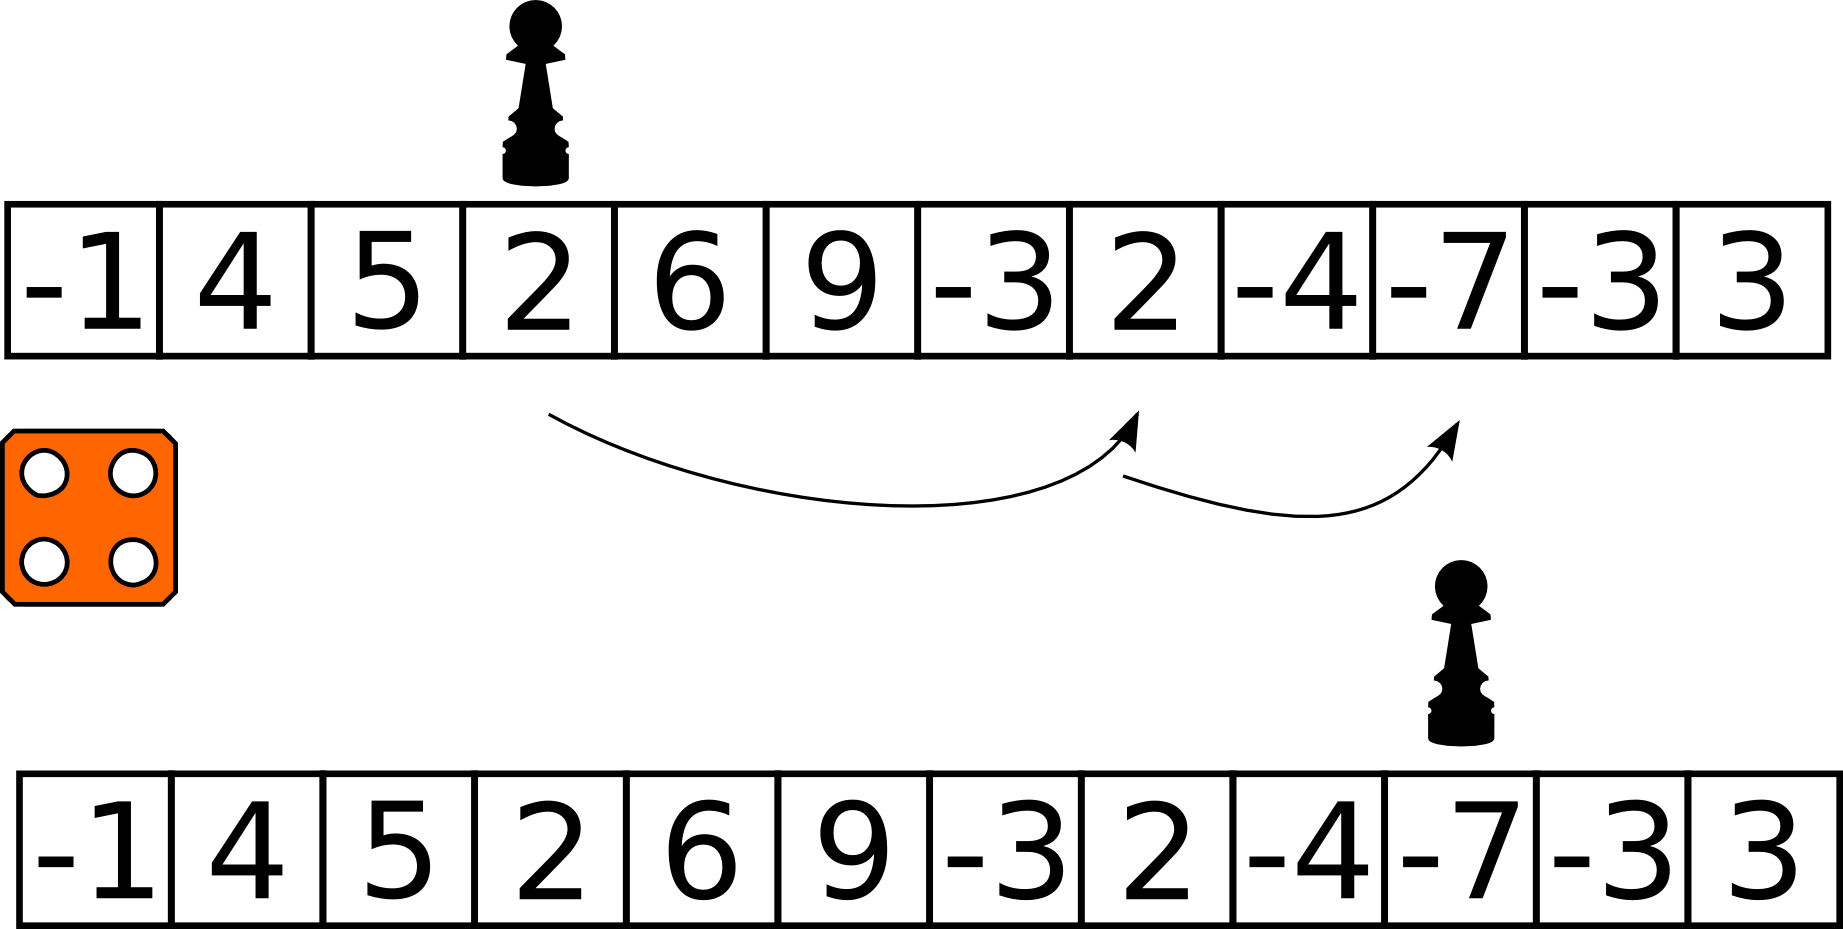
\includegraphics[width=280px]{images/snake-1}
			\end{center}
			
			Le premier joueur à atteindre ou dépasser la dernière case a gagné.
			Nous supposerons que cette dernière case est en position 42. Nous
			supposons également que la première et la dernière case n’ont ni
			échelle ni serpent (valeur nulle).
	
		\subsubsection*{Positions des joueurs}
		
			Les positions des joueurs seront mémorisées dans un tableau
			d’entiers.  Toutes les cases de ce tableau sont initialisées à 0. 
		
			Le plateau de jeu, un tableau d’entiers s’appellera \textbf{chemin}. 
		
			Le tableau d’entiers contenant la position courante des joueurs
			s’appellera \textbf{positionsJoueurs}. 
		
			S’il y a 4 joueurs, le tableau \textit{positionsJoueurs} contient 
			[2,5,1,7] alors~:
			\begin{itemize}
				\item le joueur 0 est en position 2 sur le chemin~;
				\item le joueur 1 est en position 5 sur le chemin~;
				\item le joueur 2 est en position 1 sur le chemin~;
				\item le joueur 3 est en position 7 sur le chemin~;
			\end{itemize}
				
		\subsubsection*{Le premier jour, initialiser le chemin}
		
			Écrivez un algorithme 
			\begin{java}
public static int[] créerChemin(int n)
			\end{java}
			
			Cet algorithme \textit{créerChemin} créera un tableau d’entiers dont
			les valeurs seront des valeurs aléatoires comprises strictement
			entre -10 et 10 (inclus). 
		
			Nous supposons que l’entier $n$ est un naturel strictement supérieur
			à 0.  Vous ne devez pas le vérifier. 
	
		\subsubsection*{Qui est en tête~?}
	
			Écrivez un algorithme 
	
			\begin{java}
public static int enPremièrePosition(int[] positionsJoueurs)
			\end{java}

			Cet algorithme retourne le numéro du joueur en tête de la course. 
			Il recherche donc le maximum dans le tableau passé en
			argument et retourne l’indice de ce maximum. 
	
		\subsubsection*{Jouer un tour de jeu}
	
			Cet algorithme permettra de jouer un tour de jeu pour un joueur
			donné. Jouer un tour de jeu consiste à le faire avancer ou reculer
			(c’est-à-dire changer sa position) du bon nombre de cases. 
	
			\begin{java}
public static void jouer(int[] chemin,
		int[] positionsJoueurs,
		int joueurCourant,
		int valeurDé)
			\end{java}
		
			Cet algorithme fait changer de position le joueur d’indice
			\textit{joueurCourant} de la valeur donnée par le dé
			(\textit{valeurDé}) en respectant les règles du jeu. 
		
			Cet algorithme met donc à jour le tableau \textit{positionsJoueurs}. 
		
			Comme le joueur ne peut se placer sur une case déjà occupée, il peut
			être utile d’écrire un module \texttt{estOccupé} précisant si la
			case est libre ou occupée.  
	
		\end{Exercice}


		\begin{Exercice}{Les algorithmes en maternelle}

		En maternelle, déjà, les enfants font des algorithmes 
		mais il s’agit d’une chose un peu différente.
		On leur propose un collier\footnote{%
			Par exemple, mais ça peut aussi être une chenille,
			un escargot, une simple suite de cases\dots
		}
		dessiné sur une feuille de papier 
		et ils doivent le colorier en répétant un
		\emph{motif} donné\footnote{%
			Ce qu’ils appellent un \emph{algorithme}.
		}, 
		une séquence précise de couleurs.
		
		Par exemple, on donne ce collier 
		 
		\perle{red}-\perle{red}-\perle{green}-\perle{white}-\perle{white}-\perle{white}-\perle{white}-\perle{white}-\perle{white}-\perle{white}\ 
		
		qui est précolorié avec deux perles rouges et une perle verte, c’est le
		motif\footnote{Pour cet exercice, le lecteur est content s'il a la
		version couleurs des notes.}.  
		
		Le résultat attendu est~:
		
		\perle{red}-\perle{red}-\perle{green}-\perle{red}-\perle{red}-\perle{green}-\perle{red}-\perle{red}-\perle{green}-\perle{red}.
		
		Comme on peut le constater sur cet exemple, un motif peut comporter
		plusieurs perles de la même couleur et, en fin de collier, il est
		possible qu’on ne puisse appliquer qu’une partie du motif.
		
		\textbf{Nous allons représenter chaque perle par un caractère
		indiquant sa couleur et un collier comme un tableau de caractères.
		Une perle non coloriée sera indiquée par un point (\Verb_'.'_).}
		
		Par exemple, le collier ci-dessus serait représenté ainsi~:
		
		\begin{center}
		\begin{tabular}{|*{10}{>{\centering\ttfamily\arraybackslash}m{6mm}|}}
		\hline
		'R' & 'R' & 'V' & '.' & '.' & '.' & '.' & '.' & '.' & '.' \\
		\hline
		\end{tabular}
		\end{center}
	
		\subsubsection*{Créer un collier}
		%-----------------------------------------
		
			Écrivez un algorithme \textbf{créerCollier}
			qui reçoit une taille et crée un collier de cette taille
			où toutes les perles sont non coloriées
			(rappel~: une perle non coloriée est représentée par un point).
			
			On suppose que la taille reçue est bien un entier non négatif.
	
		\subsubsection*{Créer un motif}
		%-----------------------------------------
		
			Écrivez un algorithme \textbf{créerMotif}
			qui reçoit un collier dont aucune perle n’est coloriée
			et qui colorie les premières en fonction des indications
			de l’utilisateur.
			
			Concrètement,
			l’utilisateur entre les couleurs des perles
			en spécifiant à chaque fois, après,
			s’il y a encore une perle à colorier.
			Dans notre exemple de la première page,
			l’utilisateur entrerait successivement~:
			'R', vrai, 'R', vrai, 'V', faux. 
			
			L’algorithme doit vérifier que l’utilisateur
			ne demande pas à colorier plus de perles
			qu’il n’y en a dans le collier.
	
		\subsubsection*{Taille du motif}
		%-----------------------------------------
	
			Écrivez un algorithme \textbf{tailleMotif}
			qui reçoit un collier dont seulement les premières perles sont coloriées
			(c’est le motif qu’il faudra suivre)
			et qui donne la taille de ce motif.
			Dans l’exemple de la première page, il faudra retourner la valeur 3.
			Votre algorithme doit générer une erreur si il n’y a pas de motif à suivre.
	
		\subsubsection*{Suivre un motif}
		%-----------------------------------------
		
			Écrivez un algorithme \textbf{colorier}
			qui reçoit un collier dont seulement les premières perles sont coloriées
			(c’est le motif qu’il faut suivre)
			et qui colorie le reste du collier en suivant ce motif.
			
		\subsubsection*{Vérifier un collier}
		%-----------------------------------------
		
			Écrivez un algorithme \textbf{vérifier}
			qui reçoit un collier complètement colorié
			et la taille du motif de départ et qui vérifie
			si le collier respecte ce motif.
		
		\subsubsection*{Trouver le motif}
		%-----------------------------------------
		
			Écrivez un algorithme \textbf{trouverMotif}
			qui reçoit un collier complètement colorié
			et qui détermine la taille du motif.
			C’est la plus petite séquence qui se répète.
			Comme cas extrème, ce pourrait être le collier tout entier.
		
			Aide~: vous avez déjà tout pour que cet exercice soit facile.


		\end{Exercice}


		\chapter{Les fiches}

Vous trouverez ici toutes les fiches
des algorithmes analysés dans ce cours.

\vspace*{-3cm}
\listoffiche

\clearpage%==============================
\begin{Fiche}{Un calcul simple}
%==============================
\label{fiche:calcul-simple}

\Section{Le problème}
Calculer la surface d’un rectangle à partir de sa longueur et sa largeur.
	
\Section{Spécification}

	\textbf{Données} (toutes réelles et non négatives)~:
		\begin{itemize}
			\item la longueur du rectangle~;
			\item la largeur.
		\end{itemize}
		
	\textbf{Résultat}~: un réel représentant la surface du rectangle.

	\begin{center}	
		\flowalgodd{length (real)}{width (real)}{rectangleArea}{real}
	\end{center}

\Section{Exemples}

	\begin{itemize}
	\item \pc{rectangleArea(3, 2)} donne $6$
	\item \pc{rectangleArea(3.5, 1)} donne $3.5$
	\item \pc{rectangleArea(4, 0)} donne $0$
	\end{itemize}

\Section{Solution}

	La surface d’un rectangle est obtenue en multipliant
	la largeur par la longueur.
	\[
		\textrm{surface} = \textrm{longueur} * \textrm{largeur}
	\]

	\begin{langagenaturel}
		surface = longueur * largeur
	\end{langagenaturel}

	\begin{pseudocode}
		\Algo{rectangleArea}{\Par{length, width}{real}}{real}
			\Return length * width
		\EndAlgo
	\end{pseudocode}

	\begin{java}
public static double rectangleArea(double length, double width){
	return length * width;
	\end{java}

\Section{Vérification / tests}

	\begin{center}
		\begin{tabular}{|c|cccc|c|}
		\hline
		\rowcolor{black!40}
		test \no & longueur & largeur & réponse attendue & réponse fournie & {} \\
		\hline 
		1 & 3   & 2 & 6   & 6   & {\color{ForestGreen}$\checkmark$} \\\hline
		2 & 3.5 & 1 & 3.5 & 3.5 & {\color{ForestGreen}$\checkmark$} \\\hline
		3 & 4 & 0 & 0 & 0 & {\color{ForestGreen}$\checkmark$} \\\hline
		\end{tabular}
	\end{center}				

\Section{Quand l’utiliser~?}

	Ce type de solution peut être utilisé à chaque fois
	que la réponse s’obtient par un calcul simple sur les données.
	Si le calcul est plus complexe, 
	il peut être utile de le décomposer pour accroitre la lisibilité
	(cf. fiche \vref{fiche:calcul-complexe}) 
	
\end{Fiche}

\clearpage%================================
\begin{Fiche}{Un calcul complexe}
%================================
\label{fiche:calcul-complexe}

\Section{Problème}

	Calculer la vitesse moyenne (en km/h) d’un véhicule dont on donne la
	distance parcourue (en mètres) et la durée du parcours (en secondes). 

\Section{Spécification}
	
	\textbf{Données} (toutes réelles et non négatives)~:
		\begin{itemize}
		\item la distance parcourue par le véhicule (en m)~;
		\item la durée du parcours (en s).
		\end{itemize}
		
	\textbf{Résultat}~: la vitesse moyenne du véhicule (en km/h).

	\begin{center}
	\flowalgodd{meters (real)}{seconds (real)}{speed}{real}
	\end{center}

\Section{Exemples}

	\begin{itemize}
	\item \pc{speed(100,10)} donne $36$
	\item \pc{speed(10000,3600)} donne $10$
	\end{itemize}

\Section{Solution}

	La vitesse moyenne est liée à la distance et à la durée par la formule~:
	\[
		\textrm{vitesse} = \frac{\textrm{distance}}{\textrm{durée}}
	\]

	\begin{flushright}
	pour autant que les unités soient cohérentes.
	\end{flushright}

	Ainsi pour obtenir une vitesse en km/h, il faut convertir la distance en
	kilomètres et la durée en heures.  Ce qui donne~:

	\begin{langagenaturel}
		convertir la distance reçue en mètres, en km: / 1000\\
		convertir la durée reçue en secondes, en heure: / 3600\\
		la vitesse est la distance / durée
	\end{langagenaturel}
		
	\begin{pseudocode}
		\Algo{speed}{\Par{meters, seconds}{real}}{real}
			\Decl{km, hours}{real}
			\Let km \Gets meters / 1000
			\Let hours \Gets seconds / 3600
			\Return km / hours
		\EndAlgo
	\end{pseudocode}

	\begin{java}
public static double speed(double meters, double seconds){
	double km;
	double hours;
	km = meters / 1000;
	hours = seconds / 3600;
	return km / hours;
}
	\end{java}

\Section{Vérification / tests}

	\begin{center}
		\begin{tabular}{|c|cccc|c|}
		\hline
			\rowcolor{black!40}
		test \no & dist. (m) & durée (s) & rép. attendue 
			& rép. fournie & {} \\
		\hline 
		1 & 100   & 10   & 36 & 36 & {\color{ForestGreen}$\checkmark$} \\\hline
		2 & 10000 & 3600 & 10 & 10 & {\color{ForestGreen}$\checkmark$} \\\hline
		\end{tabular}
	\end{center}								

\Section{Remarque}

Nous n'avons pas tenu compte des cas où la distance serait nulle et dans ce
cas, la vitesse l'est aussi et où la durée est nulle… dans ce cas la vitesse
serait infinie~!


\Section{Quand l’utiliser~?}

	Ce type de solution peut être utilisé à chaque fois que la réponse s’obtient
	par un calcul complexe sur les données qu’il est bon de décomposer pour
	aider à sa lecture.  Si le calcul est plutôt simple, on peut le garder en
	une seule expression (cf. fiche \vref{fiche:calcul-simple}).
	
\end{Fiche}

\clearpage%===================================
\begin{Fiche}{Un nombre pair}
%===================================
\label{fiche:calcul-pair}

\Section{Problème}
Un nombre reçu en paramètre est-il pair\footnote{\textit{Even} en anglais et \textit{odd} pour impair.}~?

\Section{Spécification}

	\textbf{Données}~: le nombre entier dont on veut savoir si il est pair.
		
	\textbf{Résultat}~: un booléen à \textit{vrai} si le \textit{nombre} est pair et \textit{faux} sinon.

	\begin{center}	
		\flowalgod{number (integer)}{isEven}{boolean}
	\end{center}

\Section{Exemples}

	\begin{itemize}
	\item \pc{isEven(16)} donne $vrai$
	\item \pc{isEven(15)} donne $faux$
	\item \pc{isEven(0)} donne $vrai$
	\end{itemize}
	
\Section{Solution}

	Un nombre est pair si il est multiple de 2. 
	C’est-à-dire si le reste de sa division par 2 vaut 0.

	\begin{langagenaturel}
		n est pair si n modulo 2 = 0
	\end{langagenaturel}

	\begin{pseudocode}
		\Algo{isEven}{\Par{number}{integer}}{boolean}
			\Return number MOD 2 == 0
		\EndAlgo
	\end{pseudocode}

	\begin{java}
public static boolean isEven(int n){
	return n%2 == 0;
}
	\end{java}

	\paragraph{Remarque} C'est mieux de respecter les bonnes pratiques
	d'écriture et d'écrire directement un \pc{return} sans \pc{if} dans ce cas.
	Voir annexe \vref{B-ass-bool}.

\Section{Vérification / tests}

	\begin{center}
		\begin{tabular}{|c|ccc|c|}
		\hline
			\rowcolor{black!40}
		test \no & n & rép. attendue & rép. fournie & {} \\
		\hline 
		1 & 16   & true   & true & {\color{ForestGreen}$\checkmark$} \\\hline
		2 & 15   & false   & false & {\color{ForestGreen}$\checkmark$} \\\hline
		3 & 0   & true   & true & {\color{ForestGreen}$\checkmark$} \\\hline
		\end{tabular}
	\end{center}								

	
\Section{Quand l’utiliser~?}

	À chaque fois qu’un résultat booléen dépend d’un calcul simple.
	Si le calcul est plus compliqué, on peut le décomposer comme
	indiqué dans la fiche \vref{fiche:calcul-complexe}.
	
	On peut également s’inspirer de cette solution
	quand il faut donner sa valeur à une variable booléenne.
		
\end{Fiche}
		
\clearpage%======================================
\begin{Fiche}{Maximum de deux nombres}
%======================================
\label{fiche:max2nb}

\Section{Problème}
	Quel est le maximum de deux nombres~?

\Section{Analyse}

	Voilà un classique de l’algorithmique.  Attention~! On ne veut pas savoir
	\emph{lequel} est le plus grand mais juste la valeur.  Il n’y a donc pas
	d’ambigüité si les deux nombres sont égaux.

	\textbf{Données}~: deux nombres réels.
		
	\textbf{Résultat}~: un réel contenant la plus grande des deux valeurs données.

	\begin{center}	
		\flowalgodd{nb1 (real)}{nb2 (real)}{max2}{real}
	\end{center}

\Section{Exemples}

	\vspace*{-3mm}
	\begin{multicols}{3}
		\begin{itemize}
		\item \pc{max2(-3, 4)} donne $4$
		\item \pc{max2(7, 4)} donne $7$
		\item \pc{max2(4, 4)} donne $4$
		\end{itemize}
	\end{multicols}
	\vspace*{-6mm}
	
\Section{Solution}

	\begin{pseudocode}
	\Algo{max2}{\Par{nb1}{real}, \Par{nb2}{real}}{real}
		\Decl{max}{real}
		\If{nb1 > nb2}
			\Let max \Gets nb1
		\Else
			\Let max \Gets nb2
		\EndIf
		\Return max
	\EndAlgo
	\end{pseudocode}

	Attention à éviter les mauvaises écritures 
	expliquées à l’annexe \vref{B-ass-val}.

	
\Section{Quand l’utiliser~?}

	Cet algorithme peut bien sûr être facilement adapté à la recherche du
	minimum.
		
\end{Fiche}
		
\clearpage%================================
\begin{Fiche}{Passage d’un tableau en paramètre}
%================================
\label{fiche:tab-passage-param}

\Section{Problème}

	Le type \emph{tableau} étant un type à part entière, il est tout-à-fait
	éligible comme type pour les paramètres et la valeur de retour d’un
	algorithme.

\Section{Passer un tableau en paramètre}
		\begin{itemize}
			\item \In : 
				indique que l’algorithme va consulter les valeurs du tableau
				reçu en paramètre.  Les éléments doivent donc avoir été
				initialisés avant d’appeler l’algorithme. Exemple~:
			
				\begin{pseudocode}
					\LComment{Affiche les éléments d’un tableau de n entiers}
					\Algo{display}{\Par{is\In}{\Array{}{integer}}}{} 
						\For{i}{0}{is.length - 1}
							\Write is[i]
						\EndFor
					\EndAlgo 
					
					\LComment{Utilisation possible}
					\Decl{myIntegers}{\Array{10}{entiers}}
					\Let myIntegers \Gets \{2,3,5,7,11,13,17,19,23,29\}
					\Stmt afficher(myIntegers)
				\end{pseudocode}
				
				\textbf{Rappel} C'est  le passage de paramètre par défaut si
				aucune flèche n’est indiquée.
				
			\item \In\Out :
				indique que l’algorithme va consulter/modifier les valeurs 
				du tableau reçu en paramètre. Exemple~:
			
				\begin{pseudocode}
					\LComment{Inverse le signe des éléments d'un tableau de 
						n entiers}
					\Algo{oppositeValues}{\Par{is\In\Out}{\Array{}{integer}}}{} 
						\For{i}{0}{is.length - 1}
							\Let is[i] \Gets -is[i]
						\EndFor
					\EndAlgo 
		
					\LComment{Utilisation possible}
					\Decl{myIntegers}{\Array{5}{entiers}}
					\Let myIntegers \Gets \{2,-3,5,-7,11\}
					\Stmt oppositeValues(myIntegers)
				\end{pseudocode}

			\end{itemize}

			\paragraph{Rappel Java~:} Un tableau Java étant un type référence,
			c'est toujours la valeur de la référence qui est passée en
			paramètre.  En ce sens, un passage en entrée ou en entrée / sortie
			est identique en Java et le tableau doit toujours exister
			c'est-à-dire avoir été créé au préalable. 

		\Section{Retourner un tableau}
		%---------------------------------
			
			Comme pour n’importe quel autre type, un algorithme peut retourner
			un tableau.  Ce sera à lui de le déclarer et de lui donner des
			valeurs.

			\textbf{Exemple~:}
			\begin{pseudocode}
				\LComment Crée un tableau d’entiers de taille n, 
					l’initialise à 0 et le retourne.
				\Algo{create}{n : integer}{\Array{n}{integer}}
					\Decl{is}{\Array{n}{integer}}
					\For{i}{0}{n-1}
						\Let is[i] \Gets 0
					\EndFor
					\Return is
				\EndAlgo
				\Empty
				\LComment{Utilisation possible}
				\Algo{test}{}{}
					\Decl{myIntegers}{\Array{}{integer}}
					\Let myIntegers \Gets create(20)
					\Stmt display(myIntegers)
				\EndAlgo
			\end{pseudocode}
	
\end{Fiche}
		
\clearpage%================================
\begin{Fiche}{Parcours complet d’un tableau}
%================================
\label{fiche:tab-parcours-complet}

\Section{Problème} 

Parcours complet d'un tableau pour afficher tous les éléments. Par exemple un
tableau de \pc{double}.

\Section{Spécification}
	
	\begin{itemize}
	\item \textbf{Données}~: le tableau à afficher
	\item \textbf{Résultat}~: aucun.
	\item \textbf{Affiche} : les éléments du tableau, dans l'ordre.
	\end{itemize}

\Section{Solution}

	Puisqu’on parcourt tout le tableau, on peut utiliser une boucle \emph{pour}
	(\pc{for}).
	
	\begin{pseudocode}
		\Algo{display}{\Par{ds}{\Array{}{real}}}{}
			\For{i}{0}{ds.length - 1}
				\Write ds[i]
			\EndFor
		\EndAlgo
	\end{pseudocode}

	\begin{java}
// Utilisation d'un for
public static void display (double[] ds){
	for (int i=0; i < ds.length; i++){
		System.out.println(ds[i]);
	}
}
	\end{java}

	Si l'on n'a pas besoin de modifier la valeur dans le tableau et que l'on
	veut simplement utiliser la valeur — dans ce cas, pour l'afficher — on peut
	utiliser une boucle \textit{enhanced for}\index{foreach} comme suit~:

	\begin{java}
// Utilisation d'un enhanced for (foreach)
public static void display (double[] ds){
	for (double d: ds){
		System.out.println(d);
	}
}
	\end{java}

\Section{Quand l’utiliser~?}

	Ce type de solution peut être utilisé à chaque fois qu’il est nécessaire
	d'examiner \textbf{tous} les éléments d’un tableau, quel que soit le
	traitement voulu~: les afficher, les sommer, les comparer\dots

	L'\textit{enhanced for} ne permet pas de modifier les éléments du tableau. 
	
	
\end{Fiche}
		
\clearpage%================================
\begin{Fiche}{Parcours partiel d’un tableau}
%================================
\label{fiche:tab-parcours-partiel}

\Section{Problème}

	Parcours partiel d'un tableau pour rechercher un zéro. Par exemple avec un
	tableau de \pc{double}.

\Section{Spécification}
	
	\textbf{Données}~: le tableau à tester
		
	\textbf{Résultat}~: 
		un booléen à vrai si il existe une valeur nulle dans le tableau.
	
	\begin{center}	
		\flowalgod{ds (tableau de pseudo-réels)}{containsNulValue}{booléen}
	\end{center}

\Section{Solution}

	Contrairement au parcours complet (cf. fiche
	\vref{fiche:tab-parcours-complet}) nous allons utiliser un \emph{tant que}
	(\pc{while}) car nous voulons arrêter l'algorithme dès que la valeur
	cherchée est trouvée.
	
	Il existe essentiellement deux solutions, avec ou sans variable booléenne.
	En général, la première solution [A] sera plus claire si le test est court.

	\subsubsection*{[A] Sans variable booléenne}
	
		\begin{pseudocode}
			\Algo{containsNulValue}{\Par{ds}{\Array{}{double}}}{boolean}
				\Decl{i}{integer}
				\Let i \Gets 0
				\While{i < ds.length AND ds[i] $\neq$ 0}
					\Let i \Gets i + 1
				\EndWhile
				\Return i < n \RComment Si i<n -> arrêt prématuré 
					\Let\RComment c-à-d que l'on a trouvé un 0.
			\EndAlgo
		\end{pseudocode}

		\begin{java}
public static boolean containsNulValue(double[] ds){
	int i = 0;
	while (i < ds.length && ds[i] != 0){
		i++;
	}
	/* Si i < n c'est un arrêt prémature et c'est que l'on a trouvé */
	return i < n
}
		\end{java}
	
		Il faut être attentif à \textbf{ne pas inverser} les deux parties du
		test sous peine de générer une erreur parce que l'on essaie d'accéder
		à un élément hors du tableau.  Il faut absolument vérifier que l’indice
		est bon avant de tester la valeur à cet indice. Se ce n'est pas clair,
		revoir la notion d'évaluation paresseuse (court-circuit). Voir
		\vref{court-circuit}.
		

	\subsubsection*{[B] Avec variable booléenne}

		\begin{pseudocode}
			\Algo{containsNulValue}{\Par{is}{\Array{}{integer}}}{boolean}
				\Decl{i}{integer}
				\Decl{isZero}{boolean}
				\Let isZero \Gets false
				\Let i \Gets 0
				\While{i < is.length AND NON isZero}
					\Let isZero \Gets is[i] ==  0
					\Let i \Gets i + 1
				\EndWhile
				\Return isZero
			\EndAlgo
		\end{pseudocode}

		\begin{java}
public static boolean containsNulValue(double[] ds){
	int i = 0;
	boolean isZero = false;
	while (i < ds.length && !isZero){
		isZero = ds[i] == 0;
		i++;
	}
	return isZero;
}
		\end{java}

		Au sortir de la boucle, l’indice \pc{i} ne désigne pas l’élément qui
		nous a permis d’arrêter mais le suivant.  Si nécessaire, on peut
		remplacer l’intérieur de la boucle par~:

		\begin{java}
if (ds[i] == 0){
	isZero = true;
} else {
	i++;
}
		\end{java}
		
		Dans notre exemple, nous cherchons un élément particulier (un 0).  Dans
		le cas où l'on vérifie si tous les éléments possèdent une certaine
		propriété (être positifs par exemple), nous veillerons à adapter le nom
		du booléen et son utilisation (par exemple un booléen appelé
		\pc{areAllPositives}, initialisé à \pc{true} avec un \pc{\dots AND
		areAllPositives} dans le test.

		Dans tous les cas, faites attention à ne pas acdéder à l'élément
		—~utiliser \pc{ds[i]}~— si vous n’êtes pas sûr de l'indice \pc{i}.
		C’est particulièrement vrai après la boucle.

		\paragraph{Remarque} C'est mieux de respecter les bonnes pratiques
		d'écriture et d'écrire directement un \pc{return} sans \pc{if} dans ce
		cas.  Voir annexe \vref{B-for-break}.
		
					
\Section{Quand l’utiliser~?}

	Ce type de solution peut être utilisé pour tout parcours d'un tableau où un
	arrêt prématuré est possible en se posant les questions suivantes~:

	\begin{itemize}
	\item Est-ce que tous les éléments sont positifs~?
	\item Est-ce que les élément sont triés~?
	\item Est-ce qu’un élément précis est présent~?
	\item \dots
	\end{itemize}
	
\end{Fiche}
		
\clearpage%================================
\begin{Fiche}{Maximum dans un tableau}
%================================
\label{fiche:tab-max}

\Section{Problème}
	Trouver la valeur maximale dans un tableau d’entiers.

\Section{Spécification}
	
	\textbf{Données}~: le tableau à analyser

	\textbf{Résultat}~: la valeur du maximum

\Section{Solution}

	Il faut veiller à initialiser le maximum avec la première valeur du tableau
	pour parcourir le reste du tableau à la recherche d’une valeur plus grande.
	
	\begin{pseudocode}
		\Algo{max}{\Par{is}{\Array{}{integer}}}{integer}
			\Decl{max}{integer}
			\Let max \Gets is[0]
			\For{i}{1}{is.length - 1}
				\If{is[i] > max}
					\Let max \Gets is[i]
				\EndIf
			\EndFor
			\Return max
		\EndAlgo
	\end{pseudocode}

\Section{Variante}

	Si c'est la position et non la valeur qui nous intéresse, une solution 
	serait~:

	\begin{pseudocode}
		\Algo{max}{\Par{is}{\Array{}{integer}}}{integer}
			\Decl{maxIndex}{integer}
			\Let maxIndex \Gets 0
			\For{i}{1}{is.length - 1}
				\If{is[i]>is[maxIndex]}
					\Let maxIndex \Gets i
				\EndIf
			\EndFor
			\Return maxIndex
		\EndAlgo
	\end{pseudocode}
	
	
\end{Fiche}
		
\clearpage%================================
\begin{Fiche}{Tableau non trié}
%================================
\label{fiche:tab-recherche-non-triee}

\Section{Problème}
	
	Rechercher, ajouter, supprimer des données non triées dans un tableau
	d’entiers non triés.

\Section{Rechercher}

	Retourner l'indice d'une donnée trouvée dans un tableau non trié ou -1 si
	elle n'est pas trouvée. 

	Nous supposons que le tableau n'est pas rempli, l'algorithme recevra donc 
	une valeur représentant le nombre d'éléments du tableau. Cette valeur est
	inférieure à la taille du tableau bien sûr. 
	
	\textbf{Données}~: le tableau à analyser, le nombre d'éléments dans ce
	tableau (taille logique), la valeur à rechercher
		
	\textbf{Résultat}~: la position de l'élément si il est dans le tableau et -1
	sinon
	
		\begin{pseudocode}
			\LComment{Vérifie si un nombre est dans un tableau 
			et donne sa position (-1 sinon)}
			\Algo{indexValue}{\Par{is\In}{\Array{}{integers}}, 
					\\\hfill\Par{nbValues\In}{integer}, 
					\Par{value\In}{integer}}{integer}
				\Decl{i}{integer}
				\Let i \Gets 0
				\While{i < nbValues AND is[i] $\ne$ value}
					\Let i \Gets i + 1
				\EndWhile
				\If{i < nbValues}
					\Return i
				\Else
					\Return -1
				\EndIf
			\EndAlgo
		\end{pseudocode}

\Section{Ajouter}
	Ajouter une donnée non encore présente dans le tableau de données non triées
	
	\textbf{Données}~: le tableau à modifier, le nombre d'éléments dans ce
	tableau, la valeur à ajouter
		
	\textbf{Résultat}~: le tableau reçu est modifié en lui ajoutant la valeur si
	elle n'y était pas déjà
	
		\begin{pseudocode}
			\LComment{Ajoute un nombre non encore présente dans le isleau.}
			\Algo{add}{\Par{is\In\Out}{\Array{}{integer}}, 
				\\\hfill\Par{nValues\In\Out}{integer}, \Par{value\In}{integer}}{}
				\If{nValues $<$ is.length 
						AND indexValue(is, nValues, value) $\ne$ -1}
					\Let is[nValues] \Gets value
					\Let nValues \Gets nValues + 1
				\EndIf
			\EndAlgo
		\end{pseudocode}

		\paragraph{Remarque} Si l'algorithme précédent se traduit immédiatement
		en langage Java, ce n'est pas le cas de celui-ci. Pourquoi ? 
	
		Le passage de paramètre se faisant par valeur (cfr. chapitre
		\ref{chap:insertion-recherche} p.~\pageref{chap:insertion-recherche}),
		la taille logique du tableau doit être retournée et maintenue à jour par
		le code appelant. En langage Java, cet algorithme aurait l'allure
		suivante~:

		\begin{java}
public static int add(int[] is, int nValues, int value){
	if (nValues < is.length() 
			&& indexValue(is, nValues, value) != -1){
		is[nValues] = value;
		nValues = nValues + 1;
	}
	return nValues;
}
		\end{java}


\Section{Supprimer}
	Supprimer une donnée d'un tableau de données non triées
	
	\textbf{Données}~: le tableau à modifier, le nombre d'éléments dans ce
	tableau, la valeur à supprimer
		
	\textbf{Résultat}~: le tableau reçu est modifié en lui supprimant la valeur
		
		\begin{pseudocode}
			\LComment{Supprime un nombre donné dans le tableau.}
			\Algo{delete}{
				\Par{is\In\Out}{\Array{n}{integer}}, 
				\\\hfill\Par{nValues\In\Out}{integer}, 
				\Par{value\In}{integer}
			}{}
				\Decl{index}{integer}
				\Let index \Gets indexValue(is, nValues, value)
				\If{index $\ne$ -1}
					\Let is[index] \Gets is[nValues-1]
					\Let nValues \Gets nValues - 1
				\EndIf			
			\EndAlgo
		\end{pseudocode}

%\Section{Variante}


	
\end{Fiche}

\clearpage%================================
\begin{Fiche}{Tableau trié}
%================================
\label{fiche:tab-recherche-triee}

\Section{Problème}
	
	Rechercher, ajouter, supprimer des données triées dans un tableau trié. Par
	exemple dans un tableau d'entiers. 

\Section{Rechercher}

\SubSection{Spécification}

	Rechercher la position où a été trouvé l’élément ou la position où il aurait
	dû être.
	
	\textbf{Données}~: le tableau à analyser, le nombre d'éléments dans ce
	tableau, la valeur à rechercher
		
	\textbf{Résultat}~: la position où a été trouvée la valeur ou la position où
	elle aurait dû être

	\SubSection{Solution}

	L'algorithme retourne la position où a été trouvée la valeur \textbf{ou}
	celle où elle devrait être. En parcourant le tableau, il suffit de
	s'arrêter dès que l'élément du tableau est plus grand ou égal à la valeur
	recherchée. 

		\begin{pseudocode}
				\LComment{Recherche un élément.}
				\LComment{- index~: indique la position où a été trouvée la valeur}
				\LComment{ou la position où elle aurait dû être}
				\Algo{findIndex}{
						\Par{is\In}{\Array{}{integer}}, 
						\Par{nValues\In}{integer}, 
						\\\hfill\Par{value\In}{integer},
						}{index integer}
					\Decl{index}{integer} \Gets 0
					\While{index < nValues AND is[index] < value}
						\Let index \Gets index + 1
					\EndWhile
					\Return index
				\EndAlgo
		\end{pseudocode}

		\begin{java}
public static int findIndex(int[] is, int nValues, int value){
	int index = 0;
	while (index < nValues && is[index] < value){
		index++;
	}
	return index;
}
		\end{java}


\Section{Ajouter}

	\SubSection{Spécification}
	
	Ajouter une donnée non encore présente dans le tableau de données triées.
	
	\textbf{Données}~: le tableau à modifier, le nombre d'éléments dans ce
	tableau, la valeur à ajouter
		
	\textbf{Résultat}~: le tableau reçu est modifié en lui ajoutant la valeur si
	elle n'y était pas déjà

	\SubSection{Solution}

	Pour faire un ajout sans doublon dans un tableau triée, il faut~:

	\begin{enumerate}
		\item vérifier que la valeur n'est pas déjà présente\,;
		\item rechercher l'endroit ou elle devrait être placée\,;
		\item déplace les valeurs plus grande d'une position vers la droite\,;
		\item insère la valeur à sa place. 
	\end{enumerate}

	En décomposant le problème, voici une solution~:

	\begin{pseudocode}
		\LComment{Ajouter un nombre donné.}
		\Algo{add}{
				\Par{is\In\Out}{\Array{}{integer}}, 
				\Par{nValues\In}{integer}, 
				\\\hfill\Par{value\In}{integer}
				}{integer}
			\Decl{index}{integer}
			\Decl{isFound}{boolean}
			\If{verify(is, nValues, value) == -1}
				\Stmt index \Gets findIndex(is, nValues, value)
				\Stmt shiftRight(is, index, nValues)
				\Let is[index] \Gets value
				\Let nValues \Gets nValues + 1
			\EndIf
			\Return nValues
		\EndAlgo
		\LComment{Vérifie si un nombre est dans un tableau d'entiers trié}
		\LComment{et donne sa position (-1 si non présent)}
		\Algo{verify}{
			\Par{is\In}{\Array{}{integers}}, 
			\Par{nValues\In}{integer}, 
			\\\hfill
			\Par{value\In}{integer}
		}{integer}
			\Decl{index}{integer}
			\Decl{isFound}{boolean}
			\Stmt index \Gets findIndex( is, nValues, value)
			\If{is[index] == value}
				\Return index
			\Else
				\Return -1
			\EndIf
		\EndAlgo
		\LComment{Décale d’une position à droite les éléments}
		\LComment{entre la position début et fin}
		\Algo{shiftRight}{
				\Par{is\In\Out}{\Array{}{integer}}, 
				\Par{begin\In}{integer}, 
				\Par{end\In}{integer}
				}{}
			\For[-1]{i}{end}{begin}
				\Let is[i+1] \Gets is[i]
			\EndFor
		\EndAlgo
	\end{pseudocode}

	\begin{java}
/**
 * Ajoute un nombre s'il n'est pas présent.
 * 
 * @param is le tableau d'éléments
 * @param nValues le nombre d'éléments du tableau (taille logique)
 * @param value la valeur à insérer
 */
public static int add(int[] is, int nValues, int value){
	int index;
	if (verify(is, nValues, value) == -1){
		index = findIndex(is, nValues, value);
		shiftRight(is, index, nValues);
		is[index] = value;
		nValues++;
	}
	return nValues;
}

/**
 * Vérifie si la valeur est dans le tableau. 
 *
 * @param is le tableau d'éléments
 * @param nValues le nombre d'éléments du tableau (taille logique)
 * @param value la valeur à insérer
 */
public static int verify(int[] is, int nValues, int value){
	int index = findIndex(is, nValues, value);
	if (is[index] == value) {
		return index;
	} else {
		return -1;
	}
}

/**
 * Décale d'une position vers la droite les éléments 
 * entre position début et fin. 
 * 
 * @param is le tableau d'éléments
 * @param begin la position de début
 * @pasam end la position de fin
 */
public static void shiftRight(int[] is, int begin, int end){
	for (int i = end; i >= begin; i--){
		is[i+1] = is[i];
	}
}
	\end{java}

\clearpage
\Section{Supprimer}

	\SubSection{Spécification}

	Supprimer une donnée d'un tableau de données triées.
	
	\textbf{Données}~: le tableau à modifier, le nombre d'éléments dans ce
	tableau, la valeur à supprimer
		
	\textbf{Résultat}~: le tableau reçu est modifié en lui supprimant la valeur
		
	\SubSection{Solution}

	Pour supprimer un élément, dès dès lors qu'il est trouvé, il suffit de décaler tous les élémens à sa droite vers la gauche et adapter la taille logique. 

	\begin{pseudocode}
		\LComment{supprimer l'élément donné}
		\Algo{delete}{
			\Par{is\In\Out}{\Array{}{integer}}, 
			\Par{nValues\In\Out}{integer}, 
			\\\hfill\Par{value\In}{integer}
		}{integer}
			\Decl{index}{integer}
			\Decl{isFound}{boolean}
			\If{verify(is, nValues, value) $\neq$ -1}
				\Stmt index \Gets findIndex(is, nValues, value)
				\Stmt shiftLeft(is, index + 1, nValues)
				\Let nValues \Gets nValues - 1	
			\EndIf
			\Return nValues
		\EndAlgo
		\Empty
		\LComment{Décale d’une position à gauche les éléments }
		\LComment{entre la position début et fin}
		\Algo{shiftLeft}{
			\Par{tab\In\Out}{\Array{}{integers}}, 
			\Par{begin\In}{integer}, 
			\Par{end\In}{integer}
		}{}
			\For{i}{begin}{end}
				\Let is[i-1] \Gets is[i]
			\EndFor
		\EndAlgo
	\end{pseudocode}

	\begin{java}
public static int delete(int[] is, int nValues, int value){
	int index;
	if (verify(is, nValues, value) != -1){
		index = findIndex(is, nValues, value);
		shiftLeft(is, index+1, nValues);
		nValues = nValues - 1;
	}
	return nValues;
}

public static void shiftLeft(int[] is, int begin, int end){
	for (int i=begin; i <= end; i++){
		is[i-1] = is[i];
	}
}
	\end{java}

\end{Fiche}

\clearpage%================================
\begin{Fiche}{Recherche dichotomique}
%================================
\label{fiche:dicho}

\Section{Problème}

	Trouver rapidement la position d’une valeur donnée dans un tableau
	\textbf{trié} d’entiers.  Si la valeur n’est pas présente, on donnera la
	position où elle aurait du se trouver.

	Voir Section~\vref{chap:recherche-dichotomique}.

\Section{Spécification}
	
	\textbf{Données}~: le tableau à analyser et la valeur recherchée
		
	\textbf{Résultat}~: un booléen indiquant si la valeur a été trouvée et un
	entier indiquant soit la position où la valeur a été trouvée soit la
	position où elle aurait du être.

\Section{Solution}

		L’algorithme rapide que nous avons vu est la recherche
		dichotomique.

		\inputjava{algo-standards/binarySearch.java}

		\clearpage
		Dans le cas d'un langage permettant d'autres passages de paramètres que
		le passage par valeur (cfr.~Section~\vref{paramètres}), nous pourrions
		écrire un algorithme~:

		\begin{itemize}
			
			\item qui retourne un booléen présisant si la valeur est trouvée
				et\,;

			\item qui donne la position à laquelle se trouve la valeur ou la
				position à laquelle elle devrait se trouver ce qui serait
				pratique en cas d'insertion. 

		\end{itemize}

		Un tel algorithme aurait cette allure~:
	
		\begin{pseudocode}
			\Algo{dichotomousSearch}{
					\\\hfill
					\Par{myArray\In}{\Array{}{integers}}, 
					\Par{value\In}{integer}, 
					\Par{pos\InOut}{integer}
					}{boolean}
				\Decl{rightIndex, leftIndex, medianIndex}{integer}
				\Decl{candidate}{integer}
				\Decl{isFound}{boolean}
				\Empty
				\Let leftIndex \Gets 0
				\Let rightIndex \Gets myArray.length - 1
				\Let isFound \Gets false
				\Empty
				\While{NON isFound AND leftIndex {${\leq}$} rightIndex}
					\Let medianIndex \Gets (leftIndex + rightIndex) DIV 2
					\Let candidate \Gets myArray[medianIndex]
					\If{candidate == value} 
						\Let isFound \Gets vrai
					\ElsIf{candidate < value}
						\Let leftIndex \Gets medianIndex + 1
						\RComment on garde la partie droite
					\Else
						\Let rightIndex \Gets medianIndex – 1
						\RComment on garde la partie gauche
					\EndIf
				\EndWhile
				\Empty
				\If{isFound}
					\Let pos \Gets medianIndex
				\Else
					\Let pos \Gets leftIndex
					\RComment dans le cas où la valeur n’est pas trouvée,
					\Empty 
					\RComment on vérifiera que leftIndex donne la valeur 
					où elle pourrait être insérée.
				\EndIf
				\Empty
				\Return isFound
			\EndAlgo
		\end{pseudocode}
\end{Fiche}
		
\clearpage%================================
\begin{Fiche}{Tri d’un tableau}
%================================
\label{fiche:tri}

\noindent Trier un tableau d’entiers par ordre croissant. Les algorithmes de tri sont présentés aux sections \vrefrange{chap:tri-insertion}{chap:tri-bubble}.

\Section{Spécification}
	
	\textbf{Données}~: le tableau non trié, à trier.
		
	\textbf{Résultat}~: ce même tableau trié.

\Section{Solution}

\subsection*{Le tri par insertion}
		
	\begin{pseudocode}
		\LComment Trie le tableau reçu en paramètre (via un tri par insertion).
		\Algo{insertionSort}{\Par{myArray\InOut}{\Array{}{integers}}}{}
			\Decl{i, j, value}{integers}
			\For{i}{1}{myArray.length - 1}
				\Let value \Gets myArray[i]
				\LComment recherche de l’endroit où insérer value dans le 
				\LComment sous-tableau trié et décalage simultané des éléments
				\Let j \Gets i - 1
				\While{j ${\geq}$ 0 AND value < myArray[j]}
					\Let myArray[j+1] \Gets myArray[j]
					\Let j \Gets j – 1
				\EndWhile
				\Let myArray[j+1] \Gets value
			\EndFor
		\EndAlgo
	\end{pseudocode}

        \inputjava{algo-standards/insertionSort.java}


	
\subsection*{Le tri par sélection des minima successifs}
		
	\begin{pseudocode}
		\LComment Trie le tableau reçu en paramètre 
		(via un tri par sélection des minima successifs).
		\Algo{selectionSort}{\Par{myArray\InOut}{\Array{}{integers}}}{}
			\Decl{i, minIndex}{integer}
			\For{i}{0}{myArray.length – 2}
			\RComment i correspond à l’étape 
			\RComment de l’algorithme
				\Let minIndex \Gets searchMinIndex( myArray, i, 
					myArray.length - 1 )
				\Stmt swap( myArray[i], myArray[minIndex] )
			\EndFor
		\EndAlgo

		\Empty
		\LComment Retourne l’indice du minimum entre les indices début 
		et fin du tableau reçu.
		\Algo{searchMinIndex}{
			\Par{myArray\In}{\Array{}{integers}}, 
			\\\hfill\Par{début\In, fin\In}{integers}}{integer}
			\Decl{minIndex, i}{integers}
			\Let minIndex \Gets début
			\For{i}{début+1}{fin}
				\If{myArray[i] < myArray[minIndex]}
					\Let minIndex \Gets i
				\EndIf
			\EndFor
			\Return minIndex
		\EndAlgo

		\Empty
		\LComment {Échange le contenu de 2 variables.}
		\Algo{swap}{\Par{a\InOut, b\InOut}{integers}}{}
			\Decl{aux}{integer}
			\Let aux \Gets a
			\Let a \Gets b
			\Let b \Gets aux
		\EndAlgo
	\end{pseudocode}

	\inputjava{algo-standards/selectionSort.java}


	

\subsection*{Le tri bulle}

	\begin{pseudocode}
	\LComment Trie le tableau reçu en paramètre (via un tri bulle).
		\Algo{bubbleSort}{\Par{myArray\InOut}{\Array{}{integers}}}{}
			\Decl{burstIndex, bubbleIndex}{integers}
			\For{burstIndex}{0}{myArray.length - 2}
				\For[-1]{bubbleIndex}{myArray.length – 2}{burstIndex}
					\If{myArray[bubbleIndex] > myArray[bubbleIndex + 1]}
                                        	\LComment voir algorithme précédent
						\Stmt swap( myArray[bubbleIndex], myArray[bubbleIndex + 1] )
					\EndIf
				\EndFor
			\EndFor
		\EndAlgo
	\end{pseudocode}

        \inputjava{algo-standards/bubbleSort.java}

\end{Fiche}
		

		\chapter{Bonnes pratiques}
\label{bonnespratiques}

	Ce chapitre recense quelques bonnes pratiques d'écriture d'algorithme et de
	code. Il montre également des manières d'écrire du code peu lisibles et donc
	à éviter, voire à proscrire. 
	
	Les bonnes pratiques d'écriture ont également un aspect culturel et
	dépendant d'un langage. En effet, certaines communautés de programmeurs
	habitués à un langage adoptent des styles de programmation qui ne sont pas
	partagés par d'autres programmeurs, habitués à un autre langage. Nous
	présentons ici des bonnes pratiques d'algorithmique générale et des bonnes
	pratiques liées au langage Java. 

	\begin{quote}
		
		{\Large «}~Lorsque je code en langage Java, je respecte les conventions
		du langage Java. 
		Lorsque je code en langage C++, je respecte les
		conventions du langage C++. 

		Lorsque je contribue à un projet, je respecte les conventions du
		langage et celles proposées par l'équipe en charge du projet.~{\Large»}

	\end{quote}

\minitoc


%===================================================
\section{Bonnes pratiques générales}
%===================================================

	Certaines conventions d'écriture, sont communes à tous les langages. Citons
	par exemple~:

	\begin{itemize}

		\item préferer des lignes de longueur maximale de 80 caractères. Ceci
			facilite la lecture\,;
		
		\item couper les lignes qui seront trop longues en suivant ces règles\,;

			\begin{itemize}
				
				\item couper après une virqule\,;
				\item couper avant un opérateur\,;

				\item préférer les coupures de haut niveau de priorité aux
					coupures de priorité faible\,;

				\item aligner la nouvelle ligne avec le début de l'expression
					se trouvant à la ligne précédente.

			\end{itemize}
			
	\end{itemize}

	Nous vous invitons à consulter les conventions d'écriture du code en Java
	—~même si le document est vieux~— ceci afin d'écrire un code plus lisible.
	Voir \cite{java-codeconv}

%===================================================
\section{Tester un booléen}
%===================================================

	Lorsqu’il s’agit de comparer deux nombres dans la condition d’un \K{if},
	nous écrivons assez naturellement~: \pc{\K{if} (nb1<nb2)} et il ne vous
	viendrait pas à l’idée d’écrire~: \pc{\K{if} (nb1<nb2 == true)}.
	
	\bigskip
		
	Avec un booléen, nous allons également éviter d'écrire \pc{== true} ou
	\pc{== false}.  Par exemple, pour exécuter un traitement si la variable
	\pc{isAdult} est vraie, certaines personnes programmeuses débutantes écrivent
	ceci~:
	
	\marginicon{dont}
	\begin{java}
		if (isAdult == true){
			// ...
		}
	\end{java}

	Cette écriture est correcte mais inutilement lourde.  La variable étant déjà
	un booléen qui vaut vrai ou faux, il suffit d’écrire~:

	\begin{java}
if (isAdult){
	// ...
}
	\end{java}

	C'est une bonne pratique d'utiliser cette deuxième écriture. 
	
	De même, si le test doit être vrai quand la variable booléenne est fausse,
	il suffit d’écrire~: 
	
	\begin{java}
if (!isAdult){
	// ...
}
	\end{java}
	

%===================================================
\section{Assigner un booléen}\label{B-ass-bool}
%===================================================

	Pour assigner une valeur booléenne à une variable, il n'est pas utile
	d'utiliser un \pc{if-else}, une assignation directe fait l'affaire. 

	Par exemple, si la variable booléenne \pc{isNul} doit valoir \pc{true} si un
	nombre est égal à 0 et \pc{false} sinon, nous pourrions écrire le bout de
	code ci-dessous.	

	\marginicon{dont}
	\begin{java}
if (nb == 0){
	isNul = true;
} else {
	isNul = false;
}
	\end{java}

	Ce code est correct mais inutilement compliqué.  Puisque on assigne
	\pc{true} si la condition est vraie et \pc{false} si la condition est
	fausse, il suffit d’assigner la condition.  Ce qui donne~:

	\begin{java}
isNul = nb == 0;
	\end{java}



%===================================================
\section{Assigner une valeur en fonction d’une condition}\label{B-ass-val}
%===================================================

	Examinons l’exemple ci-contre qui assigne un prix \pc{price} qui doit être
	différent en fonction du droit ou non à un tarif réduit.  

	\begin{java}
if (isDiscount){
	price = 8;
} else {
	price = 12;
}
	\end{java}
	
	Nous rencontrons parfois le code suivant. Plus court. Est-il nécessairement
	mieux ? 

	\marhinicon{dont}
	\begin{java}
price = 12;
if (isDiscount){
	price = 8;
}
	\end{java}

	Cette manière d'écrire comporte effectivement (un peu) moins de lignes mais
	ce critère n’a que très peu d’importance.  Cette version n’est pas plus
	rapide (elle est même plus lente en cas de tarif réduit) et elle est moins
	lisible car le lecteur croit d’abord que le tarif est toujours de 12 avant
	de constater qu’il peut être différent.

	Nous privilégirons la première version. 
	
%===================================================
	\section{Interrompre une boucle \texttt{for}}
	\label{B-for-break}
%===================================================

	Certains développeurs et développeuses débutantes\footnote{En essayant
	d'avoir une écriture plus inclusive, je m'autorise un accord de proximité.}
	interrompent anticipativement une boucle \pc{for} en modifiant l'indice.
	C'est une mauvaise idée. 

	Dans l'exemple ci-dessous, l'indice \pc{i} reçoit une «~grande valeur~» pour
	sortir de la boucle \pc{for}.
	
	\marginicon{dont}
	\begin{java}
for (int i=0; i < n; i++){
	// ...
	if (aCondition) {
		i = n + 1;		// pour interrompre la boucle
	}
	// ...
}
	\end{java}

	Cette manière de faire est à proscrire absolument et ce, quelle qu’en soit
	la raison.  Ce n’est pas une bonne idée en terme de lisibilité et dans
	certains langages c’est interdit par le compilateur ou cela ne fait pas ce
	qui est attendu.
	
	Si vous devez interrompre un parcours répétitif, lorsqu'une condition est
	remplie, nous insistons pour l'utilisation d'une boucle
	\pc{\algorithmicwhile} et l’utilisation d’un booléen pour contrôler la fin.
	
	Par exemple~:

	\begin{java}
int i = 0;
isFinished = false;
while (i < n && !isFinished){
	// ...
	if (aCondition){
		isFinished = true;
	}
	// ...
	i = i + 1;
}
	\end{java}
		
	\bigskip
	Si le test est la première instruction de la boucle
	et que la condition est courte,
	on peut aussi se passer de la variable booléenne.

	\begin{java}
int i = 0;
while (i < n && !aCondition){
	// ...
	i = i + 1;
}
	\end{java}
		
	\medskip
	Si vous tenez absolument à interrompre la boucle \pc{\algorithmicfor},
	vous pouvez utiliser un \pc{return} comme expliqué au point suivant.
	 
%===================================================
\section{Plusieurs \pc{return}}
%===================================================

	Plus tôt dans ce cours nous avons énoncé comme règle~:

	\begin{quote}
	\og{}Un seul \pc{return} par algorithme\fg{}.
	\end{quote}

	Cette règle n’est pas partagée par tous les développeurs et développeuses.
	Il existe un courant qui tolère plusieurs \pc{return}
	dans certains cas précis.

	En voici quelques uns.

	Un cas concret est l'arrêt anticipé d'une boucle.  Certains écrivent~:

	\begin{java}
for (int i = 0; i < n; i++){
	if (aCondition){
		return something;
	}
	// ...
	return somethingElse,
}
	\end{java}

	\bigskip
	
	Une autre situation est lorsque la valeur à retourner dépend d’un test.  On
	voit alors des bouts de code qui ressemblent à~:

	\begin{java}
if (aCondition){
	return something;
} else {
	return somethingElse;
}
	\end{java}

	

	
	% =======================================================
% Table des matières
% =======================================================

\printindex
\addcontentsline{toc}{chapter}{Index}



\end{document}
